%-------------------------------------------------------------------------------
% PACKAGES AND OTHER DOCUMENT CONFIGURATIONS
%-------------------------------------------------------------------------------

\documentclass[11pt,fleqn]{book} % Default font size and left-justified equations
\usepackage[top=3cm,bottom=3cm,left=3.2cm,right=3.2cm,headsep=10pt,a4paper]{geometry} % Page margins
% \usepackage{kotex}
\usepackage[whole]{bxcjkjatype}
\usepackage[unicode]{hyperref}
\usepackage{xcolor} % Required for specifying colors by name
\definecolor{ocre}{RGB}{243,102,25} % Define the orange color used for highlighting throughout the book

\usepackage{avant} % Use the Avantgarde font for headings
%\usepackage{times} % Use the Times font for headings
\usepackage{mathptmx} % Use the Adobe Times Roman as the default text font together with math symbols from the Symbol, Chancery and Computer Modern fonts
\usepackage{microtype} % Slightly tweak font spacing for aesthetics
\DisableLigatures{encoding = *, family = *} % Note that this will also disable ligatures such as "--" to "–", "---" to "—", etc.

% Bibliography
\usepackage[style=alphabetic,sorting=nyt,sortcites=true,autopunct=true,babel=hyphen,hyperref=true,abbreviate=false,backref=true,backend=biber]{biblatex}
\addbibresource{bibliography.bib} % BibTeX bibliography file
\defbibheading{bibempty}{}

% Index
\usepackage{calc} % For simpler calculation - used for spacing the index letter headings correctly
\usepackage{makeidx} % Required to make an index
\makeindex % Tells LaTeX to create the files required for indexing
\usepackage{tikz}
\newcommand*\circled[1]{\tikz[baseline=(char.base)]{
            \node[shape=circle,draw,inner sep=1pt] (char) {#1};}}
\newcounter{num}
% \newcounter{num}\setcounter{num}{0}
% \stepcounter{num}\circled{\thenum}
% \usepackage[english]{babel}
\renewcommand{\figurename}{図}

\usepackage{footnote}
\makesavenoteenv{tabular}
\makesavenoteenv{table}
\usepackage[T1]{fontenc} % this encoding has all the printable ASCII characters
\usepackage[multiple]{footmisc} % for multiple footnote 1,2,3

%-------------------------------------------------------------------------------
% -*- root: main.tex -*-
%-------------------------------------------------------------------------------
%	VARIOUS REQUIRED PACKAGES
%-------------------------------------------------------------------------------

\usepackage{titlesec} % Allows customization of titles
\usepackage{graphicx} % Required for including pictures
\graphicspath{{pictures/}} % Specifies the directory where pictures are stored
\usepackage{lipsum} % Inserts dummy text
\usepackage{tikz} % Required for drawing custom shapes
% \usepackage[english]{babel} % English language/hyphenation
\usepackage{enumitem} % Customize lists
\setlist{nolistsep} % Reduce spacing between bullet points and numbered lists
\usepackage{booktabs} % Required for nicer horizontal rules in tables
\usepackage{eso-pic} % Required for specifying an image background in the title page

%-------------------------------------------------------------------------------
%	MAIN TABLE OF CONTENTS
%-------------------------------------------------------------------------------

\usepackage{titletoc} % Required for manipulating the table of contents

\contentsmargin{0cm} % Removes the default margin
% Chapter text styling
\titlecontents{chapter}[1.25cm] % Indentation
{\addvspace{15pt}\large\sffamily\bfseries} % Spacing and font options for chapters
{\color{ocre!60}\contentslabel[\Large\thecontentslabel]{1.25cm}\color{ocre}} % Chapter number
{}
{\color{ocre!60}\normalsize\sffamily\bfseries\;\titlerule*[.5pc]{.}\;\thecontentspage} % Page number
% Section text styling
\titlecontents{section}[1.25cm] % Indentation
{\addvspace{5pt}\sffamily\bfseries} % Spacing and font options for sections
{\contentslabel[\thecontentslabel]{1.25cm}} % Section number
{}
{\sffamily\hfill\color{black}\thecontentspage} % Page number
[]
% Subsection text styling
\titlecontents{subsection}[1.25cm] % Indentation
{\addvspace{1pt}\sffamily\small} % Spacing and font options for subsections
{\contentslabel[\thecontentslabel]{1.25cm}} % Subsection number
{}
{\sffamily\;\titlerule*[.5pc]{.}\;\thecontentspage} % Page number
[]

%-------------------------------------------------------------------------------
%	MINI TABLE OF CONTENTS IN CHAPTER HEADS
%-------------------------------------------------------------------------------

% Section text styling
\titlecontents{lsection}[0em] % Indendating
{\footnotesize\sffamily} % Font settings
{}
{}
{}

% Subsection text styling
\titlecontents{lsubsection}[.5em] % Indentation
{\normalfont\footnotesize\sffamily} % Font settings
{}
{}
{}

%-------------------------------------------------------------------------------
%	PAGE HEADERS
%-------------------------------------------------------------------------------

\usepackage{fancyhdr} % Required for header and footer configuration

\pagestyle{fancy}
\renewcommand{\chaptermark}[1]{\markboth{\sffamily\normalsize\bfseries\chaptername\ \thechapter.\ #1}{}} % Chapter text font settings
\renewcommand{\sectionmark}[1]{\markright{\sffamily\normalsize\thesection\hspace{5pt}#1}{}} % Section text font settings
\fancyhf{} \fancyhead[LE,RO]{\sffamily\normalsize\thepage} % Font setting for the page number in the header
\fancyhead[LO]{\rightmark} % Print the nearest section name on the left side of odd pages
\fancyhead[RE]{\leftmark} % Print the current chapter name on the right side of even pages
\renewcommand{\headrulewidth}{0.5pt} % Width of the rule under the header
\addtolength{\headheight}{2.5pt} % Increase the spacing around the header slightly
\renewcommand{\footrulewidth}{0pt} % Removes the rule in the footer
\fancypagestyle{plain}{\fancyhead{}\renewcommand{\headrulewidth}{0pt}} % Style for when a plain pagestyle is specified

% Removes the header from odd empty pages at the end of chapters
\makeatletter
\renewcommand{\cleardoublepage}{
\clearpage\ifodd\c@page\else
\hbox{}
\vspace*{\fill}
\thispagestyle{empty}
\newpage
\fi}

%-------------------------------------------------------------------------------
%	THEOREM STYLES
%-------------------------------------------------------------------------------

\usepackage{amsmath,amsfonts,amssymb,amsthm} % For math equations, theorems, symbols, etc

\newcommand{\intoo}[2]{\mathopen{]}#1\,;#2\mathclose{[}}
\newcommand{\ud}{\mathop{\mathrm{{}d}}\mathopen{}}
\newcommand{\intff}[2]{\mathopen{[}#1\,;#2\mathclose{]}}
\newtheorem{notation}{Notation}[chapter]

%%%%%%%%%%%%%%%%%%%%%%%%%%%%%%%%%%%%%%%%%%%%%%%%%%%%%%%%%%%%%%%%%%%%%%%%%%%
%%%%%%%%%%%%%%%%%%%% dedicated to boxed/framed environements %%%%%%%%%%%%%%
%%%%%%%%%%%%%%%%%%%%%%%%%%%%%%%%%%%%%%%%%%%%%%%%%%%%%%%%%%%%%%%%%%%%%%%%%%%
\newtheoremstyle{ocrenumbox}% % Theorem style name
{0pt}% Space above
{0pt}% Space below
{\normalfont}% % Body font
{}% Indent amount
{\small\bf\sffamily\color{ocre}}% % Theorem head font
{\;}% Punctuation after theorem head
{0.25em}% Space after theorem head
{\small\sffamily\color{ocre}\thmname{#1}\nobreakspace\thmnumber{\@ifnotempty{#1}{}\@upn{#2}}% Theorem text (e.g. Theorem 2.1)
\thmnote{\nobreakspace\the\thm@notefont\sffamily\bfseries\color{black}---\nobreakspace#3.}} % Optional theorem note
\renewcommand{\qedsymbol}{$\blacksquare$}% Optional qed square

\newtheoremstyle{blacknumex}% Theorem style name
{5pt}% Space above
{5pt}% Space below
{\normalfont}% Body font
{} % Indent amount
{\small\bf\sffamily}% Theorem head font
{\;}% Punctuation after theorem head
{0.25em}% Space after theorem head
{\small\sffamily{\tiny\ensuremath{\blacksquare}}\nobreakspace\thmname{#1}\nobreakspace\thmnumber{\@ifnotempty{#1}{}\@upn{#2}}% Theorem text (e.g. Theorem 2.1)
\thmnote{\nobreakspace\the\thm@notefont\sffamily\bfseries---\nobreakspace#3.}}% Optional theorem note

\newtheoremstyle{blacknumbox} % Theorem style name
{0pt}% Space above
{0pt}% Space below
{\normalfont}% Body font
{}% Indent amount
{\small\bf\sffamily}% Theorem head font
{\;}% Punctuation after theorem head
{0.25em}% Space after theorem head
{\small\sffamily\thmname{#1}\nobreakspace\thmnumber{\@ifnotempty{#1}{}\@upn{#2}}% Theorem text (e.g. Theorem 2.1)
\thmnote{\nobreakspace\the\thm@notefont\sffamily\bfseries---\nobreakspace#3.}}% Optional theorem note

%%%%%%%%%%%%%%%%%%%%%%%%%%%%%%%%%%%%%%%%%%%%%%%%%%%%%%%%%%%%%%%%%%%%%%%%%%%
%%%%%%%%%%%%% dedicated to non-boxed/non-framed environements %%%%%%%%%%%%%
%%%%%%%%%%%%%%%%%%%%%%%%%%%%%%%%%%%%%%%%%%%%%%%%%%%%%%%%%%%%%%%%%%%%%%%%%%%
\newtheoremstyle{ocrenum}% % Theorem style name
{5pt}% Space above
{5pt}% Space below
{\normalfont}% % Body font
{}% Indent amount
{\small\bf\sffamily\color{ocre}}% % Theorem head font
{\;}% Punctuation after theorem head
{0.25em}% Space after theorem head
{\small\sffamily\color{ocre}\thmname{#1}\nobreakspace\thmnumber{\@ifnotempty{#1}{}\@upn{#2}}% Theorem text (e.g. Theorem 2.1)
\thmnote{\nobreakspace\the\thm@notefont\sffamily\bfseries\color{black}---\nobreakspace#3.}} % Optional theorem note
\renewcommand{\qedsymbol}{$\blacksquare$}% Optional qed square
\makeatother

% Defines the theorem text style for each type of theorem to one of the three styles above
\newcounter{dummy}
\numberwithin{dummy}{section}
\theoremstyle{ocrenumbox}
\newtheorem{theoremeT}[dummy]{Theorem}
\newtheorem{problem}{Problem}[chapter]
% \newtheorem{exerciseT}{Exercise}[chapter]
\newtheorem{exerciseT}{참고}
\theoremstyle{blacknumex}
\newtheorem{exampleT}{Example}[chapter]
\theoremstyle{blacknumbox}
% \newtheorem{vocabulary}{Vocabulary}[chapter]
% \newtheorem{definitionT}{Definition}[section]
\newtheorem{vocabulary}{ROS용어}
\newtheorem{definitionT}{ROS용어}
\newtheorem*{definitionT*}{ROS용어}
% \newtheorem{corollaryT}[dummy]{Corollary}
\newtheorem{corollaryT}{Tip!}
\theoremstyle{ocrenum}
\newtheorem{proposition}[dummy]{Proposition}

%-------------------------------------------------------------------------------
%	DEFINITION OF COLORED BOXES
%-------------------------------------------------------------------------------

\RequirePackage[framemethod=default]{mdframed} % Required for creating the theorem, definition, exercise and corollary boxes

% Theorem box
\newmdenv[skipabove=7pt,
skipbelow=7pt,
backgroundcolor=black!5,
linecolor=ocre,
innerleftmargin=5pt,
innerrightmargin=5pt,
innertopmargin=5pt,
leftmargin=0cm,
rightmargin=0cm,
innerbottommargin=5pt]{tBox}

% Exercise box
\newmdenv[skipabove=7pt,
skipbelow=7pt,
rightline=false,
leftline=true,
topline=false,
bottomline=false,
backgroundcolor=ocre!10,
linecolor=ocre,
innerleftmargin=5pt,
innerrightmargin=5pt,
innertopmargin=5pt,
innerbottommargin=5pt,
leftmargin=0cm,
rightmargin=0cm,
linewidth=4pt]{eBox}

% Definition box
\newmdenv[skipabove=7pt,
skipbelow=7pt,
rightline=false,
leftline=true,
topline=false,
bottomline=false,
linecolor=ocre,
innerleftmargin=5pt,
innerrightmargin=5pt,
innertopmargin=0pt,
leftmargin=0cm,
rightmargin=0cm,
linewidth=4pt,
innerbottommargin=0pt]{dBox}

% Corollary box
\newmdenv[skipabove=7pt,
skipbelow=7pt,
rightline=false,
leftline=true,
topline=false,
bottomline=false,
linecolor=gray,
backgroundcolor=black!5,
innerleftmargin=5pt,
innerrightmargin=5pt,
innertopmargin=5pt,
leftmargin=0cm,
rightmargin=0cm,
linewidth=4pt,
innerbottommargin=5pt]{cBox}

% Creates an environment for each type of theorem and assigns it a theorem text style from the "Theorem Styles" section above and a colored box from above
\newenvironment{theorem}{\begin{tBox}\begin{theoremeT}}{\end{theoremeT}\end{tBox}}
\newenvironment{exercise}{\begin{eBox}\begin{exerciseT}}{\hfill{\color{ocre}\tiny\ensuremath{\blacksquare}}\end{exerciseT}\end{eBox}}
\newenvironment{definition}{\begin{dBox}\begin{definitionT}}{\end{definitionT}\end{dBox}}
\newenvironment{definition*}{\begin{dBox}\begin{definitionT*}}{\end{definitionT*}\end{dBox}}
\newenvironment{example}{\begin{exampleT}}{\hfill{\tiny\ensuremath{\blacksquare}}\end{exampleT}}
\newenvironment{corollary}{\begin{cBox}\begin{corollaryT}}{\end{corollaryT}\end{cBox}}

%-------------------------------------------------------------------------------
%	REMARK ENVIRONMENT
%-------------------------------------------------------------------------------

\newenvironment{remark}{\par\vspace{10pt}\small % Vertical white space above the remark and smaller font size
\begin{list}{}{
\leftmargin=35pt % Indentation on the left
\rightmargin=25pt}\item\ignorespaces % Indentation on the right
\makebox[-2.5pt]{\begin{tikzpicture}[overlay]
\node[draw=ocre!60,line width=1pt,circle,fill=ocre!25,font=\sffamily\bfseries,inner sep=2pt,outer sep=0pt] at (-15pt,0pt){\textcolor{ocre}{R}};\end{tikzpicture}} % Orange R in a circle
\advance\baselineskip -1pt}{\end{list}\vskip5pt} % Tighter line spacing and white space after remark

%-------------------------------------------------------------------------------
%	SECTION NUMBERING IN THE MARGIN
%-------------------------------------------------------------------------------

\makeatletter
\renewcommand{\@seccntformat}[1]{\llap{\textcolor{ocre}{\csname the#1\endcsname}\hspace{1em}}}
\renewcommand{\section}{\@startsection{section}{1}{\z@}
{-4ex \@plus -1ex \@minus -.4ex}
{1ex \@plus.2ex }
{\normalfont\large\sffamily\bfseries}}
\renewcommand{\subsection}{\@startsection {subsection}{2}{\z@}
{-3ex \@plus -0.1ex \@minus -.4ex}
{0.5ex \@plus.2ex }
{\normalfont\sffamily\bfseries}}
\renewcommand{\subsubsection}{\@startsection {subsubsection}{3}{\z@}
{-2ex \@plus -0.1ex \@minus -.2ex}
{.2ex \@plus.2ex }
{\normalfont\small\sffamily\bfseries}}
\renewcommand\paragraph{\@startsection{paragraph}{4}{\z@}
{-2ex \@plus-.2ex \@minus .2ex}
{.1ex}
{\normalfont\small\sffamily\bfseries}}

%-------------------------------------------------------------------------------
%	HYPERLINKS IN THE DOCUMENTS
%-------------------------------------------------------------------------------

% For an unclear reason, the package should be loaded now and not later
\usepackage{hyperref}
\hypersetup{hidelinks,backref=true,pagebackref=true,hyperindex=true,colorlinks=false,breaklinks=true,urlcolor= ocre,bookmarks=true,bookmarksopen=false,pdftitle={Title},pdfauthor={Author}}

%-------------------------------------------------------------------------------
%	CHAPTER HEADINGS
%-------------------------------------------------------------------------------

% The set-up below should be (sadly) manually adapted to the overall margin page septup controlled by the geometry package loaded in the main.tex document. It is possible to implement below the dimensions used in the goemetry package (top,bottom,left,right)... TO BE DONE

\newcommand{\thechapterimage}{}
\newcommand{\chapterimage}[1]{\renewcommand{\thechapterimage}{#1}}

% Numbered chapters with mini tableofcontents
\def\thechapter{\arabic{chapter}}
\def\@makechapterhead#1{
\thispagestyle{empty}
{\centering \normalfont\sffamily
\ifnum \c@secnumdepth >\m@ne
\if@mainmatter
\startcontents
\begin{tikzpicture}[remember picture,overlay]
\node at (current page.north west)
{\begin{tikzpicture}[remember picture,overlay]
\node[anchor=north west,inner sep=0pt] at (0,0) {\includegraphics[width=\paperwidth]{\thechapterimage}};
%%%%%%%%%%%%%%%%%%%%%%%%%%%%%%%%%%%%%%%%%%%%%%%%%%%%%%%%%%%%%%%%%%%%%%%%%%%%%%%%%%%%%
% Commenting the 3 lines below removes the small contents box in the chapter heading
% \fill[color=ocre!10!white,opacity=.6] (1cm,0) rectangle (8cm,-7cm);
% \node[anchor=north west] at (1.1cm,.35cm) {\parbox[t][8cm][t]{6.5cm}{\huge\bfseries\flushleft \printcontents{l}{1}{\setcounter{tocdepth}{2}}}};
\draw[anchor=west] (5cm,-9cm) node [rounded corners=20pt,fill=ocre!10!white,text opacity=1,draw=ocre,draw opacity=1,line width=1.5pt,fill opacity=.6,inner sep=12pt]{\huge\sffamily\bfseries\textcolor{black}{\thechapter. #1\strut\makebox[22cm]{}}};
%%%%%%%%%%%%%%%%%%%%%%%%%%%%%%%%%%%%%%%%%%%%%%%%%%%%%%%%%%%%%%%%%%%%%%%%%%%%%%%%%%%%%
\end{tikzpicture}};
\end{tikzpicture}}
\par\vspace*{230\p@}
\fi
\fi}

% Unnumbered chapters without mini tableofcontents (could be added though)
\def\@makeschapterhead#1{
\thispagestyle{empty}
{\centering \normalfont\sffamily
\ifnum \c@secnumdepth >\m@ne
\if@mainmatter
\begin{tikzpicture}[remember picture,overlay]
\node at (current page.north west)
{\begin{tikzpicture}[remember picture,overlay]
\node[anchor=north west,inner sep=0pt] at (0,0) {\includegraphics[width=\paperwidth]{\thechapterimage}};
\draw[anchor=west] (5cm,-9cm) node [rounded corners=20pt,fill=ocre!10!white,fill opacity=.6,inner sep=12pt,text opacity=1,draw=ocre,draw opacity=1,line width=1.5pt]{\huge\sffamily\bfseries\textcolor{black}{#1\strut\makebox[22cm]{}}};
\end{tikzpicture}};
\end{tikzpicture}}
\par\vspace*{230\p@}
\fi
\fi
}
\makeatother
 % Insert the commands.tex file which contains the majority of the structure behind the template
% -*- root: main.tex -*-
% https://www.sharelatex.com/learn/Code_listing

% \usepackage{upquote}
\usepackage{listings}
\usepackage{color}

\renewcommand\lstlistingname{Code}

\definecolor{limegreen}{rgb}{0,0.6,0}
\definecolor{codegreen}{rgb}{0,0.6,0}
\definecolor{codegray}{rgb}{0.5,0.5,0.5}
\definecolor{codemauve}{rgb}{0.58,0,0.82}
\definecolor{backcolour}{rgb}{0.95,0.95,0.92}

\newcommand*{\Comment}[1]{\hfill\makebox[3.0cm][l]{#1}}

\lstdefinelanguage{ROS}{
  keywords={
  roscd,rospd,rosd,rosls,rosed,roscp,roscore,rosrun,roslaunch,rosclean,rosdep,
  rostopic,rosservice,rosnode,rosparam,rosmsg,rossrv,roswtf,rosversion,
  rosbag,catkin_create_pkg,catkin_eclipse,catkin_find,catkin_generate_changelog,
  catkin_init_workspace,catkin_make,rqt,rqt_plot,rqt_graph,rqt_bag,
  sudo,apt-get,install,cd,mkdir,make,cp,ntpdate,gedit,nano,ssh,
  ls,rm,sh,wget,update,upgrade,apt,get,ifconfig,source,git,qtcreator,cm,hg},
  comment=[l]{//},
  literate={\$}{{\textcolor{red}\$}}1   
}

% \newfontfamily\listingsfont[Scale=.7]{DejaVu Sans Mono}
% \lstset{basicstyle=\listingsfont}

\lstset{
  % upquote=true,
  xleftmargin=5pt,
  xrightmargin=5pt,
  backgroundcolor=\color{backcolour},   % choose the background color; you must add \usepackage{color} or \usepackage{xcolor}
  basicstyle=\footnotesize,        % the size of the fonts that are used for the code
  breakatwhitespace=false,         % sets if automatic breaks should only happen at whitespace
  breaklines=true,                 % sets automatic line breaking
  captionpos=b,                    % sets the caption-position to bottom
  commentstyle=\color{codegreen},    % comment style
  deletekeywords={...},            % if you want to delete keywords from the given language
  escapeinside={\%*}{*)},          % if you want to add LaTeX within your code
  extendedchars=true,              % lets you use non-ASCII characters; for 8-bits encodings only, does not work with UTF-8
  frame=single,                    % adds a frame around the code
  keepspaces=true,                 % keeps spaces in text, useful for keeping indentation of code (possibly needs columns=flexible)
  columns=fullflexible,
  keywordstyle=\color{blue},       % keyword style
  language=C++,                    % the language of the code
  morekeywords={*,...},            % if you want to add more keywords to the set
  numbers=none,                    % where to put the line-numbers; possible values are (none, left, right)
  numbersep=5pt,                   % how far the line-numbers are from the code
  numberstyle=\tiny\color{codegray}, % the style that is used for the line-numbers
  rulecolor=\color{black},         % if not set, the frame-color may be changed on line-breaks within not-black text (e.g. comments (green here))
  showspaces=false,                % show spaces everywhere adding particular underscores; it overrides 'showstringspaces'
  showstringspaces=false,          % underline spaces within strings only
  showtabs=false,                  % show tabs within strings adding particular underscores
  stepnumber=1,                    % the step between two line-numbers. If it's 1, each line will be numbered
  stringstyle=\color{codemauve},     % string literal style
  tabsize=2,                       % sets default tabsize to 2 spaces
  title=\lstname                   % show the filename of files included with \lstinputlisting; also try caption instead of title
  % morecomment=[l]{//}              % displays comments in italics (language dependent)
} % parameters to insert source code

\begin{document}

%-------------------------------------------------------------------------------
% TITLE PAGE
%-------------------------------------------------------------------------------

\begingroup
\thispagestyle{empty}
\AddToShipoutPicture*{\put(6,5){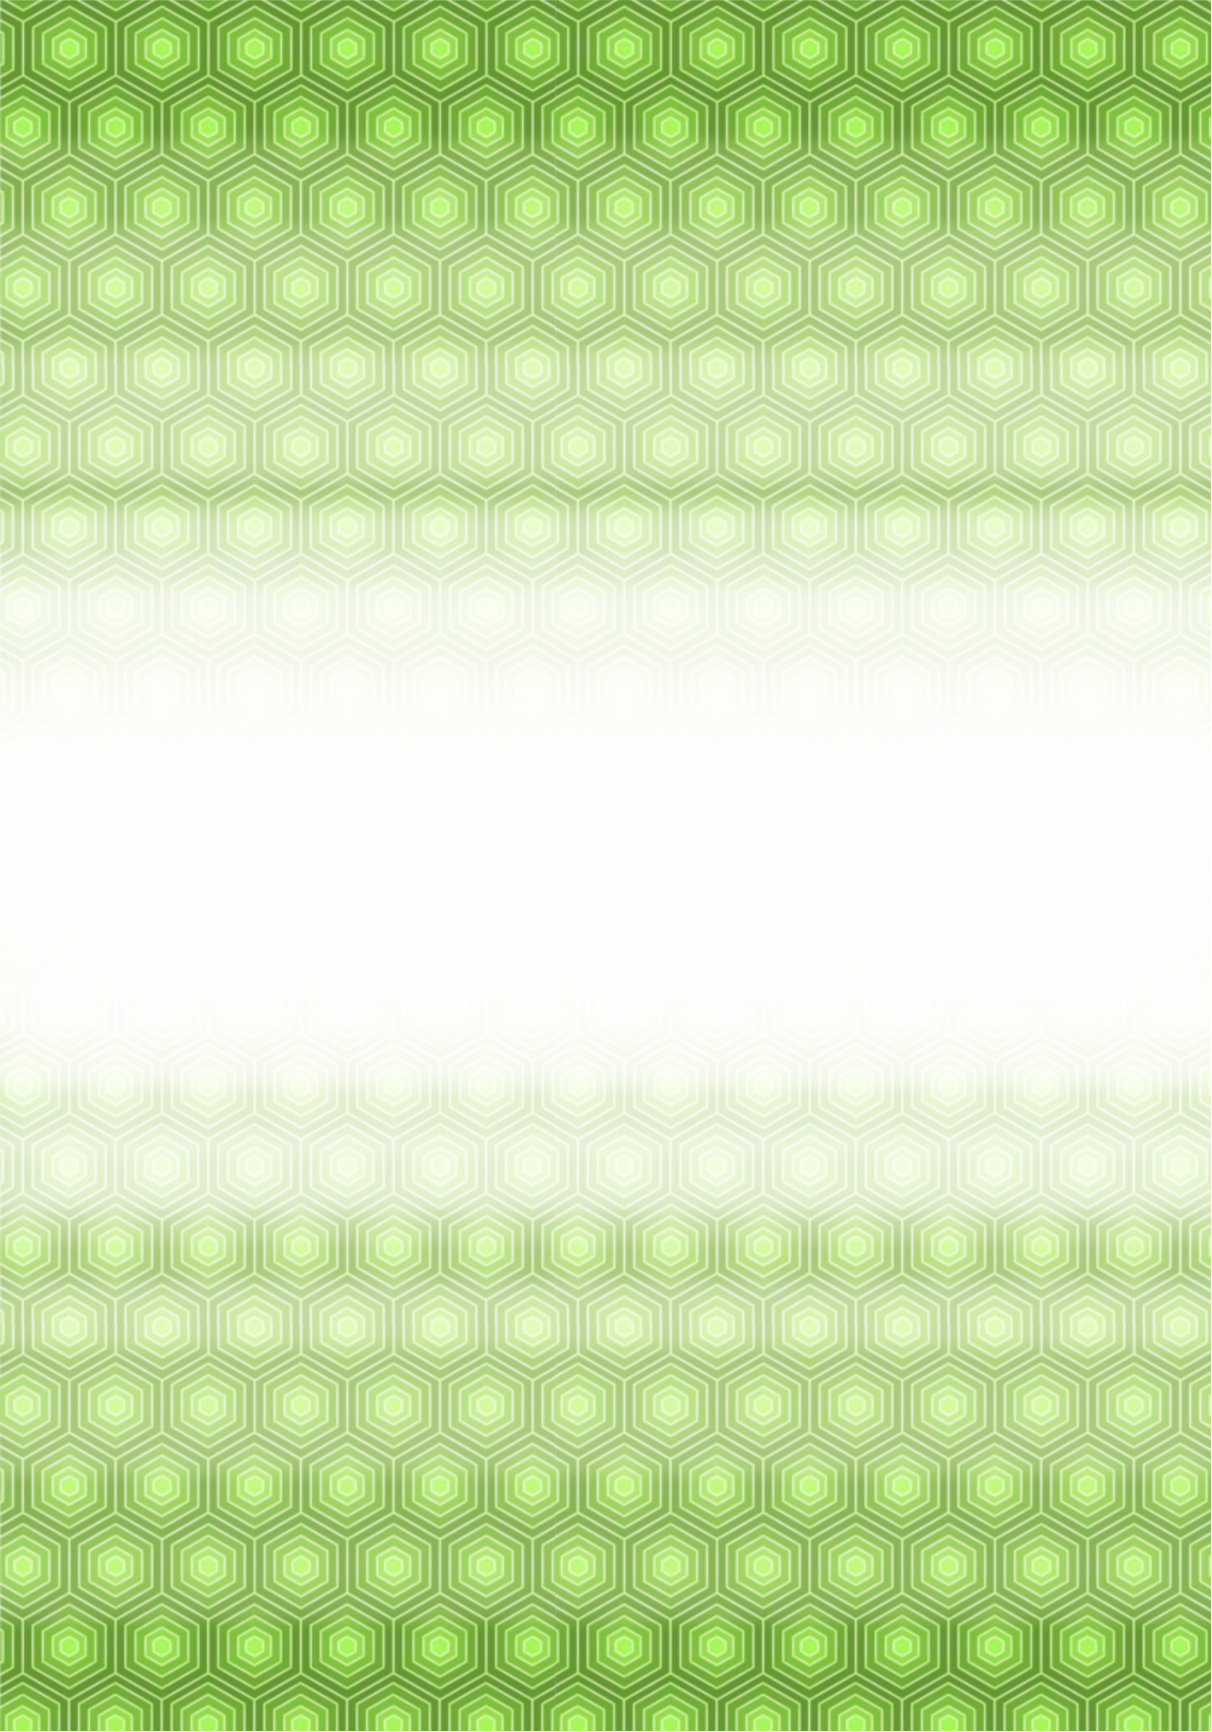
\includegraphics[scale=1]{cover}}} % Image background
\centering
\vspace*{3cm}
\begin{figure}[h]
\centering\hspace{30pt}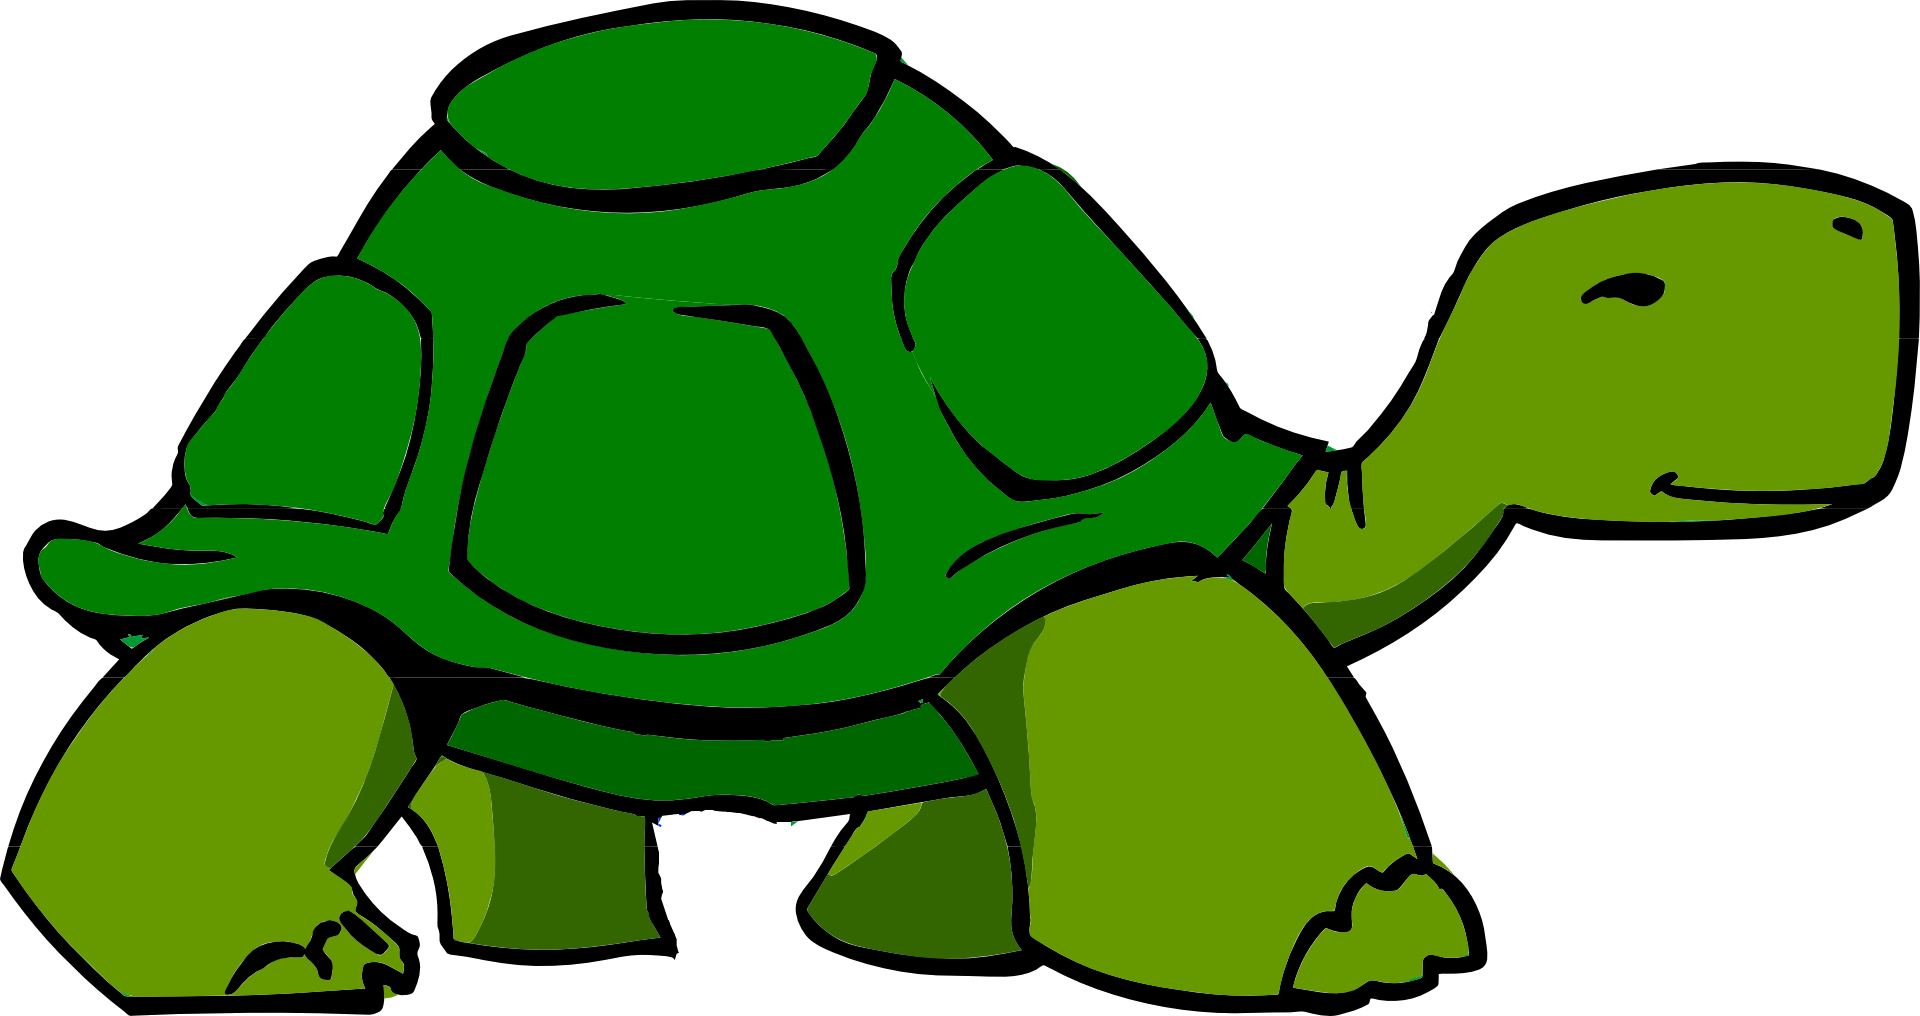
\includegraphics[scale=0.05]{turtle}
\end{figure}
\vspace*{1cm}
\par\normalfont\fontsize{50}{50}\sffamily\selectfont
ROS入門\\% Book title
{\Huge \textit{(Robot Operating System)}}\par
\vspace*{6cm}
{\large Yoonseok Pyo, Ryo Kurazume, Yuta Watanabe}\\
{\large Laboratory For Intelligent Robots \& Vision System\\Kyushu University in Japan}\par
\endgroup

%-------------------------------------------------------------------------------
% COPYRIGHT PAGE
%-------------------------------------------------------------------------------

\newpage
~\vfill
\thispagestyle{empty}

\noindent ROS入門\\

\noindent Copyright \copyright\ 2015\\by Yoonseok Pyo (\href{mailto:passionvirus@gmail.com}{passionvirus@gmail.com}), Ryo Kurazume, Yuta Watanabe\\ % Copyright notice

\noindent \textsc{Published by IRVS}\\ % Publisher

\noindent \textit{Ver 0.1.0, \today}\\ % Printing/edition date

% \noindent
% Special Thanks: 박형일, 이재상, 신경만, 김대근, 김성준, 유재성, 이용진, 이준규, 주용수, 진성주, 하광진, 한승록, Daniel, 이지훈, yukino040, 김영진, 한성 / 이 책이 나올 수 있었던 고마운 분들입니다. 다시 한번 감사 드립니다.


\begin{figure}[h]
\centering

\includegraphics[scale=0.3]{cc-logo}
\hspace{10pt}

\includegraphics[scale=0.5]{by-nc}
\end{figure}

\noindent この作品はクリエイティブ・コモンズ・表示 4.0 国際・ライセンスで提供されています。このライセンスのコピーを閲覧するには、 \url{http://creativecommons.org/licenses/by/4.0/} を訪問して下さい。\\

\noindent This work is licensed under the Creative Commons Attribution 4.0 International License. To view a copy of this license, visit \url{http://creativecommons.org/licenses/by-nc/4.0/}. Unless required by applicable law or agreed to in writing, software distributed under the License is distributed on an \textsc{``as is'' basis, without warranties or conditions of any kind}, either express or implied. See the License for the specific language governing permissions and limitations under the License.\\ % License information

% \noindent 이 저작물에서 사용된 (주)유진로봇의 Kobuki와 관련해서는 사용 허락을 받아 사용하였고, 본문에서 사용된 일부 이미지 및 템플릿에 대해서 별도의 라이선스를 가지고 있으며, 필자는 그 세부 사항을 아래에 표시합니다. 또한, 이 저작물에 사용된 이미지 중 본 저작물의 라이센스인 CC BY-NC 이외의 저작권을 갖는 이미지는 각 페이지에 별도로 표시합니다.\\

\noindent Background image of cover page and chapter head image\\
Free Turtle Pattern By freecooldesign (www.freecooldesign.com)\\
License: CC BY-NC 3.0\\

\noindent Turtle image of cover page\\
By Nemo (http://pixabay.com/en/turtle-green-shell-animal-reptile-304427/)\\
License : CC0 Public Domain\\

\noindent LaTeX template ``The Legrand Orange Book'' made by LaTeXTemplates.com\\
Original author (LaTeX template): Mathias Legrand (legrand.mathias@gmail.com)\\
License: CC BY-NC-SA 3.0\\

\noindent \textbf{We'd like to give special thanks to ROS development team, many ROS maintainers and contributors. We $\heartsuit$ ROS (\url{http://www.ros.org/})}

%-------------------------------------------------------------------------------
% TABLE OF CONTENTS
%-------------------------------------------------------------------------------

\chapterimage{chapter_head_14.pdf} % Table of contents heading image

\pagestyle{empty} % No headers

\tableofcontents % Print the table of contents itself

\cleardoublepage % Forces the first chapter to start on an odd page so it's on the right

\pagestyle{fancy} % Print headers again

%-------------------------------------------------------------------------------
% CHAPTER  LIST
%-------------------------------------------------------------------------------

\setlength\parindent{1em}
% !TEX root = ./rosbook_jp.tex
%-------------------------------------------------------------------------------
\chapterimage{chapter_head_1.pdf}

%-------------------------------------------------------------------------------
\chapter{ROS入門}

%-------------------------------------------------------------------------------
\section{ロボットソフトウェアプラットフォーム}\index{ロボットソフトウェアプラットフォーム}

1973年に発売された世界初の商用携帯電話Motorola DynaTAC  8000は、重量が0.8kgもあり、およそ携帯とは呼べないほど持ち運びに不便であった。しかし、現在のスマートフォンは、インターネット、SNS、メッセージ、ゲーム、音楽鑑賞など、さまざまな機能を備え、もはや日常生活に欠くことができない最も身近な機器となっている。
初期の携帯電話メーカーは、薄く軽量で、かつ長時間、高品質の通話を実現するために熾烈なハードウェア開発競争を繰り広げ、他社に先駆けて新しい機能を搭載した新製品を次々と投入した。また、新たな機器の性能を最大限に生かせるよう、特定の機種に対応したファームウェア(機器制御用基本ソフトウエア)を個別に開発していた。このため、新しいハードウェアが開発されるたびに、その開発スケジュールに合わせて新たにファームウェアを開発する必要があった。このようなハードウェアに重点を置いた開発は、ソフトウェア開発にかかる管理コストの増加をもたらし、開発スピードも徐々に低下していった。
この問題を解決するために、Android、iOS, Windows Phoneなど、特定のハードウェアに依存しないスマートフォン向けオペレーティングシステムが開発された。携帯電話メーカーはこれらを採用することで、管理コストを抑えつつ、新たな機能の追加が容易に行えるようになった。さらに、ハードウェアに精通していなくても関連アプリケーションが開発できるようになり、ハードウェアよりもソフトウェアにより重きを置いた「アプリ開発者」と呼ばれる新しい職種まで登場した。
以上のように、携帯電話およびスマートフォン市場の急成長は、2つの段階に分けられる。第1段階は、ハードウェアの発達と爆発的なユーザー数の増加に支えられていた。第2段階は、スマートフォン向けオペレーティングシステムの登場と、それによるアプリケーションの開発時間や管理コストの削減、開発者のすそ野の広がりに依るところが大きい。

%-------------------------------------------------------------------------------
\subsection{ロボットソフトウェアプラットフォームがもたらす変化}\index{ロボットソフトウェアプラットフォームがもたらす変化}

ロボット開発も、携帯電話やスマートフォンによく似た歴史を辿っている。従来、ロボット用アプリ開発者は、ロボットのハードウェア構成を強く意識した専用のソフトウェアを開発してきた。しかし、スマートフォンと同様に、汎用的なロボットオペレーティングシステム、あるいはソフトウェアプラットフォームが開発されれば、アプリ開発者はそこで動作するアプリケーション開発に資源を集中できる。ロボットソフトウェアプラットフォームは、スマートフォンの成長における初期の開発/発展段階にあり、少々乱立気味ともいえるほど多くの種類が発表されている。表1.1 に、特に広く利用され、開発が盛んなロボットソフトウェアプラットフォームと、その開発母体を示す。

ロボットソフトウェアプラットフォームの例

\begin{itemize}
\item ERSP\footnote{\url{http://www.evolution.com/products/ersp/}}、Evolution Robotics
\item MSRDS\footnote{\url{http://msdn.microsoft.com/en-us/robotics/default.aspx}}、Microsoft
\item MARIE\footnote{\url{http://marie.sourceforge.net/}}、LABORIUS
\item URBI\footnote{\url{http://www.urbiforge.org/}}、Gostai\footnote{\url{http://www.gostai.com/}}
\item ROS\footnote{\url{http://www.ros.org/}}、Open Source Robotics Foundation\footnote{\url{http://www.osrfoundation.org/}} 、(OSRF、米国)
\item OpenRTM\footnote{\url{http://www.openrtm.org}}、産業技術総合研究所 (AIST、 日本)
\item OROCOS\footnote{\url{http://www.orocos.org/}}、KU Leuven、LASS、KTHなどのヨーロッパ連合(ヨーロッパ)
\item OPRoS\footnote{\url{http://www.opros.or.kr/}}、ETRI、KIST、KITECH、江原大学(韓国)
\item NAOqi\footnote{\url{https://www.aldebaran.com/ja/naoqi-os}}、ソフトバンク(日本)、Aldebaran(フランス)
\end{itemize}

このように、これまでに様々なロボットソフトウェアプラットフォームが開発されているが、その優劣を一概に論じることは難しい。なぜなら、使いやすいコンポーネントの追加機能や通信機能、可視化、シミュレータ、リアルタイム性など、各プラットフォームがそれぞれユニークな機能を提供しているからである。しかし、現在のパーソナルコンピュータのオペレーティングシステム(OS)のように、ロボットソフトウェアプラットフォームも、いずれは淘汰され、統合されていくと予想される。
本書は、OSRF(Open Source Robotics Foundation)により開発、メンテナンスが行われているROS(Robot Operating System)の解説書である。ROSは、上述した多くのロボットソフトウェアプラットフォームの中でも、ユーザー数、提供ライブラリの種類と数、拡張性の高さ、開発の容易さなどの点で特に優れている。ROSコミュニティは世界各地で活発に活動しており、ROSコミュニティが中心となりWeb上に蓄積された数多くの資料から、利用中に生じた疑問点や不具合の情報を容易に得ることができる。さらに、ROSはOSRFが単独で開発しているのではなく、大学の研究者、企業の開発者、趣味で活動するハーベスト(hobbyist)、さらにはロボットを専門とする人々だけでなく、コンピュータサイエンス、コンピュータビジョン、あるいは通信ネットワークの専門家など、多様な人々が開発に携わっている点で特徴的である。

%-------------------------------------------------------------------------------
\subsection{ロボットソフトウェアプラットフォームがもたらす未来}\index{ロボットソフトウェアプラットフォームがもたらす未来}

ロボットソフトウェアプラットフォームを利用すると、ロボットのハードウェアに対する知識をそれほど持たなくても、ロボット用アプリケーションの開発が可能である。これは、最新のスマートフォンのハードウェア構成や詳細を知らなくとも、アプリを開発できることと同様である。
以前は、ロボット開発者、あるいはロボットメーカは、ハードウェアの設計からソフトウェア開発まで一貫して手掛けていた。しかし、ロボットソフトウェアプラットフォームに準拠すれば、ソフトウェアに精通した多様な人材がロボットアプリケーション開発に参加できる。一方、ハードウェア開発者は、ソフトウェアプラットフォームで提供するインターフェースに合わせてハードウェアを設計すればよい。これにより携帯電話と同様、ロボットメーカはアプリケーションの開発時間や管理コストを削減でき、ロボット分野が急速に発展するきっかけとなり得る。

%-------------------------------------------------------------------------------
\section{ROSとは}\index{ROSとは}

ロボットソフトウェアプラットフォーム一般について理解したところで、ここからはROSについて説明する。まずは、そもそもROSとは何なのかを明らかにしよう。
ROSの公式サイトであるROS Wiki注13では、ROSを以下のように定義している。

ROS (Robot Operating System)はソフトウェア開発者のロボット・アプリケーション作成を支援するライブラリとツールを提供しています。具体的には、 ハードウェア抽象化、デバイスドライバ、ライブラリ、視覚化ツール、 メッセージ通信、パッケージ管理などが提供されています。

つまり、ROSは異なるハードウェアでも共通して使用できるロボットオペレーティングシステムであり、アプリケーション開発のための様々なツールを備えたソフトウェアプラットフォームである。

%-------------------------------------------------------------------------------
\subsection{ROSは新しいオペレーティングシステム(OS)か}\index{ROSは新しいオペレーティングシステム(OS)か}

オペレーティングシステムには、汎用コンピュータ向けのものとしてWindows(Windows XP、7、8 ...)、Linux(Ubuntu、Fedora、Gentoo ...)、MAC(OS X Yosemite...)などがあり、スマートフォン向けのものとしてはAndroid、iOS、Symbian、RiMO、Tizenなどが有名である。Robot Operating Systemという名前から、特にROSに初めて接する読者は、ROSをこれらの汎用コンピュータ向けのオペレーティングシステムと同様なものと捉えているかもしない。しかし、より正確に表現すれば、ROSは図1-5に示すようなメタ・オペレーティングシステム(Meta-Operating System)である。メタ・オペレーティングシステムとは、オペレーティングシステム上で動作し、同一、あるいは異なるオペレーティングシステム(あるいはコンピュータ)で動作しているプロセスに対し、プロセス間通信やスケジューリング、負荷の監視、エラー処理などを支援するシステムである。つまり、ROSは、Windows、Linux、Androidに取って代わるロボットのためのオペレーティングシステムではなく、上記のオペレーティングシステムで動作するプロセスを制御するシステムである。
例えば、Linuxの頒布形態(ディストリビューション)であるUbuntu上で動作するROSは、Ubuntuのプロセス管理システム、ファイルシステム、ユーザインタフェース、プログラムユーティリティ(コンパイラ、スレッドモデルなど)などを利用している。ROSは、これに加えて様々なセンサやロボットなどのハードウェアの制御、プロセス間通信、スケジュール、エラー処理など、ロボットアプリケーションの開発に必要な機能をライブラリとして提供している。
またROSは、ROSを利用して開発された様々なアプリケーションパッケージを管理し、流通する仕組み(生態系、Ecosystem)を備えている。
このようにROSとは、既存の伝統的なオペレーティングシステムを利用しながら、ロボットアプリケーションの開発に必須となるロボットやセンサの制御システムを、ハードウェア抽象化の概念に基づいてパッケージ化したものである。さらに様々なアプリケーションもパッケージとして提供することで、ユーザーによるロボットアプリケーション開発を強力に支援する。

\begin{figure}[h]
  \centering
  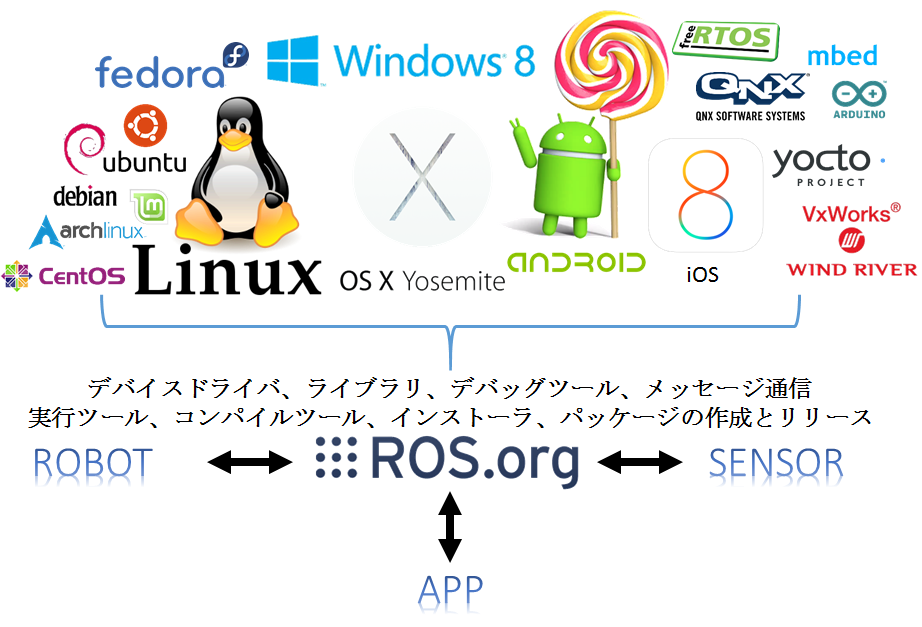
\includegraphics[width=\columnwidth]{pictures/chapter1/pic_01_01.png}
  \caption{メタ・オペレーティングシステムとしてのROS}
\end{figure}


また図1-1のように、ROSでプロセス間通信に使用されるメッセージは、異なるオペレーティングシステムや異なるハードウェア上のプロセス間でも自由に情報をやり取りすることができる。したがってROSは、様々なハードウェアから構成される複雑なロボットの開発にも適したオペレーティングシステムである。これについては、後半の章でより詳細に取り上げる。

\begin{figure}[h]
  \centering
  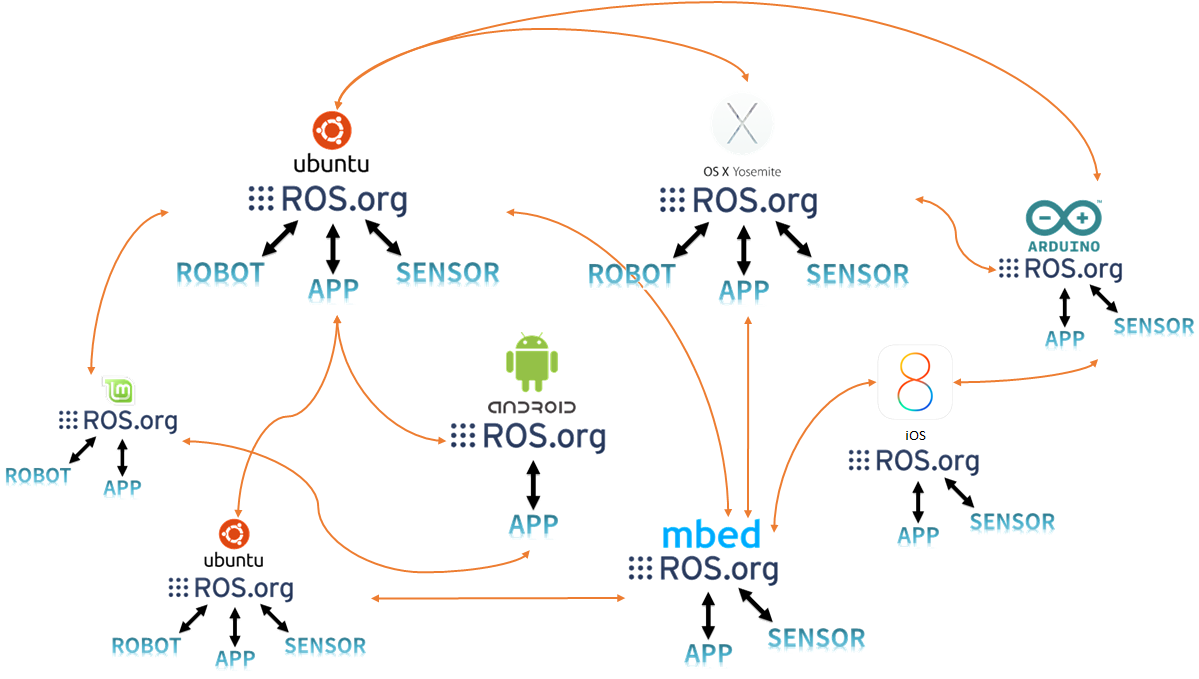
\includegraphics[width=\columnwidth]{pictures/chapter1/pic_01_02.png}
  \caption{異なるオペレーティングシステムやハードウェア上のプロセスに対する通信}
\end{figure}

%-------------------------------------------------------------------------------
\subsection{ROS生態系}\index{ROS生態系}

近年、Android、iOS、Symbian、RiMO、Tizenなどスマートフォン向けオペレーティングシステムの開発現場では、生態系(Ecosystem)、あるいはモバイル生態系という単語をよく耳にする。これは、スマートフォンの製造会社と販社、様々なアプリケーションを開発するサードパーティ、さらにユーザーが有機的に密に結びつけられたモデルのことである。例えば、スマートフォン製造会社がオペレーティングシステムで定められたインターフェースに合わせて機器を製造し、各オペレーティングシステム会社は、これに合わせたライブラリを作成して提供する。ソフトウェア開発者は提供されたライブラリを利用することで、ハードウェアの深い知識がなくても容易にサービスプログラムを開発できる。さらに、開発されたプログラムをユーザーが入手しやすいように流通させることで、収益が循環し、市場が成長する。この生態系には軸となるオペレーティングシステムが必要であり、パーソナルコンピュータ分野ではマイクロソフト社のWindows OSとフリーソフトウェアのLinuxがこれに当たる。
現在、ロボット分野でも同様の流れが見られる。つまり、当初は様々なハードウェアが乱立し、これらを統合するためのオペレーティングシステムが開発されていなかった。しかし現在では、様々なソフトウェアプラットフォームが提案され、特にROSはいち早く生態系の枠組みを整えつつある。今後、ロボット製造会社やセンサ製造会社などのロボット関連ハードウェアメーカー、およびROSの開発運用チームには、アプリ開発者やユーザーにも広く恩恵が及ぶようなROS生態系の確立が期待されている。

\begin{figure}[h]
  \centering
  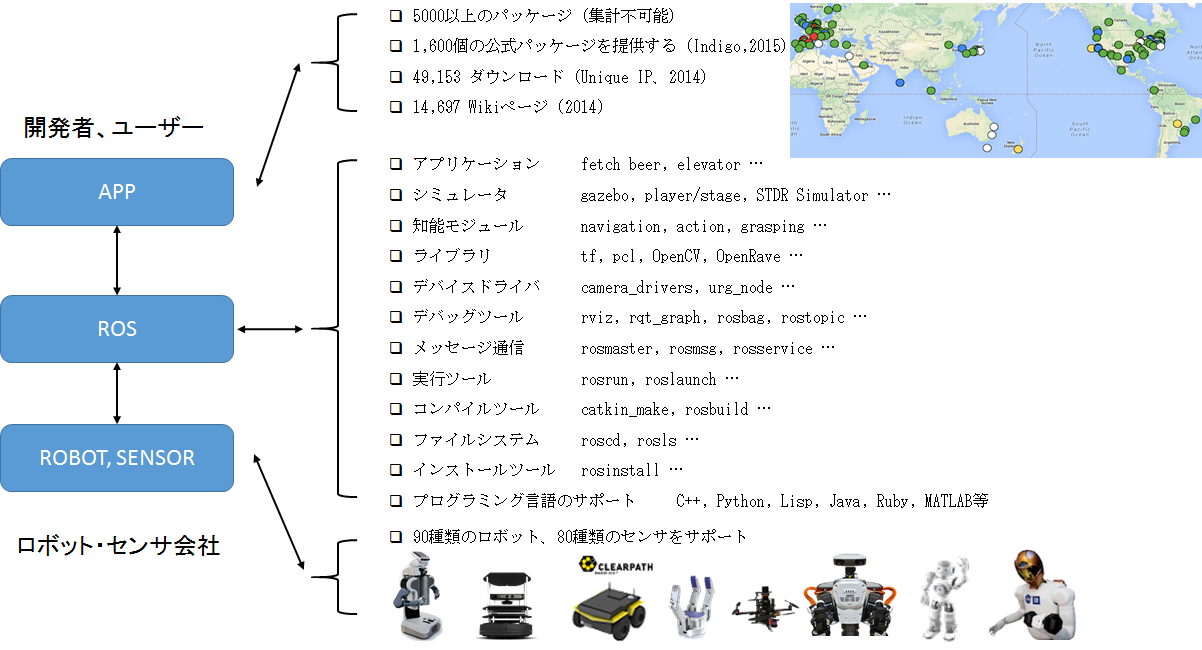
\includegraphics[width=\columnwidth]{pictures/chapter1/pic_01_03.png}
  \caption{ROS生態系}
\end{figure}

図1-7は、ROSCon2014注14で発表されたROS公式統計注15とROS Wikiデータ注16,17をもとにまとめたROSの現状である。まだ十分とはいえないが、ロボット分野でこれほど広く利用されているロボットソフトウェアプラットフォームは他にはなく、今後も成長が期待されている。

%-------------------------------------------------------------------------------
\section{ROSの歴史}\index{ROSの歴史}

ROSの技術的な詳細について述べる前に、ROSの歴史を振り返っておこう。 ROSは、2007年5月、米国のスタンフォード大学人工知能研究所(AI LAB)注18が実施したSTAIR(STanford AI Robot)プロジェクト注19において、Morgan Quigley注20が開発したSwitchyardに端を発する。2007年11月、米国のロボット専門企業Willow GarageがSwitchyardを引き継ぎ、ROSの名前で開発を始めた。Willow Garageは、パーソナルロボットとサービスロボットで著名な企業であり、有名な画像処理オープンソースソフトウエアであるOpenCV注23や、マイクロソフトKinectなどの3次元計測器で利用されるPCL(Point Cloud Library)注24をサポートしていたことでも知られる。

\begin{figure}[h]
  \centering
  
\includegraphics[width=\columnwidth]{pictures/chapter1/pic_01_04.png}
  \caption{ROSロゴ(http://wiki.ros.org/)}
\end{figure}

Willow Garageは、2010年1月22日にROSの開発者向けプレリリース版であるROS 1.0を発表した。その後、2010年3月1日にその公式バージョンであるROS Box Turtleがリリースされた。その後も、C Turtle、Diamondbackなど、UbuntuやAndroidと同様にABC順にバージョン名を付け、アップデートを続けている。 2014年7月にはROSの9番目のバージョンROSインディゴイグルー(Indigo Igloo、公式リリースでは、8番目のバージョン)を公開した。
ROSは、フリーソフトウェアの代表的なライセンス体系であるBSDライセンス(BSD 3-Clause License注25)をベースにしており、誰でも修正、再利用、再配布が可能である。開発者とユーザーを対象としたカンファレンス(ROSDay、ROSCon)が定期的に開催され、アメリカとヨーロッパではROS Industrial注26 (産業用途のROS)を開発しているコンソーシアムがある。また、それぞれの国で、ROS Meetupと呼ばれるコミュニティが、セミナーなどのイベントを開催している。日本でも、東京オープンソースロボティクス協会(TORK)注27やROS JAPAN Users Group注28が中心になってセミナーや勉強会を開催し、ROSの普及に努めている。一方、PR2(Personal Robot 2)注29やタートルボット(turtlebot)注30など、ROSの利用を前提としたロボット(リファレンスロボット)の開発も行われている。さらにこれらのリファレンスロボットを利用して多くのアプリケーション開発が行われ、これにより現在ではROSは最も標準的なロボットソフトウェアプラットフォームの一つとなっている。

%-------------------------------------------------------------------------------
\section{ROSのバージョン}\index{ROSのバージョン}

Willow GarageがSwitchyardをROS(Robot Operating System)という名前で引き継ぎ、その後7回のバージョンアップを経て、2012年12月にROS Groovy Galapagosバージョンをリリースした。
その後、2013年にWillow Garageが商業サービスロボット市場に参入し、ROSの開発はロボット向けのオープンソースソフトウエア財団であるOSRF(Open Source Robotics Foundation)注31に移譲された。OSRFは、2014年7月にROSの9番目のバージョンアップROS Indigo Iglooバージョンをリリースした。各リリースは図1-9に示すように亀をモチーフにしたシンボルで表されている。

ROSのリリース注32とコンファレンス注33
\begin{itemize}
\item  2015/05/30: Jade Turtleリリース
\item  2014/09/12: ROSCon2014カンファレンス開催
\item  2014/07/22: Indigo Iglooリリース
\item  2014/06/06: ROS Kong 2014開催
\item  2013/09/04: Hydro Medusaリリース
\item  2013/05/11: ROSCon2013カンファレンス開催
\item  2013/02/11: Open Source Robotics Foundationが開発、管理を務める
\item  2012/12/31: Groovy Galapagosリリース
\item  2012/05/19: ROSCon2012カンファレンス開催
\item  2012/04/23: Fuerteリリース
\item  2011/08/30: Electric Emysリリース
\item  2011/03/02: Diamondbackリリース
\item  2010/08/03: C Turtleリリース
\item  2010/03/01: Box Turtleリリース
\item  2010/01/22: ROS 1/0開発
\item  2007/11/01: Willow Garageが「ROS」という名前で開発を開始
\item  2007/05/01: Switchyard、Morgan Quigley、Stanford AI LAB、スタンフォード大学
\item  2000: Player/Stage Project、Brian Gerkey、Richard Vaughan、Andrew Howard、南カリフォルニア大学
\end{itemize}


\begin{figure}[h]
  \centering
  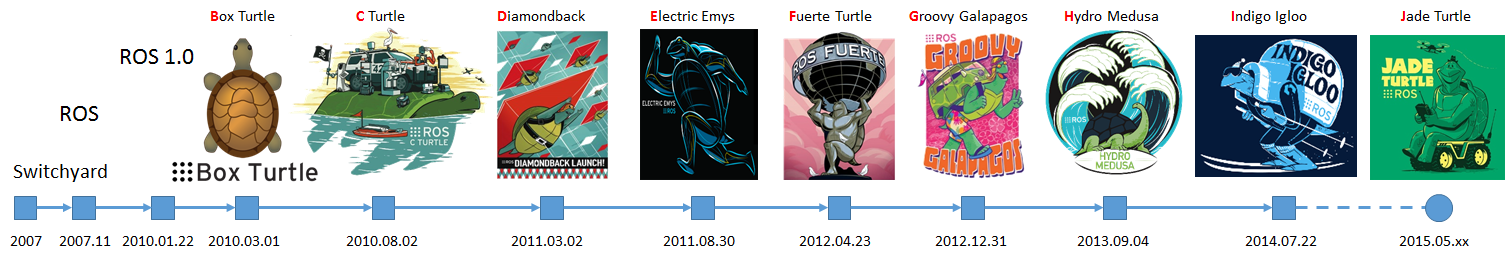
\includegraphics[width=\columnwidth]{pictures/chapter1/pic_01_05.png}
  \caption{ROSのバージョン(http://wiki.ros.org/)}
\end{figure}

%-------------------------------------------------------------------------------
\subsection{ROSのバージョンのルール}\index{ROSのバージョンのルール}

ROSはこれまでに、ROS 1.0、Box Turtle、C Turtle、Diamondback、Electric Emys、Fuerte、Groovy Galapagos、Hydro Medusa、Indigo Igloo、Jade Turtleの10のバージョンをリリースしている。ROSの各バージョンは、2つめのバージョン以降、その頭文字がアルファベット順になるように名づけられている(この命名方式は、UbuntuやAndroidと同様である)。つまり、現在多く使われているIndigo Iglooのバージョンは、アルファベットIバージョン、すなわち9番目のバージョンである。
また、図1-9と図1-10に示すように、各バージョンではポスター形式のイラストと亀のアイコンを発表している。この亀のアイコンは、turtlesim注34というROS公式チュートリアル用のシミュレーションにも使用されている。

\begin{figure}[h]
  \centering
  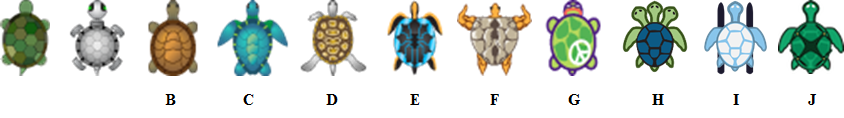
\includegraphics[width=\columnwidth]{pictures/chapter1/pic_01_06.png}
  \caption{各バージョンの亀のアイコン}
\end{figure}

%-------------------------------------------------------------------------------
\subsection{ROSリリースサイクル}\index{ROSリリースサイクル}

ROSが正式にサポートしているオペレーティングシステムはUbuntu注35であるため、Ubuntuの新バージョンのリリースサイクルと同様に、1年に2回(4月、10月)の更新が行われていた。しかし2013年、ROSの開発と管理を担当しているOSRFは、ユーザーの意見を取り入れて、Hydro Medusaバージョンから1年に1回、Ubuntuの新しいバージョンのリリースに合わせて4月か5月にリリースすることを発表した。
ROSのサポートは、一般的なUbuntuバージョンに合わせたものは1年間、2年に一度リリースされるUbuntu LTS(Long Term Support、例えばUbuntu 14.04)バージョンに合わせたものは、3年間サポートされる。例えば、2014年4月にリリースされたUbuntu 14.04 LTS(Trusty Tahr)に対応するROSのバージョンは、2014年のROS I版と2015年のJ版という2つのバージョンであり、それぞれ2017年4月までサポートされる予定である。現在までのUbuntu向けROSのリリースサイクル注36は、図1-11のとおりである。

\begin{figure}[h]
  \centering
  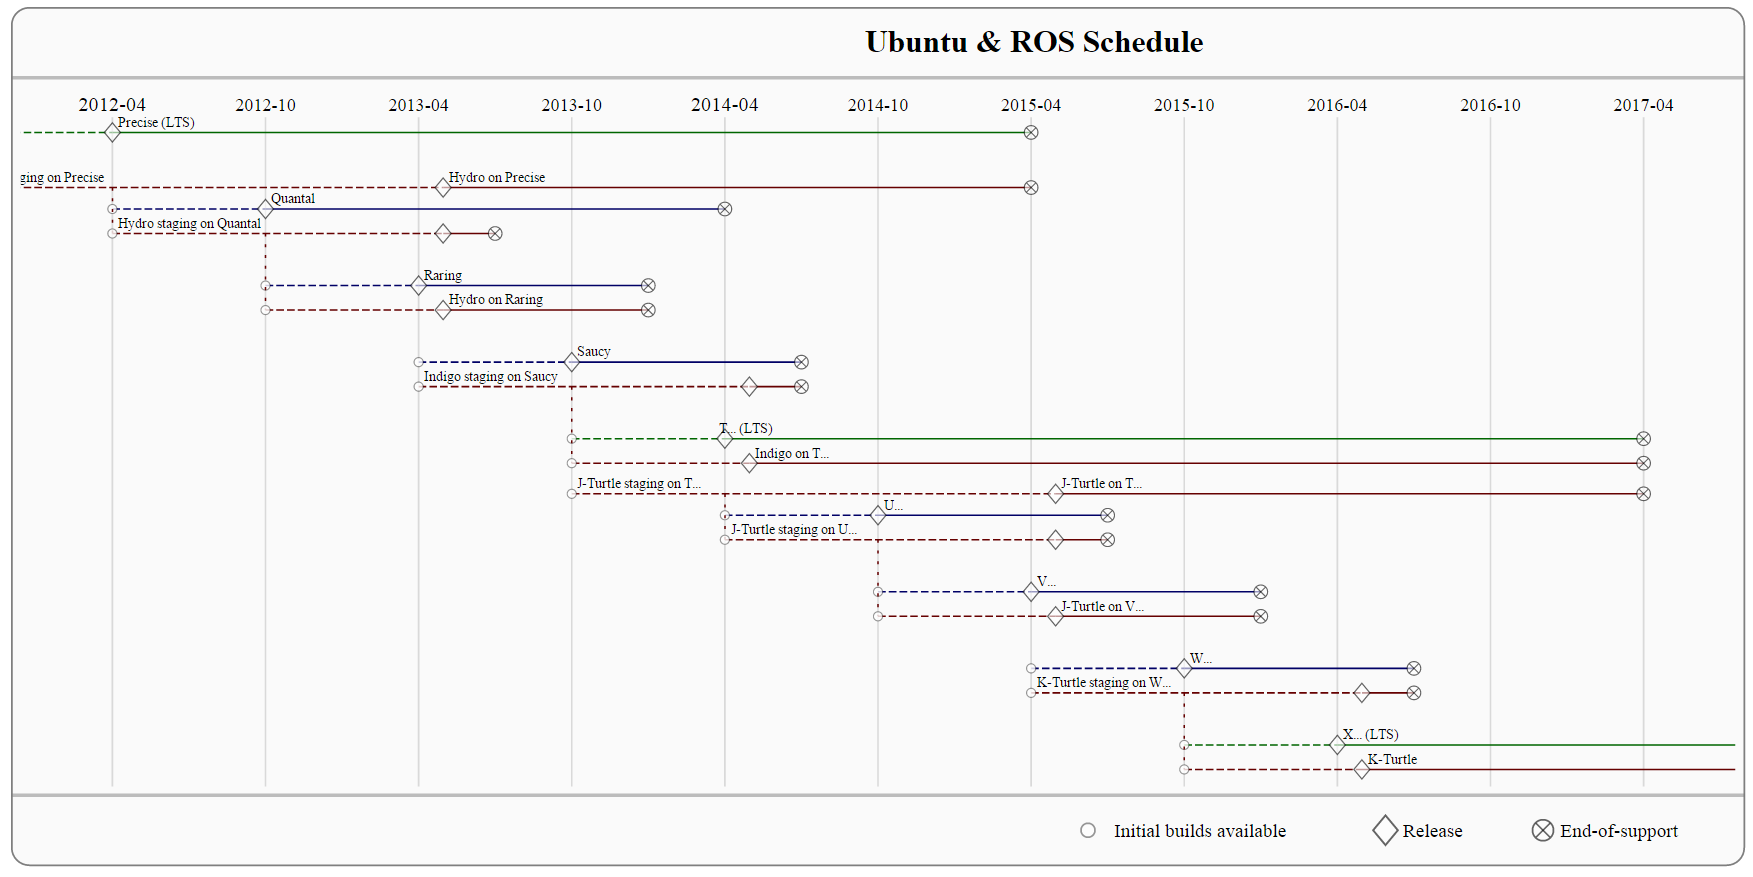
\includegraphics[width=\columnwidth]{pictures/chapter1/pic_01_07.png}
  \caption{Ubuntu向けROSのリリースサイクル}
\end{figure}


Ubuntuのリリースサイクルとサポート期間

Ubuntuは1年で2回、4月と10月にリリースされ、リリース時期によって14.04又は14.10などの名前が付けられている。また、2年間隔の偶数年度は、長期サポート版(Long Term Support)がリリースされる。これは、通常のバージョンが9ヶ月間サポートされるのに対し、LTSサポート期間はリリースから5年間である。LTSは安定した環境を望むユーザーに向いており、ROSユーザーもUbuntu LTSの公開に合わせてバージョンアップすることが多い。

http://ja.wikipedia.org/wiki/Ubuntu

%-------------------------------------------------------------------------------
\subsection{ROS Indigo Igloo}\index{ROS Indigo Igloo}

\begin{figure}[h]
  \centering
  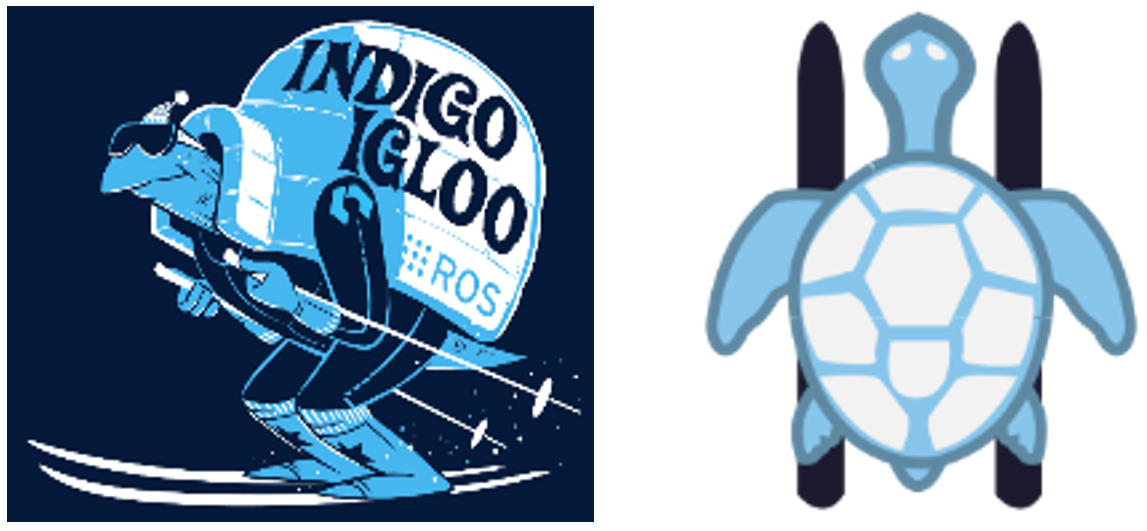
\includegraphics[width=\columnwidth]{pictures/chapter1/pic_01_08.png}
  \caption{Indigo Iglooのバージョンのポスターとアイコン}
\end{figure}

現在、ROSのコミュニティで最も使われているバージョンは、2014年7月22日に正式リリースされたROS Indigo Igloo注37である。ポスターは、亀がイグルー(ドーム状の家、Igloo)を背負ってスキーを楽しむ姿である。
このバージョンでは、特にcatkin注38ビルドシステムへの移行に重点を置き、すべてのパッケージがcatkin化された点が特徴的である。それに加え、今回のバージョンからPython3.3への対応や、OpenCVやPCLの標準ライブラリが使用されている。またcmake modulesという名前のパッケージがあり、これに公式サポートしていないパッケージを集約した。さらに、boostのsignal関数をすべてsignal2に変更し、最新のバージョンに対応した。全体的には、マイナーアップグレードとメンテナンスの色合いが強い。

%-------------------------------------------------------------------------------
\subsection{ROSバージョンの選択}\index{ROSバージョンの選択}

ROSはメタ・オペレーティングシステムであり、ROSを利用するには、まず基本的に使用するオペレーティングシステムを選択する必要がある。ROSはUbuntu、Mac OS X、Fedora、Gentoo、OpenSUSE、Debian、Arch Linux、Windowsなどの多くのオペレーティングシステムをサポートしているが、ROSのユーザーが最も多く使用しているオペレーティングシステムはUbuntuである。開発チームでもUbuntuのLTSバージョン注39に合わせて新バージョンをリリースしていることから、特に支障がない限り、UbuntuのLTSバージョンに合ったROSのバージョンを選択することが好ましい。
ROSの各バージョンにおけるUbuntuの対応状況に関する情報は、関連ROS Wikiサイトである「http://www.ros.org/debbuild/」にアクセスし、使用予定のROSのバージョンを選択することで得られる。このファイルには、現在選択しているROSのバージョンに対し、Ubuntuのバージョンごとに、既存のROSパッケージに対する最新のROSバージョンへの対応状況が記載されている。例えば、「http://www.ros.org/debbuild/indigo.html」では、図1-13のようにIndigo Iglooのバージョンの対応状況が確認できる。内容はパッケージの名前(Name)、パッケージのレポジトリ(Repo)、バージョン(Version)、開発やメンテナンスされているかの情報(Wet Status)、メインテナー(Maintainer)、各UbuntuとROSバージョンに対する移植状況等が記載されている。特に移植状況には注意する必要があるので、図1-13を例に説明する。

\begin{figure}[h]
  \centering
  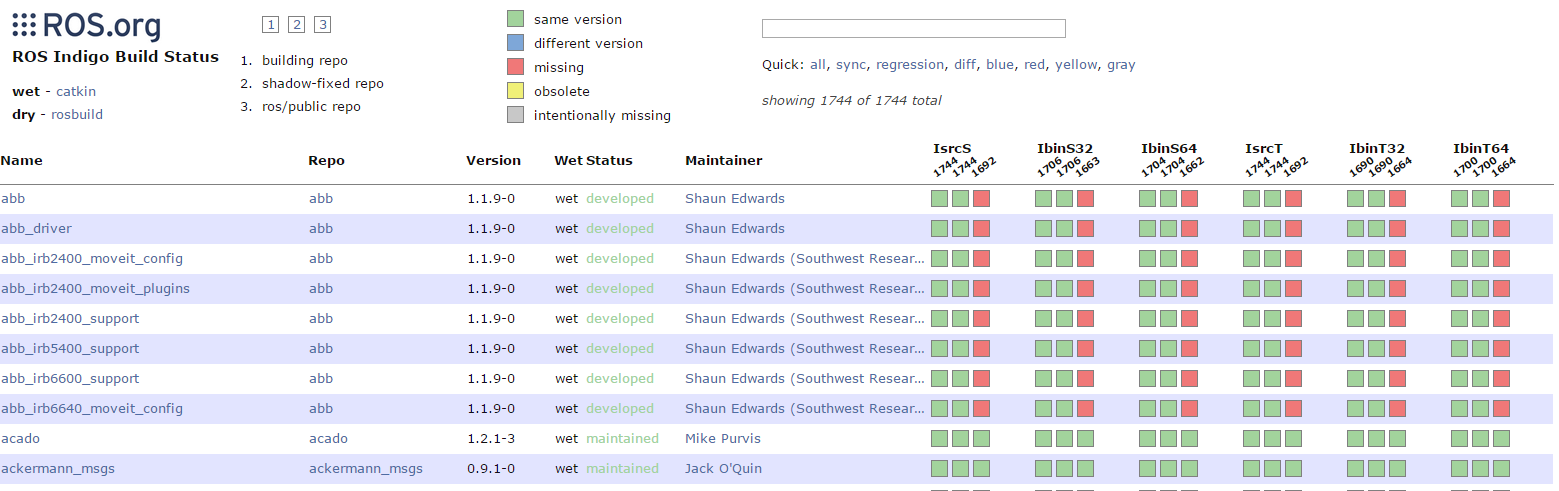
\includegraphics[width=\columnwidth]{pictures/chapter1/pic_01_09.png}
  \caption{Indigo Iglooのバージョンの移植状況}
\end{figure}

\begin{figure}[h]
  \centering
  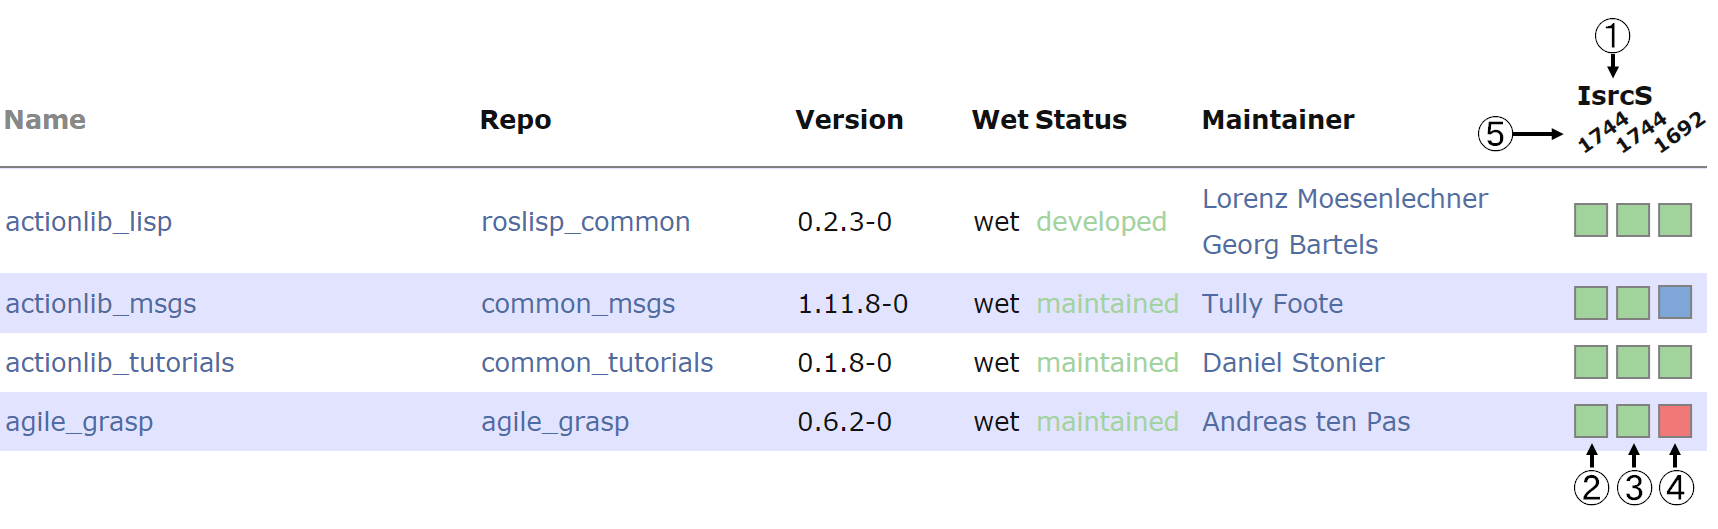
\includegraphics[width=\columnwidth]{pictures/chapter1/pic_01_10.png}
  \caption{Indigo Iglooのバージョンの移植状況の詳細}
\end{figure}

① IsrcS:ROS Indigo(I)バージョンのソース(src)のUbuntu 13.10 Saucy(S)バージョンに対する情報である。また、「IbinT64」の場合は、ROS Indigo(I)バージョンのバイナリ(bin)、64ビット Ubuntu 14.04 Trusty Tahr(T64)バージョンを意味する。
②、③、④ :色付きの四角のアイコンは、building, shadow-fixed, ros/publicを意味する。buildingは開発側のビルド状況、shadow-fixedは公式に出る直前のテストのためのレポジトリで、ros/publicは公式リリースされたレポジトリを示す。各色は、緑が問題なく移植された場合、青が以前のバージョンのままの場合、赤が移植できなかった場合、黄色が今回のバージョンに移植できないか、今後は使用しない場合、灰色は意図的に外したものである。
⑤ 番号:1744、1744、1692などは、それぞれbuilding, shadow-fixed, ros/publicで使えるパッケージの数を意味する。
ROSの最新バージョンへの移行を考える際、まず自分が使用したいパッケージがROSやUbuntuのバージョンに対応済みかを確認する必要がある。ROSの最新バージョンでは、多くのパッケージが「移植中」と表示されるが、使用したいパッケージ、および重要なパッケージが対応済みであれば最新バージョンに移行しても構わない。一方、もし使用したいパッケージが最新バージョンに対応していない場合には、移行は見合わせるべきである。

\begin{itemize}
\item Ubuntu 15.04: Vivid Vervet
\item Ubuntu 14.10: Utopic Unicorn
\item Ubuntu 14.04: Trusty Tahr(LTS)
\item Ubuntu 13.10: Saucy Salamander
\item Ubuntu 13.04: Raring Ringtail
\item Ubuntu 12.10: Quantal Quetzal
\item Ubuntu 12.04: Precise Pangolin(LTS)
\item Ubuntu 11.10: Oneiric Ocelot
\item Ubuntu 11.04: Natty Narwhal
\item Ubuntu 10.10: Maverick Meerkat
\item Ubuntu 10.04: Lucid Lynx(LTS)
\end{itemize}

本書では、2016年に次のUbuntu LTSバージョンがリリースされるまでは、以下の組み合わせを推奨する。

\begin{itemize}
\item オペレーティングシステム:Ubuntu 14.04 Trusty Tahr(LTS)
\item ROSのバージョン:ROS Indigo Igloo
\end{itemize}


% 注1 http://www.segye.com/content/html/2013/04/04/20130404004829.html
% 注2 http://www.evolution.com/products/ersp/
% 注3 http://msdn.microsoft.com/en-us/robotics/default.aspx
% 注4 http://marie.sourceforge.net/
% 注5 http://www.urbiforge.org/
% 注6 http://www.gostai.com/
% 注7 http://www.ros.org/
% 注8 http://www.osrfoundation.org/
% 注9 http://www.openrtm.org
% 注10 http://www.orocos.org/
% 注11 http://www.opros.or.kr/
% 注12 https://www.aldebaran.com/ja/naoqi-os
% 注13 http://wiki.ros.org/ROS/Introduction
% 注14 http://roscon.ros.org/
% 注15 http://wiki.ros.org/Metrics
% 注16 http://www.ros.org/browse/list.php
% 注17 http://www.ros.org/news/2012/12/ros-five-years.html
% 注18 http://ai.stanford.edu/
% 注19 http://stair.stanford.edu/
% 注20 http://www.osrfoundation.org/morgan-quigley.html
% 注21 http://playerstage.sourceforge.net/
% 注22 http://www.osrfoundation.org/brian-gerkey.html
% 注23 http://opencv.org/
% 注24 http://pointclouds.org/
% 注25 http://opensource.org/licenses/BSD-3-Clause
% 注26 http://rosindustrial.org/
% 注27 http://opensource-robotics.tokyo.jp/
% 注28 https://groups.google.com/forum/#!forum/ros-japan-users
% 注29 http://www.willowgarage.com/pages/pr2/overview
% 注30 http://turtlebot.com/
% 注31 http://osrfoundation.org/
% 注32 http://wiki.ros.org/Distributions
% 注33 http://roscon.ros.org/
% 注34 http://wiki.ros.org/turtlesim
% 注35 http://www.ubuntu.com/
% 注36 http://wiki.ros.org/Distributions/Timeline
% 注37 http://wiki.ros.org/indigo/
% 注38 http://wiki.ros.org/catkin
% 注39 https://wiki.ubuntu.com/Releases

%-------------------------------------------------------------------------------

% !TEX root = ./rosbook_jp.tex
%-------------------------------------------------------------------------------
\chapterimage{chapter_head_2.pdf}

%-------------------------------------------------------------------------------
\chapter{ROS のインストール}

1章で述べたように、ROSは多くのオペレーティングシステムで動作する。しかし、Ubuntu以外のOSは実験的な提供(Experimental)とされており、公式にはサポートされていない。そこで本書では、操作性や導入のしやすさから、UbuntuにインストールされたROSの使用を前提とする。本書で利用するROSの開発環境は、次の通りである。

\begin{itemize}
\item ハードウェア:IntelやAMD製CPUを内蔵したデスクトップおよびノートパソコン
\item オペレーティングシステム:Ubuntu 14.04 LTS または14.04.2 LTS(Trusty Tahr)
\item ROS: Indigo Igloo
\end{itemize}

もしコンピュータにインストールされているUbuntuのバージョンが異なる場合は、対応状況を公式サイト\footnote{\url{http://wiki.ros.org/indigo/Installation/Ubuntu}}で確認する必要がある。オペレーティングシステムがOS XまたはWindowsであれば、それぞれのインストール方法を関連Wiki\footnote{\url{http://wiki.ros.org/indigo/Installation/OSX/Homebrew/Source},\url{http://wiki.ros.org/hydro/Installation/Windows}} で確認されたい。

\begin{figure}[h]
  \centering
  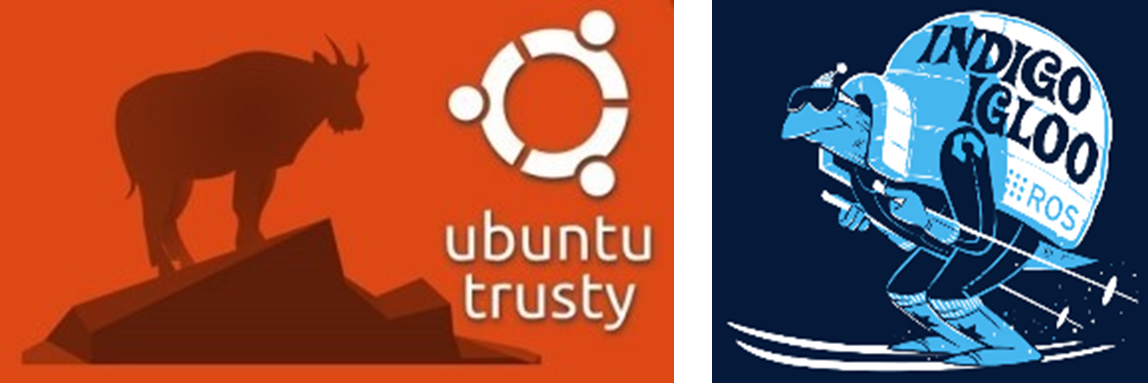
\includegraphics[width=0.9\columnwidth]{pictures/chapter2/pic_02_01.png}
  \caption{UbuntuのTrustyバージョンとROS Indigoバージョンのロゴ}
\end{figure}

%-------------------------------------------------------------------------------
\section{ROS Indigo のインストール}\index{ROS Indigo のインストール}

%-------------------------------------------------------------------------------
\subsection{ROS Indigo の一般的なインストール方法}\index{ROS Indigo の一般的なインストール方法}

まずROS Indigoのインストール方法について説明する。ただし、以下のインストール手順の説明に登場するソースリストやキーのアドレスは,OSRF財団の運営方針が変わると変更される場合もある。その時は注1のWikiサイトを参照してほしい。

\begin{exercise}[Ubuntuの14.04.2 LTS使用時の問題点]
  2015年2月17日に更新された14.04.2 LTSにROSパッケージをインストールする際、ibgl1-mesa-dri関連の依存関係の問題が起こる。そのため、Ubuntu 14.04.2 LTSをインストールした場合には、ROSをインストールする前に、以下のコマンドを実行して、依存関係ファイルをインストールする必要がある。
  \begin{lstlisting}[language=ROS]
  $ sudo apt-get install libgl1-mesa-dev-lts-utopic
  \end{lstlisting}
\end{exercise}

\subsubsection{NTP(Network Time Protocol) 設定}
ROSの公式な設定項目には含まれてないが、本書では複数のPCでROSを利用することを想定し、NTPの設定を行う。NTPはネットワーク上のPCで時刻同期を行うものである\footnote{\url{http://wiki.ros.org/ROS/NetworkSetup}} 。ROSの基準時間であるROS Timeが各PC間で異なっていると、通信処理に問題が生じるため、以下の2つのコマンドで各PC間のROS Timeを揃える。まず、最初の行のapt-getコマンドでchronyをインストールした後、次の行のntpdateコマンドでntpサーバをntp.ubuntu.com等に指定する。

\begin{lstlisting}[language=ROS]
$ sudo apt-get install chrony
$ sudo ntpdate -q ntp.ubuntu.com
\end{lstlisting}

これにより、各PCの時刻が指定したntpサーバの時刻に同期する。

\subsubsection{ROSリポジトリアドレスの追加}

次のように、ros-latest.listにROSリポジトリアドレスを追加する。

\begin{lstlisting}[language=ROS]
$ sudo sh -c 'echo "deb http://packages.ros.org/ros/ubuntu $(lsb_release -sc) main" > /etc/apt/sources.list.d/ros-latest.list'
\end{lstlisting}

\subsubsection{キーの設定}

ROSリポジトリからパッケージをダウンロードするために公開鍵を追加する。次のように入力する。

\\
\begin{lstlisting}[language=ROS]
$ wget https://raw.githubusercontent.com/ros/rosdistro/master/ros.key -O - | sudo apt-key add -
\end{lstlisting}

\subsubsection{パッケージインデックスの更新}

ソースリストにROSリポジトリアドレスを追加したので、以下のコマンドでパッケージリストをアップデートする。必須ではないが、ROSのインストール前に、インストール済みのUbuntu関連の全てのパッケージを最新のものにしておくとよい。

\\
\begin{lstlisting}[language=ROS]
$ sudo apt-get update && sudo apt-get upgrade
\end{lstlisting}

\subsubsection{ROS Indigo Iglooのインストール}

次のコマンドで、デスクトップ用の基本的なROSパッケージをインストールする。ここには、ROS、rqt、RViz、モデルや位置推定などのロボット関連のライブラリ、シミュレーション、ナビゲーションなどが含まれる。rqtとは、標準的なグラフィカルユーザインタフェースであるQTを利用したROS GUI開発ツールであり、RVizはROS標準の3次元可視化ツールである。これらは5章でより詳細に取り上げる。

\begin{lstlisting}[language=ROS]
$ sudo apt-get install ros-indigo-desktop-full
\end{lstlisting}

上記のコマンドを実行すれば基本的なrqtはインストールされるが、本書ではrqt関連のすべてのパッケージをインストールすることを推奨する。次のコマンドでrqt関連のすべてのパッケージがインストールでき、これにより様々なrqtプラグインが利用できる。

\begin{lstlisting}[language=ROS]
$ sudo apt-get install ros-indigo-rqt*
\end{lstlisting}

\begin{exercise}[ROSパッケージのバイナリのインストール]
  他のROSパッケージをインストールしたい場合には、次のようにapt-cacheのコマンドを利用して、ros-indigoで始まるパッケージを検索する。現在、以下のコマンドを実行すると、約1,600個のパッケージを確認することができる。

  \begin{lstlisting}[language=ROS]
  $ sudo apt-cache search ros-indigo*
  \end{lstlisting}

  個々のパッケージをインストールしたい場合は、次のコマンドでインストールする。

  \begin{lstlisting}[language=ROS]
  $ sudo apt-get install ros-indigo-%*[パッケージ名]*)
  \end{lstlisting}

  apt-cacheやapt-getコマンド以外にも、GUIツールであるsynaptic package managerを利用することもできる。
\end{exercise}

\begin{exercise}[APT(Advanced Packaging Tool)]
  apt-get、apt-key、apt-cache等で出てくるaptはAdvanced Packaging Toolの略語で、Ubuntuを含めDebian系列のLinuxでよく使用されるパッケージ管理コマンドである。

  http://en.wikipedia.org/wiki/Advanced\_Packaging\_Tool
\end{exercise}

\begin{exercise}[以前のバージョンのROSの削除と他のROSバージョンの併用]
  sudo apt-get purge ros-[以前のバージョン]-*コマンドで、以前のバージョンに関連したすべてのファイルが削除できる。もし、既存のバージョンと併用したい場合には、.bashrcに追加したROS設定ファイルを取得するコマンドの中で

  \begin{lstlisting}[language=ROS]
source /opt/ros/indigo/setup.bash
  \end{lstlisting}

  太文字を利用したいバージョンに変更すれば、複数のバージョンのROSを切り替えて利用できる。

 ※Ubuntuのバージョンが利用したいROSバージョンをサポートしている時のみ可能。1章参照のこと。
\end{exercise}

\subsubsection{rosdepの初期化}
ROSをインストールした後は、一度rosdepを初期化する必要がある。rosdepとは、rosの主要コンポーネントの使用時、もしくはコンパイル時に、依存関係にあるパッケージのインストールを容易にするツールである。

\begin{lstlisting}[language=ROS]
$ sudo rosdep init
$ rosdep update
\end{lstlisting}

\subsubsection{rosinstallのインストール}
続いて、ROSの様々なパッケージを容易にインストールするためのプログラムであるrosinstallをインストールしよう。必須ではないが、使用頻度が高く便利なツールであることから、本書ではrosintallのインストールを推奨する。

\begin{lstlisting}[language=ROS]
$ sudo apt-get install python-rosinstall
\end{lstlisting}

\subsubsection{環境設定ファイルのロード}

環境設定ファイルをロードする。 ファイルにはROS\_ROOT、ROS\_PACKAGE\_PATHなどの環境変数が定義されている。

\begin{lstlisting}[language=ROS]
$ source /opt/ros/indigo/setup.bash
\end{lstlisting}

\subsubsection{作業フォルダの作成と初期化}

ROSはcatkinというROS専用ビルドシステムを使用している。これを使用するには、次のコマンドでcatkin作業フォルダを作成し、作業フォルダ内の初期化を行う必要がある。この設定はROSインストールの後に一度だけ行えばよい。

\begin{lstlisting}[language=ROS]
$ mkdir -p ~/catkin_ws/src
$ cd ~/catkin_ws/src
$ catkin_init_workspace
\end{lstlisting}

catkin作業フォルダを作成した後、試しに作業フォルダ内のプログラムをビルドしてみよう。この時点では、catkin作業フォルダにはsrcフォルダとその中のCMakeLists.txtというファイルしか入っていないが、次のようにcatkin\_makeコマンドを使用してビルドする。

\begin{lstlisting}[language=ROS]
$ cd ~/catkin_ws/
$ catkin_make
\end{lstlisting}

問題なくビルドが完了したら、次のようにlsコマンドでフォルダの中身を確認しよう。

\begin{lstlisting}[language=ROS]
$ ls
build devel src
\end{lstlisting}

既にあるsrcフォルダのほかに、buildフォルダ、develフォルダが新たに作成されているのが分かる。catkinビルドシステムのビルドに関連するファイルはbuildフォルダに、実行に関連するファイルはdevelフォルダに保存される。
最後に、catkinビルドシステムに関連する環境ファイルを呼び出そう。

\begin{lstlisting}[language=ROS]
$ source ~/catkin_ws/devel/setup.bash
\end{lstlisting}

\subsubsection{テスト}
これで、ROSのインストールがすべて終了した。正しくインストールされたかを確認するため、一度すべてのターミナルウィンドウを閉じて、新しいターミナルウィンドウを開き、次のコマンドを入力してroscoreを実行してみよう。

\begin{lstlisting}[language=ROS]
$ roscore
\end{lstlisting}

次のようにエラーがなく実行された場合、インストールは正しく完了している。

\begin{lstlisting}[language=ROS]
$ roscore
... logging to /home/rt/.ros/log/f4b17da6-ecda-11e4-a7bf-d43d7e970cb0/roslaunch-rt-18869.log
Checking log directory for disk usage. This may take a while.
Press Ctrl-C to interrupt
Done checking log file disk usage. Usage is <1GB.

started roslaunch server http://192.168.4.100:47915/
ros_comm version 1.11.10


SUMMARY
========

PARAMETERS
 * /rosdistro: indigo
 * /rosversion: 1.11.10

NODES

auto-starting new master
process[master]: started with pid [18881]
ROS_MASTER_URI=http://192.168.4.100:11311/

setting /run_id to f4b17da6-ecda-11e4-a7bf-d43d7e970cb0
process[rosout-1]: started with pid [18894]
started core service [/rosout]
\end{lstlisting}

ROSを終了するには、<Ctrl>+<c>を押す。

%-------------------------------------------------------------------------------
\subsection{ROS Indigo の簡単インストール}\index{ROS Indigo の簡単インストール}

2.1.1項ではROS標準のインストール方法について説明したが、Ubuntuのバージョンが13.10か14.04であれば、前述したROSのインストールを自動的に実行するスクリプトを準備した。これを利用すれば、容易にROSをインストールできる。
※ただし、インストールできるROSのバージョンはIndigoのみである。

\begin{lstlisting}[language=ROS]
$ wget https://raw.githubusercontent.com/irvs/rosbook/master/ros_indigo_install.sh
$ sh ros_indigo_install.sh
\end{lstlisting}

%-------------------------------------------------------------------------------
\section{ROS の開発環境の構築}\index{ROS の開発環境の構築}

%-------------------------------------------------------------------------------
\subsection{ROS の環境設定}\index{ROS の環境設定}

ここまででROSがインストールできたので、次にROSが実行できるようにUbuntuの環境設定を行う。以下に示す手順で環境設定を行わない場合、ROSのインストールの途中で行った環境設定ファイルの読み込みは、新しいターミナルウィンドウを開く度に、次のコマンドにより行わなければならない。

\begin{lstlisting}[language=ROS]
$ source /opt/ros/indigo/setup.bash
$ source ~/catkin_ws/devel/setup.bash
\end{lstlisting}

これは非常に煩わしいので、新しいターミナルウィンドウを開くたびに、定められた環境設定ファイルを読み込むように設定する。またそれに加えて、ROSネットワークの設定や、頻繁に使用するコマンドの短縮形を登録しておくとよい。以下で手順を説明する。
まず、geditなどの文書編集プログラムを使用して、ユーザーのホームディレクトリ(/home/[ユーザー名]/)にある「.bashrc」ファイルを変更しよう。次のコマンドで「.bashrc」ファイルを開く。文章編集プログラムとして、gedit以外にsublime text、vim、emacs、nanoなどを使用しても構わない。

\begin{lstlisting}[language=ROS]
$ gedit ~/.bashrc
\end{lstlisting}

「.bashrc」ファイルを読み込むと、既に多くの環境設定がされている。設定済みの部分には触れずに、「.bashrc」ファイルの一番下までスクロールし、次の内容を追加する。6行目のxxx.xxx.xxx.xxxには、使用しているPCのIPアドレスを入れる。IPアドレスは「ifconfig」コマンドで確認できる。

~/.bashrc ファイルの追加部分
\begin{lstlisting}[language=bash]
1: # Set ROS Indigo
2: source /opt/ros/indigo/setup.bash
3: source ~/catkin_ws/devel/setup.bash
4:
5: # Set ROS Network
6: export ROS_HOSTNAME=xxx.xxx.xxx.xxx
7: export ROS_MASTER_URI=http://${ROS_HOSTNAME}:11311
8:
9: # Set ROS alias command
10: alias cw='cd ~/catkin_ws'
11: alias cs='cd ~/catkin_ws/src'
12: alias cm='cd ~/catkin_ws && catkin_make'
\end{lstlisting}

「.bashrc」ファイルを保存した後、修正された「.bashrc」ファイルの設定を反映させるために、現在開いているターミナルウィンドウで次のコマンドを入力する。

\begin{lstlisting}[language=bash]
$ source ~/.bashrc
\end{lstlisting}

%-------------------------------------------------------------------------------
\subsubsection{ROSの環境設定ファイルの読み込み}

「.bashrc」ファイルで、「#」で始まる行はコメント行であり、設定に影響を与えない。追加部分の2行目の「source /opt/ros/indigo/setup.bash」と3行目の「source ~/catkin\_ws/devel/setup.bash」を設定することで、ターミナル起動時にROSの環境設定ファイルが読み込まれる。

%-------------------------------------------------------------------------------
\subsubsection{ROSネットワーク設定}

「.bashrc」の追加部分の6~7行目はROSネットワークに関する記述であり、ROS\_MAS TER\_URIとROS\_HOSTNAMEを設定する意味をもつ。ROSはTCP/IPネットワークを利用した通信を行うため、この設定は極めて重要である。現段階では、どちらも使用しているPCのIPアドレスを入力すれば良い。今後、ROSネットワーク全体を統括するPC(マスターPC、roscoreを起動するPC)が一台だけ別にあり、複数台のロボットでそれぞれマスターPCとは異なるPC(ホストPC)を使用する場合、これらを分けて入力すると、異なるPC間で通信が可能になる。次に、マスターPC、ホストPCともに現在使用しているPCであり、このPCのIPアドレスが192.168.4.100である場合の設定例を示す。

\begin{lstlisting}[language=bash]
# Set ROS Network
export ROS_HOSTNAME=192.168.4.100
export ROS_MASTER_URI=http://${ROS_HOSTNAME}:11311
\end{lstlisting}

\begin{exercise}[ifconfig]
  Linuxで使用しているPCのIPアドレスを調べるには、ifconfigコマンドを利用する。以下の例のようにターミナルウィンドウでifconfigを実行してみよう。有線ならeth、無線であればwlanの項目で、inet addr以降の部分が使用しているPCのIPアドレスである。次の例では、有線接続時のIPアドレスは192.168.4.100である。
  \begin{lstlisting}[language=ROS, backgroundcolor=\color{ocre!10}, numbers=none]
  $ ifconfig
  eth0 Link encap:Ethernet HWaddr xx:xx:xx:xx:xx:xx
  inet addr:192.168.4.100 Bcast:192.168.4.255 Mask:255.255.255.0
  inet6 addr: fexx::d6xx:7exx:f1xx:xx2/64 Scope:Link

  lo  Link encap:Local Loopback
  inet addr:127.0.0.1 Mask:255.0.0.0 inet6 addr: ::1/128 Scope:Host

  wlan1 Link encap:Ethernet HWaddr xx:xx:xx:xx:xx:xx
  inet addr:192.168.4.200 Bcast:192.168.4.255 Mask:255.255.255.0
  inet6 addr: fexx::23xx:dfxx:fexx:5exx/64 Scope:Link
  \end{lstlisting}
\end{exercise}

%-------------------------------------------------------------------------------
\subsubsection{短縮コマンドの設定}

前掲の「.bashrc」の追加部分の10~12行目からは、ROSの開発作業で頻繁に使用するコマンドの短縮形を設定している。

\begin{itemize}[leftmargin=*]
\item cw:あらかじめ設定しておいたcatkin作業フォルダである~/catkin\_wsに移動
\item cs:catkin作業フォルダの中のソースファイルのフォルダである~/catkin\_ws/srcに移動
\item cm:catkin作業フォルダの~/catkin\_wsに移動した後、catkin\_makeコマンドでROSパッケージをビルド
\end{itemize}

\begin{exercise}[ROSの環境設定を確認する方法]
  次のように「export|grep ROS」コマンドを利用してROSの環境設定を確認できる。

  \begin{lstlisting}[language=bash]
  $ export | grep ROS
  declare .x ROS_DISTRO="indigo"
  declare .x ROS_ETC_DIR="/opt/ros/indigo/etc/ros"
  declare .x ROS_HOSTNAME="192.168.4.100"
  declare .x ROS_MASTER_URI="http://192.168.4.100:11311"
  declare .x ROS_PACKAGE_PATH="/home/xxx/catkin_ws/src:/opt/ros/indigo/share:/opt/ros/indigo/ stacks"
  declare .x ROS_ROOT="/opt/ros/indigo/share/ros"
  declare .x ROS_TEST_RESULTS_DIR="/home/xxx/catkin_ws/build/test_results"
  \end{lstlisting}
\end{exercise}


%-------------------------------------------------------------------------------
\subsection{ROSの動作テスト}\index{ROSの動作テスト}

ROSをインストールした後、正常に動作するかを確認するために、ROSが提供する簡単なノード(☞用語集P.XXX)の実行方法について説明する。使用するのはturtlesimというパッケージで、これは、ROSのシンボルである亀が画面に表示され、キーボード操作によって移動するプログラムである。

%-------------------------------------------------------------------------------
\subsubsection{roscoreの実行}

新しいターミナルウィンドウを開いて、次のコマンドを実行する。これにより、すべてのROSシステムを管理するroscoreが起動される。

\begin{lstlisting}[language=ROS]
$ roscore
\end{lstlisting}

\begin{figure}[h]
  \centering
  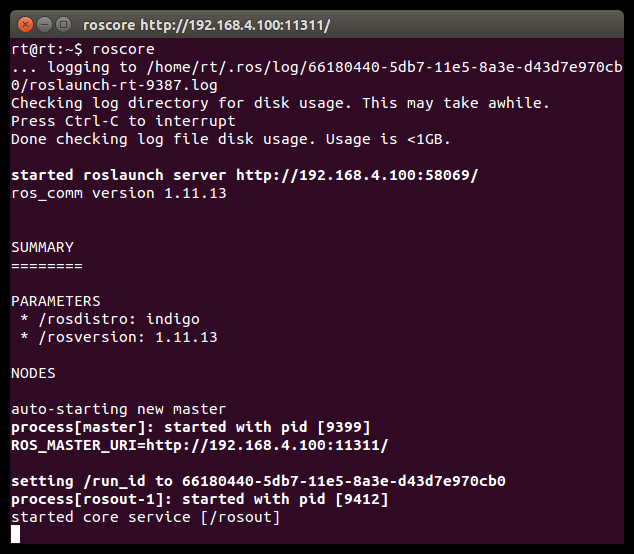
\includegraphics[width=0.9\columnwidth]{pictures/chapter2/pic_02_02.png}
  \caption{roscoreが起動された画面}
\end{figure}

%-------------------------------------------------------------------------------
\subsubsection{turtlesimパッケージのturtlesim\_nodeの実行}

新しいターミナルウィンドウを開いて、次のコマンドを実行する。

\begin{lstlisting}[language=ROS]
$ rosrun turtlesim turtlesim_node
[INFO] [1430205691.820701916]: Starting turtlesim with node name /turtlesim
[INFO] [1430205691.827666004]: Spawning turtle [turtle1] at x=[5.544445], y=[5.544445], theta=[0.000000]
\end{lstlisting}

これを実行すると、メッセージがいくつか表示され、turtlesimパッケージのturtlesim \_nodeが実行される。そして図2-6のように、青い背景のウィンドウに亀が表示される。亀の形状はランダムに変化するため、図2-6と形状が異なる場合がある。

\begin{figure}[h]
  \centering
  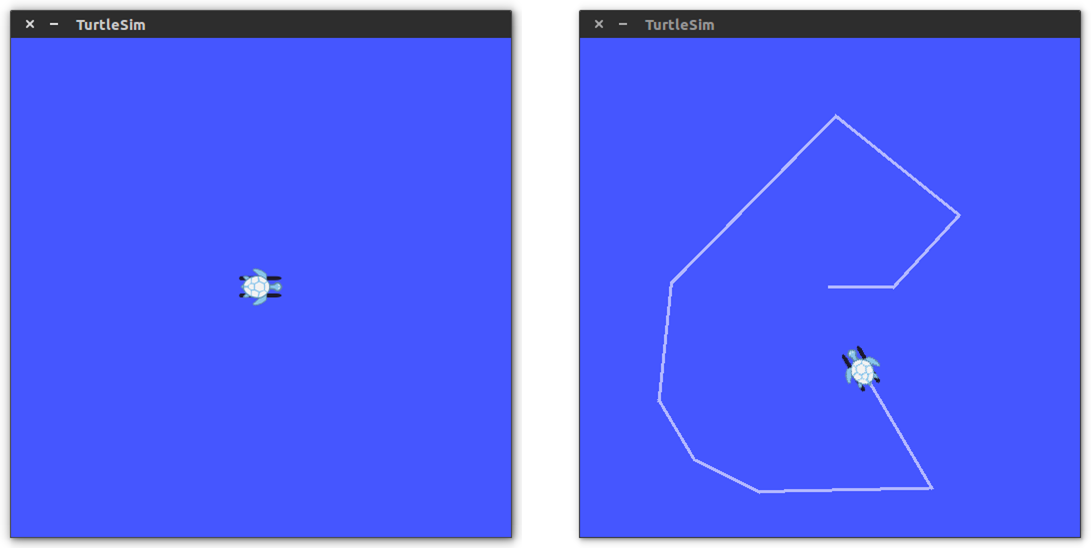
\includegraphics[width=0.9\columnwidth]{pictures/chapter2/pic_02_03.png}
  \caption{turtlesim\_nodeのウィンドウ: (a) 起動時 (b) 亀を移動させた様子}
\end{figure}

turtlesimパッケージのturtle\_teleop\_key実行
別の新しいターミナルウィンドウを開いて、次のコマンドを実行する。

\begin{lstlisting}[language=ROS]
$ rosrun turtlesim turtle_teleop_key
Reading from keyboard
...........................
Use arrow keys to move the turtle.
\end{lstlisting}

これによりメッセージがいくつか表示され、turtlesimパッケージのturtle\_teleop\_key が実行される。turtle\_teleop\_keyを実行したターミナルウィンドウで、キーボードの方向キー(←、→、↑、↓)を押すと、図2-6(b)のように亀が方向キーに応じて動くことが確認できる。これは2つのノード間の通信を利用した簡単な遠隔制御シミュレーションであるが、実際のロボットもこのような方法で遠隔制御することができる。後半の章で、ロボットの遠隔制御について取り上げる。

%-------------------------------------------------------------------------------
\subsubsection{実行中のノードの確認}

rqt\_graphノードは、現在実行中のノードの情報を見ることができるGUI形式のノードである。このrqt\_graphノードを用いて、実行中のノードを確認してみよう。まず、新しいターミナルウィンドウを開いて、次のコマンドを実行する。

\begin{lstlisting}[language=ROS]
$ rosrun rqt_graph rqt_graph
\end{lstlisting}

これにより、rqt\_graphパッケージのrqt\_graphノードが実行され、図2-7のようなグラフが確認できる。
楕円はノード(/teleop\_turtle、/turtlesim)を意味し、四角はトピック(/turtle1/cmd\_vel)を意味する。teleop\_turtle、turtlesim はそれぞれ、turtle\_teleop\_keyノード、turtlesim\_nodeノードの実行名である。外側の3つの四角(teleop\_turtle、turtle1、turtlesim)は異なるグループであることを示している。図2-7を詳細に見てみよう。/teleop\_turtleノードから矢印が引かれて/turtlesimにつながっている。これは、両方のノードが実行中で、両方のノードの間にはトピックメッセージ(/turtle1/cmd\_vel)通信が行われていることを表す。つまり、turtle\_teleop\_keyノードから、ユーザーのキーボードコマンドがロボットのシミュレーターであるturtlesim\_nodeノードに渡されている。ノード間のトピックメッセージ通信については、後半の章で取り上げる。
以上でROS動作テストは完了である。ここまでスムーズに進行した場合、問題無くROSがインストールされている。

\begin{figure}[h]
  \centering
  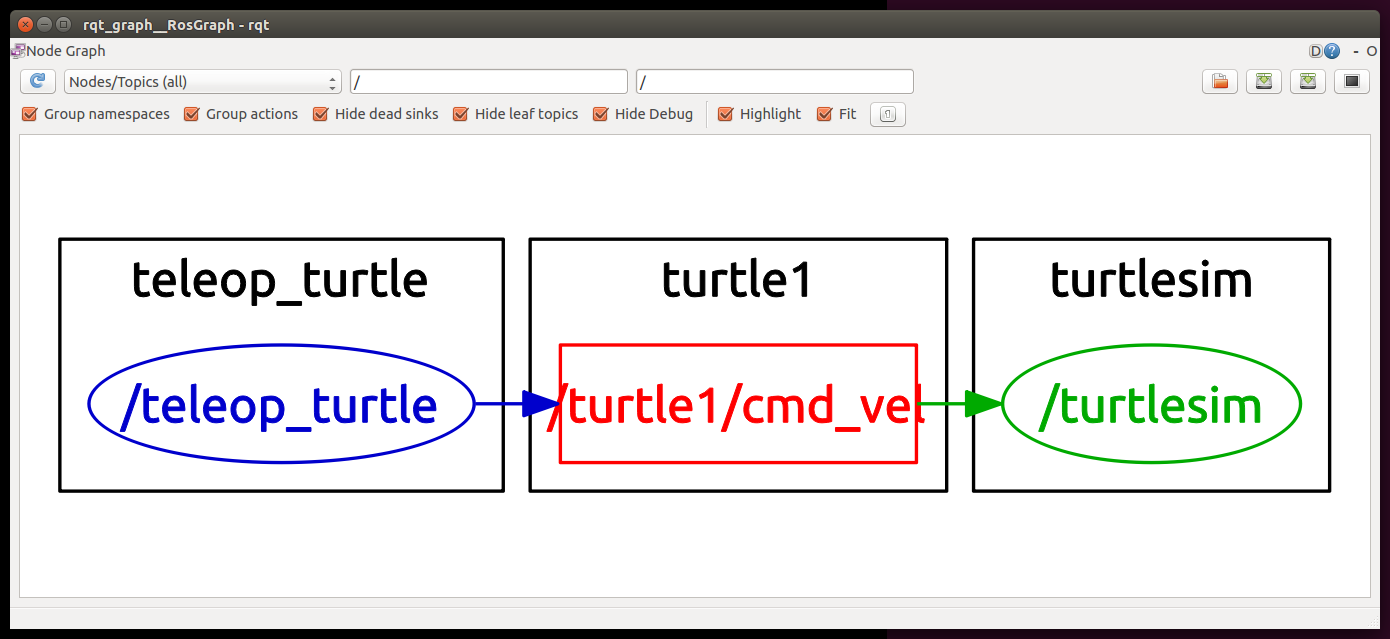
\includegraphics[width=0.9\columnwidth]{pictures/chapter2/pic_02_04.png}
  \caption{rqt\_graphノード}
\end{figure}

%-------------------------------------------------------------------------------
\subsubsection{ノードの終了}
実行されたroscoreとノードを終了する際は、ターミナルウィンドウで<Ctrl>+<c>を押す。

%-------------------------------------------------------------------------------

% !TEX root = ./rosbook_jp.tex
%-------------------------------------------------------------------------------
\chapterimage{chapter_head_3.pdf}

%-------------------------------------------------------------------------------
\chapter{ROSの基本知識}

%-------------------------------------------------------------------------------
\section{ROSで使われる専門用語}
\index{用語}

ROSでは多くの独特の概念や用語が使われる。本節では、頻繁に使用されるROSの用語についてまとめて解説する。ただし、ここですべて理解する必要はなく、わからない用語が出てきても、先に読み進めていただきたい。これらの用語は、実際にROSを利用していけば、自然と身につくものである。

%-------------------------------------------------------------------------------
\subsubsection{マスター(master)}
\index{マスター}\index{Master}

マスター(master)は、ノード間の接続とメッセージ通信の実現に必要なサーバ(ネームサーバ)である。マスターの起動にはroscoreコマンドを用いる。マスターが起動すると、マスターは各ノードの名前を登録し、ノードとの間で必要な情報を送受信する。マスターが起動していなければ、ノード間の接続やメッセージ通信を行うことができない。
マスターは、HTTPベースのプロトコルであるXMLRPCを使用してノードと通信する。XMLRPCでは、マスターとノードは常に接続を維持する必要はなく、ノードは必要な場合にのみマスターに接続して、ノード自身の情報や他のノードの情報をやり取りする。ROSの ノード間通信は、お互いの接続状態を監視していないため、大規模なシステムでも利用できる。また、XMLRPCは計算負荷が小さく、さらに様々なプログラミング言語をサポートしている。

%-------------------------------------------------------------------------------
\subsubsection{ノード(node)}
\index{ノード}\index{Node}

ノード(node)は、ROSの最小の構成要素であり、個々の実行プログラムである。ノードは個別の処理毎に作成され、多くのシステムで繰り返し利用できるように設計される。例えば移動ロボットの場合、センサドライバ、センサデータ処理、障害物検出、モータ駆動、エンコーダ入力、ナビゲーションなど、動作に必要な処理を細分化し、それぞれの処理を実装したノードを組み合わせてシステムを構築する。
ノードを実行する際には、配信者(publisher)、購読者(subscriber)、トピック、サービス名、メッセージの形式、URIアドレスとポートをマスターに登録する。これらの情報を基に、各ノードは、ノード間でトピックメッセージ通信とサービスメッセージ通信を利用して情報を送受信する。
ノードとマスター間の通信にはXMLRPCを利用する。また、ノード同士の通信方式には2種類あり、接続要請と接続応答にはXMLRPCを、メッセージ通信には2点間通信方式であるTCP/IP通信を改良したTCPROSを使用する。すなわち、ノード間の通信はマスターを介して行うわけではない。ノードのURIアドレスには、ノードを実行しているPCのROS\_HOSTNAME変数を使用し、ポートは任意の値に設定される。

%-------------------------------------------------------------------------------
\subsubsection{パッケージ(package)}
\index{パッケージ}\index{Package}

ROSのアプリケーションはパッケージ(package)単位で開発される。ROS Indigoは201 5年5月20日現在、約1,660個(http://www.ros.org/debbuild/indigo.html)のパッケージを提供しており、また、ユーザーが開発し公開したパッケージは約5,400個\footnote{\url{http://rosindex.github.io/stats/}}にもなる。

%-------------------------------------------------------------------------------
\subsubsection{メタパッケージ(metapackage)}
\index{メタパッケージ}\index{Metapackage}

メタパッケージ(metapackage)は、共通の目的を持ったパッケージを集めたパッケージのセットである。

%-------------------------------------------------------------------------------
\subsubsection{メッセージ(Message)}
\index{メッセージ}\index{Message}

メッセージ(message、msg)とは、ノード間でやり取りされる情報である。メッセージは整数型、浮動小数点型、論理型などの変数で構成されている。また、この他にもユーザーが自由にメッセージの型を設定でき、例えば配列型やネスト構造(他のファイルで宣言されたメッセージ型を内包したメッセージ型)なども使用できる。メッセージを利用した通信方法には、一方向のメッセージ送受信方式であるトピック(topic)メッセージ通信と、双方向のメッセージ送受信方式であるサービス(service)メッセージ通信がある。

%-------------------------------------------------------------------------------
\subsubsection{トピック(Topic)}
\index{トピック}\index{Topic}

トピック(topic)は一方向で非同期方式のメッセージ送受信方式である。配信者(publisher)が配信したいデータをもつとき、そのデータを変数として含むメッセージに固有のトピック名を付けてマスターに登録する。その後、このトピックの受信を希望する購読者(subscriber)は、登録されたトピック名に対応する配信者の情報をマスターから受け取る。この情報に基づいて,購読者は配信者と直接接続して、メッセージをトピックで送受信する。

%-------------------------------------------------------------------------------
\subsubsection{配信および配信者(publish and publisher)}
\index{配信}\index{Publish}\index{配信者}\index{Publisher}

配信(publish)とは、各トピックで定義されたメッセージを送信することをいう。配信者(publisher)は、メッセージを配信するために、トピック名などの情報をマスターに登録する。トピックを購読したい購読者は、マスターから必要な情報を得て配信者と接続し、メッセージを受け取る。一つのノードは複数の配信者を利用できる。以降では、配信者を実行するノードを「配信者ノード」と呼ぶ。

%-------------------------------------------------------------------------------
\subsubsection{購読および購読者(subscribe and subscriber)}
\index{購読}\index{Subscribe}\index{購読者}\index{Subscriber}

購読(subscribe)とは、各トピックで定義されたメッセージを受信することをいう。購読者(subscriber)は、トピック名などの情報をマスターに登録し、購読しようとするトピックの配信者の情報をマスターから受ける。この情報に基づいて購読者は、配信者と直接接続してメッセージを受け取る。一つのノードで複数の購読者を利用できる。以降では、購読者を実行するノードを「購読者ノード」と呼ぶ。

%-------------------------------------------------------------------------------
\subsubsection{サービス(service)}
\index{サービス}\index{Service}

サービス(service)とは、メッセージ同期方式の通信方式である。上述した配信と購読に基づくトピックメッセージ通信方式は非同期方式であり、データの送受信を効率的に行うことができる。また、一度接続処理を行えば、その後は連続的にメッセージを送受信できるので、継続してメッセージを送信しなければならないセンサデータの通信処理に適している。しかし、場合によっては、リクエスト(request)とレスポンス(response)によって構成される、同期方式のメッセージ交換方式も必要となる。ROSは、これをサービスメッセージ通信と呼ぶ通信方式で提供する。サービスメッセージ通信は、リクエストを受け取ると情報を送信するサービスサーバ(service server)と、リクエストを送信し情報を受け取るサービスクライアント(service client)から構成される。サービスは、トピックとは異なり、一回限りのメッセージ通信である。サービスのリクエストとレスポンスが完了すると、二つのノードの接続は一度切断される。

%-------------------------------------------------------------------------------
\subsubsection{サービスサーバ(service server)}
\index{サービスサーバ}\index{Service Server}

サービスサーバ(service server)は、リクエストを入力として受け取り、レスポンスを出力するサービスメッセージ通信のサーバである。リクエストとレスポンスはメッセージであり、サービスサーバはリクエストを受信すると、指定されたサービスを実行し、その結果をサービスクライアントに送信する。通常、サービスサーバは、決められた命令を受けて、特定の処理を実行するノードで使用される。

%-------------------------------------------------------------------------------
\subsubsection{サービスクライアント(service client)}
\index{サービスクライアント}\index{Service Client}

サービスクライアント(service client)は、リクエストを出力し、レスポンスを受け取るサービスメッセージ通信のクライアントである。リクエストとレスポンスはメッセージであり、サービスクライアントはリクエストをサービスサーバに送信し、そのレスポンスを受信する。サービスクライアントは、ある定められたコマンドをサービスサーバへ送信し、結果を受けるノードで使用される。

%-------------------------------------------------------------------------------
\subsubsection{catkinビルドシステム(catkin build system)}
\index{ビルドシステム}\index{Build System}\index{Catkin}

catkin(キャッキン)はROSのビルドシステムである。catkinビルドシステムは、一般的なビルドシステムであるCMake(Cross Platform Make)を拡張したものであり、CMakeと同様に、パッケージのフォルダ内のCMakeLists.txtファイルにビルド環境を記述している。catkinはROS Fuerteバージョンからアルファテストを開始して、Groovyでコアパッケージがcatkinビルドシステムに切り代わり、Hydroバージョン以降は全システムで使えるようになった。catkinビルドシステムを用いると、パッケージのビルド、パッケージ管理、依存関係パッケージの自動インストールなどが容易に行える。

%-------------------------------------------------------------------------------
\subsubsection{ROSビルドシステム(rosbuild system)}
\index{ビルドシステム}\index{Build System}

ROSビルド(rosbuild)はcatkinビルドシステム以前に使用されたビルドシステムであり、今も一部のユーザーが使用している。しかしROSのバージョンの互換性のために残されたものであり、今後は使用されないため、本書ではrosbuildの使用は推奨しない。もし、rosbuildビルドシステムを使用した以前のパッケージを使用する必要がある場合、catkinビルドシステムへの修正を試みるべきである。

%-------------------------------------------------------------------------------
\subsubsection{roscore}
\index{roscore}

roscoreはROSマスターを実行するためのコマンドである。同じネットワークセグメントであれば、どのPCで実行してもよい。ただし、マルチROSマスターをサポートしている場合を除いては、roscoreは同じネットワーク内で1つのみ実行できる。ノードを起動する際には、ネットワーク内の1台のPCで必ずマスターを起動しておく必要がある。またユーザーは、ノードを実行するネットワーク内のすべてのPCで、マスターが実行されているPCのURIやIPアドレス、ポート番号を、「~/.bashrc」ファイルのROS\_MASTER\_URI変数に設定しておかなければならない。ROS\_MASTER\_URI変数が設定されていない場合は、ノードを実行したPCのIPアドレスと11311ポートが使用される。

%-------------------------------------------------------------------------------
\subsubsection{パラメータ(parameter)}
\index{パラメータ}\index{Parameter}

パラメータ(parameter)とは、ノード内で使用され、ノード実行中に変更可能な変数である。パラメータは規定値が設定されており、ノード実行中に外部からの読み取り、または書き込みができる。例えば、外部デバイスを接続したUSBポートの番号やカメラキャリブレーション値、モータの速度やコマンドの最大値と最小値などをノード実行中に外部から確認することや、値を変更することができる。

%-------------------------------------------------------------------------------
\subsubsection{パラメータサーバ(parameter server)}
\index{パラメータサーバ}\index{Parameter Server}

パラメータサーバ(parameter server)とは、ノードでパラメータを使用する際、パラメータの書き込みや読み込みを行うサーバである。パラメータサーバは、マスターの起動と同時に自動的に立ち上がる。エンコード形式にはXMLを採用し、伝送方式にはリクエスト/レスポンス方式のHTTPプロトコルであるXMLRPCを使用する。

%-------------------------------------------------------------------------------
\subsubsection{rosrun}
\index{rosrun}

rosrunはROSにおける最も基本的な実行コマンドである。パッケージ内の1つのノードを実行する際に使用する。

%-------------------------------------------------------------------------------
\subsubsection{roslaunch}
\index{roslaunch}

rosrunが1つのノードを実行するコマンドであるのに対し、roslaunchは複数のノードを実行するコマンドである。さらにパッケージのパラメータやノード名の変更、ノードのNamespaceの設定、ROS\_ROOTとROS\_PACKAGE\_PATHの設定、環境変数の変更など、多くのオプションを備えたROSコマンドである。roslaunchは「.launch」という拡張子のファイルを使用して、実行ノードの設定ができる。roslaunchの形式はXMLに基づいており、XMLタグ形式でオプションを設定する。

%-------------------------------------------------------------------------------
\subsubsection{bag}
\index{Bag}\index{rosbag}

ROSで送受信されるメッセージのデータをファイルとして保存する際の形式がbagである。「.bag」という拡張子を使う。ROSは、bagとして保存したメッセージを後に必要に応じて再生することで、実行時の状況をそのまま再現できる。たとえば、センサーを利用したロボットの走行実験を行うとき、bagを使用してセンサーのデータをメッセージの形式で保存する。その後、保存しておいたbagファイルを再生することで、実際にロボットを走行させなくても、実験時のセンサーの値を繰り返し使用できる。このbagの記録・再生の機能を活用すれば、プログラムの修正が多い複雑なアルゴリズムの開発を効率化できる。

%-------------------------------------------------------------------------------
\subsubsection{ROS Wiki}
\index{ROS Wiki}

ROSの各パッケージと機能を説明するページ(http://wiki.ros.org/)である。このページには各パッケージの簡単な説明、使用されるパラメータ、著作者、ライセンス、ホームページ、リポジトリ、チュートリアルなどが記載されている。

%-------------------------------------------------------------------------------
\subsubsection{リポジトリ(repository)}
\index{リポジトリ}\index{Repository}

リポジトリ(repository)は、パッケージが格納されているウェブ上のURLアドレスで、svn、hg、gitなどのソース管理システムを利用して、障害情報、開発記録、ソースコードのダウンロードなどを管理している。公開されたパッケージでは、各パッケージのWikiにリポジトリを記載している。

%-------------------------------------------------------------------------------
\subsubsection{rqtグラフ(rqt\_graph)}
\index{グラフ}\index{rqt\_graph}\index{rqt}

rqt\_graph(rqt\_graph)は、ノード、トピック、配信者、購読者の関係を視覚的にわかりやすく表示するツールである。実行コマンドはrqt\_graph、あるいはrosrun rqt\_graph rqt\_graphであり、両者に違いはない。なお、これらは実行中のトピックメッセージ通信をグラフ形式で表示するものであり、通信が一度しか行われないサービスメッセージ通信は表示できない。

%-------------------------------------------------------------------------------
\subsubsection{名前(name)}
\index{名前}\index{Name}

ノード、パラメータ、トピック、サービスには、すべて固有の名前(name)が付けられている。各ノードでパラメータ、トピック、サービスを利用するときには、マスターに登録された名前に基づいて、他のノードの検索、接続、メッセージ送受信を行う。また、名前は起動時に変更でき、同じノード、パラメータ、トピック、サービスであっても別の名前で登録すれば重複して使用できるなど、極めて柔軟である。

%-------------------------------------------------------------------------------
\subsubsection{クライアントライブラリ(client library)}
\index{クライアントライブラリ}\index{Client Library}

ROSは、特定のプログラミング言語にできるだけ依存しないように、クライアントライブラリ(client library)として、各種の言語による開発環境を提供している。主な言語には、C ++、Python、Lispなどがあり、さらにjava、lua、.NET、EusLisp、Rなどの言語も使用できる。クライアントライブラリは、これまでroscpp、rospy、roslisp、rosjava、roslua、roscs、roseus、PhaROS、rosRなどが開発されている。

%-------------------------------------------------------------------------------
\subsubsection{TCPROS}
\index{TCPROS}

メッセージとサービスで使用されるTCP/IPベースのメッセージ伝送方式である。

%-------------------------------------------------------------------------------
\subsubsection{UDPROS}
\index{UDPROS}

メッセージとサービスで使用されるUDPベースのメッセージ伝送方式である。あまり使用されない。

%-------------------------------------------------------------------------------
\subsubsection{CMakeLists.txt}
\index{CMakeLists.txt}

ROSのビルドシステムであるcatkinはCMakeを拡張したものである。パッケージフォルダ内のCMakeLists.txtファイルにビルド環境を記述している。

%-------------------------------------------------------------------------------
\subsubsection{package.xml}
\index{package.xml}

パッケージの情報を記載したXMLファイルである。パッケージの名前、著作者、ライセンス、依存性パッケージなどが記載されている。

%-------------------------------------------------------------------------------
\section{メッセージ通信}
\index{メッセージ}\index{Message}

本節では、ROSの重要な機能であるノード間のメッセージ通信\footnote{\url{http://wiki.ros.org/ROS/Concepts}}\footnote{\url{http://wiki.ros.org/ROS/Higher-Level\%20Concepts}}について説明する。作業目的に応じて細分化されたノードは、他のノードと処理結果を送受信(メッセージ通信)することで一つの大きなプログラムになる。ノード間のメッセージ通信には、トピックメッセージ通信とサービスメッセージ通信の2つの方法がある。これらの通信方法について、以下で詳しく見ていこう。

%-------------------------------------------------------------------------------
\subsection{トピックメッセージ通信}
\index{トピックメッセージ}\index{Topic}

トピックメッセージ通信は、図3-1のように、情報を送信する配信者と情報を受信する購読者が、トピックと呼ばれる形式でメッセージを送受信するものである。一つの配信者から複数の購読者への通信や、逆に複数の配信者から一つの購読者への通信も可能である。もちろん、一つの配信者から一つの購読者や、多数の配信者から多数の購読者への通信も可能である。トピックメッセージ通信は、例えば移動ロボットの両輪のエンコーダ値を計測して、ロボットの現在位置であるオドメトリ(odometry)情報を計算し、得られた位置情報をトピックメッセージ(x、y、θ)として送信する場合など、一方向で連続的なメッセージの送受信に用いられる。

\begin{figure}[h]
  \centering
  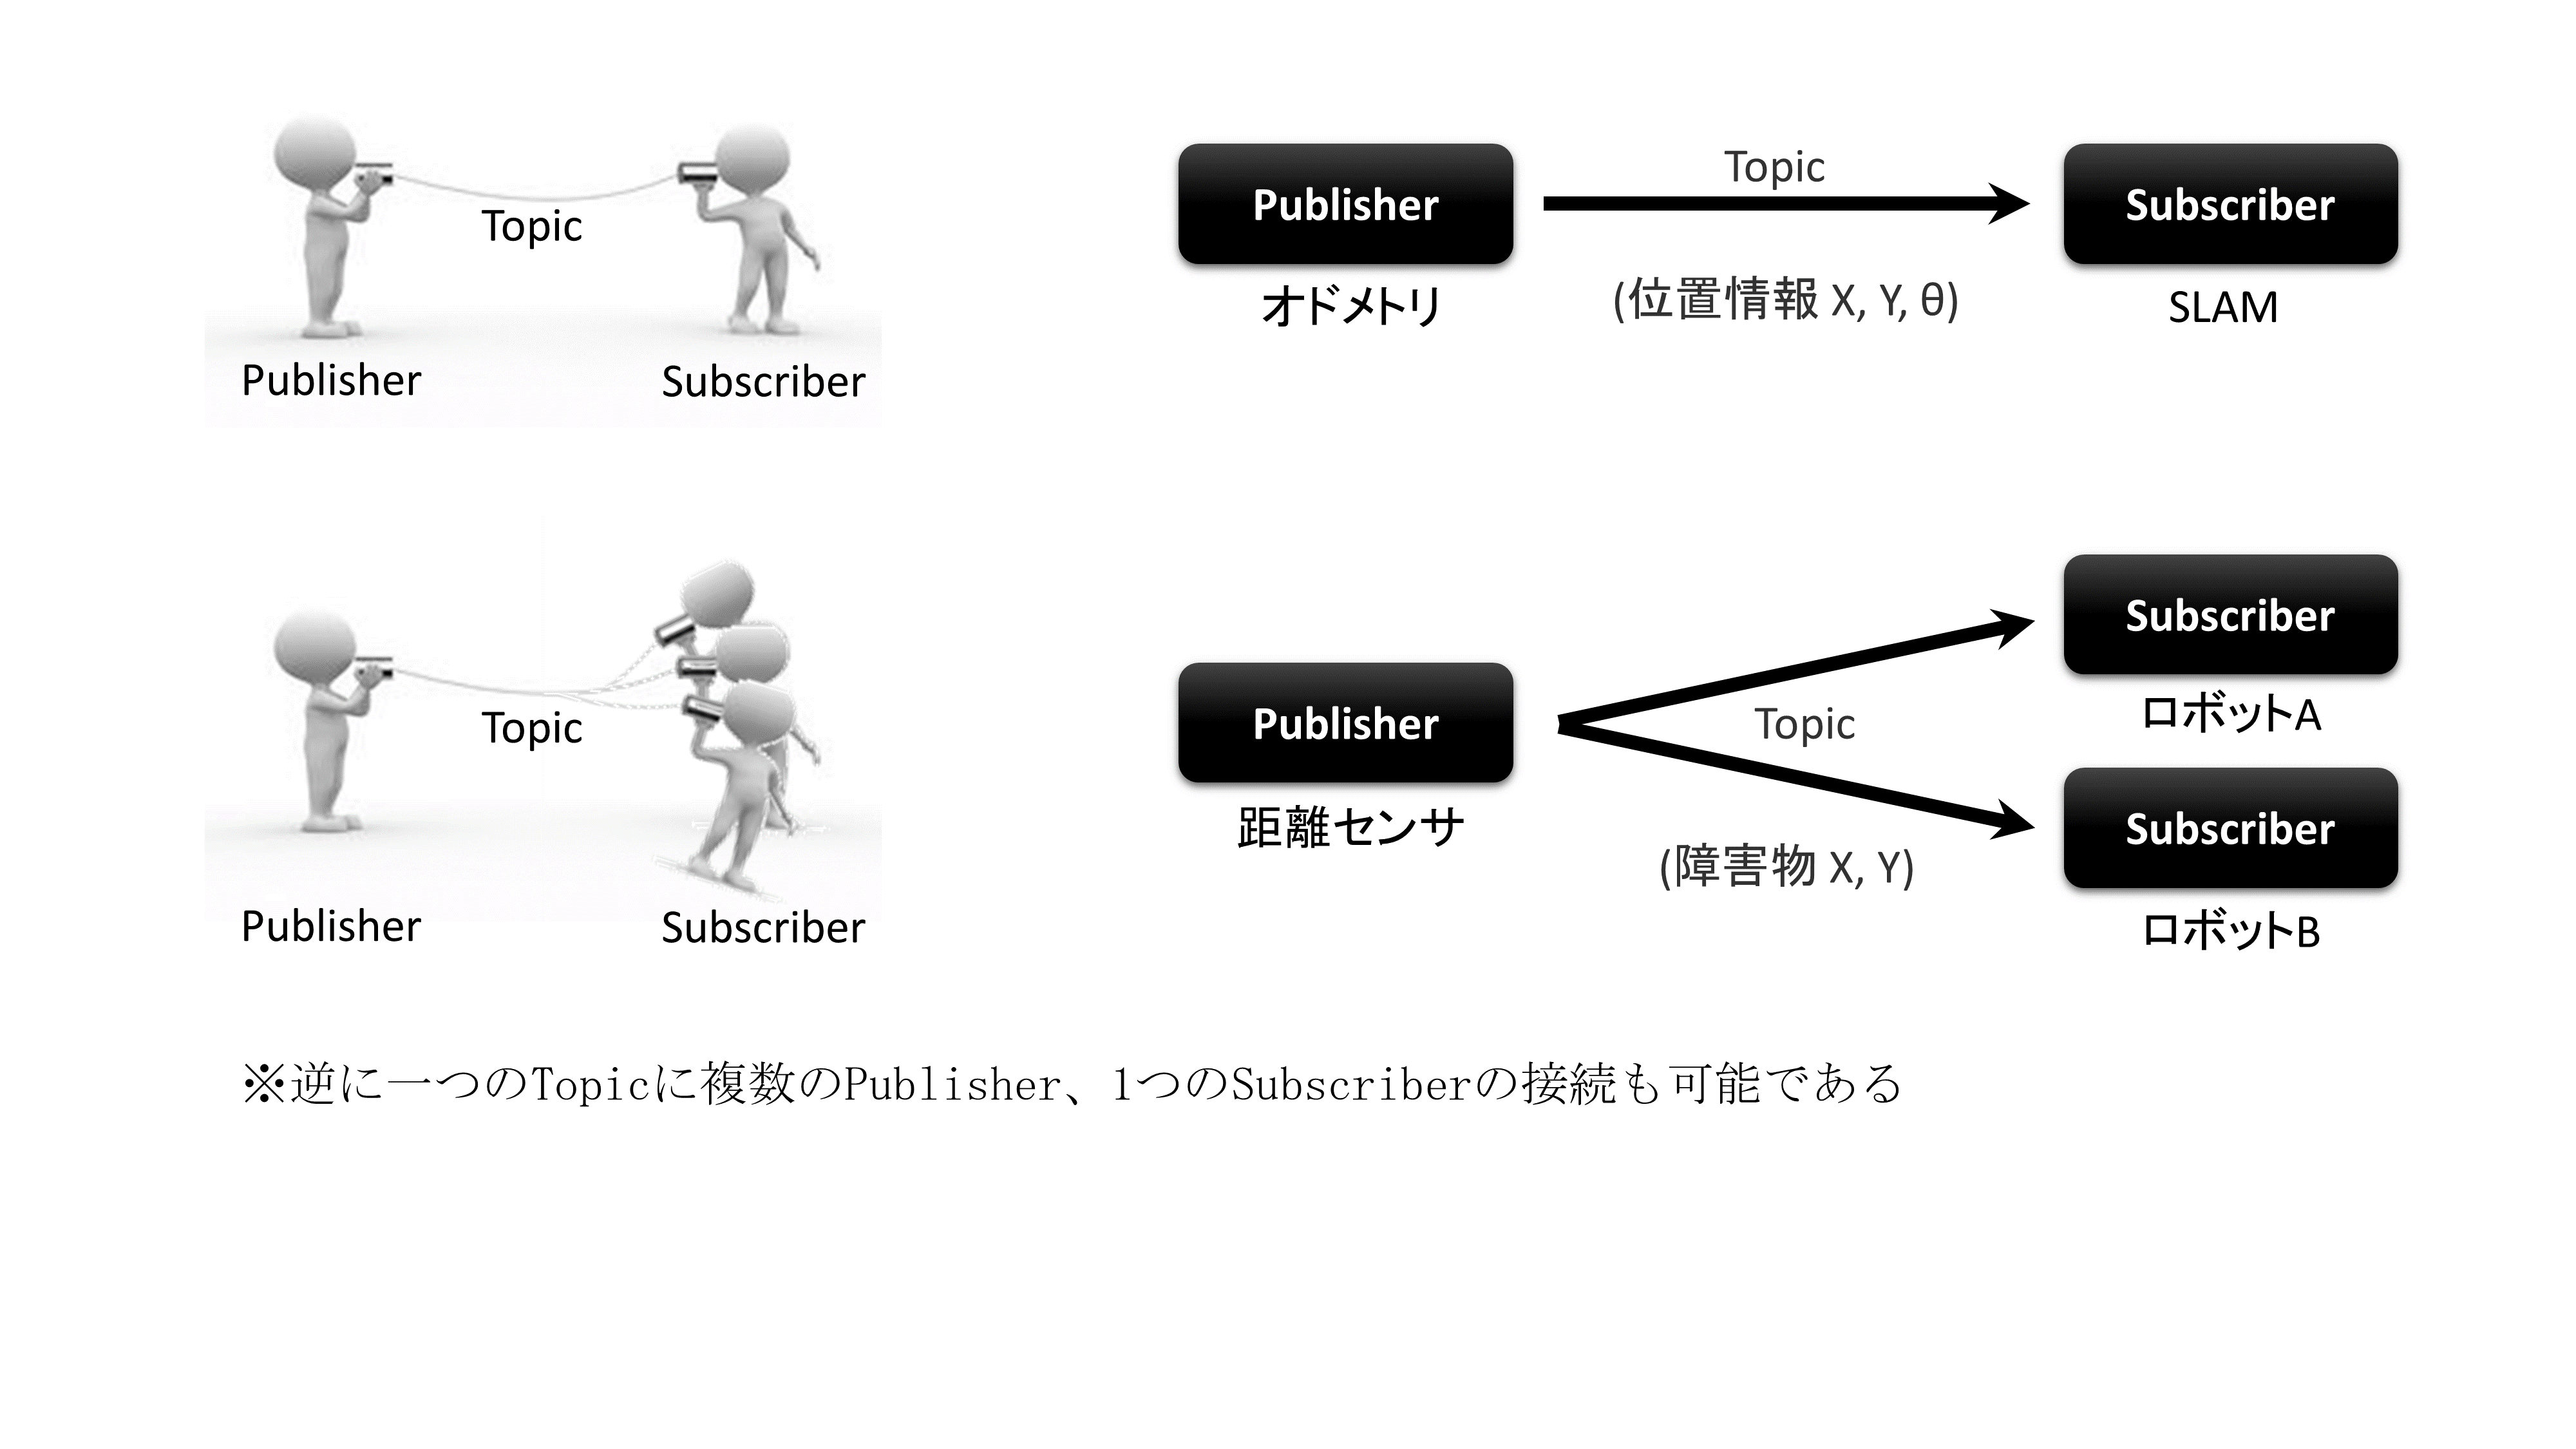
\includegraphics[width=12cm]{pictures/chapter3/pic_03_01.png}
  \caption{トピックメッセージ通信}
\end{figure}

%-------------------------------------------------------------------------------
\subsection{サービスメッセージ通信}
\index{サービス}\index{Service}\index{Request}\index{Response}\index{Response}\index{Service Client}\index{Service Server}
サービスメッセージ通信とは、図3-2に示すようにサービスをリクエスト(request)するサービスクライアント(service client)と、レスポンス(response)を返すサービスサーバ(service server)間の、双方向サービスメッセージ通信である。例えば、図3-2に示すように、クライアントがサーバに現在時刻をリクエストすると、サーバは時間を調べてクライアントにレスポンスを返す。このサービスメッセージ通信は、トピックメッセージ通信とは異なり、一対一の通信のみが可能である。

\begin{figure}[h]
  \centering
  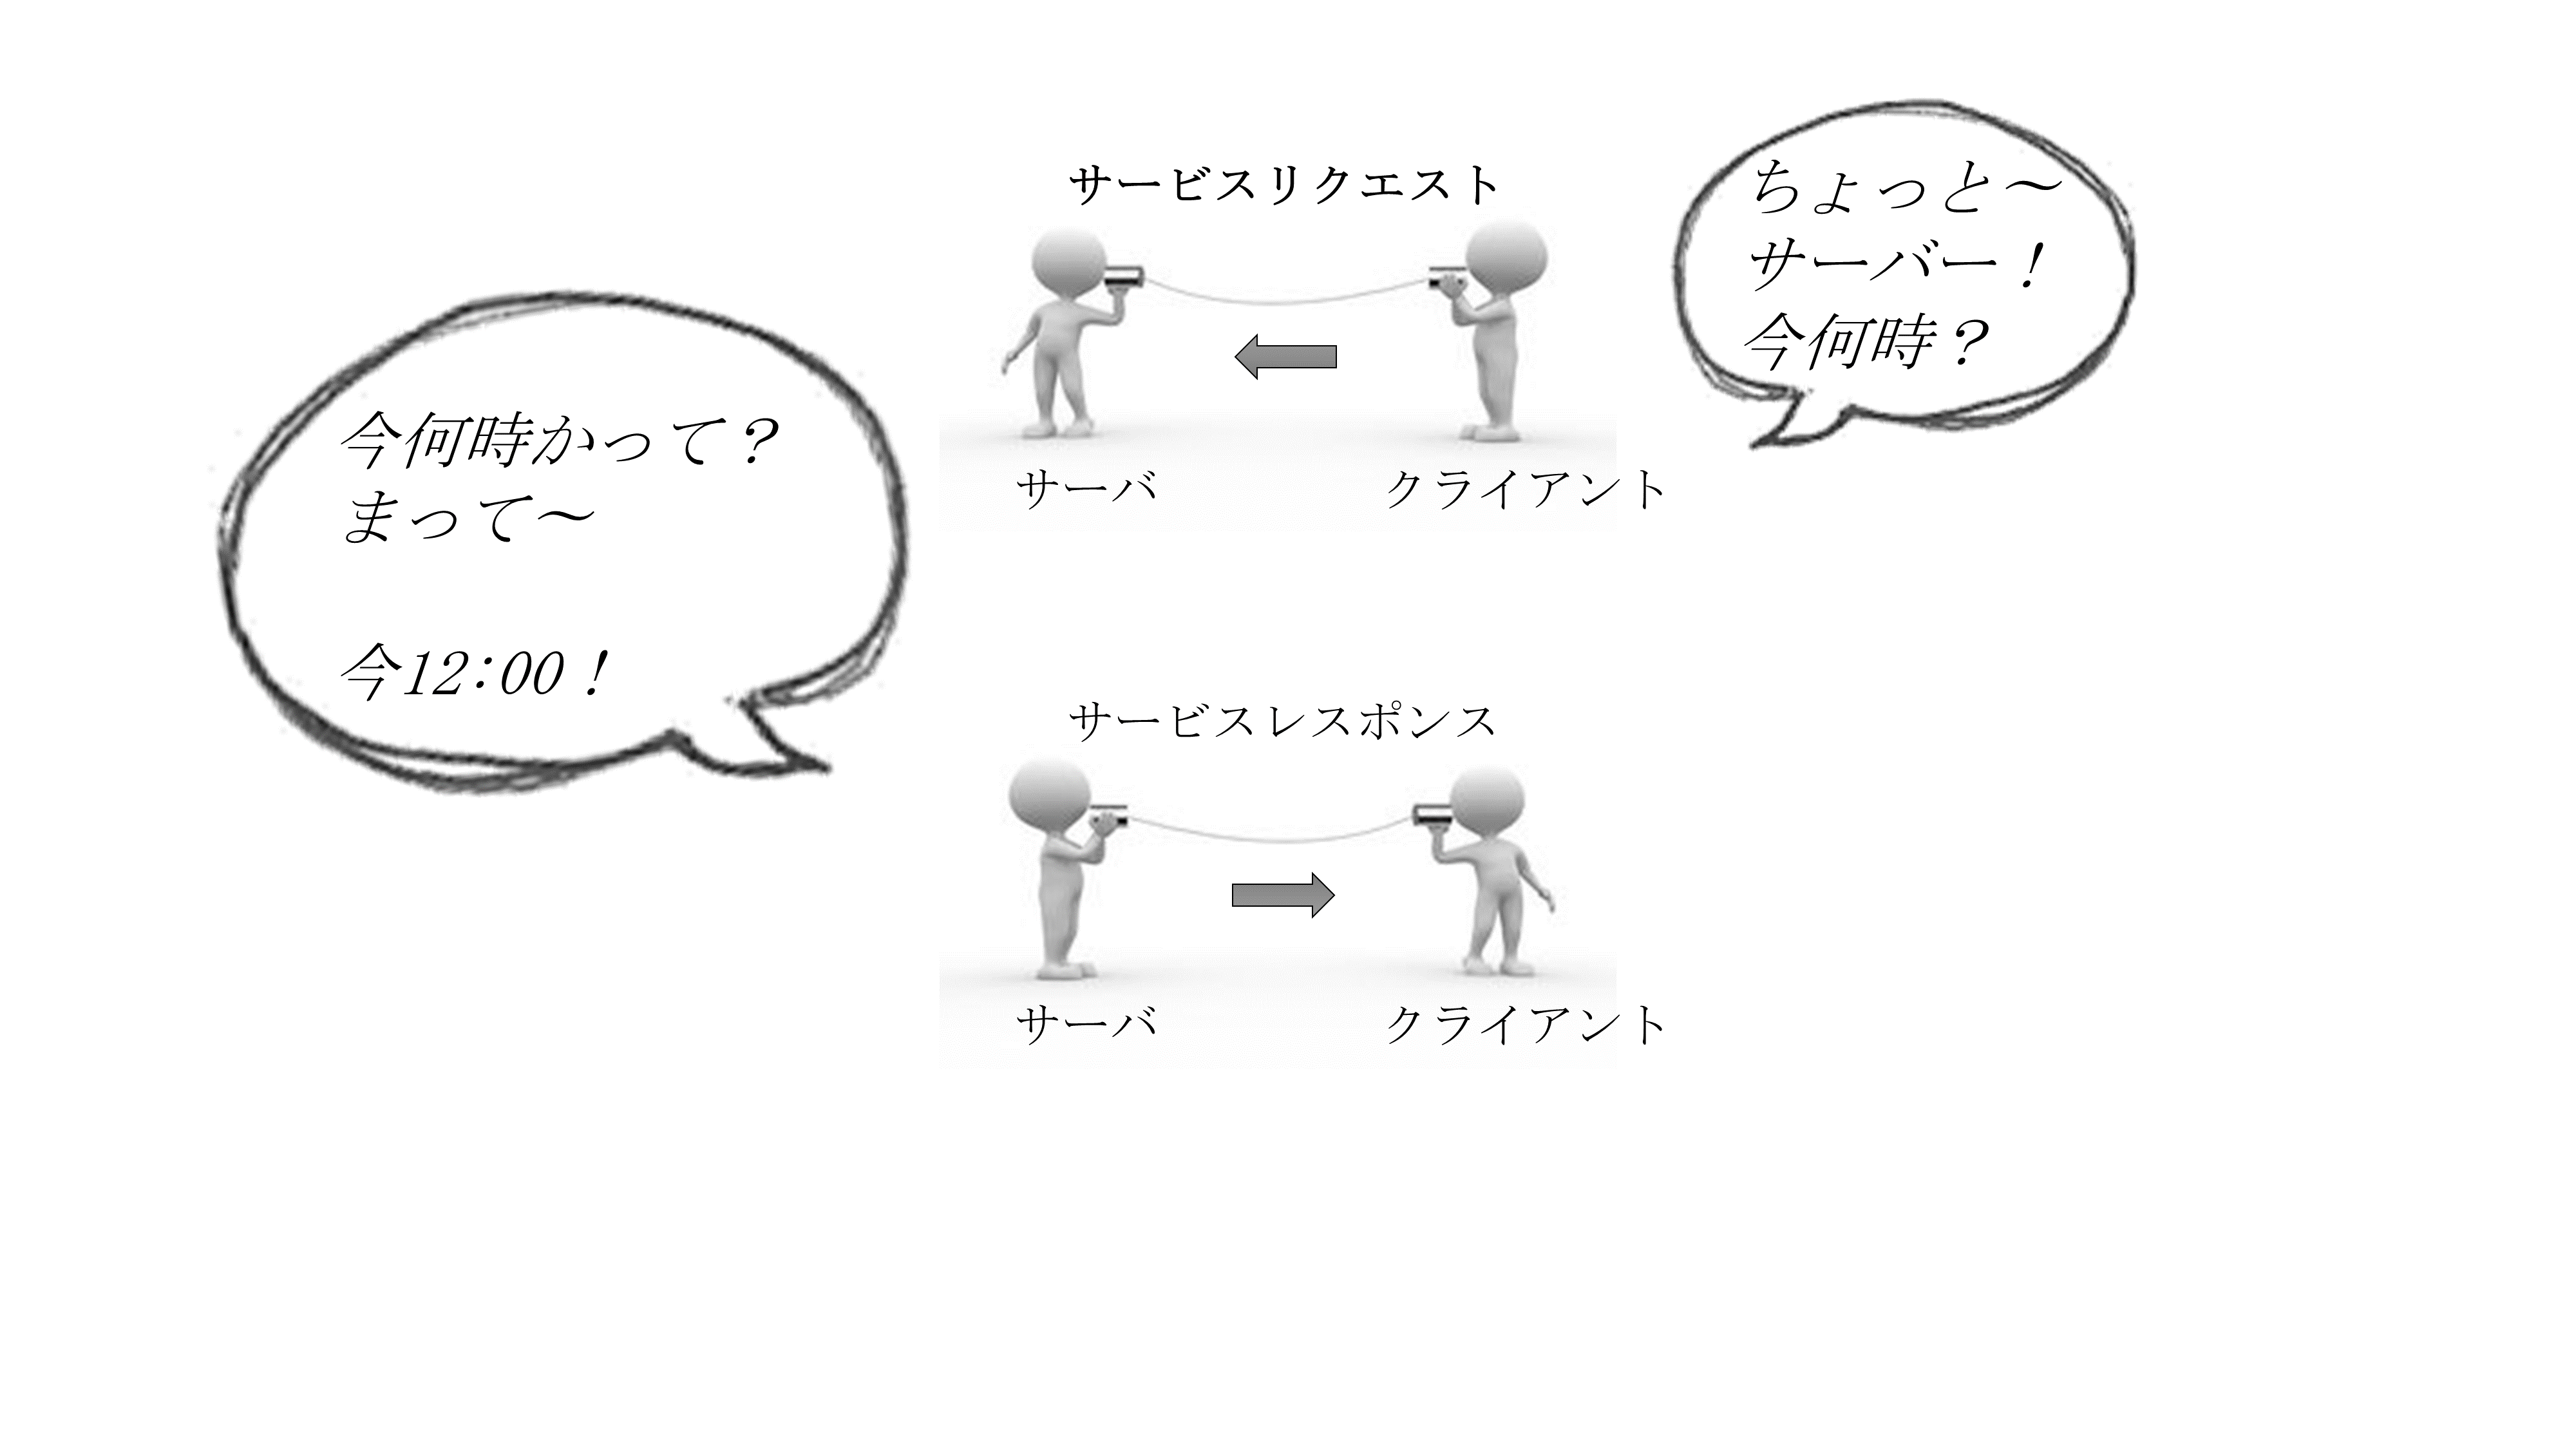
\includegraphics[width=12cm]{pictures/chapter3/pic_03_02.png}
  \caption{サービスメッセージ通信}
\end{figure}

%-------------------------------------------------------------------------------
\subsection{マスターによる接続管理}
\index{マスター}\index{Master}

配信者、購読者、サービスサーバ、サービスクライアントは、一般にそれぞれ異なるノードの中に存在する。従って、これらのノードがメッセージ通信をするには、ノードを接続する必要がある。このノード間の接続を管理するのがマスター\footnote{\url{http://wiki.ros.org/Master}}である。マスターは、ノードの名前、トピックやサービスの名前、URIアドレスとポート、パラメータなどの情報を管理している。ノードは、生成と同時にマスターに情報を登録し、マスターを介して接続先のノードの情報を得る。その後、ノードとノードが直接接続してメッセージ通信を行う。
図3-3にノード間のメッセージ通信の仕組みを示す。

\begin{figure}[h]
  \centering
  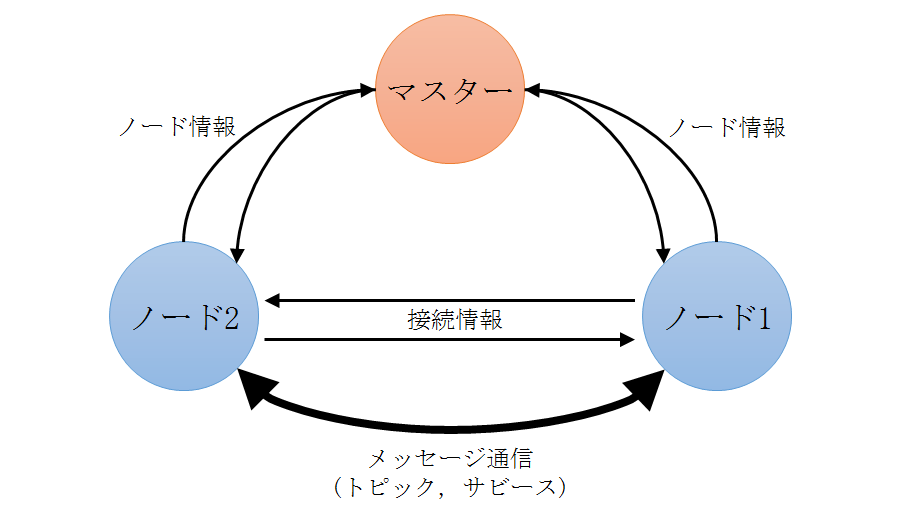
\includegraphics[width=12cm]{pictures/chapter3/pic_03_03.png}
  \caption{メッセージ通信}
\end{figure}

マスターは、ノードの情報を管理し、各ノードは、必要に応じて他のノードと接続、メッセージ通信を行う。以下では、最も重要なマスター、ノード、トピック\footnote{\url{http://wiki.ros.org/Topics}}、サービス\footnote{\url{http://wiki.ros.org/Services}}、メッセージ\footnote{\url{http://wiki.ros.org/Messages}}間の処理の流れについて、より詳しく説明する。

%-------------------------------------------------------------------------------
\subsection{マスターの実行}
\index{マスター}\index{Master}

ROSの通信の使用にあたり、ノード間のメッセージ通信の接続情報を管理するマスターを最初に実行する必要がある。ROSマスターは、roscoreコマンドにより実行され、リモートプロシージャコール(RPC)の一種であるXMLRPCを用いてサーバを動作させる。マスターは、ノード間の接続のために、ノードの名前、トピックとサービスの名前、メッセージの形式、URIアドレスとポートを登録し、他のノードから問い合わせがあったときに、必要なノードの情報を送信する。

\begin{lstlisting}[language=ROS]
$ roscore
\end{lstlisting}

\begin{figure}[h]
  \centering
  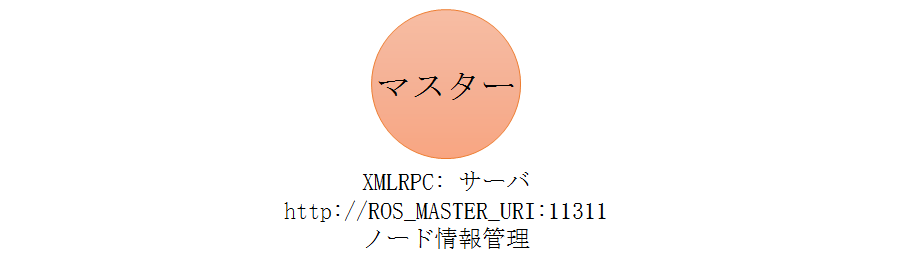
\includegraphics[width=12cm]{pictures/chapter3/pic_03_04.png}
  \caption{マスターのみを起動した状態}
\end{figure}

%-------------------------------------------------------------------------------
\subsection{購読者(subscriber node)の実行}
\index{購読者}\index{Subscriber}

購読者ノードは、rosrun又はroslaunchコマンドにより実行される。購読者ノードは、実行時に、マスターに自分の購読者ノード名、購読しようとするトピック名、メッセージの形式、URIアドレスとポートを登録する。この時、図3-5のように、マスターと購読者ノードはXMLRPCを利用して通信する。

\begin{lstlisting}[language=ROS]
$ rosrun PACKAGE_NAME NODE_NAME
$ roslaunch PACKAGE_NAME LAUNCH_NAME
\end{lstlisting}

\begin{figure}[h]
  \centering
  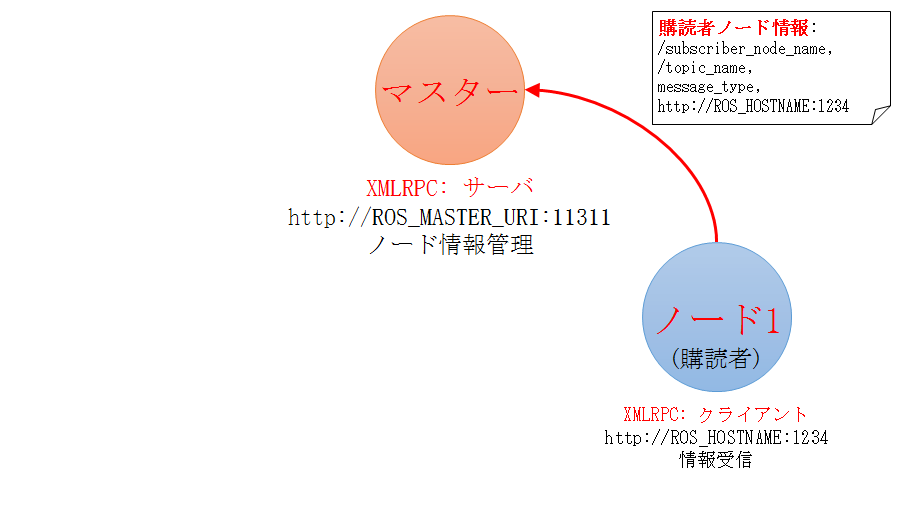
\includegraphics[width=12cm]{pictures/chapter3/pic_03_05.png}
  \caption{購読者ノードの実行}
\end{figure}

%-------------------------------------------------------------------------------
\subsection{配信者ノード(publisher node)の実行}
\index{配信者}\index{Publisher}

配信者ノードは、購読者ノードと同様に、rosrun又はroslaunchコマンドにより実行される。配信者ノードは、実行時に、マスターに自分の配信者ノード名、配信しようとするトピック名、メッセージの形式、URIアドレスとポートを登録する。この時、図3-6のように、マスターと配信者ノードはXMLRPCを利用して通信する。

\begin{figure}[h]
  \centering
  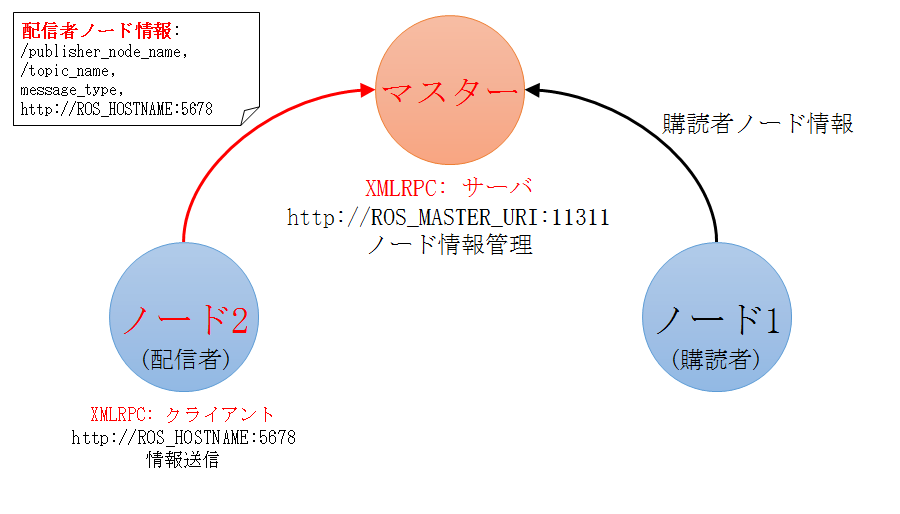
\includegraphics[width=12cm]{pictures/chapter3/pic_03_06.png}
  \caption{配信者ノードの実行}
\end{figure}

%-------------------------------------------------------------------------------
\subsection{購読者ノードへの配信者情報の通知}
\index{購読者}\index{Subscriber}

マスターは、購読者ノードに購読者が接続したい配信者ノード名やトピック名などの情報を送信する。図3-7のように、マスターと購読者ノードはXMLRPCを利用して通信する。

\begin{figure}[h]
  \centering
  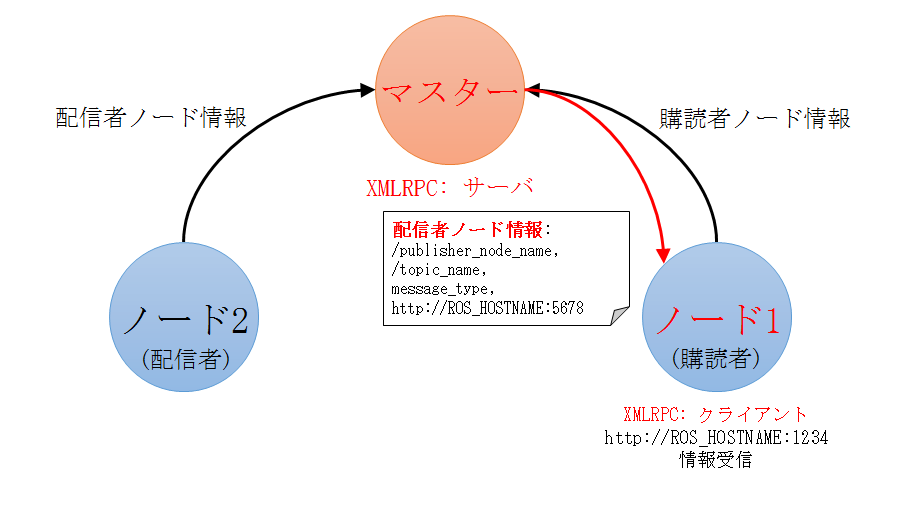
\includegraphics[width=12cm]{pictures/chapter3/pic_03_07.png}
  \caption{購読者へ配信者ノードへの情報の通知}
\end{figure}

%-------------------------------------------------------------------------------
\subsection{購読者ノードの接続要請}
\index{購読者}\index{Subscriber}

購読者ノードは、マスターから受信した配信者の情報に基づいて、配信者ノードに直接接続を要請する。この時に送信される情報には、自分の購読者ノード名、トピック名、メッセージ方式が含まれる。図3-8のように、配信者ノードと購読者ノードはXMLRPCを利用して通信する。

\begin{figure}[h]
  \centering
  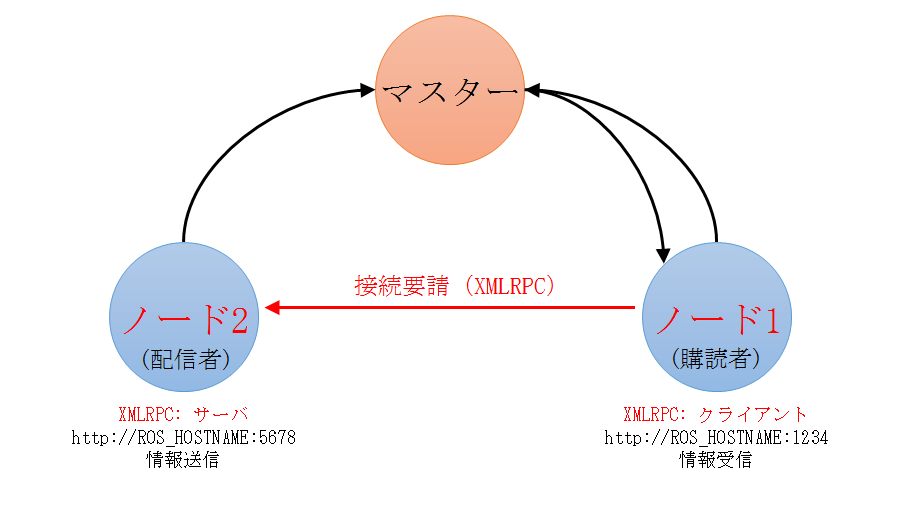
\includegraphics[width=12cm]{pictures/chapter3/pic_03_08.png}
  \caption{配信者ノードに接続要請}
\end{figure}

%-------------------------------------------------------------------------------
\subsection{配信者ノードの接続応答}
\index{配信者}\index{Publisher}

配信者ノードは、購読者ノードの接続要請への応答として、自身のURIアドレスとポートを送信する。図3-9のように、配信者ノードと購読者ノードはXMLRPCを利用して通信する。

\begin{figure}[h]
  \centering
  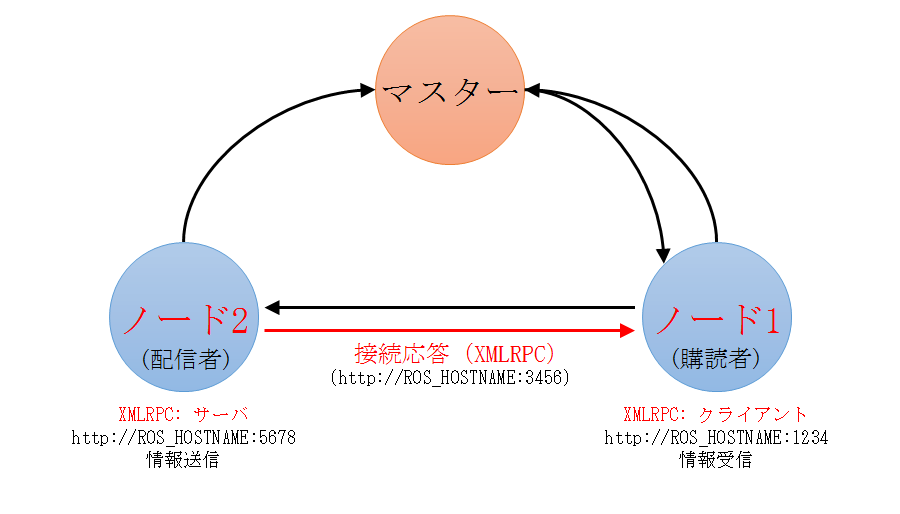
\includegraphics[width=12cm]{pictures/chapter3/pic_03_09.png}
  \caption{配信者ノードの接続応答}
\end{figure}

%-------------------------------------------------------------------------------
\subsection{TCP接続}
\index{TCPROS}

購読者ノードはTCPROSを用いて、配信者ノードに対するクライアントを生成し、配信者ノードと直接接続する。図3-10のように、購読者ノードと配信者ノード間はTCP/IP方式であるTCPROSを利用して通信する。

\begin{figure}[h]
  \centering
  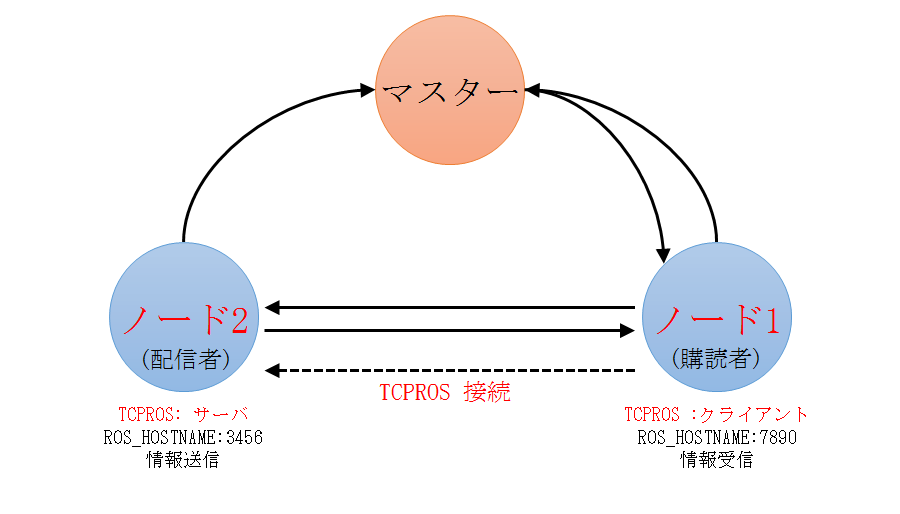
\includegraphics[width=12cm]{pictures/chapter3/pic_03_10.png}
  \caption{購読者ノードと配信者ノードの接続}
\end{figure}

%-------------------------------------------------------------------------------
\subsection{トピックメッセージの送信}
配信者ノードは、購読者ノードにトピックメッセージを送信する。ノード間の通信は、TCPROSを使用する。

\begin{figure}[h]
  \centering
  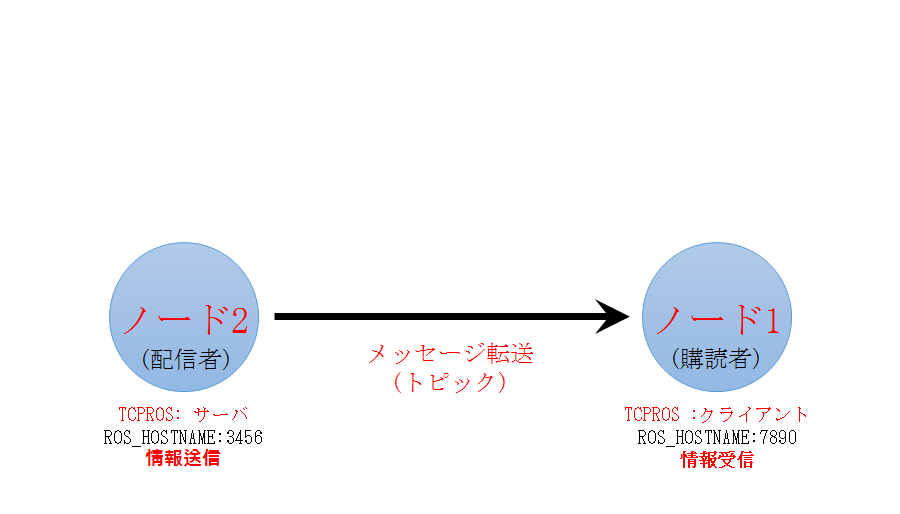
\includegraphics[width=12cm]{pictures/chapter3/pic_03_11.png}
  \caption{トピックメッセージ通信}
\end{figure}

%-------------------------------------------------------------------------------
\subsection{サービスクライアントとサービスサーバによるサービスメッセージ通信}
\index{サービス}\index{Service}\index{Request}\index{Response}\index{Response}\index{Service Client}\index{Service Server}

ここまでは、メッセージ通信のうち、トピックメッセージ通信について学んだ。トピックメッセージ通信では、配信者や購読者が停止していなければ、メッセージを連続して配信し、購読する。
一方、ここからは、もうひとつのメッセージ通信であるサービスメッセージ通信について学んでいこう。サービスメッセージ通信はサービスクライアントとサービスサーバ間で行われる。

\begin{itemize}
\item サービスクライアント:サービスをリクエストする。
\item サービスサーバ:サービスのリクエストを受けて定められた処理を実行し、その結果をレスポンスする。
\end{itemize}
サービスサーバとクライアントの接続は、配信者ノードと購読者ノード間の接続と同様にTCPROS接続である。しかし、サービスメッセージ通信はトピックメッセージ通信とは異なり、1回限り接続して、リクエストとレスポンスを行い、その後お互いの接続を切断する。再度通信するときは、再び接続から始めなければならない。

\begin{figure}[h]
  \centering
  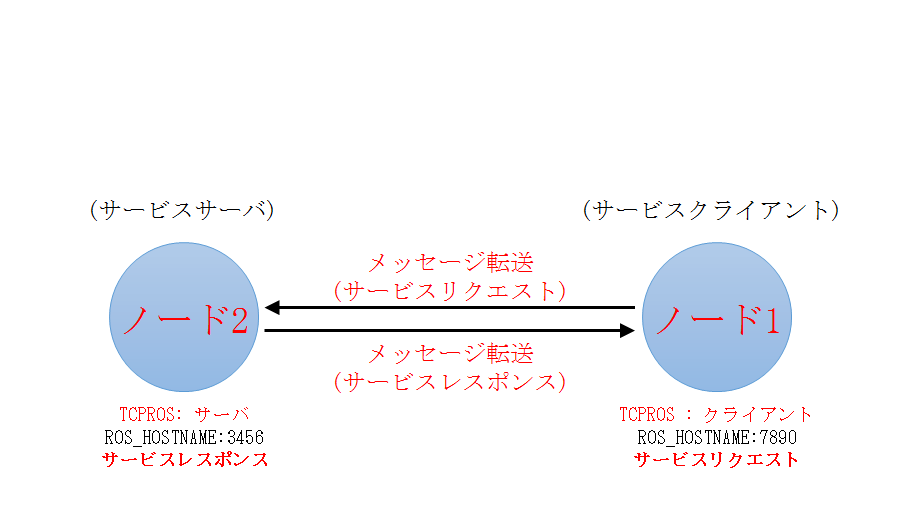
\includegraphics[width=12cm]{pictures/chapter3/pic_03_12.png}
  \caption{サービスメッセージ通信}
\end{figure}

%-------------------------------------------------------------------------------
\subsection{メッセージ通信の例}
2章では、turtlesimを利用して、ROSの動作をテストした。この例でもマスターと2つのノードが使用され、両方のノードが「/turtle1/cmd\_vel」というトピックを利用してメッセージ通信を行った。上記のROSにおける通信の手順に照らし合わせると、これは図3-13のように理解できる。

\begin{figure}[h]
  \centering
  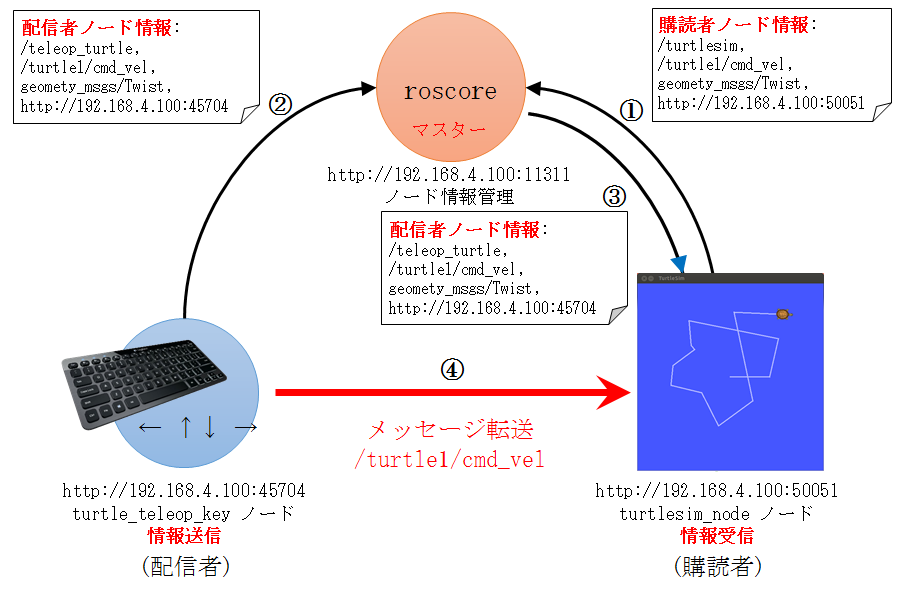
\includegraphics[width=12cm]{pictures/chapter3/pic_03_13.png}
  \caption{turtlesim におけるメッセージ通信の例}
\end{figure}

%-------------------------------------------------------------------------------
\section{ROSファイルシステム}
\index{ファイルシステム}\index{Filesystem}

OSのファイルシステムは、ROSのインストールフォルダとユーザー作業フォルダに分けられる。
ROSのデスクトップバージョンをインストールすると、/optフォルダにrosという名前でインストールフォルダが作成され、その中にroscoreを含む重要なユーティリティとrqt、RViz、ロボット関連のライブラリ、シミュレーション、ナビゲーションなどが置かれる。ユーザーが/optフォルダのファイルを触れることはほとんどない。もしバイナリファイルとして公式配布されているパッケージを変更しようとする場合は、「sudo apt-get install ros-indigo-xxx」などのパッケージのインストールコマンドではなく、直接、元のソースがあるリポジトリアドレスを確認し、「cd ~/catkin\_ws/src」 として作業フォルダ内のソースフォルダに移動し、「git clone [リポジトリアドレス]」のようにソースをコピーしてビルドすればよい。
ユーザー作業フォルダは、ユーザーが指定した任意の場所に作成できるが、特に問題がなければ、Linuxのユーザーフォルダに「~/catkin\_ws/」(「~/」は、Linux上で「/home/ユーザー名」に対応するフォルダ)を作成して利用する。
続いて、ROSのインストールフォルダとユーザー作業フォルダについて、さらに詳しく説明する。

%-------------------------------------------------------------------------------
\subsection{ROSのインストールフォルダ}
\index{インストール}\index{Install}

ROSは、「/opt/ros/[バージョン名]」フォルダにインストールされている。例えば、Indigoバージョンをインストールした場合、ROSがインストールされたフォルダは、次のとおりである。

\begin{itemize}
\item ROSのインストールフォルダ: /opt/ros/indigo
\end{itemize}

ROSのインストールフォルダである「/opt/ros/indigo」フォルダは、図3-14のように、「bin」、「etc」、「include」、「lib」、「share」などのフォルダと、環境設定ファイルで構成されている。

\begin{figure}[h]
  \centering
  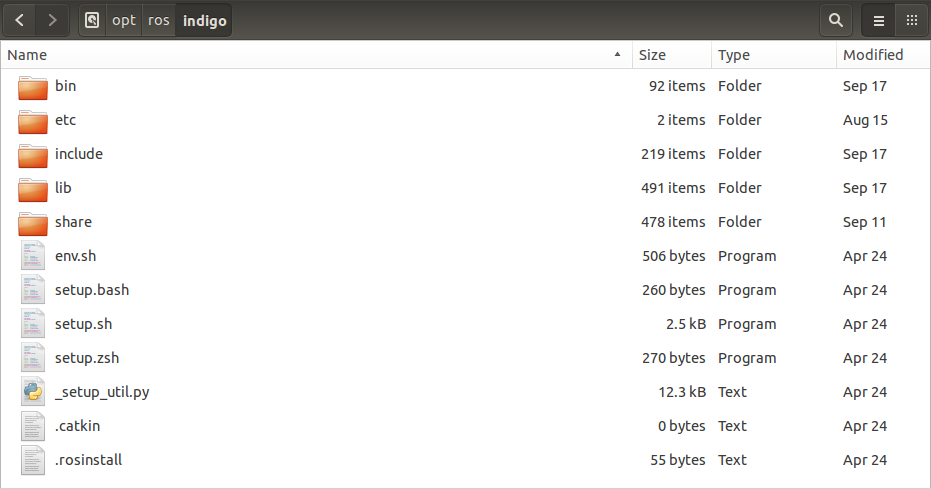
\includegraphics[width=12cm]{pictures/chapter3/pic_03_14.png}
  \caption{ROSファイルの構成}
\end{figure}

各フォルダの詳細は、次のとおりである。

\begin{itemize}
\item /bin    実行可能なバイナリファイル
\item /etc    ROSとcatkin関連の設定ファイル
\item /include  ヘッダーファイル
\item /lib    ライブラリファイル
\item /share  ROSパッケージ
\item env.*   環境設定ファイル
\item setup.* 環境設定ファイル
\end{itemize}

%-------------------------------------------------------------------------------
\subsection{ユーザー作業フォルダ}
\index{ユーザー作業フォルダ}

ユーザー作業フォルダは、ユーザーが指定した任意の場所に作成することができるが、本書では、ユーザー作業フォルダとして「~/catkin\_ws/」、あるいは「/home/ユーザー名/catkin\_ws」を使用する。例えば、ユーザー名が「irvs」でcatkinフォルダ名を「catkin\_ws」とすると、ユーザー作業フォルダは以下のフォルダとなる。

\begin{itemize}
\item ユーザー作業フォルダ: /home/irvs/catkin\_ws/
\end{itemize}

ユーザー作業フォルダは、ユーザーが作成したパッケージや、他の開発者が作成し、公開しているパッケージを保存し、ビルドする場所である。ユーザーは、ROSに関連するほとんどの作業を、このフォルダ内で行う。

%-------------------------------------------------------------------------------
\subsubsection{ファイルの構成}
ユーザー作業フォルダは、図3-15のようにbuild、devel、srcの3つのフォルダで構成されている。

\begin{figure}[h]
  \centering
  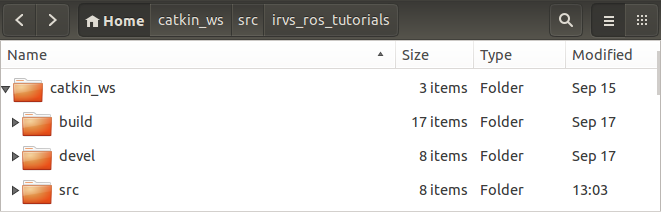
\includegraphics[width=12cm]{pictures/chapter3/pic_03_15.png}
  \caption{catkin workspaceのファイル構成}
\end{figure}

それぞれのフォルダの詳細は、次のとおりである。

\begin{itemize}
\item /build  ビルド関連ファイル
\item /devel  msg又はsrvのヘッダーファイルとユーザーパッケージのライブラリ、実行ファイル
\item /src    ユーザーパッケージ
\end{itemize}

%-------------------------------------------------------------------------------
\subsubsection{ユーザーパッケージ}
\index{Package}

「src」フォルダは、ユーザーのソースコードを置くフォルダである。このフォルダにユーザーが開発したROSパッケージや他のユーザーが開発したパッケージを保存する。図3-16は、著者が作成したirvs\_ros\_tutorialsというパッケージを展開した後の状態である。

\begin{figure}[h]
  \centering
  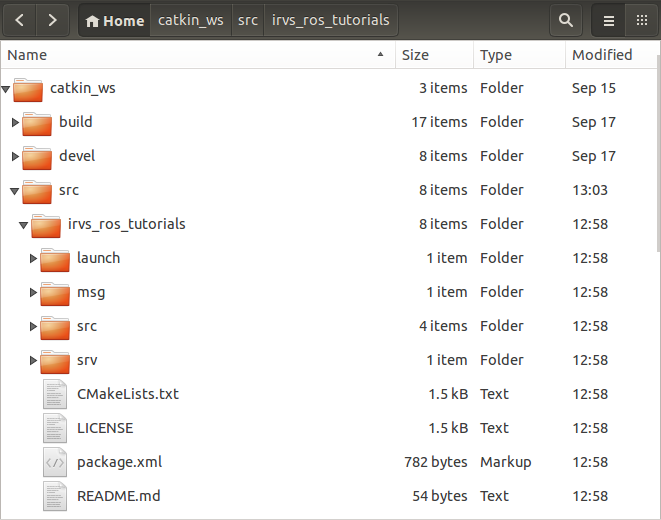
\includegraphics[width=12cm]{pictures/chapter3/pic_03_16.png}
  \caption{ユーザーパッケージのファイル構成}
\end{figure}

\begin{itemize}
\item /include    ヘッダーファイル
\item /launch   roslaunchに使用されるlaunchファイル
\item /node     rospy用スクリプト
\item /msg      メッセージのファイル
\item /src      ソースコードファイル
\item /srv      サービスファイル
\item CMakeLists.txt  ビルドの設定ファイル
\item package.xml   パッケージの設定ファイル
\end{itemize}

%-------------------------------------------------------------------------------
\section{ROSビルドシステム}
\index{ビルドシステム}\index{Build System}

ROSのビルドシステムは、ROSパッケージをマルチプラットフォームで開発するため、基本的にはCMake(Cross Platform Make)\footnote{\url{https://ja.wikipedia.org/wiki/CMake}}を利用している。catkinビルドシステムは、CMakeをROSに合わせて改良したものであり、CMakeと同様にパッケージのフォルダ内のCMakeLists.txtファイルにビルド環境を記述している。Make\footnote{\url{https://ja.wikipedia.org/wiki/Make}}がUnix系を主な対象としているのとは異なり、CMakeは、Unix系のLinux、BSD、Mac OS Xだけでなく、Windows系にも対応している。また、マイクロソフトのVisual Studioもサポートしており、Qt\footnote{\url{http://www.qt.io/}}の開発にも容易に適用できる。さらに、catkinビルドシステムは、ROSに関連するビルド、パッケージ管理、依存関係パッケージの自動インストールなども容易に実行できる。

%-------------------------------------------------------------------------------
\subsection{パッケージの作成}
\index{Package}

ROSパッケージを作成するコマンドは次のとおりである。

\begin{lstlisting}[language=ROS]
$ catkin_create_pkg %*[パッケージ名] [依存するパッケージ1]…[依存するパッケージn]*)
\end{lstlisting}

「catkin\_create\_pkg」コマンドを実行すると、catkinビルドシステムに必要なCMakeLi\\sts.txtとpackage.xmlを含む空のパッケージフォルダが作成される。実際に簡単なパッケージを作成してみよう。まず、次のコマンドでユーザー作業フォルダの「src」フォルダに移動する。

\begin{lstlisting}[language=ROS]
$ cd ~/catkin_ws/src
\end{lstlisting}

ここで作成するパッケージの名前は「my\_first\_ros\_pkg」である。 ROSのパッケージ名には、通常はすべて小文字を使用し、スペースは使用できない。またハイフン(-)ではなくアンダースコア(\_)を使用し、各単語を続ける。ROSプログラミングにおけるコーディングスタイルと名前の規則については、関連ページ\footnote{\url{http://wiki.ros.org/StyleGuide}}\footnote{\url{http://wiki.ros.org/CppStyleGuide}}\footnote{\url{http://wiki.ros.org/Names}}を参照してほしい。
では、次のコマンドでmy\_first\_ros\_pkgという名前のパッケージを作成しよう。

\begin{lstlisting}[language=ROS]
$ catkin_create_pkg my_first_ros_pkg std_msgs roscpp
\end{lstlisting}

上記のコマンドでは、依存するパッケージ「std\_msgs」と「roscpp」をオプションとして記述している。これは作成するパッケージでは、ROSの標準的なメッセージパッケージstd\_msgsとC/C++を使用するためのクライアントライブラリroscppを使用するため、パッケージの作成に先立ってこれらをインストールしておく必要があることを意味する。依存するパッケージの設定は、上記のようにパッケージの作成時に指定する方法もあるが、生成されたフォルダ内の「package.xml」に後から直接記述してもよい。
パッケージを作成すると、「~/catkin\_ws/src」の下に「my\_first\_ros\_pkg」というパッケージのフォルダが作成され、その中にROSパッケージが備えるべき基本的なフォルダと、CMakeLists.txtとpackage.xmlファイルが生成される。次のように「ls」コマンドや、UbuntuのGUIベースのNautilusを利用して、パッケージの内部を見てみよう。

\begin{lstlisting}[language=ROS]
$ ls
include
src
CMakeLists.txt
package.xml
\end{lstlisting}

\begin{figure}[h]
  \centering
  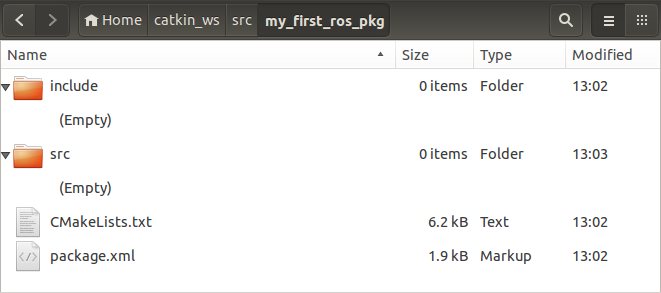
\includegraphics[width=12cm]{pictures/chapter3/pic_03_17.png}
  \caption{自動生成されたファイルとフォルダ}
\end{figure}

 %-------------------------------------------------------------------------------
 \subsection{パッケージ設定ファイル(package.xml)の変更}
 \index{package.xml}

ROSのパッケージの設定ファイルであるpackage.xmlは、パッケージの名前、著作者、ライセンス、依存性パッケージなどのパッケージの情報を、XMLファイルとして保存している。作成直後のpackage.xmlファイルは、以下の通りである。

ファイル名:package.xml

\begin{lstlisting}[language=ROS]
<?xml version="1.0"?>
<package>
<name>my_first_ros_pkg</name>
<version>0.0.0</version>
<description>The my_first_ros_pkg package</description>

<!-- One maintainer tag required, multiple allowed, one person per tag -->
<!-- Example:  -->

<!-- <maintainer email="jane.doe@example.com">Jane Doe</maintainer> -->
<maintainer email="rt@todo.todo">rt</maintainer>

<!-- One license tag required, multiple allowed, one license per tag -->
<!-- Commonly used license strings: -->
<!-- BSD, MIT, Boost Software License, GPLv2, GPLv3, LGPLv2.1, LGPLv3 -->
<license>TODO</license>

<!-- Url tags are optional, but mutiple are allowed, one per tag -->
<!-- Optional attribute type can be: website, bugtracker, or repository -->
<!-- Example: -->
<!-- <url type="website">http://wiki.ros.org/my_first_ros_pkg</url> -->

<!-- Author tags are optional, mutiple are allowed, one per tag -->
<!-- Authors do not have to be maintianers, but could be -->
<!-- Example: -->
<!-- <author email="jane.doe@example.com">Jane Doe</author> -->

<!-- The *_depend tags are used to specify dependencies -->
<!-- Dependencies can be catkin packages or system dependencies -->
<!-- Examples: -->
<!-- Use build_depend for packages you need at compile time: -->
<!-- <build_depend>message_generation</build_depend> -->
<!-- Use buildtool_depend for build tool packages: -->
<!-- <buildtool_depend>catkin</buildtool_depend> -->
<!-- Use run_depend for packages you need at runtime: -->
<!-- <run_depend>message_runtime</run_depend> -->
<!-- Use test_depend for packages you need only for testing: -->
<!-- <test_depend>gtest</test_depend> -->
<buildtool_depend>catkin</buildtool_depend>
<build_depend>roscpp</build_depend>
<build_depend>std_msgs</build_depend>
<run_depend>roscpp</run_depend>
<run_depend>std_msgs</run_depend>

<!-- The export tag contains other, unspecified, tags -->
<export>
<!-- You can specify that this package is a metapackage here: -->
<!-- <metapackage/> -->
<!-- Other tools can request additional information be placed here -->
</export>
</package>
\end{lstlisting}

各構文について説明する。

\begin{itemize}
\item <? xml> ドキュメントの文法を定義する構文で、以下の内容は、xmlバージョン1.0であることを意味する。
\item <package> この構文から</package>までがROSパッケージの設定部分である。
\item <name> パッケージの名前である。パッケージを作成するときに入力したパッケージ名が使用される。他のオプションも同じであるが、パッケージ名はユーザーが必要なときにいつでも変更することができる。ただし、後で説明するCMakeLists.txtファイルの「project」部分と一致していなければならない。
\item <version> パッケージのバージョンである。自由に指定することができる。
\item <description> パッケージの簡単な説明である。
\item <maintainer> パッケージマネージャの連絡先を記載する。
\item <license> ライセンスを記載する。 BSD、MIT、GPLv3、LGPLv3などを記載すればよい。
\item <url> パッケージを説明しているWebページまたはバグ管理、ストレージなどのアドレスを記載する。種類に応じてtypeにはwebsite、bugtracker、repositoryを記載すればよい。
\item <author> パッケージの開発に参加した開発者を示す。複数の開発者が参加した場合は、次の行に<author>タグを使用して、追加すれば良い。
\item <buildtool\_depend> ビルドシステムの依存関係を記述する。現在はcatkinビルドシステムを利用しているのでcatkinと記述する。
\item <build\_depend> パッケージをビルドするときに依存するパッケージの名前を書く。
\item <run\_depend> パッケージを実行するときに依存するパッケージの名前を書く。
\item <test\_depend> パッケージをテストするときに依存するパッケージの名前を書く。
\item <export> ROSで明示していないタグ名を使用するときに使われる。ただし、使用頻度は低い。
\item <metapackage> exportタグ内で使用するタグであり、現在のパッケージがメタパッケージであれば、ここで宣言する。
\end{itemize}

上述した作成直後のファイルに必要な情報を追加し、不要な行を削除したパッケージ設定ファイル(package.xml)の一例を示す。

ファイル名:package.xml

\begin{lstlisting}[language=XML]
<?xml version="1.0"?>
<package>
<name>my_first_ros_pkg</name>
<version>0.0.1</version>
<description>The my_first_ros_pkg package</description>

<maintainer email = "aaa@bbb.jp">Anonymous</maintainer>

<license>BSD</license>
<url type = "website"> http://irvs.github.io/ros_tms/</url>
<url type="repository">https://github.com/irvs/irvs_ros_tutorials.git</url>
<author email = "aaa@bbb.jp">Anonymous</author>

<buildtool_depend>catkin</buildtool_depend>

<build_depend>std_msgs</build_depend>
<build_depend>roscpp</build_depend>

<run_depend>std_msgs</run_depend>
<run_depend>roscpp</run_depend>

<export>
</export>
</package>
\end{lstlisting}

%-------------------------------------------------------------------------------
\subsection{ビルド設定ファイル(CMakeLists.txt)の変更}
\index{CMakeLists.txt}

ROSのビルドシステムであるcatkinでは、パッケージのフォルダ内のCMakeLists.txtファイルにビルドの環境を記述している。このCMakeLists.txtファイルには、作成するパッケージ名、依存パッケージ名、実行可能ファイル名などを設定する。作成直後のCMakeLists.txtファイルは、以下の通りである。

ファイル名:CMakeLists.txt

\begin{lstlisting}[language=make]
cmake_minimum_required(VERSION 2.8.3)
project(my_first_ros_pkg)

## Find catkin macros and libraries
## if COMPONENTS list like find_package(catkin REQUIRED COMPONENTS xyz)
## is used, also find other catkin packages
find_package(catkin REQUIRED COMPONENTS roscpp std_msgs)

## System dependencies are found with CMake's conventions
# find_package(Boost REQUIRED COMPONENTS system)

## Uncomment this if the package has a setup.py. This macro ensures
## modules and global scripts declared therein get installed
## See http://ros.org/doc/api/catkin/html/user_guide/setup_dot_py.html
# catkin_python_setup()

################################################
## Declare ROS messages, services and actions ##
################################################

## To declare and build messages, services or actions from within this
## package, follow these steps:
## * Let MSG_DEP_SET be the set of packages whose message types you use in
##  your messages/services/actions (e.g. std_msgs, actionlib_msgs, ...).
## * In the file package.xml:
##  * add a build_depend and a run_depend tag for each package in MSG_DEP_SET
##  * If MSG_DEP_SET isn't empty the following dependencies might have been
##  pulled in transitively but can be declared for certainty nonetheless:
##  * add a build_depend tag for "message_generation"
##  * add a run_depend tag for "message_runtime"
## * In this file (CMakeLists.txt):
##  * add "message_generation" and every package in MSG_DEP_SET to
##  find_package(catkin REQUIRED COMPONENTS ...)
##  * add "message_runtime" and every package in MSG_DEP_SET to
##  catkin_package(CATKIN_DEPENDS ...)
##  * uncomment the add_*_files sections below as needed
##  and list every .msg/.srv/.action file to be processed
##  * uncomment the generate_messages entry below
##  * add every package in MSG_DEP_SET to generate_messages(DEPENDENCIES ...)

## Generate messages in the 'msg' folder
# add_message_files(
# FILES
# Message1.msg
# Message2.msg
# )

## Generate services in the 'srv' folder
# add_service_files(
# FILES
# Service1.srv
# Service2.srv
# )

## Generate actions in the 'action' folder
# add_action_files(
# FILES
# Action1.action
# Action2.action
# )

## Generate added messages and services with any dependencies listed here
# generate_messages(
# DEPENDENCIES
# std_msgs
# )

###################################
## catkin specific configuration ##
###################################
## The catkin_package macro generates cmake config files for your package
## Declare things to be passed to dependent projects
## INCLUDE_DIRS: uncomment this if you package contains header files
## LIBRARIES: libraries you create in this project that dependent projects also need
## CATKIN_DEPENDS: catkin_packages dependent projects also need
## DEPENDS: system dependencies of this project that dependent projects also need catkin_package(
#  INCLUDE_DIRS include
#  LIBRARIES my_first_ros_pkg
#  CATKIN_DEPENDS roscpp std_msgs
#  DEPENDS system_lib
)

###########
## Build ##
###########

## Specify additional locations of header files
## Your package locations should be listed before other locations
# include_directories(include) include_directories(
${catkin_INCLUDE_DIRS}
)

## Declare a cpp library
# add_library(my_first_ros_pkg
# src/${PROJECT_NAME}/my_first_ros_pkg.cpp
# )

## Declare a cpp executable
# add_executable(my_first_ros_pkg_node src/my_first_ros_pkg_node.cpp)

## Add cmake target dependencies of the executable/library
## as an example, message headers may need to be generated before nodes
# add_dependencies(my_first_ros_pkg_node my_first_ros_pkg_generate_messages_cpp)

## Specify libraries to link a library or executable target against
# target_link_libraries(my_first_ros_pkg_node
# ${catkin_LIBRARIES}
# )

#############
## Install ##
#############

# all install targets should use catkin DESTINATION variables
# See http://ros.org/doc/api/catkin/html/adv_user_guide/variables.html

## Mark executable scripts (Python etc.) for installation
## in contrast to setup.py, you can choose the destination
# install(PROGRAMS
# scripts/my_python_script
# DESTINATION ${CATKIN_PACKAGE_BIN_DESTINATION}
# )

## Mark executables and/or libraries for installation
# install(TARGETS my_first_ros_pkg my_first_ros_pkg_node
# ARCHIVE DESTINATION ${CATKIN_PACKAGE_LIB_DESTINATION}
# LIBRARY DESTINATION ${CATKIN_PACKAGE_LIB_DESTINATION}
# RUNTIME DESTINATION ${CATKIN_PACKAGE_BIN_DESTINATION}
# )

## Mark cpp header files for installation
# install(DIRECTORY include/${PROJECT_NAME}/
# DESTINATION ${CATKIN_PACKAGE_INCLUDE_DESTINATION}
# FILES_MATCHING PATTERN "*.h"
# PATTERN ".svn" EXCLUDE
# )

## Mark other files for installation (e.g. launch and bag files, etc.)
# install(FILES
# # myfile1
# # myfile2
# DESTINATION ${CATKIN_PACKAGE_SHARE_DESTINATION}
# )

#############
## Testing ##
#############

## Add gtest based cpp test target and link libraries
# catkin_add_gtest(${PROJECT_NAME}-test test/test_my_first_ros_pkg.cpp)
# if(TARGET ${PROJECT_NAME}-test)
# target_link_libraries(${PROJECT_NAME}-test ${PROJECT_NAME})
# endif()

## Add folders to be run by python nosetests
# catkin_add_nosetests(test)
\end{lstlisting}

ビルド設定ファイル(CMakeLists.txt)の各オプションは、次の通りである。

\begin{lstlisting}[language=make]
cmake_minimum_required(VERSION 2.8.3)
\end{lstlisting}

オペレーティングシステムにインストールされているcmakeの最低限必要なバージョンである。この例では2.8.3バージョンと記載されているので、これ以前のバージョンのcmakeを利用している場合は、cmakeを更新する必要がある。

\begin{lstlisting}[language=make]
project(my_first_ros_pkg)
\end{lstlisting}

パッケージの名前である。「package.xml」で入力したパッケージ名をそのまま使用する。もしpackage.xmlの<name>タグに記述したパッケージ名と異なる場合は、ビルドするときにエラーが発生する。

\begin{lstlisting}[language=make]
find_package(catkin REQUIRED COMPONENTS roscpp std_msgs)
\end{lstlisting}

catkinビルドをするときに必要なコンポーネントパッケージ、すなわち依存パッケージを指定する。この例では、依存パッケージとしてroscppとstd\_msgsが指定されている。ここで指定されたパッケージが存在しない場合、ビルドするときにエラーが表示される。

\begin{lstlisting}[language=make]
find_package(Boost REQUIRED COMPONENTS system)
\end{lstlisting}

ROS以外のパッケージまたはライブラリを使用するときの記述方法である。この例では、BoostというC++ライブラリを使用する際、systemというBoostのコンポーネントライブラリがインストールされていなければならないことを意味する。

\begin{lstlisting}[language=make]
catkin_python_setup()
\end{lstlisting}

Pythonを使用する時に設定するオプションである。Pythonのインストールプロセスであるsetup.py\footnote{\url{https://docs.python.org/2/distutils/setupscript.html}}を呼ぶ。

\begin{lstlisting}[language=make]
add_message_files (FILES
  Message1.msg
  Message2.msg
)
\end{lstlisting}

使用するメッセージファイルを追加するためのオプションである。FILESの後に使用するメッセージファイル(*.msg)を記述しておくと、現在のパッケージフォルダのmsgフォルダ内のmsgファイルを参照し、関連するヘッダーファイルを自動生成する。この例では、Message1.msgとMessage2.msgのメッセージファイルを利用する。

\begin{lstlisting}[language=make]
add_service_files (FILES
  Service1.srv
  Service2.srv
)
\end{lstlisting}

使用するサービスファイルを追加するためのオプションである。 FILESの後に使用するサービスファイル(*.srv)を記述しておくと、現在のパッケージフォルダのsrvフォルダ内のsrvファイルを参照し、関連するヘッダーファイルを自動生成する。この例では、Service1.srvとService2.srvのサービスファイルを利用する。

\begin{lstlisting}[language=make]
generate_messages (DEPENDENCIES std_msgs)
\end{lstlisting}

依存しているメッセージを設定するためのオプションである。この例では、DEPENDENCIESオプションによってstd\_msgsというメッセージパッケージを使用する。

\begin{lstlisting}[language=make]
catkin_package (INCLUDE_DIRS include
     LIBRARIES my_first_ros_pkg
     CATKIN_DEPENDS roscpp std_msgs
     DEPENDS system_lib
)
\end{lstlisting}

catkinビルドオプションである。 INCLUDE\_DIRSではヘッダーファイルの置かれたフォルダを指定し、ここではパッケージフォルダのincludeフォルダを指定している。LIBRARIESでは、「add\_library」で指定したライブラリの保存先フォルダを指定する。このLIBRARIES フォルダは「catkin\_ws/devel/lib」の下に生成される。CATKIN\_DEPENDSはroscppやstd\_msgなど、依存するパッケージを指定し、上の例ではroscppとstd\_msgsが依存していると設定している。DEPENDSはシステム依存のパッケージを記述するための設定である。

\begin{lstlisting}[language=make]
include_directories (${catkin_INCLUDE_DIRS})
\end{lstlisting}

インクルードフォルダを指定できるオプションである。この例では、\${catkin\_INCLU\\DE\_DIRS}と設定されているが、これは生成したパッケージ内のincludeフォルダを意味し、この中のヘッダーファイルを利用する。

\begin{lstlisting}[language=make]
add_library (my_first_ros_pkg src/${PROJECT_NAME}/my_first_ros_pkg.cpp)
\end{lstlisting}

ビルドする際、作成するライブラリを指定する。この例では、src/\${PROJECT\_NAME} /my\_first\_ros\_pkg.cppファイルを参照して、my\_first\_ros\_pkgというライブラリを作成する。

\begin{lstlisting}[language=make]
add_executable (my_first_ros_pkg_node src/my_first_ros_pkg_node.cpp)
\end{lstlisting}

ビルドする際、作成する実行可能ファイルを指定する。この例では、src/my\_first\_ros\\\_pkg\_node.cppファイルを参照して、my\_first\_ros\_pkg\_nodeという実行ファイルを生成する。

\begin{lstlisting}[language=make]
add_dependencies (my_first_ros_pkg_node my_first_ros_pkg_generate_messages_cpp)
\end{lstlisting}

パッケージをビルドする前に、メッセージのヘッダーファイルを作成する必要がある場合、パッケージのビルド前にメッセージファイルを生成するための設定である。この例では、my\_first\_ros\_pkg\_generate\_messages\_cppとしてmsgやsrv関連ヘッダーファイルを優先的に生成した後で、my\_first\_ros\_pkg\_nodeをビルドする。

\begin{lstlisting}[language=make]
target_link_libraries (my_first_ros_pkg_node
${catkin_LIBRARIES}
)
\end{lstlisting}

my\_first\_ros\_pkg\_nodeを作成する際に、リンクするライブラリを指定するオプションである。
作成直後のファイルから不要な行を削除したビルド設定ファイル(CMakeLists.txt)を示す。

ファイル名:CMakeLists.txt
\begin{lstlisting}[language=make]
cmake_minimum_required(VERSION 2.8.3)
project(my_first_ros_pkg)

find_package(catkin REQUIRED COMPONENTS roscpp std_msgs)

catkin_package( INCLUDE_DIRS include
    CATKIN_DEPENDS roscpp std_msgs
    DEPENDS system_lib
)

include_directories( ${catkin_INCLUDE_DIRS} )

add_executable(hello_world_node src/hello_world_node.cpp) add_dependencies(hello_world_node my_first_ros_pkg_generate_messages_cpp) target_link_libraries(hello_world_node ${catkin_LIBRARIES})
\end{lstlisting}

%-------------------------------------------------------------------------------
\subsection{ソースコードの作成}
上述したCMakelists.txtファイルにおいて、実行ファイルを作成する部分(add\_executab\\le)には次のように記述した。

\begin{lstlisting}[language=ROS]
add_executable (hello_world_node src/hello_world_node.cpp)
\end{lstlisting}

これは、パッケージフォルダのsrcフォルダ内にあるhello\_world\_node.cppソースコードから、hello\_world\_nodeという名前の実行ファイルを生成する設定である。しかし、まだhello\_world\_node.cppというファイルがないので、作成してみよう。
まず、「cd」コマンドで作成したパッケージフォルダ内のソースコードを保存するフォルダ(src)に移動し、hello\_world\_node.cppファイルを生成する。次の例では、geditというエディタを使用したが、sublime text、vim、emacs、nanoなど好きなエディタを利用してかまわない。

\begin{lstlisting}[language=ROS]
$ cd ~/catkin_ws/src/my_first_ros_pkg/src
$ gedit hello_world_node.cpp
\end{lstlisting}

次に、以下のソースコードを作成し、保存する。

ファイル名:hello\_world\_node.cpp

\begin{lstlisting}[language=C++]
#include <ros/ros.h>
#include <std_msgs/String.h>
#include <sstream>

int main(int argc, char **argv)
{
  ros::init(argc, argv, "hello_world_node");
  ros::NodeHandle nh;
  ros::Publisher chatter_pub =
    nh.advertise<std_msgs::String>("say_hello_world", 1000);
  ros::Rate loop_rate(10);
  int count = 0;
  while (ros::ok())
  {
    std_msgs::String msg;
    std::stringstream ss;
    ss << "hello world " << count;
    msg.data = ss.str();
    ROS_INFO("%s", msg.data.c_str());
    chatter_pub.publish(msg);
    ros::spinOnce();
    loop_rate.sleep();
    ++count;
  }
  return 0;
}
\end{lstlisting}

%-------------------------------------------------------------------------------
\subsection{パッケージのビルド}
\index{ビルドシステム}\index{Build System}\index{catkin\_make}

これで、パッケージをビルドするためのすべての準備作業が終了した。次はユーザー作業フォルダに移動し、catkinビルドを実行しよう。

\begin{lstlisting}[language=ROS]
$ cd ~/catkin_ws && catkin_make
\end{lstlisting}

\begin{exercise}[短縮コマンド]
先に2.2節「ROSの開発環境の構築」で述べたように、「.bash\\rc」ファイルに「alias cm='cd ~/catkin\_ws \&\& catkin\_make'」と設定しておくと、ターミナルウィンドウで「cm」と入力するだけで、上のコマンドを実行できる。
\end{exercise}

%-------------------------------------------------------------------------------
\subsection{ノードの実行}
\index{ノード}\index{Node}

これで、パッケージをビルドするためのすべての準備作業が終了した。次はユーザー作業フォルダに移動し、catkinビルドを実行しよう。

エラーがなくビルドが終了したら、「~/catkin\_ws/devel/lib/my\_first\_ros\_pkg」に「hello\_\\world\_node」という名前のファイルが生成されている。次のステップは、ノードの実行である。ただし、ROSのすべてのノードは、roscoreを実行して初めて利用できるので、必ず先にroscoreを実行しておく必要がある。

\begin{lstlisting}[language=ROS]
$ roscore
\end{lstlisting}

最後に、新しいターミナルウィンドウを開き、次のコマンドでノードを実行してみよう。これは、my\_first\_ros\_pkgという名前のパッケージのhello\_world\_nodeという名前のノードを実行するコマンドである。

\begin{lstlisting}[language=ROS]
$ rosrun my_first_ros_pkg hello_world_node
[INFO] [1423443540.131775283]: hello world 0
[INFO] [1423443540.231826916]: hello world 1
[INFO] [1423443540.331798085]: hello world 2
[INFO] [1423443540.431796634]: hello world 3
[INFO] [1423443540.531808660]: hello world 4
[INFO] [1423443540.631800431]: hello world 5
[INFO] [1423443540.731805683]: hello world 6
\end{lstlisting}

ノードを実行すると、hello world 0、1、2などのメッセージが配信されていることが確認できる。

%-------------------------------------------------------------------------------

% !TEX root = ./rosbook_jp.tex
%-------------------------------------------------------------------------------
\chapterimage{chapter_head_4.pdf}

%-------------------------------------------------------------------------------
\chapter{ROS コマンド}\index{ROS コマンド}

ROSは、Ubuntuのコマンドラインインタフェース (CLI)であるシェル(shell)環境で、様々なコマンドを使用して、ファイルシステムの利用、ソースコードの編集、ビルド、デバッグ、パッケージ管理などを行う。ROSを利用するには、基本的なLinuxコマンドに加えて、ROS固有のコマンド注1を修得する必要がある。本章では、それらのROS固有のコマンドを、ROSシェルコマンド、ROS実行コマンド、ROS情報コマンド、ROS catkinコマンド、ROSパッケージのコマンドに分けて説明する。主な用途を以下に示す。

\begin{itemize}
\item ROSシェルコマンド: コピーなどのファイル操作やディレクトリ操作
\item ROS実行コマンド: ノードの実行
\item ROS情報コマンド: ノードやメッセージ情報の表示
\item ROS catkinコマンド: パッケージのビルド
\item ROSパッケージのコマンド: パッケージのインストールや依存関係の表示
\end{itemize}

なお、コマンドの後のアスタリスクは、そのコマンドの使用頻度を表している。

%-------------------------------------------------------------------------------
\section{ROSシェルコマンド}\index{ROSシェルコマンド}

ROSシェルコマンドはrosbashと呼ばれ、Linuxで一般的に使用されるbashシェルコマンドに類似した、ROS特有のシェルコマンドである。

\vspace{\baselineskip}
\noindent
\begin{description}
\item[roscd](★★★)ros+cd(changes directory):指定されたROSパッケージのディレクトリに移動
\item[rosls] (★☆☆)ros+ls(lists files):ROSパッケージのファイルリストを確認
\item[rosed](★☆☆)ros+ed(editor):ROSパッケージのファイルを編集
\item[roscp] (★☆☆)ros+cp(copies files):ROSパッケージのファイルをコピー
\item[rospd](☆☆☆)ros+pushd:ROSディレクトリインデックスにディレクトリを追加
\item[rosd](☆☆☆)ros+directory:ROSディレクトリインデックスを確認
\end{description}

このうち、頻繁に使用されるroscd、rosls、rosedコマンドについて詳しく述べる。

\begin{exercise}[ROSシェルコマンドを使用できる環境]
    ROSシェルコマンドは、次のコマンドでrosbashがインストールされており、「source /opt/ros/<ros distribution>/setup.bash」が設定された端末で使用できる。2章のROSのインストールが正しく行われていれば、すぐに使用できる。
  \begin{lstlisting}[language=ROS]
  $ sudo apt-get install ros-<ros distribution>-rosbash
  \end{lstlisting}
  例えば、ROSのバージョンがindigoであれば以下のコマンドである。
  \begin{lstlisting}[language=ROS]
  $ sudo apt-get install ros-indigo-rosbash
  $ source /opt/ros/indigo/setup.bash
  \end{lstlisting}
\end{exercise}

%-------------------------------------------------------------------------------
\subsection{roscd:ROSパッケージのディレクトリへ移動}

roscdは、パッケージの保存先のディレクトリに移動するコマンドである。自分が作成したパッケージやインストールしたパッケージの名前を、パラメータとしてこのコマンドに続けて入力すると、そのパッケージの置かれたディレクトリに移動する。使用頻度は非常に高い。

\begin{itemize}
\item roscd [パッケージ名]
\end{itemize}

下の例は、ROSのインストールフォルダにあるturtlesimパッケージに移動している様子である。

\begin{lstlisting}[language=ROS]
$ roscd turtlesim
/opt/ros/indigo/share/turtlesim$
\end{lstlisting}

なお、上の例では、関連するパッケージであるros-indigo-turtlesimがインストールされている必要がある。インストールされていない場合は、次のコマンドでインストールできる。

\begin{lstlisting}[language=ROS]
$ sudo apt-get install ros-indigo-turtlesim
\end{lstlisting}

%-------------------------------------------------------------------------------
\subsection{rosls:ROSファイルのリスト表示}

roslsは指定されたROSパッケージ内のファイルの一覧を表示するコマンドである。パッケージ名をこのコマンドに続けて入力すると、そのパッケージを検索し、パッケージ内のファイルの一覧を表示する。

\begin{itemize}
\item  rosls [パッケージ名]
\end{itemize}

\begin{lstlisting}[language=ROS]
$ rosls turtlesim
cmake images msg package.xml srv
\end{lstlisting}

%-------------------------------------------------------------------------------
\subsection{rosed:ROSファイルの編集}

rosedはパッケージ内のファイルを編集するときに使用するコマンドであり、ユーザーが設定したエディタでファイルを開く。比較的簡単な内容を手軽に修正するときに使用する。この時、使用されるエディタは、「~/.bashrc」ファイルに「export EDITOR= 'nano'」のように指定する。

\begin{itemize}
\item   rosed [パッケージ名] [ファイル名]
\end{itemize}

\begin{lstlisting}[language=ROS]
$ rosed turtlesim package.xml
\end{lstlisting}

%-------------------------------------------------------------------------------
\section{ROS実行コマンド}\index{ROS実行コマンド}

ROS実行コマンドは、ROSノードの実行を制御する。特にroscoreはROSネームサーバであるROSマスター、標準出力・標準エラー出力のためのrosout、パラメータを管理するパラメータサーバを同時に起動するものであり、他のノードの実行前に実行する必要がある。ノードの実行コマンドには、rosrunとroslaunchがある。rosrunは単一のノードを実行するものであり、roslaunchは複数のノードを実行する。また、roscleanは、ノードの実行時に記録されるログを削除するコマンドである。

\vspace{\baselineskip}
\noindent
\begin{description}
\item[roscore](★★★)ros+core:ROSマスター(ROSネームサーバ)、rosout(標準出力stdout/標準エラー出力stderr)、パラメータサーバ(パラメータ管理)の起動
\item[rosrun](★★★)ros+run:パッケージの一つのノードを実行
\item[roslaunch](★★★)ros+launch:パッケージの複数のノードを同時実行
\item[rosclean](★★☆)ros+clean:rosログファイルを確認、削除
\end{description}

%-------------------------------------------------------------------------------
\subsection{roscore:ROSマスター、rosout、パラメータサーバの起動}

roscoreは、ノード間のメッセージ通信の接続情報を管理するROSマスターを起動するコマンドである。起動されたROSマスターはXMLRPCのサーバとなる。ROSマスターは、ROSの使用にあたって最初に起動しておく必要がある。roscoreを実行すると、ユーザーが設定した「~/.bashrc」中のROS\_MASTER\_URIをマスターURIとし、ROSマスターが立ち上がる。

\setcounter{num}{0}

\begin{lstlisting}[language=ROS]
$ roscore
... logging to /home/xxx/.ros/log/f4b17da6-ecda-11e4-a7bf-d43d7e970cb0/roslaunch-rt-18869.log \stepcounter{num}\circled{\thenum} )
Checking log directory for disk usage. This may take a while.
Press Ctrl-C to interrupt  \stepcounter{num}\circled{\thenum}
Done checking log file disk usage. Usage is <1GB.

started roslaunch server http://192.168.4.100:47915/
ros_comm version 1.11.10


SUMMARY
========

PARAMETERS
 * /rosdistro: indigo \stepcounter{num}\circled{\thenum}
 * /rosversion: 1.11.10 \stepcounter{num}\circled{\thenum}

NODES

auto-starting new master
process[master]: started with pid [18881]
ROS_MASTER_URI=http://192.168.4.100:11311/ \stepcounter{num}\circled{\thenum}

setting /run_id to f4b17da6-ecda-11e4-a7bf-d43d7e970cb0
process[rosout-1]: started with pid [18894]
started core service [/rosout] \stepcounter{num}\circled{\thenum}
\end{lstlisting}

上記の出力結果の太字部分から、①「/home/xxx/.ros/log/」フォルダにログが保存されていること、②<Ctrl>+<C>でroscoreを終了ができること、③「/rosdistro」と④「/rosversion」がパラメータとしてパラメータサーバに登録されたこと、⑤ROS\_MASTER\_URIの情報、⑥「/rosout」ノードが実行されたことなどが確認できる。

\begin{exercise}[ログの保存場所]
上の例ではlogが保存される場所が「/home/xxx/.ros/log/」(xxxはユーザー名)となっているが、ROS\_HOME環境変数を設定することで任意の場所に保存できる。変数が設定されていない場合は「/home/xxx/.ros/log/」に記録される。
\end{exercise}

%-------------------------------------------------------------------------------
\subsection{rosrun:ROSノードの実行}

rosrunは、指定したパッケージ内の1つのノードを実行するコマンドである。

\begin{itemize}
\item   rosrun [パッケージ名] [ノード名]
\end{itemize}

以下の例では、turtlesimパッケージ内のturtlesim\_nodeノードを実行する。実行結果を図4-1に示す。

\begin{lstlisting}[language=ROS]
$ rosrun turtlesim turtlesim_node
[INFO] [1430205691.820701916]: Starting turtlesim with node name /turtlesim
[INFO] [1430205691.827666004]: Spawning turtle [turtle1] at x=[5.544445], y=[5.544445], theta=[0.000000]
\end{lstlisting}

\begin{figure}[htp]
  \centering
  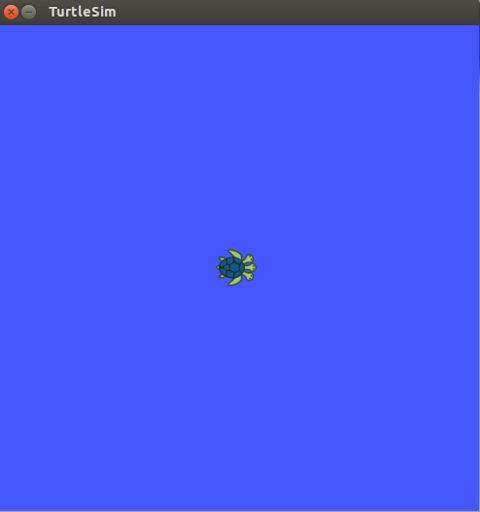
\includegraphics[width=\columnwidth]{pictures/chapter4/pic_04_01.png}
  \caption{turtlesim\_nodeノードを実行した様子}
\end{figure}


%-------------------------------------------------------------------------------
\subsection{roslaunch:複数のROSノードの実行}

roslaunchは、指定されたパッケージから1つ以上のノードを実行するコマンドである。

\begin{itemize}
\item   roslaunch [パッケージ名] [launchファイル名]
\end{itemize}

roslaunchは、複数のノードを実行する際に非常に有用であり、頻繁に使用されるノードの実行方法である。launchファイルの作成法については、6.5節「roslaunchの使い方」で詳細に取り上げる。
下の例のようにopenni\_launchパッケージ内のopenni.launchファイルを実行するだけで、camera\_nodelet\_manager、depth\_metric、depth\_metric\_rect、depth\_pointsなどの20以上のノードが実行される。また、これらのノードで使用される10個のパラメータがパラメータサーバに登録される。

\begin{lstlisting}[language=ROS]
$ roslaunch openni_launch openni.launch
%*〜省略〜*)
\end{lstlisting}

なお、上の例を実行するには、関連するパッケージであるros-indigo-openni-launchパッケージがインストールされていなければならない。インストールされていない場合は、次のコマンドでインストールできる。

\begin{lstlisting}[language=ROS]
$ sudo apt-get install ros-indigo-openni-launch
\end{lstlisting}

%-------------------------------------------------------------------------------
\subsection{rosclean:ログの確認、および削除}

roscleanは、ROSのログファイルを確認又は削除するコマンドである。roscoreの実行により、すべてのノードの記録はログファイルに記録される。時間が経つにつれデータが蓄積されるため、定期的にroscleanコマンドを用いてログファイルを削除する必要がある。


\begin{itemize}
\item  rosclean [オプション]
\end{itemize}
オプションには、checkまたはpurgeを指定できる。

以下は、ログの使用量を確認する例である。

\begin{lstlisting}[language=ROS]
$ rosclean check
320K ROS node logs  %*→ ROSノードのログの合計使用量が320KBを示す*)
\end{lstlisting}

ログファイルが1GBを超えていると、roscoreを起動時に、

\begin{lstlisting}[language=ROS]
WARNING: disk usage in log directory[/xxx/.ros/log] is over 1GB
\end{lstlisting}

というメッセージが表示される。ログを削除したい場合には、以下のroscleanコマンドを使用すれば、ROSログ保存先のログをすべて削除できる。

\begin{lstlisting}[language=ROS]
$ rosclean purge
Purging ROS node logs.
PLEASE BE CAREFUL TO VERIFY THE COMMAND BELOW!
Okay to execute:
rm .rf /home/xxx/.ros/log (y/n)? y
\end{lstlisting}

%-------------------------------------------------------------------------------
\section{ROS情報コマンド}\index{ROS情報コマンド}

ROS情報コマンドは、ノード、トピック、サービス、パラメータなどの情報を確認する際に使用する。特に、rosnode、rostopic、rosservice、rosparamの4つのコマンドは頻繁に使用される。また、rosbagはROSの特徴の一つであるデータ記録、再生機能を備えたコマンドで、主にデバック時に利用される。rosmsg、rossrv、rosversion、roswtfはメッセージやサービスの情報表示、ROSのバージョン確認、ROSシステムの確認に使用される。

\vspace{\baselineskip}
\noindent
\begin{description}
\item[rosnode](★★★)ros+node:ROSノード情報の確認
\item[rostopic](★★★)ros+topic:ROSトピック情報の確認
\item[rosservice](★★★)ros+service:ROSサービス情報の確認
\item[rosparam] (★★★)ros+param(parameter):ROSパラメータ情報の確認と修正
\item[rosbag](★★★)ros+bag:ROSメッセージの記録と再生
\item[rosmsg](★★☆)ros+msg:ROSメッセージ情報の確認
\item[rossrv] (★★☆)ros+srv:ROSサービス情報の確認
\item[rosversion](★☆☆)ros+version:ROSパッケージとリリースバージョン情報の確認
\item[roswtf](☆☆☆)ros+wtf:ROSシステムチェック
\end{description}

以降では、各コマンドの使用方法を具体的に説明するため、ROSの公式チュートリアルで使用されるturtlesimパッケージを利用する。このパッケージは、画面上の亀をキー入力で移動させるものである。turtlesimパッケージがインストールされていない場合は、次のコマンドでインストールできる。

\begin{lstlisting}[language=ROS]
$ sudo apt-get install ros-indigo-turtlesim
\end{lstlisting}

ROS情報コマンドを説明するために、次の手順でturtlesim\_nodeノードを実行する。

\textbf{roscoreの実行}

まず、実行中のノードをすべて確実に停止するために、すべてのターミナルウィンドウを閉じる。次に、新しいターミナルウィンドウを開いて、次のコマンドを実行する。

\begin{lstlisting}[language=ROS]
$ roscore
\end{lstlisting}

turtlesimパッケージのturtlesim\_nodeノードを実行
新しいターミナルウィンドウを開き、次のコマンドを実行する。これにより、turtlesimパッケージのturtlesim\_nodeノードが実行され、図4-1 に示すように青い画面に亀が表示される。

\begin{lstlisting}[language=ROS]
$ rosrun turtlesim turtlesim_node
\end{lstlisting}

turtlesimパッケージのturtle\_teleop\_keyノードを実行
新しいターミナルウィンドウを開き、次のコマンドを実行する。これにより、turtlesimパッケージのturtle\_teleop\_keyノードが実行される。実行後、同じターミナルウィンドウ上で、キーボードの矢印キーを使用して亀の移動を制御できる。方向キー(↑、↓)を押すと、亀が前進あるいは後退し、(←、→)で左右に回転する。

\begin{lstlisting}[language=ROS]
$ rosrun turtlesim turtle_teleop_key
\end{lstlisting}

%-------------------------------------------------------------------------------
\subsection{rosnode:ROSノード情報の確認}

rosnodeは、ROSノードの情報を確認するためのコマンドである。

\begin{itemize}
\item  rosnode [オプション]
\end{itemize}

オプションには、list、ping、info、machine、kill、cleanupなどが指定できる。

%-------------------------------------------------------------------------------
\subsubsection{rosnode list:実行中のノードのリストを確認}

rosnode listは、ROSマスターに登録されている実行中の全てのノードのリストを表示するコマンドである。 ROSマスターに登録されているノードが、roscoreと先ほど実行したノード(turtlesim\_node、turtle\_teleop\_key)のみであれば、roscoreで起動されたrosoutノードと、実行したteleop\_turtleノードとturtlesimノードが表示される。

\begin{lstlisting}[language=ROS]
$ rosnode list
/rosout
/teleop_turtle
/turtlesim
\end{lstlisting}

\begin{exercise}[起動時に指定するノード名と実行されたノード名が違う理由]
上の例で起動時に指定したノード名は、turtlesim\_nodeとturtle\_teleop\_keyであるのに対し、rosnode listコマンドではturtlesimとteleop\_turtleが表示されている。この理由は、起動時に指定したノード名と実行時のノード名が異なるためである。turtle\_teleop\_keyノードは、ソースファイル注2の中に「ros::init(argc, argv, ``teleop\_turtle'');」のように実行時のノード名が設定されている。しかし、特別な理由がない限り、「ros::init(argc, argv, ``起動時に指定するノード名''(例えば``turtle\_teleop\_key'');」などとして、実行時のノード名は起動時に指定するノード名と同じにすべきである。
\end{exercise}

%-------------------------------------------------------------------------------
\subsubsection{rosnode ping [ノード名]:指定されたノードとの接続テスト}

rosnode pingは、指定されたノードとの接続を確認するコマンドである。下の例では、あるPC(192.168.4.100)でturtlesimノードが実行されており、他のPCからそのturtlesimノードに接続できるかを確認している。指定されたノードが起動している場合、そのノードからのxmlrpc応答を受信する。このコマンドは、他のPCで実行されているノードの確認に適している。

\begin{lstlisting}[language=ROS]
$ rosnode ping /turtlesim
rosnode: node is [/turtlesim]
pinging /turtlesim with a timeout of 3.0s
xmlrpc reply from http://192.168.4.100:45470/ time=0.854969ms
\end{lstlisting}

もしそのノードの実行に問題があるか、通信が遮断された場合は、次のようなエラーメッセージが出力される。

\begin{lstlisting}[language=ROS]
ERROR: connection refused to [http://192.168.4.100: 45470/]
\end{lstlisting}

%-------------------------------------------------------------------------------
\subsubsection{rosnode info [ノード名]:指定されたノードの情報を確認}

rosnode infoは指定したノードの情報を取得するコマンドである。配信されているトピック(Publications)、購読されているトピック(Subscriptions)、使用可能なサービス(Services)や、ノードの実行URI、トピック入出力の情報などを確認できる。次の例では、実際には多くの情報が出力されるが、ここでは内容を省略した。

\begin{lstlisting}[language=ROS]
$ rosnode info /turtlesim
------------------------------------------------
Node[/turtlesim]
Publications:
*/turtle1/color_sensor [turtlesim/Color]
%*〜省略〜*)
\end{lstlisting}

%-------------------------------------------------------------------------------
\subsubsection{rosnode machine [PC名またはIPアドレス]:指定されたPC上で実行中ノードのリストを確認}

rosnode machineは、指定されたPCで動作しているノードを確認するコマンドである。PC名あるいはIPアドレスで指定されたPCで動作しているすべてのノードが表示される。

\begin{lstlisting}[language=ROS]
$ rosnode machine 192.168.4.100
/rosout
/teleop_turtle
/turtlesim
\end{lstlisting}

%-------------------------------------------------------------------------------
\subsubsection{rosnode kill [ノード名]:指定されたノードの終了}

rosnode killは実行中のノードを終了するコマンドである。ノードを起動したターミナルウィンドウで、<Ctrl>+<C>を使用して直接ノードを終了できるが、rosnode killコマンドで、ノードを指定して終了することもできる。

\begin{lstlisting}[language=ROS]
$ rosnode kill /turtlesim
killing /turtlesim
killed
\end{lstlisting}

ノードをこのコマンドで終了すると、次のように、そのノードが実行しているターミナルウィンドウに警告メッセージが出力され、ノードが終了する。

\begin{lstlisting}[language=ROS]
[WARN] [1423443775.514022654]: Shutdown request received.
[WARN] [1423443775.514058274]: Reason given for shutdown: [user request]
\end{lstlisting}

%-------------------------------------------------------------------------------
\subsubsection{rosnode cleanup:接続情報が確認できないノードの登録情報を削除}

rosnode cleanupは、実行中に予期せずに異常終了し、接続情報が確認できないノードをROSマスターのノードリストから削除するコマンドである。roscoreを再起動する必要がないため、非常に有用である。

\begin{lstlisting}[language=ROS]
$ rosnode cleanup
\end{lstlisting}

%-------------------------------------------------------------------------------
\subsection{rostopic:ROSトピック情報の確認}

rostopicは、使用中のROSトピックの情報の確認するためのコマンドであり、様々なオプションがある。

\begin{itemize}
\item  rostopic [オプション]
\end{itemize}

オプションには、list、echo、find、type、bw、hz、info、pubなどが指定できる。

rostopicコマンドの例を示す前に、一度すべてのノードを終了する。次に、それぞれ別のターミナルウィンドウで、次のコマンドを実行して、turtlesim\_nodeとturtle\_teleop\_keyを実行する。

\begin{lstlisting}[language=ROS]
$ roscore
\end{lstlisting}

\begin{lstlisting}[language=ROS]
$ rosrun turtlesim turtlesim_node
\end{lstlisting}

\begin{lstlisting}[language=ROS]
$ rosrun turtlesim turtle_teleop_key
\end{lstlisting}

%-------------------------------------------------------------------------------
\subsubsection{rostopic list:アクティブなトピックの一覧を表示}

rostopic listは使用中のトピックの一覧を表示するコマンドである。何もオプションを付けないと単にトピック名の一覧が表示されるが、「-v」オプションを追加すると、各トピックのメッセージの型(以下の例では[turtlesim/Color] など)などの詳細な情報が、配信トピックと購読トピックに分けて表示される。「-p」オプションで配信トピックのみ、あるいは「-s」オプションで購読トピックのみも表示できる。

\begin{lstlisting}[language=ROS]
$ rostopic list -v
Published topics:
* /turtle1/color_sensor [turtlesim/Color] 1 publisher
* /turtle1/cmd_vel [geometry_msgs/Twist] 1 publisher
* /rosout [rosgraph_msgs/Log] 2 publishers
* /rosout_agg [rosgraph_msgs/Log] 1 publisher
* /turtle1/pose [turtlesim/Pose] 1 publisher

Subscribed topics:
* /turtle1/cmd_vel [geometry_msgs/Twist] 1 subscriber
* /rosout [rosgraph_msgs/Log] 1 subscriber
\end{lstlisting}

%-------------------------------------------------------------------------------
\subsubsection{rostopic echo [トピック名]:指定されたトピックのメッセージの内容を表示}

rostopic echoは通信中のトピックのメッセージの内容を表示するコマンドである。以下の例では、turtlesim\_nodeノードが配信している/turtle1/poseトピックのx、y、theta、linear\_velocity、angular\_velocityのデータが確認できる。

\begin{lstlisting}[language=ROS]
$ rostopic echo
/turtle1/pose
x: 5.35244464874
y: 5.544444561
theta: 0.0
linear_velocity: 0.0
angular_velocity: 0.0
%*〜省略〜*)
\end{lstlisting}

%-------------------------------------------------------------------------------
\subsubsection{rostopic find [メッセージ型名]:指定したメッセージ型のメッセージを使用しているトピックを検索}

rostopic findは指定したメッセージ型のメッセージを使用しているトピックを検索し、表示するコマンドである。下の例では、turtlesim/Pose型を持つメッセージを使用しているトピックが表示されている。

\begin{lstlisting}[language=ROS]
$ rostopic find turtlesim/Pose
/turtle1/pose
\end{lstlisting}

%-------------------------------------------------------------------------------
\subsubsection{rostopic type [トピック名]:指定されたトピックのメッセージ型を表示}

rostopic typeは指定したトピックで使用しているメッセージの型を表示するコマンドである。下の例では、/turtle1/pose トピックで使用しているメッセージの型がturtlesim/Poseであることが確認できる。

\begin{lstlisting}[language=ROS]
$ rostopic type /turtle1/pose
turtlesim/Pose
\end{lstlisting}

%-------------------------------------------------------------------------------
\subsubsection{rostopic bw [トピック名]:指定されたトピックのメッセージのデータ帯域幅(bandwidth)を表示}

rostopic bwは指定されたトピックのデータ帯域幅(使用可能な通信容量)を表示するコマンドである。次の例では、/turtle1/poseトピックに使用されるデータの帯域幅が平均毎秒1.27KBであることが確認できる。

\begin{lstlisting}[language=ROS]
$ rostopic bw /turtle1/pose
subscribed to [/turtle1/pose]
average: 1.27KB/s
mean: 0.02KB min: 0.02KB max: 0.02KB window: 62 ...
%*〜省略〜*)
\end{lstlisting}

%-------------------------------------------------------------------------------
\subsubsection{rostopic hz [トピック名]:指定されたトピックのメッセージのデータ配信の周期を表示}

rostopic hzは指定されたトピックの配信周期を表示するコマンドである。次の例では、/turtle1/poseトピックのデータ配信の周期が約62.5Hz(0.016秒間隔)で行われていることが確認できる。

\begin{lstlisting}[language=ROS]
$ rostopic hz /turtle1/pose
subscribed to [/turtle1/pose]
average rate: 62.502
min: 0.016s max: 0.016s std dev: 0.00005s window: 62
\end{lstlisting}

%-------------------------------------------------------------------------------
\subsubsection{rostopic info [トピック名]:指定されたトピックの情報を表示}

rostopic infoは、メッセージ型や配信者ノード、購読者ノードなど、指定されたトピックの詳細な情報を表示するコマンドである。次の例では、/turtle1/poseトピックがturtlesim/Poseメッセージ型を使用し、/turtlesimノードにより配信されており、購読しているノードはないという情報を確認できる。

\begin{lstlisting}[language=ROS]
$ rostopic info /turtle1/pose
Type: turtlesim/Pose
Publishers:
* /turtlesim (http://192.168.4.100:42443/)
Subscribers: None
\end{lstlisting}

%-------------------------------------------------------------------------------
\subsubsection{rostopic pub [トピック名] [メッセージ型] [パラメータ]:指定されたトピック名でメッセージを配信}

rostopic pubは、コマンドラインから、指定されたトピック名でメッセージを配信するコマンドである。次の例では、/turtle1/cmd\_velのトピック名でgeometry\_msgs/Twist型のメッセージを配信している。geometry\_msgs/Twist 型はlinear型、angular型それぞれ3変数の計6変数からなり、ここでは、それぞれ[2.0, 0.0, 0.0]と[0.0, 0.0, 1.8]を指定している。

\begin{lstlisting}[language=ROS]
$ rostopic pub -1 /turtle1/cmd_vel geometry_msgs/Twist -- '[2.0, 0.0, 0.0]' '[0.0, 0.0, 1.8]'
publishing and latching message for 3.0 seconds
\end{lstlisting}

上の例で、rostopic pubに続くオプションは次のとおりである。

\begin{itemize}
\item -1:メッセージを一度だけ配信する。(一度だけの実行で、上記のように3秒間実行されたことが確認できる)
\item /turtle1/cmd\_vel:指定されたトピックの名前
\item geometry\_msgs/Twist:配信するメッセージの型
\item -- ‘[2.0、0.0、0.0]''[0.0、0.0、1.8]’:x軸方向に毎秒2.0mで移動、z軸を中心に毎秒1.8radで反時計周りに回転
\end{itemize}

\begin{figure}[htp]
  \centering
  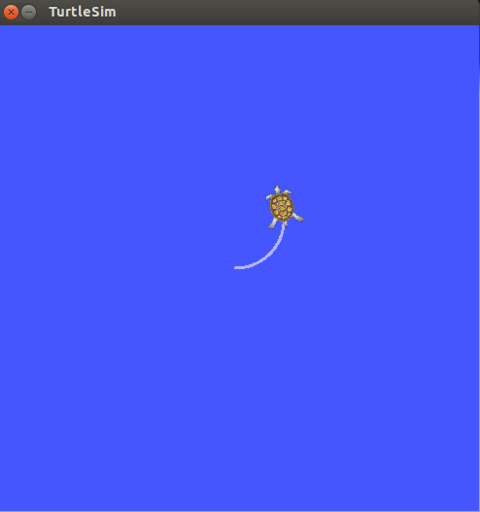
\includegraphics[width=\columnwidth]{pictures/chapter4/pic_04_02.png}
  \caption{配信したメッセージが反映された様子}
\end{figure}

なお、メッセージ型の詳細は、以下のように「rosmsg show [メッセージ名]」で調べることができる。

\begin{lstlisting}[language=ROS]
$ rosmsg show geometry_msgs/Twist
geometry_msgs/Vector3 linear
float64 x
float64 y
float64 z
geometry_msgs/Vector3 angular
float64 x
float64 y
float64 z
\end{lstlisting}

\begin{exercise}[ROSで使用される単位]
単位(unit)はROS規則で取決められており、パッケージ作成時にhttp://www.ros.org/reps/rep-0103.htmlで確認する必要がある。上の例の速度の場合、meter/secやradian/secを使用している。
\end{exercise}


%-------------------------------------------------------------------------------
\subsection{rosservice:ROSサービス情報の確認}

rosserviceは、ROSサービスの情報を確認するためのコマンドである。

\begin{itemize}
\item rosservice [オプション]
\end{itemize}

オプションには、list、info、type、find、uri、args、callなどが指定できる。

rosserviceコマンドの例を示す前に、一度すべてのノードを終了する。次に、それぞれ別のターミナルウィンドウで、次のコマンドを実行して、turtlesim\_nodeとturtle\_teleop\_keyを実行する。

\begin{lstlisting}[language=ROS]
$ roscore
\end{lstlisting}

\begin{lstlisting}[language=ROS]
$ rosrun turtlesim turtlesim_node
\end{lstlisting}

\begin{lstlisting}[language=ROS]
$ rosrun turtlesim turtle_teleop_key
\end{lstlisting}

%-------------------------------------------------------------------------------
\subsubsection{rosservice list:アクティブなサービスの一覧を表示}

rosservice listは使用中のサービスの一覧を表示するコマンドである。

\begin{lstlisting}[language=ROS]
$ rosservice list
/clear
/kill
/reset
/rosout/get_loggers
/rosout/set_logger_level
/spawn
/teleop_turtle/get_loggers
/teleop_turtle/set_logger_level
/turtle1/set_pen
/turtle1/teleport_absolute
/turtle1/teleport_relative
/turtlesim/get_loggers
/turtlesim/set_logger_level
\end{lstlisting}

%-------------------------------------------------------------------------------
\subsubsection{rosservice info [サービス名]:指定されたサービスの情報を表示}

rosservice infoは、実行ノードやPC名、サービス型など、指定されたサービスの詳細な情報を表示するコマンドである。下の例では、/turtle1/set\_penサービスのノード名、URI、サービス型、パラメータを確認できる。

\begin{lstlisting}[language=ROS]
$ rosservice info /turtle1/set_pen
Node: /turtlesim
URI: rosrpc://192.168.4.100:34715
Type: turtlesim/SetPen
Args: r g b width off
\end{lstlisting}

%-------------------------------------------------------------------------------
\subsubsection{rosservice type [サービス名]:指定されたサービスのサービス型を表示}

rosservice typeは、指定したサービスで使用しているサービス型を表示するコマンドである。次の例では、/turtle1/set\_penサービスで使用しているサービスの型がturtlesim/SetPenであることが確認できる。

\begin{lstlisting}[language=ROS]
$ rosservice type /turtle1/set_pen
turtlesim/SetPen
\end{lstlisting}

%-------------------------------------------------------------------------------
\subsubsection{rosservice find [サービス型]:指定したサービス型を使用しているサービスを検索}

rosservice findは指定したサービス型を使用しているサービスを検索し、表示するコマンドである。下の例では、turtlesim/SetPen型を持つサービスが表示されている。

\begin{lstlisting}[language=ROS]
$ rosservice find turtlesim/SetPen
/turtle1/set_pen
\end{lstlisting}

%-------------------------------------------------------------------------------
\subsubsection{rosservice uri [サービス名]:指定されたサービスのROSRPC URIの表示}

rosservice uriは指定したサービスのURIを表示するコマンドである。下の例は、/turtle1/set\_penサービスのROSRPC URIを表示している。

\begin{lstlisting}[language=ROS]
$ rosservice uri /turtle1/set_pen
URI: rosrpc://192.168.4.100:34715
\end{lstlisting}

%-------------------------------------------------------------------------------
\subsubsection{rosservice args [サービス名]:サービスパラメータの表示}

rosservice argsは指定したサービスのパラメータを表示するコマンドである。下の例は、/turtle1/set\_penサービスの各パラメータを表示している様子でありr、g、b、width、offというパラメータが使用されていることが確認できる。

\begin{lstlisting}[language=ROS]
$ rosservice args /turtle1/set_pen
r g b width off
\end{lstlisting}

%-------------------------------------------------------------------------------
\subsubsection{rosservice call [サービス名] [パラメータ]:指定されたサービスのリクエストを実行}

rosservice callは、コマンドラインから指定されたサービスをリクエストするコマンドである。サービスのテストのために使用される便利なコマンドであり、使用頻度は高い。次の例は、/turtle1/set\_penサービスへリクエストするものである。使用された「255 0 0 5 0」の5つの数値はそれぞれ/turtle1/set\_penサービスに使用されているパラメータ(r、g、b、width、off)に対応する。赤を表すrは最大値の255を、g、bはいずれも0とし、widthは5の太さを設定、線の可視化を表すoffは0(false)と設定している。

\begin{lstlisting}[language=ROS]
$ rosservice call /turtle1/set_pen 255 0 0 5 0
\end{lstlisting}

上のコマンドでサービスをリクエストすることで、turtlesimに使用されるペンの特性を変えられる。turtle\_teleop\_keyコマンドで移動した結果、次のように白いペンの色が赤で表示されることが確認できる。

\begin{figure}[htp]
  \centering
  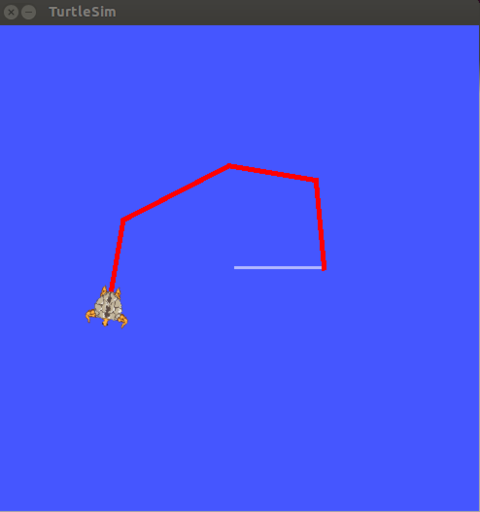
\includegraphics[width=\columnwidth]{pictures/chapter4/pic_04_03.png}
  \caption{rosservice callの例}
\end{figure}

%-------------------------------------------------------------------------------
\subsubsection{rosparam:ROSパラメータ情報の確認と修正}

rosparamは、ROSサービスのパラメータの情報の確認するためのコマンドである。

\begin{itemize}
\item rosparam [オプション]
\end{itemize}

オプションには、list、get、set、dump、load、deleteなどが指定できる。

rosparamコマンドの例を実行する前に、一度すべてのノードを終了する。次に、それぞれ別のターミナルウィンドウで、次のコマンドを実行して、turtlesim\_nodeとturtle\_teleop\_keyを実行する。

\begin{lstlisting}[language=ROS]
$ roscore
\end{lstlisting}

\begin{lstlisting}[language=ROS]
$ rosrun turtlesim turtlesim_node
\end{lstlisting}

\begin{lstlisting}[language=ROS]
$ rosrun turtlesim turtle_teleop_key
\end{lstlisting}

%-------------------------------------------------------------------------------
\subsubsection{rosparam list:パラメータの一覧の表示}

rosparam listは使用中のパラメータの一覧を表示するコマンドである。

\begin{lstlisting}[language=ROS]
$ rosparam list
/background_b
/background_g
/background_r
/rosdistro
/roslaunch/uris/host_192_168_4_100  39536
/rosversion
/run_id
\end{lstlisting}

%-------------------------------------------------------------------------------
\subsubsection{rosparam get [パラメータ名]:パラメータ値の読み込み}

rosparam getは指定したパラメータの値を表示するコマンドである。次の例では、/background\_bパラメータの値を確認できる。

\begin{lstlisting}[language=ROS]
$ rosparam get /background_b
255
\end{lstlisting}

特定のパラメータではなく、すべてのパラメータの値を確認したいときには、オプションで「/」を指定する。

\begin{lstlisting}[language=ROS]
$ rosparam get /
background_b: 255
background_g: 86
background_r: 69
rosdistro: 'indigo'
roslaunch: uris: {host_192_168_4_100  39536: 'http://192.168.4.100:39536/'} rosversion: '1.11.10'
run_id: 93598bxx.44xx.11xx.a0xx.d43d7e97xxxx
\end{lstlisting}

%-------------------------------------------------------------------------------
\subsubsection{rosparam dump [ファイル名]:パラメータ値を指定したファイルに保存}

rosparam dumpは、現在のすべてのパラメータ値を指定したファイルに保存するコマンドである。下の例では、現在のパラメータ値をparameters.yamlのファイルに保存している。毎回使用されるパラメータの値を保存しておき、rosparam loadコマンドで呼び出すことにより、以降の実行時に繰り返し使用できる。

\begin{lstlisting}[language=ROS]
$ rosparam dump ~/parameters.yaml
\end{lstlisting}

%-------------------------------------------------------------------------------
\subsubsection{rosparam set [パラメータ名]:パラメータ値の書き込み}

rosparam dumpは、指定したパラメータに値を設定するコマンドである。下の例では、turtlesimノードの背景色に関するパラメータであるbackground\_bを0に設定している。

\begin{lstlisting}[language=ROS]
$ rosparam set background_b 0
$ rosservice call clear
\end{lstlisting}

これにより、RGBは255、86、69から0、86、69に変更されるため、図4-4の右図のように背景色が濃い緑になる。ただし、turtlesimノードの仕様により、変更を反映するためには、「rosparam set background\_b0」コマンドでパラメータを変更した後、「rosservice call clear」コマンドで画面を更新する必要がある。

\begin{figure}[htp]
  \centering
  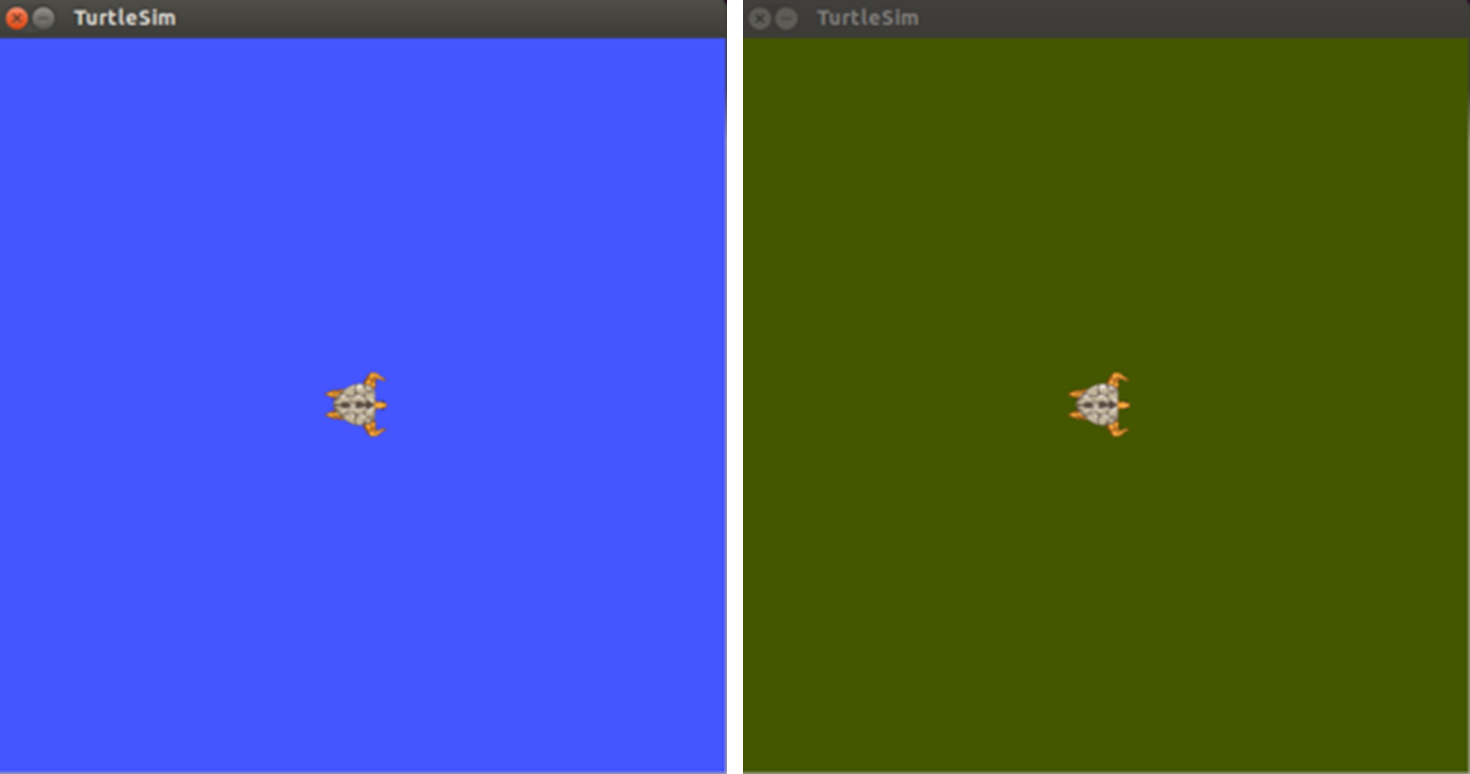
\includegraphics[width=\columnwidth]{pictures/chapter4/pic_04_04.png}
  \caption{rosparam setの例}
\end{figure}

%-------------------------------------------------------------------------------
\subsubsection{rosparam load [ファイル名]:指定したファイルに保存されたパラメータの読み込み}

rospasm loadは、指定したファイルから保存されたパラメータを読み込むコマンドであり、頻繁に使用される。下の例では、「rosparam dump」コマンドとは逆に、parameters.yamlファイルを読み込み、現在のパラメータ値として使用している。このコマンドの後、「rosservice call clear」コマンドを実行し、取得したファイルのパラメータ値を適用する。図4-4で緑になった背景が、「rosparam dump」コマンド実行前の青色の背景に戻ることが分かる。

\begin{lstlisting}[language=ROS]
$ rosparam load ~/parameters.yaml
$ rosservice call clear
\end{lstlisting}

%-------------------------------------------------------------------------------
\subsubsection{rosparam delete [パラメータ名]:パラメータを削除}

rosparam deleteは、指定したパラメータを削除するコマンドである。削除されたパラメータは、rosparam listコマンドで表示されず、パラメータの値は規定値に戻る。

\begin{lstlisting}[language=ROS]
$ rosparam delete /background_b
\end{lstlisting}

%-------------------------------------------------------------------------------
\subsection{rosmsg:ROSメッセージ情報の確認}

rosmsgは、ROSメッセージの情報の確認するためのコマンドである。

\begin{itemize}
\item   rosmsg [オプション]
\end{itemize}

オプションには、list、show、md5、package、packagesなどが指定できる。

rosmsg コマンドの例を示す前に、一度すべてのノードを終了する。次に、それぞれ別のターミナルウィンドウで、次のコマンドを実行して、turtlesim\_nodeとturtle\_teleop\_keyを実行する。

\begin{lstlisting}[language=ROS]
$ roscore
\end{lstlisting}

\begin{lstlisting}[language=ROS]
$ rosrun turtlesim turtlesim_node
\end{lstlisting}

\begin{lstlisting}[language=ROS]
$ rosrun turtlesim turtle_teleop_key
\end{lstlisting}

%-------------------------------------------------------------------------------
\subsubsection{rosmsg list:すべてのメッセージの一覧を表示}

rosmsg listは、インストール済みパッケージのすべてのメッセージを表示するコマンドである。

\begin{lstlisting}[language=ROS]
$ rosmsg list
actionlib/TestAction
actionlib/TestActionFeedback
actionlib/TestActionGoal
actionlib/TestActionResult
actionlib/TestFeedback
actionlib/TestGoal
sensor_msgs/Joy
sensor_msgs/JoyFeedback
sensor_msgs/JoyFeedbackArray
sensor_msgs/LaserEcho
zeroconf_msgs/DiscoveredService
%*〜省略〜*)
\end{lstlisting}

%-------------------------------------------------------------------------------
\subsubsection{rosmsg show [メッセージ名]:指定したメッセージのメッセージ型を表示}

rosmsg showは、指定したメッセージのメッセージ型を表示するコマンドである。下の例では、turtlesim/Poseメッセージのメッセージ型を出力している様子である。float32(浮動小数点型変数)で、x、y、theta、linear\_velocity、angular\_velocityの5つの変数からなるメッセージであることが確認できる。

\begin{lstlisting}[language=ROS]
$ rosmsg show turtlesim/Pose
float32 x
float32 y
float32 theta
float32 linear_velocity
float32 angular_velocity
\end{lstlisting}

%-------------------------------------------------------------------------------
\subsubsection{rosmsg md5 [メッセージ名]:指定したメッセージのmd5sumを表示}

rosmsg md5は、指定したメッセージのmd5sumの値を表示するコマンドである。下の例は、turtlesim/Poseメッセージのmd5sumの値を確認している様子である。メッセージ通信中にMD5問題が発生し、md5sumを確認する必要がある時、使用される。

\begin{lstlisting}[language=ROS]
$ rosmsg md5 turtlesim/Pose
863b248d5016ca62ea2e895ae5265cf9
\end{lstlisting}

%-------------------------------------------------------------------------------
\subsubsection{rosmsg package [パッケージ名]:指定したパッケージで使用されるメッセージの一覧を表示}

rosmsg packageは、指定したパッケージで使用されるメッセージを表示するコマンドである。

\begin{lstlisting}[language=ROS]
$ rosmsg package turtlesim
turtlesim/Color
turtlesim/Pose
\end{lstlisting}

%-------------------------------------------------------------------------------
\subsubsection{rosmsg packages:メッセージを使用しているすべてのパッケージの一覧を表示}

rosmsg packagesは、メッセージを使用しているすべてのパッケージを表示するコマンドである。

\begin{lstlisting}[language=ROS]
$ rosmsg packages
actionlib
actionlib_msgs
actionlib_tutorials
base_local_planner
bond
control_msgs costmap_2d
%*〜省略〜*)
\end{lstlisting}

%-------------------------------------------------------------------------------
\subsection{rossrv:ROSサービス情報の確認}

rossrvは、ROSサービスの情報の確認するためのコマンドである。

\begin{itemize}
\item rossrv [オプション]
\end{itemize}

オプションには、rosmsgと同様に、list、show、md5、package、packagesなどが指定できる。

rossrvコマンドの例を示す前に、一度すべてのノードを終了する。次に、それぞれ別のターミナルウィンドウで、次のコマンドを実行して、turtlesim\_nodeとturtle\_teleop\_keyを実行する。

\begin{lstlisting}[language=ROS]
$ roscore
\end{lstlisting}

\begin{lstlisting}[language=ROS]
$ rosrun turtlesim turtlesim_node
\end{lstlisting}

\begin{lstlisting}[language=ROS]
$ rosrun turtlesim turtle_teleop_key
\end{lstlisting}


%-------------------------------------------------------------------------------
\subsubsection{rossrv list:すべてのサービスの一覧を表示}

rossrv listは、インストール済みパッケージのすべてのサービスを表示するコマンドである。

\begin{lstlisting}[language=ROS]
$ rossrv list
control_msgs/QueryCalibrationState
control_msgs/QueryTrajectoryState
diagnostic_msgs/SelfTest
dynamic_reconfigure/Reconfigure
gazebo_msgs/ApplyBodyWrench
gazebo_msgs/ApplyJointEffort
gazebo_msgs/BodyRequest
gazebo_msgs/DeleteModel
%*〜省略〜*)
\end{lstlisting}

%-------------------------------------------------------------------------------
\subsubsection{rossrv show [サービス名]:指定されたサービスの情報を表示}

rossrv showは、指定したサービスの情報を表示するコマンドである。下の例では、turtlesim/SetPenサービスの情報を出力した例である。uint8(符号なし8ビット整数型変数)でr、g、b、width、offの5つの変数が含まれていることが確認できる。参考までに「---」は、サービスファイルのリクエストとレスポンスを区分する線として使用され、このturtlesim/SetPenサービスはリクエストだけがあり、レスポンスに該当するものがないことが分かる。この部分については、6.3節で詳細に取り上げる。

\begin{lstlisting}[language=ROS]
$ rossrv show turtlesim/SetPen
uint8 r
uint8 g
uint8 b
uint8 width
uint8 off
---
\end{lstlisting}

%-------------------------------------------------------------------------------
\subsubsection{rossrv md5 [サービス名]:指定されたサービスのmd5sumを表示}

rossrv md5は、指定したサービスのmd5sumの値を表示するコマンドである。下の例は、turtlesim/SetPenサービスのmd5sum情報を確認している例である。サービスの使用中にMD5問題が発生した場合、md5sumを確認する必要がある時、使用されるコマンドである。

\begin{lstlisting}[language=ROS]
$ rossrv md5 turtlesim/SetPen
9f452acce566bf0c0954594f69a8e41b
\end{lstlisting}

%-------------------------------------------------------------------------------
\subsubsection{rossrv package [パッケージ名]:指定したパッケージで使用しているサービスの一覧を表示}

rossrv packageは、指定したパッケージで使用されるサービスを表示するコマンドである。

\begin{lstlisting}[language=ROS]
$ rossrv package turtlesim
turtlesim/Kill
turtlesim/SetPen
turtlesim/Spawn
turtlesim/TeleportAbsolute
turtlesim/TeleportRelative
\end{lstlisting}

%-------------------------------------------------------------------------------
\subsubsection{rossrv packages:サービスを使用しているすべてのパッケージの一覧を表示}

rossrv packagesは、サービスを使用しているすべてのパッケージを表示するコマンドである。

\begin{lstlisting}[language=ROS]
$ rossrv packages
control_msgs
diagnostic_msgs
dynamic_reconfigure
gazebo_msgs
map_msgs
nav_msgs
navfn nodelet
roscpp sensor_msgs
std_srvs
tf
tf2_msgs
turtlesim
%*〜省略〜*)
\end{lstlisting}

%-------------------------------------------------------------------------------
\subsection{rosbag:ROSメッセージの記録と再生}

ros bagは、ROSメッセージを記録、再生するためのコマンドである。ROSは、bagという形式でメッセージを保存し、必要なときに再生して、記録した時の状況をそのまま再現できる。

\begin{itemize}
\item rosbag [オプション]
\end{itemize}

オプションには、record、info、play、compress、decompress、filter、reindex bag、check bag、fixなどが指定できる。

rosbagコマンドの例を示す前に、一度すべてのノードを終了する。次に、それぞれ別のターミナルウィンドウで、次のコマンドを実行して、turtlesim\_nodeとturtle\_teleop\_keyを実行する。

\begin{lstlisting}[language=ROS]
$ roscore
\end{lstlisting}

\begin{lstlisting}[language=ROS]
$ rosrun turtlesim turtlesim_node
\end{lstlisting}

\begin{lstlisting}[language=ROS]
$ rosrun turtlesim turtle_teleop_key
\end{lstlisting}


%-------------------------------------------------------------------------------
\subsubsection{rosbag record [オプション] [トピック名]:指定されたトピックのメッセージをbagファイルに記録}

rosbag recordは、すべてのトピック、あるいは指定したトピックのメッセージをファイルに記録するコマンドである。
まず、rostopic listコマンドを使用し、使用されているトピックを確認する。

\begin{lstlisting}[language=ROS]
$ rostopic list
/rosout
/rosout_agg
/turtle1/cmd_vel
/turtle1/color_sensor
/turtle1/pose
\end{lstlisting}

次に、使用しているトピックの中から、記録するトピックとして/turtle1/cmd\_velトピックを指定し、bagの記録を開始する。この際、「-O」のオプションで保存ファイル名を指定できる。下の例ではmsglog.bagに保存する。その後、turtle\_teleop\_keyノードでキーボードの矢印キーで亀を移動させると、オプションで指定された/turtle1/cmd\_velトピックが記録される。また、<Ctrl>+<C>を押して記録を終了すると、以下のようにmsglog.bagファイルが生成される。

\begin{lstlisting}[language=ROS]
$ rosbag record -O msglog.bag /turtle1/cmd_vel
[INFO] [1423029313.526437636]: Subscribing to /turtle1/cmd_vel
[INFO] [1423029313.534906460]: Recording to msglog.bag.
\end{lstlisting}

特定のトピックではなく、すべてのトピックを同時に記録したい場合は、以下のようにオプションの「-a」を付ける。

\begin{lstlisting}[language=ROS]
$ rosbag record -a -O msglog.bag
[INFO] [1423029391.499585832]: Recording to msglog.bag.
[INFO] [1423029391.500622809]: Subscribing to /turtle1/color_sensor
[INFO] [1423029391.507350765]: Subscribing to /turtle1/cmd_vel
[INFO] [1423029391.514320943]: Subscribing to /rosout
[INFO] [1423029391.528439120]: Subscribing to /rosout_agg
[INFO] [1423029391.547867201]: Subscribing to /turtle1/pose
\end{lstlisting}

%-------------------------------------------------------------------------------
\subsubsection{rosbag info [ファイル名]:bagファイルの情報を確認}

rosbag infoは、記録したbagファイルの情報を表示するコマンドである。下の例では、記録した/turtle1/cmd\_velトピックのbagファイルが、合計167個のメッセージの記録で構成されていることや、使用されたメッセージの型、パス、バージョン、記録時間などの情報が確認できる。

\begin{lstlisting}[language=ROS]
$ rosbag info msglog.bag
path: msglog.bag
version: 2.0
duration: 12.7s
start: Feb 04 2015 14:55:15.33 (1423029315.33)
end: Feb 04 2015 14:55:28.04 (1423029328.04)
size: 22.5 KB
messages: 167
compression: none [1/1 chunks]
types: geometry_msgs/Twist [9f195f881246fdfa2798d1d3eebca84a]
topics: /turtle1/cmd_vel
167 msgs : geometry_msgs/Twist
\end{lstlisting}

%-------------------------------------------------------------------------------
\subsubsection{rosbag play [ファイル名]:指定されたbagファイルを再生}

rosbag playは、記録したbagファイルを再生するコマンドである。下の例は、上のrosbag recordコマンドの説明で記録したmsglog.bagを再生したものであり、記録時の/turtle1/cmd\_velメッセージがそのまま再生され、画面上のカメが動く様子を確認できる。ただし、turtlesim\_nodeを再起動し、ロボット軌跡とロボットの位置を初期化する必要がある。問題なければ、図4-5のように、rosbag recordで記録した時と同じ軌跡を得ることができる。

\begin{lstlisting}[language=ROS]
$ rosbag play msglog.bag
[INFO] [1423029542.171454338]: Opening msglog.bag
Waiting 0.2 seconds after advertising topics... done.
Hit space to toggle paused, or 's' to step.
[RUNNING]  Bag Time: 1423029315.327811  Duration: 0.000000 / 12.713
[RUNNING]  Bag Time: 1423029315.327889  Duration: 0.000078 / 12.713
%*〜省略〜*)
\end{lstlisting}

\begin{figure}[htp]
  \centering
  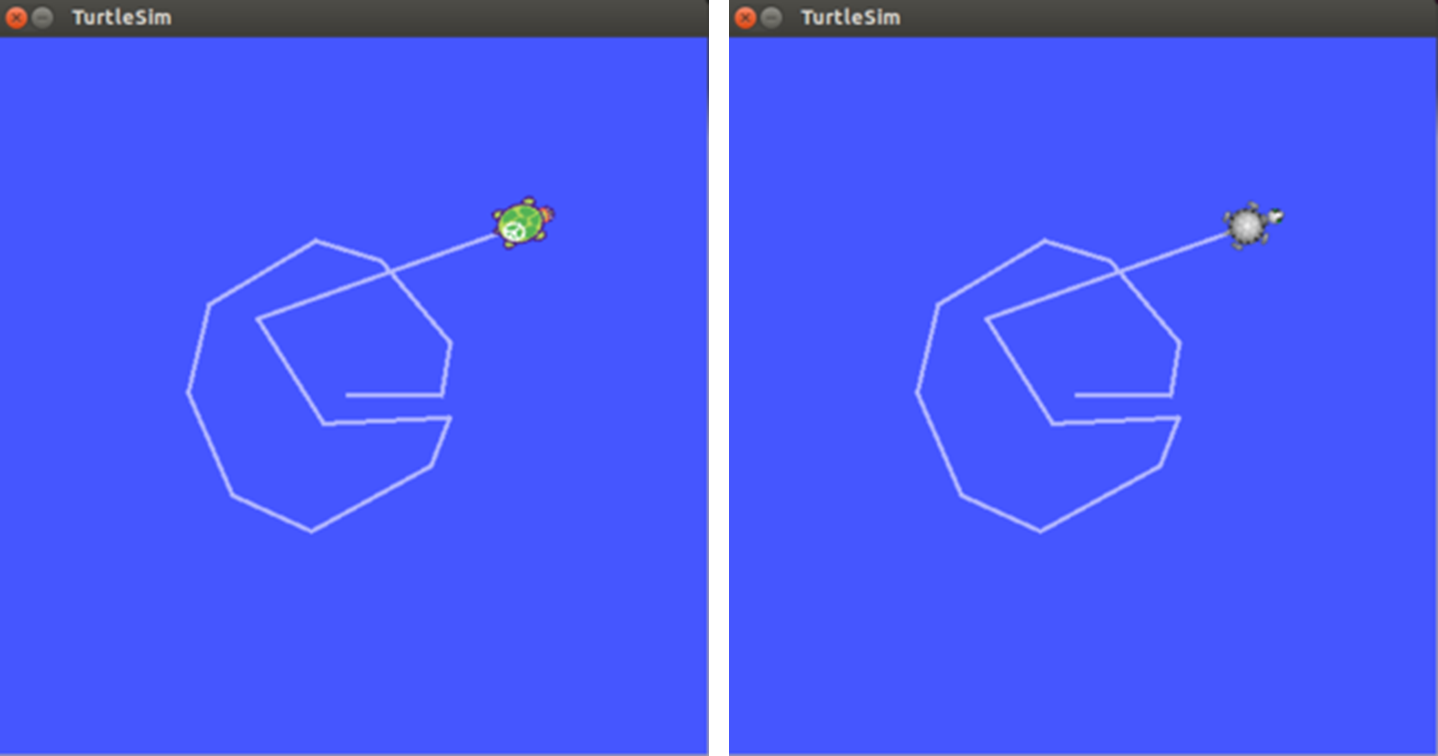
\includegraphics[width=\columnwidth]{pictures/chapter4/pic_04_05.png}
  \caption{rosbag playの例(左:記録時、右:再生時)}
\end{figure}

%-------------------------------------------------------------------------------
\subsubsection{rosbag compress [ファイル名]:指定されたbagファイルを圧縮}

rosbag compressは、記録したbagファイルを圧縮するコマンドである。bagファイルに長時間記録すると、bagファイルのサーズが大きくなる。そこで、rosbag compressコマンドでbagファイルを圧縮して、ファイルサイズを小さくできる。

\begin{lstlisting}[language=ROS]
$ rosbag compress msglog.bag
msglog.bag  100%   15.8 KB 00:00
\end{lstlisting}

上の例では、bagファイルが次のように3分の1に縮小される。圧縮前の元ファイルは、origという拡張子が追加され、別に保存されている。

\begin{lstlisting}[language=ROS]
msglog.bag 8.5kB
msglog.orig.bag 23.0kB
\end{lstlisting}

%-------------------------------------------------------------------------------
\subsubsection{rosbag decompress [ファイル名]:指定されたbagファイルを圧縮解除}

rosbag decompressは、rosbag compressコマンドで圧縮されたファイルを圧縮前の状態に戻すコマンドである。

\begin{lstlisting}[language=ROS]
$ rosbag decompress msglog.bag
msglog.bag  100%  15.8 KB 00:00
\end{lstlisting}

%-------------------------------------------------------------------------------
\subsubsection{rosbag filter [入力ファイル] [出力ファイル] [オプション]:bagファイルの再作成}

rosbag filterは、作成済みのbagファイルから、指定されたトピックのみを残して、新しいbagファイルを作成するコマンドである。

rosbag filterコマンドの例を実行する前に、一度すべてのノードを終了する。次に、それぞれ別のターミナルウィンドウで、次のコマンドを実行して、turtlesim\_nodeとturtle\_teleop\_keyを実行する。

\begin{lstlisting}[language=ROS]
$ roscore
\end{lstlisting}

\begin{lstlisting}[language=ROS]
$ rosrun turtlesim turtlesim_node
\end{lstlisting}

\begin{lstlisting}[language=ROS]
$ rosrun turtlesim turtle_teleop_key
\end{lstlisting}

次に、rosbag recordコマンドを実行し、msglog.bagファイルに全てのトピックを記録する。

\begin{lstlisting}[language=ROS]
$ rosbag record -O msglog.bag -a
\end{lstlisting}

turtle\_teleop\_keyを実行したターミナルで矢印キーを操作し、亀を移動させる。その後、<Ctrol>+<C>でrosbag recordコマンドを終了する。

記録したmsglog.bagをrosbag infoコマンドで確認すると、以下のように/rosout, /turtle1/cmd\_vel, /turtle1/color\_sensor, /turtle1/pose トピックが記録されていることがわかる。

\begin{lstlisting}[language=ROS]
$ rosbag info msglog.bag
path:        msglog.bag
version:     2.0
duration:    12.6s
start:       Jul 16 2015 19:08:28.26 (1437041308.26)
end:         Jul 16 2015 19:08:40.88 (1437041320.88)
size:        127.6 KB
messages:    1645
compression: none [1/1 chunks]
types:       geometry_msgs/Twist [9f195f881246fdfa2798d1d3eebca84a]
             rosgraph_msgs/Log   [acffd30cd6b6de30f120938c17c593fb]
             turtlesim/Color     [353891e354491c51aabe32df673fb446]
             turtlesim/Pose      [863b248d5016ca62ea2e895ae5265cf9]
topics:      /rosout                   4 msgs    : rosgraph_msgs/Log   (2 connections)
             /turtle1/cmd_vel         92 msgs    : geometry_msgs/Twist
             /turtle1/color_sensor   775 msgs    : turtlesim/Color
             /turtle1/pose           774 msgs    : turtlesim/Pose
\end{lstlisting}

次に、rosbag filterコマンドにより、/turtle1/cmd\_velトピックのみを残して、他のトピックを削除する。以下では、出力ファイルをonly\_cmd\_vel.bagとしている。

\begin{lstlisting}[language=ROS]
$ rosbag filter msglog.bag only_cmd_vel.bag "topic == '/turtle1/cmd_vel'"
\end{lstlisting}

rosbag infoコマンドによりonly\_cmd\_vel.bagファイルを確認すると、/turtle1/cmd\_velトピックのみが含まれていることがわかる。このようにrosbag filterコマンドは、指定されたトピックのみを残して、新しいbagファイルを作成するために使用される。

\begin{lstlisting}[language=ROS]
$ rosbag info only_cmd_vel.bag
path:    only_cmd_vel.bag
version: 2.0
size:    4.0 KB
rt@rt:~$ rosbag info only_cmd_vel.bag
path:        only_cmd_vel.bag
version:     2.0
duration:    5.9s
start:       Jul 16 2015 19:08:32.09 (1437041312.09)
end:         Jul 16 2015 19:08:38.03 (1437041318.03)
size:        14.7 KB
messages:    92
compression: none [1/1 chunks]
types:       geometry_msgs/Twist [9f195f881246fdfa2798d1d3eebca84a]
topics:      /turtle1/cmd_vel   92 msgs    : geometry_msgs/Twist
\end{lstlisting}

複数のトピックを残す場合は、以下のようにトピック名を続けて指定する。

\begin{lstlisting}[language=ROS]
$ rosbag filter msglog.bag only_cmd_vel.bag "topic == '/turtle1/cmd_vel' or topic == '/turtle1/pose'"
\end{lstlisting}

%-------------------------------------------------------------------------------
\subsubsection{rosbag reindex [ファイル名]:bagファイルの再インデックス}

rosbag reindex は、bagファイルに問題があり再生できない場合、再インデックスによりbagファイルを修復するコマンドである。元のbagファイルはmsglog.orig.bagとして保存され、修復されたbagファイルは同じ名前で上書きされる。

\begin{lstlisting}[language=ROS]
$ rosbag reindex msglog.bag
 msglog.bag                       100%            123.8 KB 00:00
\end{lstlisting}

%-------------------------------------------------------------------------------
\subsubsection{rosbag check bag [ファイル名]:bagファイルの再生確認}

rosbag check bagは、指定されたbagファイルが現在のROSシステムで再生できるかを確認するコマンドである。現在のROSシステムで再生できる場合、以下のように表示される。

\begin{lstlisting}[language=ROS]
$ rosbag check msglog.bag
Bag file is up to date.
\end{lstlisting}

%-------------------------------------------------------------------------------
\subsubsection{rosbag fix [入力ファイル] [出力ファイル] [オプション]:bagファイルのバージョン変更}

rosbag fixは、ROSのバージョンが異なり現在のROSシステムでは再生が不可能なbagファイルを、再生できる形式に変換するコマンドである。

\begin{lstlisting}[language=ROS]
$ rosbag fix msglog.bag repaired_msglog.bag
Bag migrated successfully.
\end{lstlisting}

%-------------------------------------------------------------------------------
\section{ROS catkinコマンド}\index{ROS catkinコマンド}

ROS catkinは、catkinビルドシステムを用いてパッケージをビルドする際に使用される。

\vspace{\baselineskip}
\noindent
\begin{description}
\item[catkin\_create\_pkg](★★★):catkinビルドシステムでパッケージを自動生成
\item[catkin\_make](★★★):catkinビルドシステムのビルド命令
\item[catkin\_eclipse](★★☆):catkinビルドシステムで生成したパッケージをEclipseで使用できるように変更
\item[catkin\_prepare\_release](★★☆):リリース準備するときに使用されるchangelog整理とバージョンのタグ管理
\item[catkin\_generate\_changelog](★★☆):リリースするときCHANGELOG.rstファイルの作成又は更新
\item[catkin\_init\_workspace](★☆☆):catkinビルドシステムの作業フォルダの初期化
\item[catkin\_find](☆☆☆):catkin検索
\end{description}

%-------------------------------------------------------------------------------
\subsection{catkin\_create\_pkg:catkinビルドシステムでパッケージを自動生成}

catkin\_create\_pkgはCMakeLists.txtとpackage.xmlを含む空のパッケージを生成するコマンドである。詳しい使用方法は3.4.1項を参照のこと。

\begin{itemize}
\item catkin\_create\_pkg <パッケージ名> [依存パッケージ1] [依存パッケージ2] …
\end{itemize}

catkin\_create\_pkgの使用例を下に示す。

\begin{lstlisting}[language=ROS]
$ catkin_create_pkg my_package roscpp std_msgs
\end{lstlisting}

%-------------------------------------------------------------------------------
\subsection{catkin\_make:catkinビルドシステムのビルド命令}

catkin\_makeはユーザーが作成したパッケージまたはダウンロードしたパッケージをビルドするコマンドである。

\begin{itemize}
\item  catkin\_make
\end{itemize}

~/catkin\_ws/srcフォルダにある全てのパッケージをビルドする例を示す。

\begin{lstlisting}[language=ROS]
$ cd ~/catkin_ws
$ catkin_make
\end{lstlisting}

全てのパッケージではなく、一部のパッケージのみビルドする場合は、以下ように--pkg [パッケージ名] オプションを指定して実行する。

\begin{lstlisting}[language=ROS]
catkin_make --pkg user_ros_tutorials
\end{lstlisting}

%-------------------------------------------------------------------------------
\subsection{catkin\_eclipse:Eclipseを使用したパッケージの管理}

catkin\_eclipseは、統合開発環境(IDE)の一つであるEclipseを用いて、ユーザーが作成したパッケージを管理し、プログラミングを行う環境を構築するコマンドである。

\begin{itemize}
\item catkin\_eclipse
\end{itemize}

このコマンドを実行すると~/catkin\_ws/build/.cproject、~/catkin\_ws/build/.projectなど、Eclipse用のプロジェクトファイルが生成される。Eclipse のメニューから「Makefile Project with Existing Code」を選択し、「~/catkin\_ws/build/」を選択すると、~/catkin\_ws/srcにある全パッケージをEclipseで管理できる。

\begin{lstlisting}[language=ROS]
$ cd ~/catkin_ws
$ catkin_eclipse
\end{lstlisting}

%-------------------------------------------------------------------------------
\subsection{catkin\_generate\_changelog:CHANGELOG.rstファイルの作成}

catkin\_generate\_changelogは、パッケージのバージョンアップ時に変更点を記述するCHANGELOG.rstファイルを作成するコマンドである。

\begin{itemize}
\item catkin\_generate\_changelog
\end{itemize}

%-------------------------------------------------------------------------------
\subsection{catkin\_prepare\_release:リリース準備するときに使用されるchangelog整理とバージョンのタグ管理}

catkin\_prepare\_releaseは、catkin\_generate\_changelogコマンドで作成されたCHANGELOG.rstを更新するとき使用されるコマンドである。

\begin{itemize}
\item catkin\_prepare\_release
\end{itemize}

catkin\_generate\_changelogとcatkin\_prepare\_releaseコマンドは、作成したパッケージをROSレポジトリ注3に登録する時や、登録されたパッケージのバージョンアップの際に使用されるコマンドである。

%-------------------------------------------------------------------------------
\subsection{catkin\_init\_workspace:catkinビルドシステムの作業フォルダの初期化}

catkin\_init\_workspaceはユーザーの作業フォルダ(~/catkin\_ws/src)の初期化コマンドである。

\begin{itemize}
\item catkin\_init\_workspace
\end{itemize}

2.1.1項で説明したように、このコマンドはROSインストールの後に一度だけ行えばよい。

\begin{lstlisting}[language=ROS]
$ cd ~/catkin_ws/src
$ catkin_init_workspace
\end{lstlisting}

%-------------------------------------------------------------------------------
\subsection{catkin\_find:ワークスペースの検索}

catkin\_findはプロジェクト毎に作業フォルダを表示するコマンドである。

\begin{itemize}
\item  catkin\_find [パッケージ名]
\end{itemize}

catkin\_findコマンドを実行すると、使用している全ての作業フォルダを調べることができる。また、「catkin\_find パッケージ名」とすると、オプションで指定したパッケージに関連する作業フォルダが表示される。

\begin{lstlisting}[language=ROS]
$ catkin_find
/home/rt/catkin_ws/devel/include
/home/rt/catkin_ws/devel/lib
/home/rt/catkin_ws/devel/share
/opt/ros/indigo/bin
/opt/ros/indigo/etc
/opt/ros/indigo/include
/opt/ros/indigo/lib
/opt/ros/indigo/share
\end{lstlisting}

\begin{lstlisting}[language=ROS]
$ catkin_find turtlesim
/opt/ros/indigo/include/turtlesim
/opt/ros/indigo/lib/turtlesim
/opt/ros/indigo/share/turtlesim
\end{lstlisting}

%-------------------------------------------------------------------------------
\section{ROSパッケージコマンド}\index{ROSパッケージコマンド}
ROS パッケージは、パッケージの情報表示や関連パッケージのインストールなど、ROSのパッケージ操作に使用される。

\vspace{\baselineskip}
\noindent
\begin{description}
\item[rospack](★★☆)ros+pack(age):指定したROSパッケージに関連する情報を表示
\item[rosinstall](★☆☆)ros+install:ROS追加パッケージの自動インストール
\item[rosdep](★☆☆)ros+dep(endencies):ROSパッケージの依存関係ファイルのインストール
\item[roslocate](☆☆☆)ros+locate:ROSパッケージの情報表示
\item[roscreate-pkg](☆☆☆)ros+create-pkg:ROSパッケージの自動生成(旧rosbuildシステムで使用)
\item[rosmake](☆☆☆)ros+make:ROSパッケージをビルド(旧rosbuildシステムで使用)
\end{description}

%-------------------------------------------------------------------------------
\subsection{rospack:指定したROSパッケージに関連する情報を表示}

rospackは指定したROSパッケージに関連する保存先、依存関係、全パッケージのリストなどの情報を表示するコマンドである。

\begin{itemize}
\item  rospack [オプション] [パッケージ名]
\end{itemize}

オプションには、find、list、depends-on、depends、profileを指定できる。

以下の例のようにrospack findコマンドに続いてパッケージ名を指定すると、そのパッケージの保存先が表示される。

\begin{lstlisting}[language=ROS]
$ rospack find turtlesim
/opt/ros/indigo/share/turtlesim
\end{lstlisting}

rospack listコマンドは、PCにある全パッケージを表示するコマンドである。rospack listコマンドとLinuxの検索コマンドであるgrepを組み合わせすると、簡単にパッケージを探すことができる。例えば以下の例のように「rospack list | grep turtle」を実行すると、全てのパッケージのなかからturtleに関連するパッケージのみ表示される。

\begin{lstlisting}[language=ROS]
$ rospack list
actionlib /opt/ros/indigo/share/actionlib
actionlib_msgs /opt/ros/indigo/share/actionlib_msgs
actionlib_tutorials /opt/ros/indigo/share/actionlib_tutorials
amcl /opt/ros/indigo/share/amcl
angles /opt/ros/indigo/share/angles
ar_track_alvar /opt/ros/indigo/share/ar_track_alvar
\end{lstlisting}

\begin{lstlisting}[language=ROS]
$ rospack list | grep turtle
turtle_actionlib /opt/ros/indigo/share/turtle_actionlib
turtle_concert /opt/ros/indigo/share/turtle_concert
turtle_tf /opt/ros/indigo/share/turtle_tf
\end{lstlisting}

rospack depends-onコマンドの後に パッケージ名を指定すると、指定したパッケージを利用しているパッケージの一覧が表示される。

\begin{lstlisting}[language=ROS]
$ rospack depends-on turtlesim
turtle_tf
turtle_tf2
turtle_actionlib
turtle_concert
concert_service_turtlesim
\end{lstlisting}

rospack dependsコマンドの後に パッケージ名を指定すると、指定したパッケージの実行に必要な依存パッケージの一覧が表示される。

\begin{lstlisting}[language=ROS]
$ rospack depends turtlesim
cpp_common
rostime
roscpp_traits
roscpp_serialization
genmsg
genpy
message_runtime
std_msgs
geometry_msgs
catkin
gencpp
genlisp
message_generation
rosbuild
rosconsole
rosgraph_msgs
xmlrpcpp
roscpp
rospack
roslib
std_srvs
\end{lstlisting}

rospack profileコマンドは、パッケージが保存されている「/opt/ros/indigo/share」や「~/catkin\_ws/src」などの作業フォルダやパッケージの情報を確認し、パッケージのインデックスを再構築するコマンドである。新しく追加したパッケージが「roscd」などで反映されないときに実行する。

\begin{lstlisting}[language=ROS]
$ rospack profile
Full tree crawl took 0.048631 seconds.
Directories marked with (*) contain no manifest. You may want to delete these directories.
To get just of list of directories without manifests, re-run the profile with --zombie-only
0.032159   /opt/ros/indigo/share
0.015752   /home/rt/catkin_ws/src
%*〜省略〜*)
\end{lstlisting}

%-------------------------------------------------------------------------------
\subsection{rosinstall:ROS追加パッケージの自動インストール}

rosinstallは、SVN, Mercurial, git, Bazaarなどの様々なソース・コード・マネージメント(SCM)で管理されているROSのパッケージを、自動的にインストールあるいはアップデートするコマンドである。

\begin{itemize}
\item rosinstall
\end{itemize}

2.1.1項のようにインストールしておくと、その後はパッケージをアップデートすると自動的に必要なパッケージがインストール、あるいはアップデートされる。

%-------------------------------------------------------------------------------
\subsection{rosdep:ROSパッケージの依存関係ファイルのインストール}

rosdepは指定したパッケージの依存関係ファイルをインストールするコマンドである。

\begin{itemize}
\item  rosdep [オプション]
\end{itemize}

オプションには、check、install、init、updateなどが指定できる。

下の例のように、「rosdep check パッケージ名」を実行すると、指定したパッケージの依存関係を確認する。「rosdep install パッケージ名」を実行すると、指定したパッケージの依存パッケージがインストールされる。他にも「rosdep init」や「rosdep update」もあるが、これらは2.1 節を参考にしてほしい。

\begin{lstlisting}[language=ROS]
$ rosdep check turtlesim
All system dependencies have been satisified
\end{lstlisting}

\begin{lstlisting}[language=ROS]
$ rosdep install turtlesim
All required rosdeps installed successfully
\end{lstlisting}

%-------------------------------------------------------------------------------
\subsection{roslocate:ROSパッケージの情報表示}

roslocateは、パッケージが使用しているROSのバージョン、SCMの種類、レポジトリ先など、パッケージに関連した情報を表示するコマンドである。

\begin{itemize}
\item roslocate [オプション] [パッケージ名]
\end{itemize}

オプションには、info、vcs、type、uri、repoなどが指定できるが、ここではそれらを全て一覧で表示するinfoオプションの例を示す。

\begin{lstlisting}[language=ROS]
$ roslocate info turtlesim
Using ROS_DISTRO: indigo
- git:
    local-name: turtlesim
    uri: https://github.com/ros/ros_tutorials.git
    version: indigo-devel
\end{lstlisting}

%-------------------------------------------------------------------------------
\subsection{roscreate-pkg:ROSパッケージの自動生成(旧rosbuildシステムで使用)}

roscreate-pkgはcatkin\_create\_pkgコマンドと同様にパッケージを自動生成するコマンドである。

\begin{itemize}
\item  rosbuild [パッケージ名]
catkinビルドシステム以前のrosbuildシステムのためのコマンドであり、最近は使われない。
\end{itemize}

%-------------------------------------------------------------------------------
\subsection{rosmake:ROSパッケージをビルド(旧rosbuildシステムで使用)}

rosmakeは「catkin\_make」と同様にパッケージをビルドするコマンドである。

\begin{itemize}
\item  rosmake
\end{itemize}
catkinビルドシステム以前のrosbuildシステムのためのコマンドであり、最近は使われない。

% 注1  http://wiki.ros.org/ROS/CommandLineTools
% 注2  https://github.com/ros/ros_tutorials/blob/indigo-devel/turtlesim/tutorials/teleop_turtle_key.cpp
% 注3  rosdistroレポジトリ https://github.com/robotpilot/rosdistro




%-------------------------------------------------------------------------------

% !TEX root = ./rosbook_jp.tex
%-------------------------------------------------------------------------------
\chapterimage{chapter_head_5.pdf}

%-------------------------------------------------------------------------------
\chapter{ROSツール}\index{ROSツール}

本章では、ROSを用いたプログラム開発で利用できる便利なツールを紹介する。この章で説明するツールは、次の通りである。

\begin{itemize}
\item [RViz] 3次元可視化ツール
\item [rqt] QtベースのROS GUI開発ツール
\item [rqt\_image\_view] カメラ映像を表示するツール
\item [rqt\_graph] ノードとメッセージ間の関係をグラフで表示するツール
\item [rqt\_plot] 2次元データのプロットツール
\item [rqt\_bag] GUIベースのbagデータ分析ツール
\end{itemize}

%-------------------------------------------------------------------------------
\section{3次元可視化ツール RViz}\index{3次元可視化ツール RViz}

RVizは、ROSの3次元可視化ツールである。RVizはROSネットワーク上のデータを3次元的に可視化でき、センサの計測データの確認や3次元コンピュータグラフィックスによるロボットの動作確認などに利用できる。例えば、レーザーレンジファインダー(LRF、Laser Range Finder)などの距離センサから得られる距離データ、KinectやXtionなどの3次元センサから得られる点群データ(PCD、Point Cloud Data)、カメラから取得したカラー画像などが表示できる。図5-1から図5-4は、それぞれ超音波センサ、Kinect、LRF、Xtionのデータを3次元的に可視化した例である。

RVizでは、あらかじめ用意された多くの画面設定(ディスプレイ)から適切なものを選択することで、多様な情報が表示できる。例えば、ディスプレイの一つであるInteractive Markersを使用すると、対象物の可視化と同時に、指定した対象物の位置・姿勢をユーザーが自由に変えることができ、インタラクティブなノードとユーザー間の情報(ロボットアームの位置・姿勢や目的地の位置・姿勢など)のやりとりが可能になる。また、3次元モデルの記述法であるURDF(Unified Robot Description Format)フォーマットでロボットを定義し、ファイルに保存しておけば、RVizはそのファイルを読み込み、3次元コンピュータグラフィックスでロボットを表示できる。さらに、モデルに関節自由度や移動自由度を定義しておけば、ロボットの位置や姿勢を変更でき、シミュレーションや実時間でのロボットの動作確認に利用できる。


\begin{figure}[h]
  \centering
  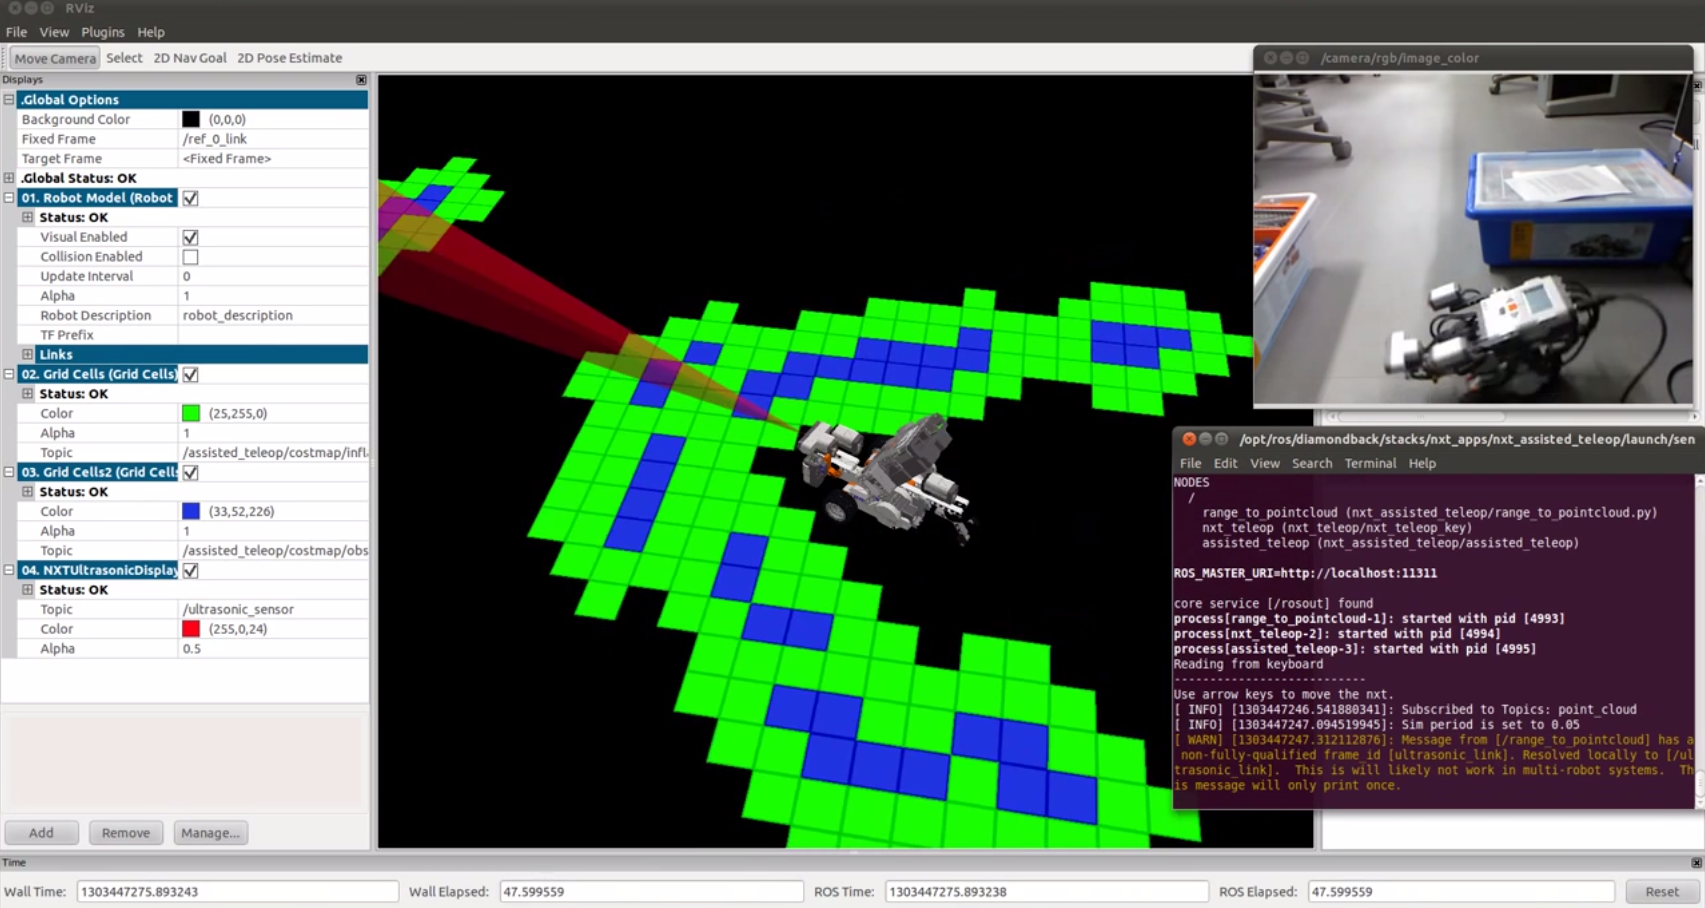
\includegraphics[width=\columnwidth]{pictures/chapter5/pic_05_01.png}
  \caption{RViz使用例1:LEGOロボットと超音波センサを用いた簡単なマップの作成の例}
\end{figure}

\begin{figure}[h]
  \centering
  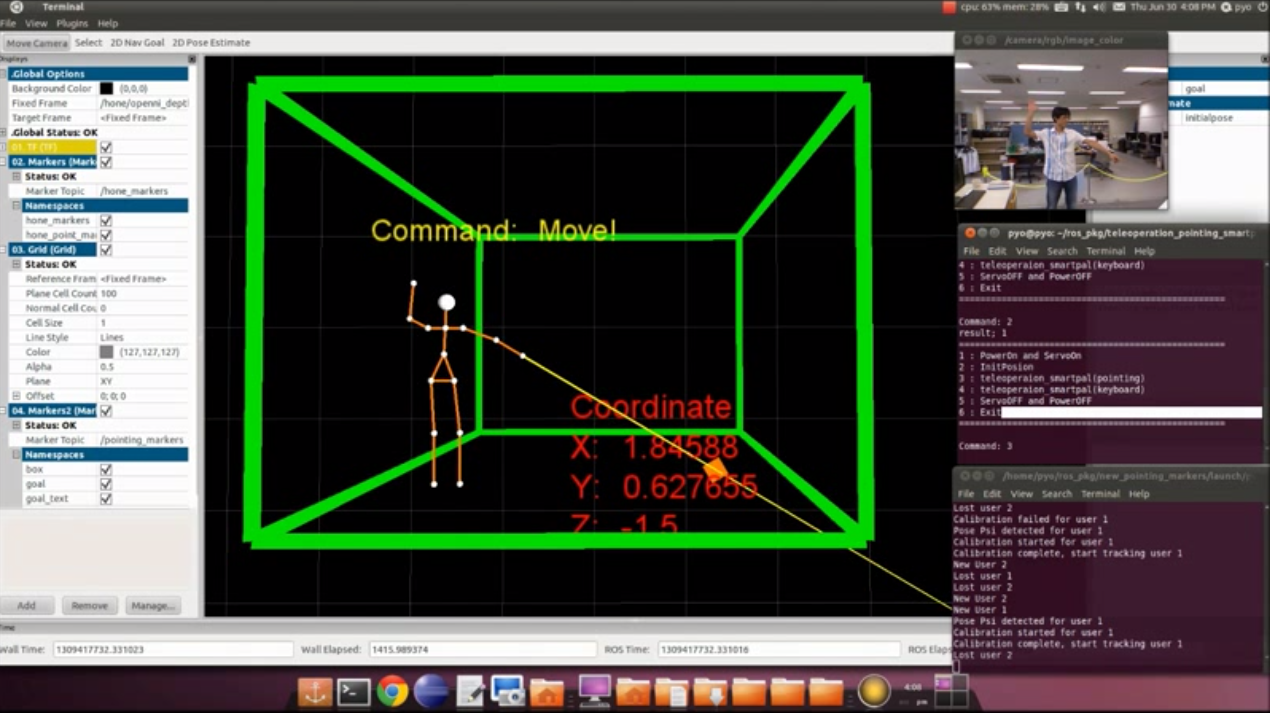
\includegraphics[width=\columnwidth]{pictures/chapter5/pic_05_02.png}
  \caption{RViz使用例2:Kinectから人の骨格を取得し、ロボットを制御している例}
\end{figure}

\begin{figure}[h]
  \centering
  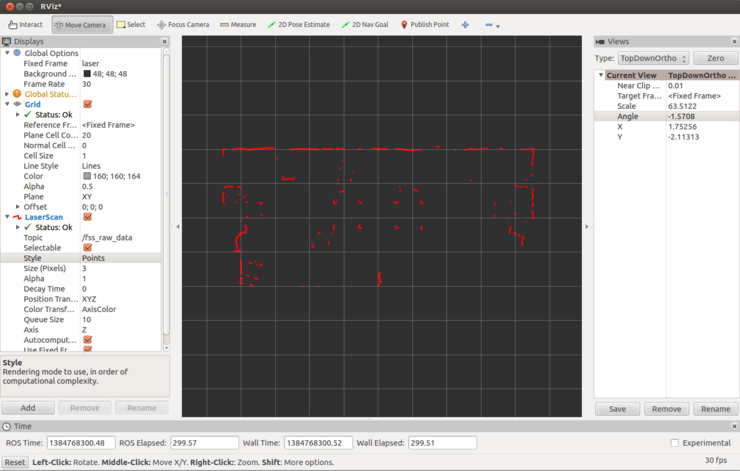
\includegraphics[width=\columnwidth]{pictures/chapter5/pic_05_03.png}
  \caption{RViz使用例3:LRFを用いた距離計測の例}
\end{figure}

\begin{figure}[h]
  \centering
  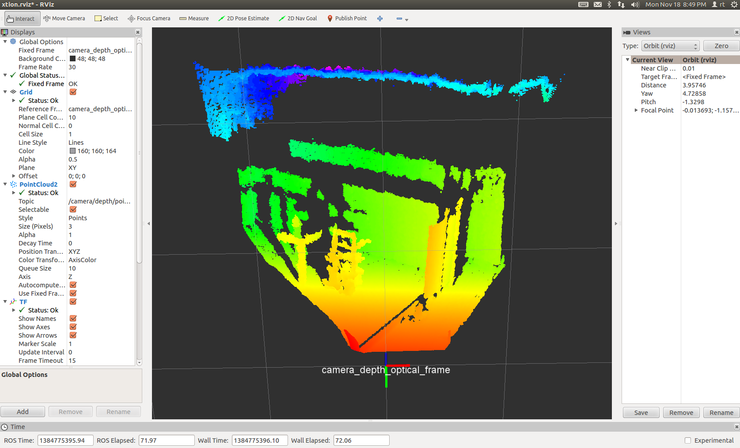
\includegraphics[width=\columnwidth]{pictures/chapter5/pic_05_04.png}
  \caption{RViz使用例4:Xtionセンサから取得した3次元距離値の例}
\end{figure}

%-------------------------------------------------------------------------------
\subsection{RVizのインストールと実行}

RVizは、ROSを第2章で紹介した方法に従い「sudo apt-get install ros-indigo-desktop-full」でインストールすると、自動的にインストールされる。もし上記以外の方法によりRVizがインストールされていない場合は、次のコマンドでインストールする。

\vspace{\baselineskip}
\begin{lstlisting}[language=ROS]
$ sudo apt-get install ros-indigo-rviz
\end{lstlisting}

RVizの実行コマンドは、次のとおりである。ただし、roscoreが実行されている必要がある。

\vspace{\baselineskip}
\begin{lstlisting}[language=ROS]
$ rosrun rviz rviz
\end{lstlisting}

%-------------------------------------------------------------------------------
\subsection{RVizの画面構成}

RVizの画面構成について、図5-5を用いて説明する。

\begin{figure}[h]
  \centering
  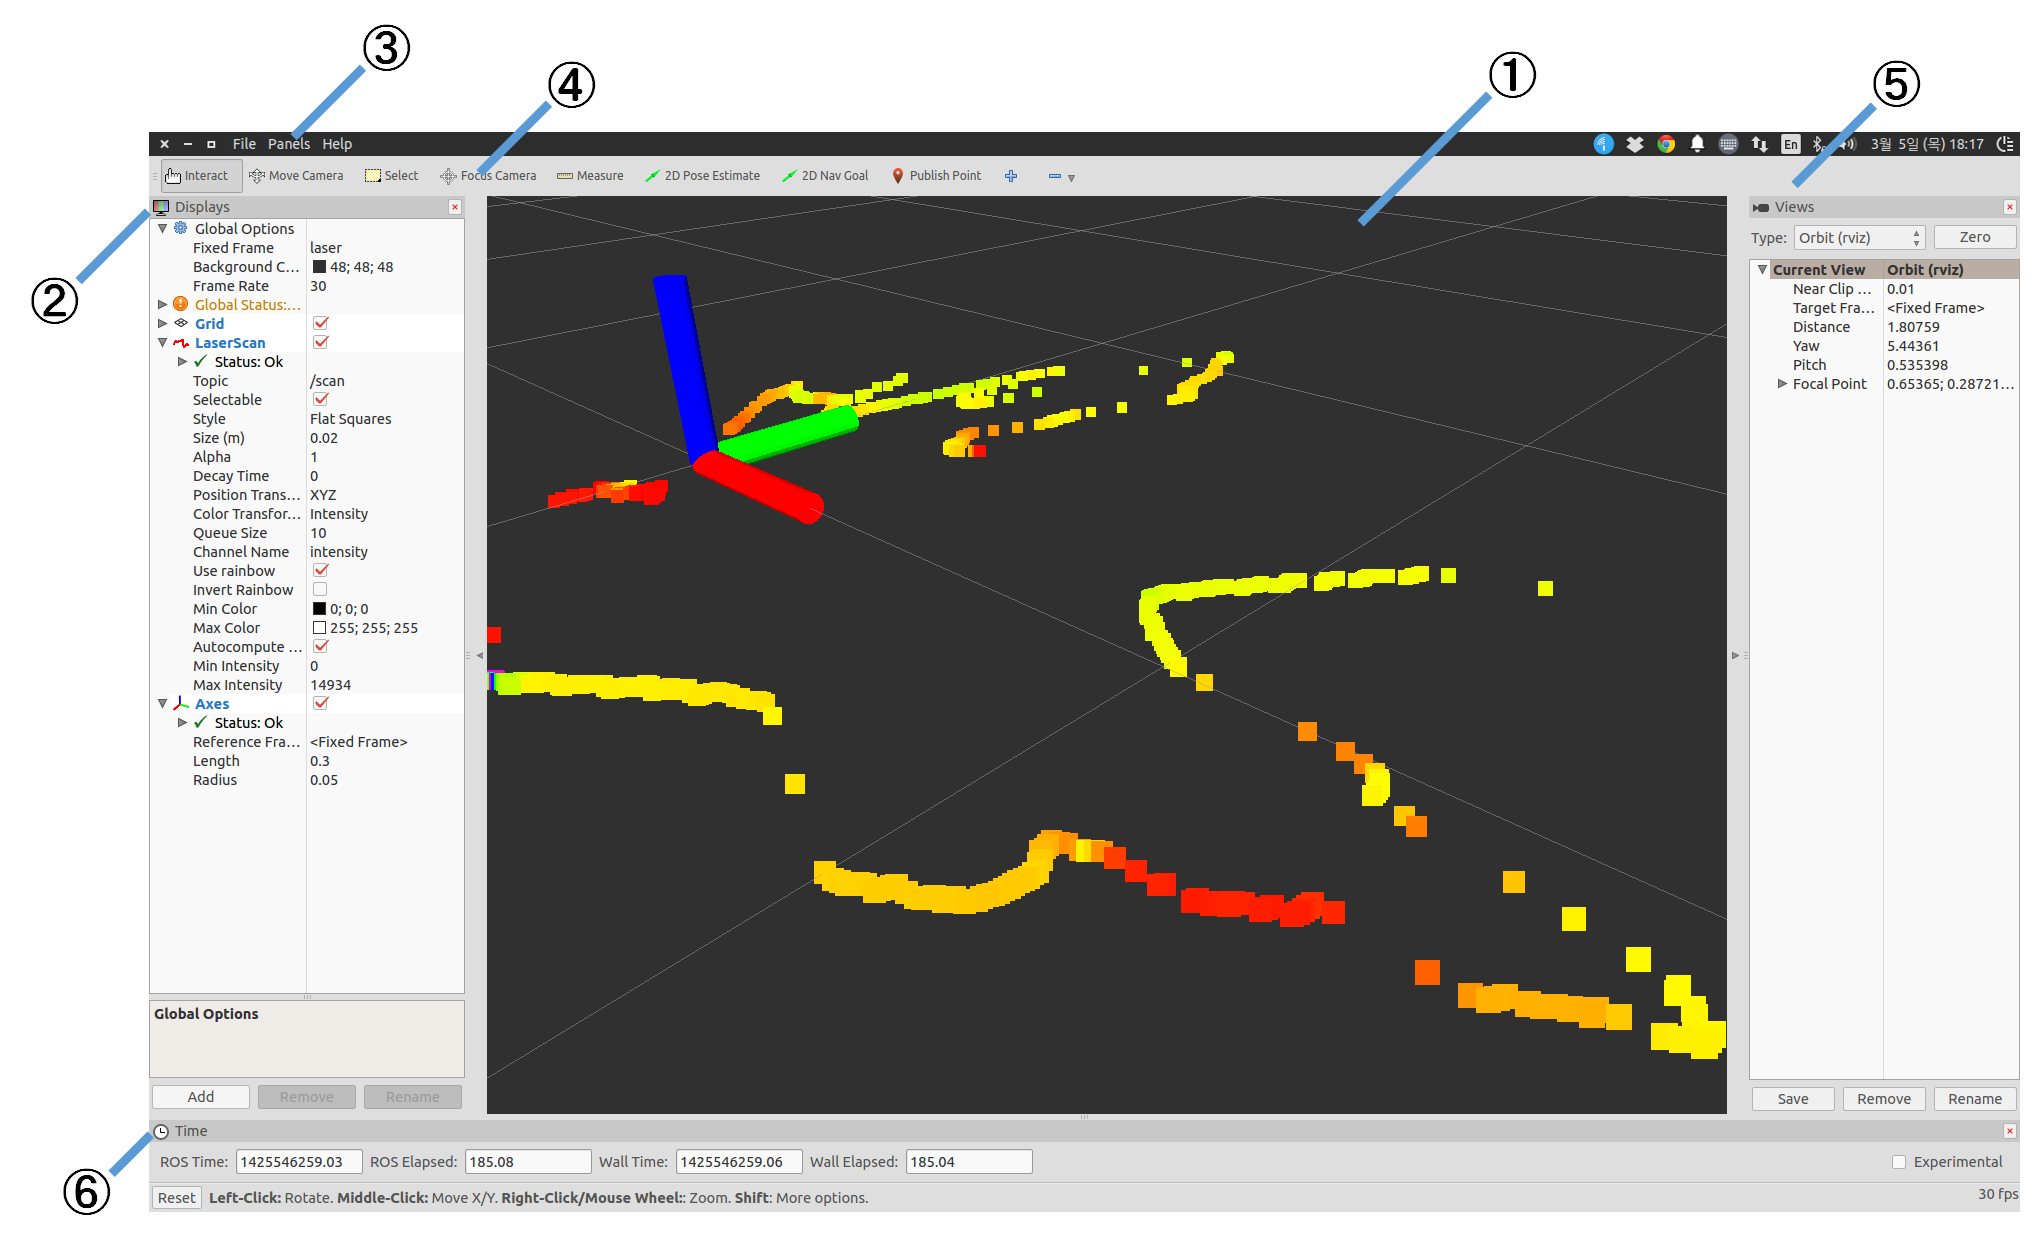
\includegraphics[width=\columnwidth]{pictures/chapter5/pic_05_05.png}
  \caption{RVizの画面構成}
\end{figure}

\begin{itemize}
\item 3Dビュー(3D view):各種データを3次元的に表示するメイン画面である。3Dビューの背景色、固定フレーム、グリッドなどは左側のディスプレイ(Displays)のGlobal OptionsとGrid項目で設定できる。
\item ディスプレイ(Displays):左側にあるディスプレイ設定画面では、様々なトピックに対して、それぞれ適切なデータの表示方法(ディスプレイ)を選択できる。ディスプレイの選択は、画面の左下の<Add>をクリックし、表示された図5-6の選択画面でおこなう。現在、約30種類のディスプレイを選択できる。これについては、後で詳しく説明する。
\itemメニュー(Menu):上部に置かれているメニューでは、現在の表示状態の保存や読み込み、各パネル(3Dビューやディスプレイ、ツールなど)の表示・非表示の切替えができる。
\item ツール(Tools):上部にあるボタンで、カメラの移動、選択、視点方向の変更、距離測定、2次元位置推定、ロボットの移動目標点、パブリッシュポイントなど、様々な機能を実行できる。パブリッシュポイントとは、3Dビュー内をマウスでクリックした点が、/clicked\_pointトピックとして配信される機能である。
\itemビュー(Views):3Dビューの視点を設定する。
  \begin{itemize}
  \item Orbit:特定の3次元位置(注視点)を中心に視点を回転する。(規定値)
  \item FPS(first-person):現在の視点位置を中心に視点を回転する。
  \item TopDownOrtho:XY平面を上からみた視点である。他のビューとは異なり、透視投影法ではなく、平行投影法で表示する。
  \item  XYOrbit:規定値であるOrbitと似ているが、注視点がXY平面上に固定されている。
  \end{itemize}
\item 時間(Time):現在の時間(wall time)とROS Time、またそれぞれの経過時間を示す。経過時間を再起動するには、一番下の<Reset>ボタンをクリックする。
\end{itemize}

\begin{figure}[h]
  \centering
  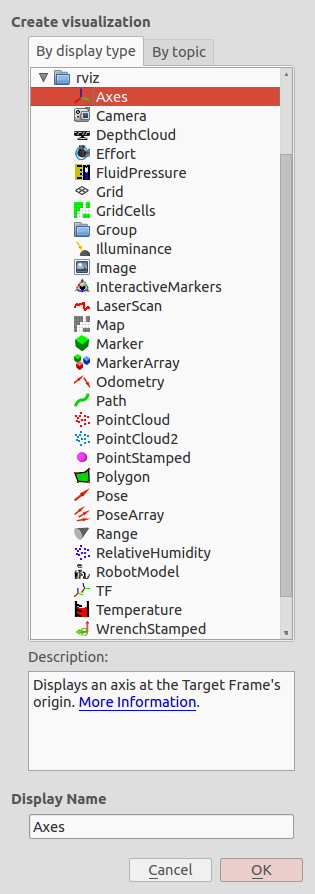
\includegraphics[width=\columnwidth]{pictures/chapter5/pic_05_06.png}
  \caption{RVizディスプレイの選択画面}
\end{figure}

表5-1 Rvizディスプレイ

アイコン  名前  説明

\begin{description}
\item  [Axes]  xyz軸を表示する。
\item  [Camera]  カメラの視点から、新しいレンダリングウィンドウを表示し、その上に画像をオーバーレイする。
\item  [DepthCloud]  奥行き地図(depth map)から得られる点群ポイントクラウド(point cloud)を表示する。主にKinect、Xtionなどのセンサの距離画像(DepthMapトピック)に、カメラ画像(ColorImageトピック)を付加した、色情報の付いた点群データで表示する。
\item  [Effort]  ロボットの各回転関節の力を表示する。
\item  [FluidPressure] 空気、水のような流体の圧力を表示する。
\item  [Grid]  2次元または3次元のグリッドを表示する
\item  [Grid Cells]  グリッドの各セルを表示する。主にナビゲーションのcostmapの障害物表示に使用される。
\item  [Group] ディスプレイをグループ化するコンテナである。ディスプレイを1つのグループとして管理できる。
\item  [Illuminance] 照度を表示する。
\item  [Image] 画像を新しいレンダリングウィンドウに表示する。Cameraディスプレイとは異なり、カメラオーバーレイはしない。
\item  [InteractiveMarkers]  単一または複数のInteractive Markerを表示する。Interactive Markerは、マウスで位置(x、y、z)と姿勢(roll、pitch、yaw)を変えることができる。
\item  [LaserScan] レーザースキャン値を表示する。
\item  [Map] ナビゲーションで使用する占有地図(occupancy map)をground plane上に表示する。
\item  [Marker]  RVizで提供される矢印、円、三角形、長方形、シリンダなどのマーカーを表示する。
\item  [MarkerArray] 上記マーカーを複数表示する。
\item  [Odometry]  時間の経過に伴うオドメトリ(odometry)情報を矢印で表示する。例えば、ロボットが移動すると、通り過ぎたパス上に、矢印マーカーが一定の時間間隔で表示される。
\item  [Path]  ナビゲーションで使用されるロボットの経路を表示する。
\item  [Point Cloud] ポイントクラウド(point cloud)のデータを表示する。Kinect、Xtionなどの3次元計測器から得られる点群データを表示するために使用する。PointCloudとPointCloud2の2種類の形式があり、PointCloud2が最新のPCL(Point Cloud Library) 注1で使用しているフォーマットである。一般的にはPointCloud2を使用すればよい。
\item  [Point Cloud2]
\item  [PointStamped]  丸いポイントを表示する。
\item  [Polygon] ポリゴン(polygon)のアウトラインを表示する。主にロボットの外形などを簡単に2次元上に表現するために使用される。
\item  [Pose]  2次元上のpose(位置と姿勢)を表示する。 Poseを矢印で表現する時、矢印の原点は位置(x、y)を表し、矢印の方向は姿勢(yaw)を示す。ロボットの位置と姿勢や、ナビゲーションの目的点(goal point)にも使用される。
\item  [Pose Array]  上記のposeを複数表示する。
\item  [Range] 超音波や赤外線センサなどの距離センサの測定範囲を円錐形で可視化する。
\item  [RelativeHumidity] 相対湿度を表示する。
\item  [RobotModel]  ロボットモデルを表示する。
\item  [TF]  座標変換値であるtfを表示する。
\item  [Temperature] 温度を表示する。
\item  [WrenchStamped] 「矢印」(力)と「矢印+丸」(トルク)でねじり動作であるレンチ(wrench)を表示する。
\end{description}

%-------------------------------------------------------------------------------
\section{ROS GUI開発ツール rqt}\index{ROS GUI開発ツール rqt}

ROSには、3D視覚化ツールであるRViz以外にも、ロボットの開発に必要な様々なGUIツールがある。例えば、各ノードの階層構造をグラフで示し、現在のノードとトピックの状態を確認できるツールや、トピックのデータを2次元プロットで図示するツールなどである。
ROS Fuerteバージョンから、RVizを含むこれら30種類以上のGUIツールがrqtという名前で統合されて、総合GUIツールとして使用できるようになった。さらに、rqtはその名前が示すようにQtで開発されており、ユーザーが自由にプラグインを開発し追加できる。この節では、rqtのインストール方法から一般的な使い方、さらにrqtのプラグインでも特に使用頻度の高いrqt\_image\_view、rqt\_graph、rqt\_plot、rqt\_bagについて述べていく。

%-------------------------------------------------------------------------------
\subsection{rqtのインストール}

rqtは、ROSを第2章で紹介した方法に従い「sudo apt-get install ros-indigo-desktop-full」でインストールすると、自動的にインストールされる。もし上記以外の方法によりrqtがインストールされていない場合は、次のコマンドでrqtをインストールする。

\vspace{\baselineskip}
\begin{lstlisting}[language=ROS]
$ sudo apt-get install ros-indigo-rqt ros-indigo-rqt-common-plugins
\end{lstlisting}

ただし、rqt\_plotでは、グラフ作成のために追加でインストールしなければならないファイルがある。rqt\_plotはPyQtGraph、MatPlot、QwtPlotをサポートしているが、ここではPyQtGraphを使用する。次のアドレスから最新のpython-pyqtgraph\_0.9.xx-x\_all.debファイルをダウンロードし、インストールする。

http://www.pyqtgraph.org/downloads/

インストールが完了したら、次のコマンドでrqt\_plotを実行する。

\vspace{\baselineskip}
\begin{lstlisting}[language=ROS]
$ rqt_plot
\end{lstlisting}

rqt\_plotを実行し、右上隅にある歯車の形のアイコン(オプションを意味する)をクリックする。表示された図5-7のオプション選択画面で、「Plot Type」の中から「PyQtGraph」を選択する。

\begin{figure}[h]
  \centering
  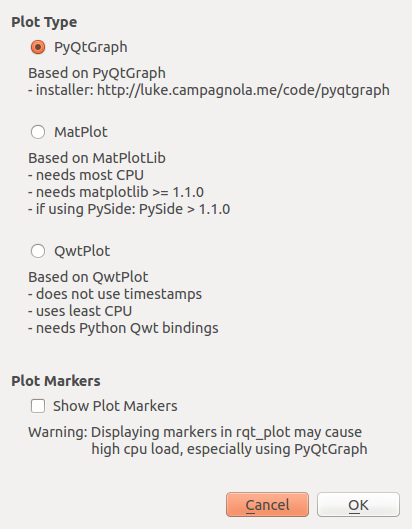
\includegraphics[width=\columnwidth]{pictures/chapter5/pic_05_07.png}
  \caption{rqt\_plotのオプション選択画面}
\end{figure}

%-------------------------------------------------------------------------------
\subsection{rqtの実行とメニュー}

rqtを実行するコマンドは次のとおりである。単にrqtと入力するか、「rosrun rqt\_gui rqt\_gui」と入力する。

\begin{lstlisting}[language=ROS]
$ rqt
\end{lstlisting}

rqtを実行すると、図5-8のようにrqtのgui画面が現れる。初めて起動したときには、メニューのみが表示される。これは、rqt上で実行するプラグインが指定されていないためである。

\begin{figure}[h]
  \centering
  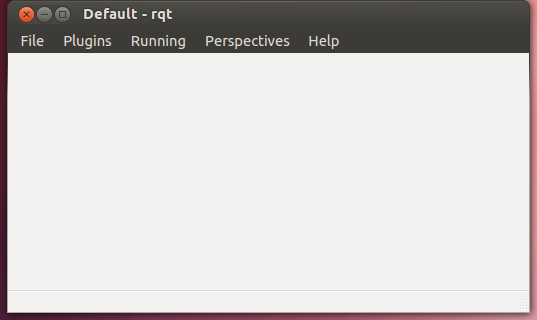
\includegraphics[width=\columnwidth]{pictures/chapter5/pic_05_08.png}
  \caption{rqtの初期画面}
\end{figure}

rqtの各メニューは、次のとおりである。

\begin{itemize}
\item ファイル(File):rqtを終了するサブメニューがある。
\item プラグイン(Plugins):30種類以上のプラグインがある。これらを選択して使用する。
\item 動作(Running):現在動作中のプラグインを表示し、不要なプラグインを停止できる。
\item 画面構成(Perspectives):現在動作中のプラグインを保存し、次回の起動時に同じプラグインを実行できる。
\end{itemize}

%-------------------------------------------------------------------------------
\subsection{rqtプラグイン}

rqtの上部メニューの中から[プラグイン(Plugins)]を選択すると、30種類以上のプラグインが以下の項目に分類されて表示される。ここではrqtの基本的なプラグインを紹介するが、必要なら非公認のrqtプラグインや、ユーザーが開発したrqtプラグインも追加できる。

\textbf{アクション(Action)}
\begin{description}
\item  [Action Type Browser] Actionタイプのデータ構造を確認する。
\end{description}

\textbf{構成(Configuration)}
\begin{description}
\item  [Dynamic Reconfigure] ノードのパラメータ値を変更できる。
\item  [Launch] roslaunchのGUIプラグイン。roslaunchの名前や構成が思い出せないときに便利である。
\end{description}

\textbf{内部構造(Introspection)}
\begin{description}
\item  [Node Graph] 実行されているノードの関係図やメッセージの流れをグラフビュー形式で確認できる。
\item  [Package Graph] パッケージの依存関係をグラフビュー形式で表示する。
\item  [Process Monitor] 現在実行中のノードのPID(プロセッサID)、CPU使用率、メモリ使用率、スレッドの数を確認できる。
\end{description}

\textbf{ロギング(Logging)}
\begin{description}
\item  [Bag] ROSデータロギング関連のプラグイン
\item  [Console] ノードで発生する警告(Warning)、エラー(Error)などのメッセージを一つの画面で確認できる。
\item  [Logger Level] ノードでログ発行を担当するロガーを選択し、ロガーレベルと呼ばれるDebug、Info、Warn、Error、Fatalログ情報を設定するためのプラグイン。デバッグするときDebugを選択して使用すると、非常に便利である。
\end{description}

\textbf{様々なツール(Miscellaneous Tools)}
\begin{description}
\item  [Python Console] Pythonのコンソール画面のプラグイン
\item  [Shell] シェルを駆動する。
\item  [Web] ブラウザを駆動する。
\end{description}

\textbf{ロボット(Robot)}
\begin{itemize}
\item 使用しているロボットに応じて、ダッシュボード(dashboard)などのプラグインをここに追加すればよい。
\end{itemize}

\textbf{ロボットツール(Robot Tools)}
\begin{description}
\item  [Controller Manager] ロボットコントローラの状態、タイプ、ハードウェアインタフェース情報などを確認できる。
\item  [Diagnostic Viewer] ロボット機器およびエラーチェックを行う。
\item  [Moveit!Monitor] モーションプランニングに使用されるMoveIt!データを確認する。
\item  [Robot Steering] ロボットの手動制御GUIツール。遠隔操作では、このGUIツールを利用してロボットを操縦する。
\item  [Runtime Monitor] ノードで発生する警告やエラーを確認できる。
\end{description}

\textbf{サービス(Services)}
\begin{description}
\item  [Service Caller] 起動しているサービスサーバに接続し、サービスリクエストが可能なGUIプラグイン。サービスのテストに適している。
\item  [Service Type Browser] サービスタイプのデータ構造を確認する。
\end{description}

\textbf{トピックス(Topics)}
\begin{description}
\item  [Easy Message Publisher] GUI環境でトピックを発行するプラグインである。現在実行中のノードで使用しているトピックの中から一つのトピックを選択し、メッセージのデータをスライド・バーなどで変更しながらトピックを発行できる。これはトピックのテストに適している。
\item  [Message Publisher] Easy Message Publisherでは、選択した一つのトピックに対してメッセージの変更や配信を行うが、これは全てのトピックに対してメッセージの変更やトピックの配信ができる。トピックの内容は手動で設定する。
\item  [Message Type Browser] トピックのメッセージの型を確認する。
\item  [Topic Monitor] 現在使用しているトピックの一覧を表示し、その中でユーザーが選択したトピックの情報を表示する。
\end{description}

\textbf{可視化(Visualization)}
\begin{description}
\item  [Image View] カメラの映像データを確認できる。
\item  [Navigation Viewer] ナビゲーションで、ロボットの位置や目標地点を確認する。
\item  [Plot] 2次元データのプロットGUIプラグイン。 2次元データの可視化に非常に便利である。
\item  [Pose View] ロボットモデルやtfなどのポーズ(位置と姿勢)を表示する。
\item  [RViz] 3次元可視化ツールであるRVizのプラグイン。rqtでこれを選択すれば、RVizを起動できる。
\item  [TF Tree] tfの関係をツリー構造で表すグラフビュー形式のプラグイン
\end{description}

\begin{figure}[h]
  \centering
  \includegraphics[width=\columnwidth]{pictures/chapter5/pic_05_09.png}
  \caption{rqtプラグイン}
\end{figure}

以降では、最も頻繁に使用されるrqt\_image\_view、rqt\_graph、rqt\_plot、rqt\_bagについて説明する。

%-------------------------------------------------------------------------------
\subsection{rqt\_image\_view}

カメラの画像データを表示するプラグインである。画像処理はできないが、取得映像を確認する用途でよく使われる。一般的なUSBカメラはUVC(USB video device class)をサポートしているので、ROSのuvc\_cameraパッケージを利用すれば簡単に画像を取得できる。まず、次のコマンドでuvc\_cameraパッケージをインストールする。

\begin{lstlisting}[language=ROS]
$ sudo apt-get install ros-indigo-uvc-camera
\end{lstlisting}

USBカメラをコンピュータのUSBに接続して、次のコマンドでuvc\_cameraパッケージのuvc\_camera\_nodeノードを実行する。

\begin{lstlisting}[language=ROS]
$ rosrun uvc_camera uvc_camera_node
\end{lstlisting}

次に「rqt」コマンドでrqtを起動し、メニューから[Plugins]→[Visualization] →[Image View]を選択する。そして、左上のトピック選択ボックスで「/image\_raw」を選択すると、図5-10のようにカメラ映像を確認できる。カメラに関しては8.1節で詳しく説明する。

\begin{lstlisting}[language=ROS]
$ rqt
\end{lstlisting}

\begin{figure}[h]
  \centering
  \includegraphics[width=\columnwidth]{pictures/chapter5/pic_05_10.png}
  \caption{USBカメラの画像データをrqt_image_viewで確認している例}
\end{figure}


%-------------------------------------------------------------------------------
\subsection{rqt\_graph}

rqt\_graphは、実行中のノードとROSネットワーク上で送受信されているメッセージの関係をグラフで表すプラグインである。ROSネットワークの状況を把握するのに非常に便利である。
ここでは、2.5節で説明したturtlesimパッケージのturtlesim\_node、turtle\_teleop\_key、そして前述のuvc\_cameraパッケージのuvc\_camera\_nodeノードを使ってrqt\_graphの使用方法を説明する。まず以下のコマンドで、関連するノードをそれぞれ別のターミナルウィンドウで立ち上げる。

\begin{lstlisting}[language=ROS]
$ rosrun turtlesim turtlesim_node
$ rosrun turtlesim turtle_teleop_key
$ rosrun uvc_camera uvc_camera_node
\end{lstlisting}

その後、次のように、「rqt」コマンドでrqtを実行して、メニューから[Plugins]→[Introspection]→ [Node\_Graph]を選択する。rqt\_graphを実行したときのノードとトピックの関係は、図5-11のように表示される。

\begin{lstlisting}[language=ROS]
$ rqt
\end{lstlisting}

\begin{figure}[h]
  \centering
  \includegraphics[width=\columnwidth]{pictures/chapter5/pic_05_11.png}
  \caption{rqt_graph実行例}
\end{figure}

図5-11で「teleop\_turtle」などの外側の四角は名前空間のグループ(「6.5 roslaunchを用いた複数ノードの起動」を参照)を意味し、その中の「/teleop\_turtle」などの円は、実行した配信者(publisher)や購読者(subscriber)のノードを意味する。「/turtle1/cmd\_vel」と「/image\_raw」を囲む小さな四角はトピックを意味する。矢印は、トピック通信の送受信方向を意味する。図5-11の例では、turtle\_teleop\_key、turtlesim\_nodeを実行すると、teleop\_turtleとturtlesimのノードが立ち上がる。この2つのノードは、キーボードの方向キーが押されたときに配信される「/turtle1/cmd\_vel」トピックを介し、配信者と購読者の間でデータを送受信していることが確認できる。uvc\_cameraパッケージも同様に、配信者であるuvc\_cameraノードが「/imge\_raw」トピックを発行していることが確認できる。
この例ではノードを数個実行しただけであるが、実際のROSプログラミングでは、数十個に及ぶノードが様々なトピックのメッセージを送受信することも珍しくない。このようなとき、rqt\_graphは現在のROSネットワーク上のノードの関係を確認できる、非常に強力なツールである。

%-------------------------------------------------------------------------------
\subsection{rqt\_plot}

rqt\_plotは、ROSメッセージである2次元データを受け取り、2次元座標系上に描画するツールである。例として、turtlesimノードのposeメッセージのxとy座標を描画してみよう。まず、turtlesimパッケージのturtlesim\_nodeを実行する。

\begin{lstlisting}[language=ROS]
$ rosrun turtlesim turtlesim_node
\end{lstlisting}

そして、次の例のようにrqtを実行した後、メニューから[Plugins]→[Visualization]→[Plot]を選択すると、rqt\_plotが実行される。 rqt\_plot上部のTopic欄に「/turtle1/pose」と入力すれば、「/turtle1/pose」トピックが2次元(x軸:データの値、y軸:時間)の上に図式化される。

\begin{lstlisting}[language=ROS]
$ rqt
\end{lstlisting}

あるいは、次のコマンドのように、トピックを指定して実行することもできる。

\begin{lstlisting}[language=ROS]
$ rqt_plot /turtle1/pose/
\end{lstlisting}

次に、turtlesimパッケージのturtle\_teleop\_keyを実行して、画面の中の亀を前後に動かしてみよう。

\begin{lstlisting}[language=ROS]
$ rosrun turtlesim turtle_teleop_key
\end{lstlisting}

その結果、図5-12のように亀の位置、姿勢、そして速度と角速度が表示されることが確認できる。
このようにrqt\_plotは2次元データの表示に便利なツールである。今回はturtlesimに対して利用したが、ユーザーが開発したノードの2次元データの表示にも利用できる。特に、速度や加速度などの時間経過を伴うセンサの値を表示するのに適している。

\begin{figure}[h]
  \centering
  \includegraphics[width=\columnwidth]{pictures/chapter5/pic_05_12.png}
  \caption{rqt\_plotの使用例}
\end{figure}

%-------------------------------------------------------------------------------
\subsection{rqt\_bag}

rqt\_bagはbagファイルに保存したメッセージを視覚化するGUIツールである。4.4.8項で取り上げたrosbagはテキストベースであるが、rqt\_bagはこれに可視化機能が追加されたものであり、カメラ画像なども確認できる。これをテストする前に、rqt\_image\_viewと、rqt\_graphツールの説明で用いたturtlesimとuvc\_camera関連ノードをすべて実行する。次に、以下のコマンドで、uvc\_cameraの「/image\_raw」トピックとturtlesimの「/turtle1/cmd\_vel」トピックをbagファイルに保存する。

\begin{lstlisting}[language=ROS]
$ rosrun uvc_camera uvc_camera_node
$ rosbag record /image_raw
$ rqt
\end{lstlisting}

rqt\_bagは、rosbagと同様に、トピックメッセージの保存、再生、圧縮などが可能である。加えて、GUIプログラムで構成されており、すべてのコマンドはボタンで動作する。このため、操作が容易で、カメラの映像をビデオ編集プログラムのように時間軸を合わせながら確認できる。実際に、USBカメラの映像をbagファイルとして保存した後、rqt\_bagで再生してみよう。
「rqt」コマンドでrqtを実行し、メニューの[Plugins]→[Logging]→[Bag]を選択する。次に、左上のフォルダの形(Load Bag)のアイコンを選択して、上の「rosbag record /image\_raw」コマンドで記録した「*.bag」ファイルを開く。これにより、図5-13のようにカメラの映像を時間軸の変化とともに確認できる。また、このツールは映像の拡大、一定時間のデータ数の確認などができ、さらにマウスの右ボタンを押した後、「Publish」オプションをクリックすると、メッセージの再発行も可能である。

\begin{figure}[h]
  \centering
  \includegraphics[width=\columnwidth]{pictures/chapter5/pic_05_13.png}
  \caption{rqt\_bagの使用例}
\end{figure}

以上でrqtツールのインストール、使用方法について概略を説明した。この節では、すべてのプラグインについては説明できなかったが、ここで示したいくつかの例を参考に、様々なオプション機能を試してほしい。rqtツールは、他のROSノードのようにロボットやセンサを直接処理するものではないが、開発作業を行う上で、データの保存、修正、分析、デバッグなどに役立つ便利な補助ツールである。

% 注1  http://pointclouds.org/

% !TEX root = ./rosbook_jp.tex
%-------------------------------------------------------------------------------
\chapterimage{chapter_head_6.pdf}

%-------------------------------------------------------------------------------
\chapter{ROSプログラミングの基本}

%-------------------------------------------------------------------------------
\section{メッセージ、トピック、サービス、パラメータ}
\index{メッセージ}\index{トピック}\index{サービス}\index{パラメータ}\index{Message}\index{Topic}\index{Service}\index{Parameter}

5章まではROSの概要や、コマンド、ツールなどを紹介した。本章からは本格的にROSプログラミングについて説明していく。
ここまでで最も頻繁に使われた用語は、メッセージ、トピック、サービス、パラメータなどである。ROSプログラミングにおける最小の実行単位であるノードは、メッセージ通信を介してほかのノードとデータをやり取りするが、それに使用される方式がトピック、サービスである。一方、パラメータ通信は、パラメータサーバとノード間でパラメータ値をやり取りする際に用いられる。本節では、メッセージ通信、パラメータ通信の概念、および具体的な通信方式を、実例を交えて説明する。

\begin{definition*}[ROSで使用される通信]
ROSで使用される通信には、ノード間でメッセージをやり取りするメッセージ通信と、パラメータサーバとノード間でパラメータ値をやり取りするパラメータ通信    がある。図6-1にメッセージ通信とパラメータ通信の概要を示す 。メッセージ通信は、一方向通信方式のトピック(topic)通信と、双方向通信方式のサービス(service)通信に分けることができる。
\end{definition*}

\begin{figure}[h]
  \centering
  \includegraphics[width=10cm]{pictures/chapter6/pic_06_01.png}
  \caption{ノード間のメッセージ通信とパラメータ通信}
\end{figure}

\begin{definition*}[トピック(topic)通信]
トピック通信とは、ノードからノードへ一方向にメッセージを送信する手段である。この時、メッセージを配信するノードを配信者(publisher)ノード、購読するノードを購読者(subscriber)ノードという。配信者ノードはメッセージを配信する際に、マスターにトピック名を登録する。トピック(話題)とはメッセージの内容を表すラベルである。トピックの購読を購読者ノードが希望すると、マスターはそのトピックを配信している配信者ノードの情報を購読者ノードに伝える。この情報をもとに、購読者ノードと配信者ノードは直接通信を行う。
トピック通信は一方向通信であるが、一回接続された配信者ノードと購読者ノードは、その後は連続して通信を行うことができるという特徴をもつ。そのため、センサからセンサドライバを通して直接計測値を読み込むノードを配信者ノード、計測値を加工してより高度な情報処理を行うノードを購読者ノードとするなど、連続してメッセージを送る必要があるセンサデータ送信に適している。
\end{definition*}

\begin{figure}[h]
  \centering
  \includegraphics[width=10cm]{pictures/chapter6/pic_06_02.png}
  \caption{トピック通信}
\end{figure}

\begin{definition*}[サービス(service)通信]
サービス通信   とは、ノード間でリクエスト/レスポンス方式でメッセージをやり取りする手段である。リクエストを送り、レスポンスを待つノードをサービスクライアント(service client)、リクエストを受けた後、レスポンスを返すノードをサービスサーバ(service server)という。サービスサーバは起動と同時に、マスターにサービス名を登録する。サービスクライアントがサービスリクエストを送る際、マスターはそのサービスサーバの情報をサービスクライアントに伝える。その後、サービスクライアントはサービスサーバと直接接続し、サービス通信を行う。
サ  ービスは、トピックとは異なり、一回限りのメッセージ通信であるため、サービスのリクエストとレスポンスが完了すると、2つのノードの接続は切断される。  サービス通信は、ロボットへの定型動作の実行命令や、特定の条件が満たされたときにイベントを発生するノードなどに使用される。
\end{definition*}

\begin{figure}[h]
  \centering
  \includegraphics[width=10cm]{pictures/chapter6/pic_06_03.png}
  \caption{サービス通信}
\end{figure}

\begin{definition*}[パラメータ(parameter)通信]
パラメータ通信とは、ノードのパラメータを設定する、パラメータサーバとノード間の通信である。パラメータサーバはROSネットワーク内に1つだけ存在し、ROSマスターの起動と同時に自動的に立ち上がる。  ノードの動作開始時に、各ノードはパラメータのパラメータ名とその規定値をパラメータサーバに書き込む。  その後、rosparamコマンドなどでユーザがパラメータサーバに登録されているパラメータ値を書き換えると、各ノードはパラメータ通信によりパラメータサーバのパラメータ値を読み込み、ノードのパラメータを変更する。これにより、ノードの動作開始後に、ノードの動作を変更することができる。
パラメータ通信はトピック通信やサービス通信とは異なり、ノード間通信に用いるものではなく、ノードとパラメータサーバ間の通信に使われる。具体的には、  デバイスポートの指定、センサ計測範囲の設定などに利用される。
\end{definition*}

\begin{figure}[h]
  \centering
  \includegraphics[width=10cm]{pictures/chapter6/pic_06_04.png}
  \caption{パラメータ通信}
\end{figure}

%-------------------------------------------------------------------------------
\section{トピック通信の実践}
\index{トピック}\index{Topic}

トピック  通信では、送信側のノードを「Publisher(配信者)」、受信側のノードを「Subscriber(購読者)」と呼ぶ。本節では、メッセージファイルと配信者ノード、購読者ノードを含む簡単なパッケージを作成する  ことで、ROSにおけるトピックを用いた通信方式を理解する。

%-------------------------------------------------------------------------------
\subsection{パッケージの作成}

まず、irvs\_ros\_tutorialsという名前のパッケージを作成する。このパッケージでは、ROSの標準的なメッセージパッケージのstd\_msgsと、ROSでC/C++を使用する際に必要なクライアントライブラリroscppを使用する。このため、これをオプションで指定してcatkin\_create\_pkgを実行する。

\begin{lstlisting}[language=ROS]
$ cd ~/catkin_ws/src
$ catkin_create_pkg irvs_ros_tutorials std_msgs roscpp
\end{lstlisting}

std\_msgsやroscppなどのパッケージは、作成されたパッケージをビルドする前に、あらかじめインストールしておく必要がある。これら依存するパッケージやライブラリの設定は、上記のようにcatkin\_create\_pkgコマンドで新たにパッケージを作成するときに指定することもできるが、  作成した後にpackage.xmlを直接編集して指定することもできる。

パッケージを作成すると、「\verb|~|/catkin\_ws/src」フォルダにirvs\_ros\_tutorialsパッケージフォルダが作られ、その中に必要なROSのパッケージやCMakeLists.txt、 package.xmlファイルが置かれる。次のようにlsコマンドを入力するか、Nautilusを利用してパッケージのフォルダを確認すると、以下のように表示される。次項では、ここで作成されたpackage.xml、CMakeLists.txtを修正する。

\begin{lstlisting}[language=ROS]
$ cd irvs_ros_tutorials
$ ls
include     %*→ヘッダーファイルフォルダ*)
src     %*→ソースコードフォルダ*)
CMakeLists.txt    %*→ビルド設定ファイル*)
package.xml   %*→パッケージの設定ファイル*)
\end{lstlisting}

%-------------------------------------------------------------------------------
\subsection{パッケージの設定ファイル(package.xml)の修正}

ROSの必須の設定ファイルであるpackage.xmlは、パッケージ名、著作者、ライセンス、依存パッケージなどのパッケージの情報をXML形式で記述している。gedit、vim、emacsなどの文書編集プログラムでこのファイルを開き、現在のノードに合わせて内容を変更する。つぎのコマンドはUbuntu標準の文書編集プログラムgeditでpackage.xmlファイルを編集する例である。

\begin{lstlisting}[language=ROS]
$ gedit package.xml
\end{lstlisting}

以下のpackage.xmlファイルは、6.2.1項で作成したファイルを本節で作成するパッケージ  に合わせて変更した例である。  各オプションの詳細については、3.4.2項を参照してほしい。

\noindent\textbf{ファイル名: package.xml}
\begin{lstlisting}[language=XML]
<? xml version = "1.0" ?>
<package>
<name>irvs_ros_tutorials</name>
<version> 0.1.0 </version>
<description>The irvs_ros_tutorials package</description>
<maintainer email = "aaa@bbb.jp">Anonymous</maintainer>
<url type = "website"> http://irvs.github.io/ros_tms/</url>
<url type = "repository"> https://github.com/irvs/irvs_ros_tutorials.git </url>
<author email = "aaa@bbb.jp">Anonymous</author>

<license> BSD </license>

<buildtool_depend> catkin </buildtool_depend>

<build_depend> roscpp </build_depend>
<build_depend> std_msgs </build_depend>
<build_depend> message_generation </build_depend>

<run_depend> roscpp </run_depend>
<run_depend> std_msgs </run_depend>
<run_depend> message_runtime </run_depend>

<export>
</export>
</package>
\end{lstlisting}

%-------------------------------------------------------------------------------
\subsection{ビルド設定ファイル(CMakeLists.txt)の修正}

続いて同じフォルダのCMakeLists.txtファイルに、実行ファイルの作成、依存パッケージの優先ビルド、リンクの作成などを設定する。

\begin{lstlisting}[language=ROS]
$ gedit CMakeLists.txt
\end{lstlisting}

以下のCMakeLists.txtは、6.2.1項で作成したファイルを本節で作成するパッケージに合わせて変更したものである。前項のpackage.xmlファイルと同様に、各オプションの詳細については3.4.3項を参照してほしい。

\noindent\textbf{ファイル名: CMakeLists.txt}
\begin{lstlisting}[language=make]
cmake_minimum_required (VERSION 2.8.3)
project(irvs_ros_tutorials)

## %*catkinビルドに必要なコンポーネントパッケージの設定*)
## %*これらのパッケージが存在しない場合、catkinビルドの途中でエラーが出る。*)
find_package(catkin REQUIRED COMPONENTS roscpp std_msgs message_generation)

## %*メッセージファイルの設定*)
add_message_files(FILES msgTutorial.msg)

##  %*add\_message\_filesで使用するメッセージの依存関係を設定*)
## %*これらのパッケージが存在しない場合、catkinビルドの途中でエラーが出る。*)
generate_messages(DEPENDENCIES std_msgs)

## %*インクルードディレクトリ、ライブラリ、catkinビルド、システムに依存するパッケージの指定*)
catkin_package(
  INCLUDE_DIRS include
  LIBRARIES irvs_ros_tutorials
  CATKIN_DEPENDS roscpp std_msgs
  DEPENDS system_lib
)

## %*インクルードディレクトリの設定*)
include_directories(include ${catkin_INCLUDE_DIRS})

## %*ros\_tutorial\_msg\_publisherノードの設定*)
## %*実行ファイル、ターゲットリンクライブラリ、追加の依存関係などを設定*)
add_executable(ros_tutorial_msg_publisher
  src/ros_tutorial_msg_publisher.cpp)
target_link_libraries(ros_tutorial_msg_publisher ${catkin_LIBRARIES})
add_dependencies(ros_tutorial_msg_publisher
  irvs_ros_tutorials_generate_messages_cpp)

## %*ros\_tutorial\_msg\_subscriberノードの設定*)
## %*実行ファイル、ターゲットリンクライブラリ、追加の依存関係などを設定*)
add_executable(ros_tutorial_msg_subscriber
  src/ros_tutorial_msg_subscriber.cpp)
target_link_libraries(ros_tutorial_msg_subscriber ${catkin_LIBRARIES})
add_dependencies(ros_tutorial_msg_subscriber
  irvs_ros_tutorials_generate_messages_cpp)
\end{lstlisting}

%-------------------------------------------------------------------------------
\subsection{メッセージファイルの作成}
\index{メッセージファイル}\index{msg}

前項でCMakeLists.txtファイルには、次のようなオプションを追加した。

\begin{lstlisting}[language=make]
add_message_files(FILES msgTutorial.msg)
\end{lstlisting}

このオプションは、6.2.1項で作成したパッケージに含まれるノードでmsgTutorial.ms\\gメッセージを使用するため、そのメッセージ型を定義したmsgTutorial.hファイルを作成する ための設定である。ただしメッセージファイルmsgTutorial.msg自体はまだ作成していないので、次の手順で作成する。

\begin{lstlisting}[language=ROS]
$ roscd irvs_ros_tutorials  %*→パッケージフォルダに移動*)
$ mkdir msg    %* →パッケージにmsgフォルダを新規作成*)
$ cd msg      %*→作成したmsgフォルダに移動*)
$ gedit msgTutorial.msg %*→msgTutorial.msgファイルを新規作成する*)
\end{lstlisting}

メッセージ内容は以下の通りで、int32(32ビット整数型)メッセージ形式のdata変数を宣言している  。

\begin{lstlisting}[language=ROS]
int32 data
\end{lstlisting}

メッセージタイプはint32以外にもbool、int8、int16、float32、string、time、durationなどの基本的な形式   、およびactionlib\_msgsやdiagnostic\_msgsなど、ROSで多く使用されているメッセージをまとめたcommon\_msgsなどがある。ここでは、最も簡単な例としてint32を宣言した。

\begin{exercise}[メッセージ・サービスファイルの独立パッケージ化]
メッセージファイルmsgとサービスファイルsrvは、実行ノードパッケージに含めるのではなく、メッセージファイルだけで構成された独立したパッケージとすることを推奨する。購読者ノードと配信者ノードを別のコンピュータ上で実行するとき、その両方のノードには相互に依存関係があるので、片方のノードにしか関連しないパッケージやノードであっても、すべて双方のコンピュータに  インストールする必要がある。しかしメッセージのみの独立したパッケージを個別に作成しておけば、このパッケージのみを追加でインストールすればよく    、一方のノードだけに関連したパッケージを他方のノードを実行するコンピュータにインストールする必要がなくなる。ただし、本書では、コードを簡潔に示すため、メッセージファイルを実行ノードパッケージに含めている。
\end{exercise}

%-------------------------------------------------------------------------------
\subsection{配信者ノードの作成}
\index{配信者}\index{Publisher}

前述のCMakeLists.txtファイルには、次のような配信者  ノードの実行ファイルを生成するオプションを追加した。

\begin{lstlisting}[language=make]
add_executable(ros_tutorial_msg_publisher  src/ros_tutorial_msg_publisher.cpp)
\end{lstlisting}

これは、srcフォルダのros\_tutorial\_msg\_publisher.cppという名前のファイルから、ros\_tutorial\_msg\_publisherという実行ファイルを作成することを意味する。次の手順で配信者ノードのためのプログラムを作成してみよう。

\begin{lstlisting}[language=ROS]
$ roscd irvs_ros_tutorials/src %*→ パッケージのソースフォルダであるsrcフォルダに移動*)
$ gedit ros_tutorial_msg_publisher.cpp %*→ ソースファイルの新規作成と内容の変更*)
\end{lstlisting}

\noindent\textbf{ファイル名: ros\_tutorial\_msg\_publisher.cpp}
\begin{lstlisting}[language=C++]
// %*ROSメインヘッダーファイル*)
// %*ROSプログラミングを行う際に必要となるROSファイルのインクルードを行う。*)
// %*後述するROS\_INFO関数などを使用できるようになる。*)
#include "ros/ros.h"

// %*msgTutorialメッセージファイルのヘッダー*)
// %*CMakelists.txtでビルド後に自動的に生成されるように設定した*)
// %*メッセージファイルのヘッダーをインクルードする。*)
#include "irvs_ros_tutorials/msgTutorial.h"

// %*配信者ノードのメイン関数*)
int main(int argc, char **argv)
{
  // %*ノード名の初期化*)
  ros::init(argc, argv, "ros_tutorial_msg_publisher");
  // %*ROSシステムとの通信のためのノードハンドルを宣言*)
  ros::NodeHandle nh;

  // %*配信者ノードの宣言*)
  // %*irvs\_ros\_tutorialsパッケージのmsgTutorialメッセージファイルを*)
  // %*利用した配信者ros\_tutorial\_pubを宣言する。*)
  // %*トピック名を ros\_tutorial\_msg とし、配信者キュー( queue )の*)
  // %*サイズを100に設定する。*)
  // %*配信者キューには、メッセージを送る際、メッセージデータを蓄積する。*)
   // %*http://wiki.ros.org/msg*)
   ros::Publisher ros_tutorial_pub =
     nh.advertise<irvs_ros_tutorials::msgTutorial>("ros_tutorial_msg", 100);

   // %*ループの周期を設定する。 "10"は10Hzを表し、0.1秒間隔で繰り返される*)
   // %*http://wiki.ros.org/roscpp/Overview/Time*)
  ros::Rate loop_rate(10);

  // %*メッセージに使用する変数の宣言*)
  int count = 0;

  // %*ros::ok()はROSの動作が正常であるならtrueを返す関数である。*)
  while (ros::ok())
  {
    // %*msgTutorialメッセージファイル形式でmsg変数を宣言する。*)
    irvs_ros_tutorials::msgTutorial msg;

    // %*変数countを使用して、メッセージの値を定める。*)
    msg.data = count;

    // %*ROS\_INFOというROS関数を使用して、count変数を表示する。*)
    ROS_INFO("send msg = %d", count);

    // %*メッセージを発行する。約0.1秒間隔で発行される。*)
    ros_tutorial_pub.publish(msg);

    // %*上で定められたループサイクルになるように、スリープに入る*)
    loop_rate.sleep();

    // %*count変数に1ずつ増加*)
    ++count;
  }
  return 0;
}
\end{lstlisting}

%-------------------------------------------------------------------------------
\subsection{購読者ノードの作成}
\index{購読者}\index{Subscriber}
CMakeLists.txtファイルには、次のような購読者 ノードの実行ファイルを生成するオプションを追加した。

\begin{lstlisting}[language=make]
add_executable(ros_tutorial_msg_subscriber src/ros_tutorial_msg_subscriber.cpp)
\end{lstlisting}

これは、srcフォルダのros\_tutorial\_msg\_subscriber.cppという名前のファイルから、ros\_tutorial\_msg\_subscriberという実行ファイルを作成することを意味する。次の手順で購読者ノードのためのプログラムを作成してみよう。

\begin{lstlisting}[language=ROS]
$ roscd irvs_ros_tutorials/src %*→ パッケージのソースフォルダであるsrcフォルダに移動*)
$ gedit ros_tutorial_msg_subscriber.cpp %*→ ソースファイルの新規作成と内容の変更*)
\end{lstlisting}

\noindent\textbf{ファイル名: ros\_tutorial\_msg\_subscriber.cpp}
\begin{lstlisting}[language=C++]
// %*ROSメインヘッダーファイル*)
// %*ROSプログラミングを行う際に必要となるROSファイルのインクルードを行う。*)
// %*後述するROS\_INFO関数などを使用できるようになる。*)
#include "ros/ros.h"

// %*msgTutorialメッセージファイルのヘッダー*)
// %*CMakelists.txtでビルド後に自動的に生成されるように設定した*)
// %*メッセージファ//イルのヘッダーをインクルードする。*)
#include "irvs_ros_tutorials/msgTutorial.h"

// %*メッセージを受信したときに動作するコールバック関数を定義*)
// %*irvs\_ros\_tutorialsパッケージのmsgTutorialメッセージを受信する*)
void msgCallback(const irvs_ros_tutorials::msgTutorial::ConstPtr& msg)
{
  // %*受信したメッセージを表示する。*)
  ROS_INFO("recieve msg: %d", msg->data);
}

// %*購読者ノードのメイン関数*)
int main(int argc, char **argv)
{
  // %*ノード名の初期化*)
  ros::init(argc, argv, "ros_tutorial_msg_subscriber");
  // %*ROSシステムとの通信のためのノードのハンドルを宣言*)
  ros::NodeHandle nh;

  // %*購読者ノードの宣言*)
  // %*irvs\_ros\_tutorialsパッケージのmsgTutorialメッセージファイルを*)
  // %*利用した購読者ros\_tutorial\_subを宣言する。*)
  // %*トピック名をros\_tutorial\_msg とし、購読者キュー( queue )の*)
  // %*サイズを100に設定する。*)
  // %*購読者キューには、配信者から送信されてくるメッセージが蓄積される。*)
  ros::Subscriber ros_tutorial_sub = nh.subscribe("ros_tutorial_msg",
   100, msgCallback);

  // %*メッセージが受信されるまで待機し、受信が行われた場合、*)
  // %*コールバック関数を実行する。*)
  ros::spin();

  return 0;
}
\end{lstlisting}

%-------------------------------------------------------------------------------
\subsection{ROSノードのビルド}

次のコマンドでirvs\_ros\_tutorialsパッケージのメッセージファイル、配信者ノード、購読者ノードをビルドする。

\begin{lstlisting}[language=ROS]
$ cd ~/catkin_ws  %*→ catkinフォルダに移動*)
$ catkin_make   %*→ catkinビルドを実行する*)
\end{lstlisting}

irvs\_ros\_tutorialsパッケージのプログラムは、「\verb|~|/catkin\_ws/src/irvs\_ros\_tutorials/src」フォルダにあり、irvs\_ros\_tutorialsパッケージのメッセージファイルは「\verb|~|/catkin\_ws/src\\/irvs\_ros\_tutorials/msg」フォルダにある。
このコマンドにより、「\verb|~|/catkin\_ws/build」と「\verb|~|/catkin\_ws /develフォルダにそれぞれファイルが生成される。「\verb|~|/catkin\_ws/build」フォルダには、catkinビルドで使用された設定内容が保存され、「\verb|~|/catkin\_ws/devel/lib/irvs\\\_ros\_tutorials」フォルダには実行ファイルが、「\verb|~|/catkin\_ws/devel/include/irvs\_ros\_tutorials\\」にはメッセージファイルから自動生成されたヘッダーファイルが保存される。

%-------------------------------------------------------------------------------
\subsection{配信者ノードの実行}

それでは、作成した配信者ノードを実行しよう。ノードの実行前にroscoreを実行して、マスターを起動する。

\begin{lstlisting}[language=ROS]
$ roscore
\end{lstlisting}

その後、別のターミナルウインドウを開き、ROSのノード実行コマンドであるrosrunを利用して、irvs\_ros\_tutorialsパッケージのros\_tutorial\_msg\_publisherノードを起動する。

\begin{lstlisting}[language=ROS]
$ rosrun irvs_ros_tutorials ros_tutorial_msg_publisher
\end{lstlisting}

配信者ノードを実行すると、図6-5のような出力画面が表示され、ROSメッセージが配信されているのがわかる。

\begin{figure}[h]
  \centering
  \includegraphics[width=10cm]{pictures/chapter6/pic_06_05.png}
  \caption{ros\_tutorial\_msg\_publisherノードの実行画面}
\end{figure}

4章で紹介したrostopicコマンドを実行して、ROSのネットワークで使用されているトピックのリストを確認してみよう。rostopicコマンドにlistオプションを付けて実行すると、ros\_tutorial\_msgトピックがあることを確認できる。

\begin{lstlisting}[language=ROS]
$ rostopic list
/ros_tutorial_msg
/rosout
/rosout_agg
\end{lstlisting}

次に、rostopicコマンドにechoオプションを付けて、ros\_tutorial\_msgトピックのメッセージの内容を表示すると、図6-6のように「data: 2」などの実際に配信されているトピックの内容が確認できる  。

\begin{lstlisting}[language=ROS]
$ rostopic echo /ros_tutorial_msg
\end{lstlisting}

\begin{figure}[h]
  \centering
  \includegraphics[width=10cm]{pictures/chapter6/pic_06_06.png}
  \caption{ros\_tutorial\_msgトピックの内容}
\end{figure}

%-------------------------------------------------------------------------------
\subsection{購読者ノードの実行}

配信者ノードを実行したまま、購読者ノードを実行する。新しいターミナルウインドウを開き、ROSのノード実行コマンドであるrosrunを利用して、irvs\_ros\_tutorialsパッケージのros\_tutorial\_msg\_subscriberノードを起動する。

\begin{lstlisting}[language=ROS]
$ rosrun irvs_ros_tutorials ros_tutorial_msg_subscriber
\end{lstlisting}

購読者ノードを実行すると、図6-7のような出力画面が表示される。配信者ノードから送信されたros\_tutorial\_msgトピックのメッセージを、購読者ノードが受信した結果が表示される。

\begin{figure}[h]
  \centering
  \includegraphics[width=10cm]{pictures/chapter6/pic_06_07.png}
  \caption{ros\_tutorial\_msg\_subscriberノードの実行画面}
\end{figure}


%-------------------------------------------------------------------------------
\subsection{実行ノードの通信状態の確認}

配信者および購読者ノードを実行したら、5.2節で紹介したrqtを利用して、実行中のノードの通信状態を確認してみよう。次のようにrqt\_graph、あるいはrqtのいずれかを実行する。

\begin{lstlisting}[language=ROS]
$ rqt_graph
\end{lstlisting}

\begin{lstlisting}[language=ROS]
$ rqt
\end{lstlisting}

rqt上のメニューの[Plugins]→[Introspection]→[Node Graph]を選択すれば、図6-8のように、現在ROSで実行しているノードとメッセージが確認できる。

\begin{figure}[h]
  \centering
  \includegraphics[width=10cm]{pictures/chapter6/pic_06_08.png}
  \caption{ノードの関係をrqt上で表示した結果}
\end{figure}

図6-8では、現在のROSネットワーク上には、配信者ノード(ros\_tutorial\_msg\_publish\\er)がトピック(ros\_tutorial\_msg)を配信しており、これを購読者ノード(ros\_tutorial\_msg\_\\subscriber)が受信していることが確認できる。

%-------------------------------------------------------------------------------
\section{サービス通信の実践}
\index{サービス}\index{Service}

本節では、単純なサービス·ファイルとサービスサーバ(server)ノード、サービスクライアント(client)ノードを作成する。前節で既にirvs\_ros\_tutorialsという名前のパッケージを作成したので、これを利用する。6.2.1項で行ったpackage.xmlファイルの修正は、ここでは必要ないので省略する。

%-------------------------------------------------------------------------------
\subsection{ビルド設定ファイル(CMakeLists.txt)の修正}

前節で作成したirvs\_ros\_tutorialsパッケージに、新しいサービスサーバノード、クライアントノード、サービスファイル(*.srv)を追加する。まず、次のようにirvs\_ros\_tutorial\\sパッケージに移動した後、CMakeLists.txtファイルを変更する。

\begin{lstlisting}[language=ROS]
$ roscd irvs_ros_tutorials
$ gedit CMakeLists.txt
\end{lstlisting}

以下のCMakeLists.txtは、6.2.3項で作成したファイルを本節で作成するパッケージに合わせて変更したものである。前節のパッケージに、サービスサーバノードとクライアントノード、サービスファイル(*.srv)の内容を追加した(太字)。各オプションの詳細については、3.4.3項を参照してほしい。

\noindent\textbf{ファイル名: CMakeLists.txt}
\begin{lstlisting}[language=make]
cmake_minimum_required(VERSION 2.8.3)
project(irvs_ros_tutorials)

## %*catkinビルドに必要なコンポーネントパッケージの設定*)
## %*これらのパッケージが存在しない場合、catkinビルドの途中でエラーが出る。*)
find_package(catkin REQUIRED COMPONENTS roscpp std_msgs message_generation)

## %*メッセージファイルの設定*)
add_message_files(FILES msgTutorial.msg)

## %*サービスファイルの設定*)
add_service_files(FILES srvTutorial.srv)

## %*add\_message\_filesで使用するメッセージの依存関係を設定*)
## %*これらのパッケージが存在しない場合、catkinビルドの途中でエラーが出る。*)
generate_messages(DEPENDENCIES std_msgs)

## %*インクルードディレクトリ、ライブラリ、catkinビルド、システムに依存するパッケージの指定*)
catkin_package(
  INCLUDE_DIRS include
  LIBRARIES irvs_ros_tutorials
  CATKIN_DEPENDS roscpp std_msgs
  DEPENDS system_lib
)

## %*インクルードディレクトリの設定*)
include_directories(include ${catkin_INCLUDE_DIRS})

## %*ros\_tutorial\_msg\_publisherノードの設定*)
##  %*実行ファイル、ターゲットリンクライブラリ、追加の依存関係などを設定*)
add_executable(ros_tutorial_msg_publisher
  src/ros_tutorial_msg_publisher.cpp)
target_link_libraries(ros_tutorial_msg_publisher ${catkin_LIBRARIES})
add_dependencies(ros_tutorial_msg_publisher
  irvs_ros_tutorials_generate_messages_cpp)

## %*ros\_tutorial\_msg\_subscriberノードの設定*)
## %*実行ファイル、ターゲットリンクライブラリ、追加の依存関係などを設定*)
add_executable(ros_tutorial_msg_subscriber
  src/ros_tutorial_msg_subscriber.cpp)
target_link_libraries(ros_tutorial_msg_subscriber ${catkin_LIBRARIES})
add_dependencies(ros_tutorial_msg_subscriber
  irvs_ros_tutorials_generate_messages_cpp)

## %*ros\_tutorial\_srv\_serverサービスサーバノードの設定*)
## %*実行ファイル、ターゲットリンクライブラリ、追加の依存関係などを設定*)
add_executable(ros_tutorial_srv_server src/ros_tutorial_srv_server.cpp)
target_link_libraries(ros_tutorial_srv_server ${catkin_LIBRARIES})
add_dependencies(ros_tutorial_srv_server
  irvs_ros_tutorials_generate_messages_cpp)

## %*ros\_tutorial\_srv\_clientサービスクライアントノードの設定*)
## %*実行ファイル、ターゲットリンクライブラリ、追加の依存関係などを設定*)
add_executable(ros_tutorial_srv_client src/ros_tutorial_srv_client.cpp)
target_link_libraries(ros_tutorial_srv_client ${catkin_LIBRARIES})
add_dependencies(ros_tutorial_srv_client
  irvs_ros_tutorials_generate_messages_cpp)
\end{lstlisting}

%-------------------------------------------------------------------------------
\subsection{サービスファイルの作成}
\index{サービスファイル}\index{srv}

前項でCMakeLists.txtファイルには、次のようなオプションを追加した。

\begin{lstlisting}[language=make]
add_service_files(FILES srvTutorial.srv)
\end{lstlisting}

このオプションは、6.2.1項で作成したパッケージに含まれるノードでmsgTutorial.sr\\vサービスを使用するため、そのメッセージ型を定義したmsgTutorial.hファイルを作成する ための設定である 。ただしサービスファイルmsgTutorial.srv自体はまだ作成していないので、次の手順で作成する。

\begin{lstlisting}[language=ROS]
$ roscd irvs_ros_tutorials  %*→ パッケージフォルダに移動*)
$ mkdir srv     %*→ パッケージにsrvフォルダを新規作成*)
$ cd srv      %*→ 作成したsrvフォルダに移動*)
$ gedit srvTutorial.srv %*→ srvTutorial.srvファイルを新規作成する*)
\end{lstlisting}

サービス内容は以下の通りで、int64(64ビット整数型)メッセージ形式のサービスリクエスト(request)であるa、b変数と、サービスレスポンス(response)であるresult  変数を宣言している。 なお、「---」は、リクエストとレスポンスを区別するセパレータである。

\noindent\textbf{ファイル名: srvTutorial.srv}
\begin{lstlisting}[language=ROS]
int64 a
int64 b
---
int64 result
\end{lstlisting}

%-------------------------------------------------------------------------------
\subsection{サービスサーバノードの作成}
\index{サービスサーバ}\index{Service Server}
前述のCMakeLists.txtファイルには、次のようなサービスサーバノードの実行ファイルを生成するオプションを追加した。

\begin{lstlisting}[language=make]
add_executable(ros_tutorial_srv_server src/ros_tutorial_srv_server.cpp)
\end{lstlisting}

これは、srcフォルダのros\_tutorial\_srv\_server.cppという名前のファイルから、 ros\_tutorial\_srv\_serverという実行ファイルを作成することを意味する。\\

次の手順でサービスサーバノードのためのプログラムを作成してみよう。

\begin{lstlisting}[language=ROS]
$ roscd irvs_ros_tutorials/src %*→ パッケージのソースフォルダであるsrcフォルダに移動*)
$ gedit ros_tutorial_srv_server.cpp %*→ ソースファイルの新規作成と内容の変更*)
\end{lstlisting}

\noindent\textbf{ファイル名: ros\_tutorial\_srv\_server.cpp}
\begin{lstlisting}[language=C++]
// %*ROSメインヘッダーファイル*)
// %*ROSプログラミングを行う際に必要となるROSファイルのインクルードを行う。*)
// %*後述するROS\_INFO関数などを使用できるようになる。*)
#include "ros/ros.h"

// %*srvTutorial サービスファイルのヘッダー*)
// %*CMakelists.txtでビルド後に自動的に生成されるように設定した*)
// %*サービスファイルのヘッダーをインクルードする。*)
#include "irvs_ros_tutorials/srvTutorial.h"

// %*サービスリクエストがある場合は、以下の処理を実行する。*)
// %*サービスリクエストは、req、サービスのレスポンスは、resに設定した。*)
bool calculation(irvs_ros_tutorials::srvTutorial::Request &req,
                 irvs_ros_tutorials::srvTutorial::Response &res)
{
  // %*サービスリクエストで受けたaとbの値を加えて、*)
  // %*サービスのレスポンス値に格納する。*)
  res.result = req.a + req.b;

  // %*サービスリクエストで受けたa、bの値の表示、および*)
  // %*サービスレスポンスに対応するresultの値を出力する。*)
  ROS_INFO("request: x=%ld, y=%ld", (long int)req.a, (long int)req.b);
  ROS_INFO("sending back response: [%ld]", (long int)res.result);
  return true;
}

// %*サービスサーバノードのメイン関数*)
int main(int argc, char **argv)
{
  // %*ノード名の初期化*)
  ros::init(argc, argv, "ros_tutorial_srv_server");
  // %*ROSシステムとの通信のためのノードのハンドルを宣言*)
  ros::NodeHandle nh;

  // %*サービスサーバ宣言*)
  // %*irvs\_ros\_tutorialsパッケージのsrvTutorialサービスファイルを利用した*)
  // %*サービスサーバros\_tutorial\_service\_serverを作成する。*)
  // %*サービス名はros\_tutorial\_srvで、サービスリクエストがあったとき、*)
  // %*calculationという関数を実行するように設定している。*)
  ros::ServiceServer ros_tutorial_service_server =
   nh.advertiseService("ros_tutorial_srv",calculation);

  // %*サービスサーバが実行したことを表示する。*)
  ROS_INFO("ready srv server!");

  // %*サービスリクエストを待機する*)
  ros::spin();

  return 0;
}
\end{lstlisting}

%-------------------------------------------------------------------------------
\subsection{サービスクライアントノードの作成}
\index{サービスクライアント}\index{Service Client}
CMakeLists.txtファイルには、次のようなサービスクライアントノードの実行ファイルを生成するオプションを追加した。

\begin{lstlisting}[language=make]
add_executable(ros_tutorial_srv_client src/ros_tutorial_srv_client.cpp)
\end{lstlisting}

これは、srcフォルダのros\_tuto\\rial\_srv\_client.cppという名前のファイルから、ros\_tutorial\_srv\_clientという実行ファイルを作成することを意味する。
 次の手順で  サービスクライアントノードのためのプログラムを作成してみよう。

\begin{lstlisting}[language=ROS]
$ roscd irvs_ros_tutorials/src %*→ パッケージのソースフォルダであるsrcフォルダに移動*)
$ gedit ros_tutorial_srv_client.cpp %*→ ソースファイルの新規作成と内容の変更*)
\end{lstlisting}

\noindent\textbf{ファイル名: ros\_tutorial\_srv\_client.cpp}
\begin{lstlisting}[language=C++]
// %*ROSメインヘッダーファイル*)
// %*ROSプログラミングを行う際に必要となるROSファイルのインクルードを行う。*)
// %*後述するROS\_INFO関数などを使用できるようになる。*)
#include "ros/ros.h"

// %*srvTutorialサービスファイルのヘッダー*)
// %*CMakelists.txtでビルド後に自動的に生成されるように設定したサービスファ*)
// %*イルのヘッダーをインクルードする。*)
#include "irvs_ros_tutorials/srvTutorial.h"

// %*atoll関数を使用するためのライブラリ*)
#include <cstdlib>

// %*サービスクライアントノードのメイン関数*)
int main (int argc, char **argv)
{
  // %*ノード名の初期化*)
  ros::init(argc, argv, "ros_tutorial_srv_client");

  // %*入力値エラー処理*)
  if(argc !=  3)
  {
    ROS_INFO("cmd: rosrun ros_tutorial ros_tutorial_service_client arg0 arg1");
    ROS_INFO( "arg0: double number, arg1: double number");
    return 1;
  }

  // %*ROSシステムとの通信のためのノードのハンドル宣言*)
  ros::NodeHandle nh;

  // %*サービスクライアント宣言、*)
  // %*irvs\_ros\tutorialsパッケージのsrvTutorialサービスファイルを利用した。*)
  // %*サービスクライアントros\_tutorial\_service\_clientを作成する。*)
  // %*サービス名は「ros\_tutorial\_srv」である。*)
  ros::ServiceClient ros_tutorial_service_client =
   nh.serviceClient <irvs_ros_tutorials::srvTutorial>("ros_tutorial_srv");

  // %*srvという名前でsrvTutorialサービス  を利用する*)
  // %*サービスのファイルを宣言する。*)
  irvs_ros_tutorials::srvTutorial srv;

  // %*サービスリクエスト値をそれぞれのa、bに格納する。*)
  srv.request.a = atoll(argv [1]);
  srv.request.b = atoll(argv [2]);

  // %*サービスをリクエストし、レスポンスが返された場合、*)
  // %*レスポンス値を表示する。*)
  if(ros_tutorial_service_client.call(srv))
  {
    ROS_INFO("send srv request.a and b: %ld, %ld",
      (long int)srv.request.a, (long int)srv.request.b);
    ROS_INFO("receive srv.response.result: %ld",
      (long int)srv.response.result);
  }
  else
  {
    ROS_ERROR("Failed to call service ros_tutorial_srv");
    return 1;
  }
  return 0;
}
\end{lstlisting}

%-------------------------------------------------------------------------------
\subsection{ROSノードのビルド}

次のコマンドでirvs\_ros\_tutorialsパッケージのサービスファイル 、サービスサーバノードとクライアント·ノードをビルドする  。

\begin{lstlisting}[language=ROS]
$ cd ~/catkin_ws
$ catkin_make
\end{lstlisting}

irvs\_ros\_tutorialsパッケージのプログラムは、「\verb|~|/catkin\_ws/src/irvs\_ros\_tutorials/src」フォルダにあり、irvs\_ros\_tutorialsパッケージのサービスファイルは「\verb|~|/catkin\_ws/src /irvs\_ros\_tutorials/srv」フォルダにある。
このコマンドにより、「\verb|~|/catkin\_ws/build」と「\verb|~|/catkin\_ws /develフォルダにそれぞれファイルが生成される。「\verb|~|/catkin\_ws/build」フォルダには、catkinビルドで使用された設定内容が保存され、「\verb|~|/catkin\_ws/devel/lib/irvs\\\_ros\_tutorials」フォルダには実行ファイルが、「\verb|~|/catkin\_ws/devel/include/irvs\_ros\_tutorials\\」にはサービスファイルから自動的に生成されたヘッダーファイルが保存される。

%-------------------------------------------------------------------------------
\subsection{サービスサーバ  ノードの実行}

それでは、作成したサービスサーバノードを実行しよう。ノードの実行前に、roscore以外のターミナルウインドウを閉じておく。次に、新たなターミナルウインドウを開き、ROSのノード実行コマンドであるrosrunを利用して、irvs\_ros\_tutorialsパッケージのros\_tutorial\_srv\_serverノードを実行する。

\begin{lstlisting}[language=ROS]
$ rosrun irvs_ros_tutorials ros_tutorial_srv_server
[INFO] [1423118250.6704810023]: ready srv server !
\end{lstlisting}

これにより、サービスサーバノードはサービスリクエストが送られるまで待機する。

%-------------------------------------------------------------------------------
\subsection{サービスクライアントノード  の実行}

サービスサーバノードを実行したまま、サービスクライアントノードを実行する。新しいターミナルウインドウを開き、ROSのノード実行コマンドであるrosrunを利用して、irvs\_ros\_tutorialsパッケージのros\_tutorial\_srv\_clientノードを起動する。ただし、ここでは実行パラメータとして、引数2、3を与えた。

\begin{lstlisting}[language=ROS]
$ rosrun irvs_ros_tutorials ros_tutorial_srv_client 2 3
[INFO] [1423118255.156345643]: send srv.Request.a and b: 2, 3
[INFO] [1423118255.156345021]: receive srv.Response.result: 5
\end{lstlisting}

サービスクライアントを実行して、入力した実行パラメータ2と3をそれぞれサービスリクエスト値aとbとして送信する。その結果、レスポンス値としてaとbの和の5が返されている。ここでは、単純に和を求めるためのパラメータとしてサービスメッセージを利用したが、サービスメッセージによりノードの設定や処理を変更するなど、より複雑な処理にも使用できる  。

なお、サービスはトピックと異なり一回限りの通信であるため、6.2.10項と同様にrqt\_graphを実行しても、rqt\_graphには図6-9のように配信者と購読者ノード、トピックのみ表示され、サービスは表示されない。

\begin{figure}[h]
  \centering
  \includegraphics[width=12cm]{pictures/chapter6/pic_06_09.png}
  \caption{rqt上ではサービスは表示されない}
\end{figure}

%-------------------------------------------------------------------------------
\subsection{rosservice callコマンドを使用する方法}
\index{rosservice}\index{サービス}\index{Service}

サービスリクエストの実行は、6.3.7項のようにサービスクライアントノードを実行する方法以外にも、「rosservice call」というコマンドやrqtのServiceCallerを利用する方法もある。ここでは、「rosservice call」の使用例を示す。

\begin{lstlisting}[language=ROS]
$ rosservice call /ros_tutorial_srv 3 4
result: 7
\end{lstlisting}

「rosservice call」コマンドの後に「/ros\_tutorial\_srv」など、対応するサービス名を書き、その後にサービスリクエストに必要な実行パラメータを書く。ここでは、6.3.2項で示したように、サービスリクエスト値にint64型のaとbを設定しているので、実行パラメータとして3と4を入力した。これに対するサービスレスポンス値であるresultには、int64型の7が返されている。

%-------------------------------------------------------------------------------
\subsection{rqtのService Callerを使用する方法}
\index{rosservice}\index{サービス}\index{Service}

6.3.8項で説明した「rosservice call」は、ターミナルから直接実行できる利点があるが、LinuxやROSコマンドを使用に慣れていない場合にはrqtの「Service Caller」の使用が便利である。
サービスリクエストの実行に、GUI形式のインターフェースであるrqtの「Service Caller」を利用した例を示す。まず、ROSのGUIツールであるrqtを起動する。

\begin{lstlisting}[language=ROS]
$ rqt
\end{lstlisting}

次に、rqtプログラムのメニューから[Plugins]→[Service]→[Service Caller]を選択すると、図6-10のような画面が現れる。

\begin{figure}[h]
  \centering
  \includegraphics[width=12cm]{pictures/chapter6/pic_06_10.png}
  \caption{rqtのService Callerプラグインを使用したサービスリクエスト}
\end{figure}

画面上部にあるService欄でサービス名を選択すると、Request欄にサービスリクエストに必要な情報が表示されるので、それぞれのExpression欄に情報を入力する。この例では、aに10、bに5を入力した。次に、右上にある緑の電話の形の<Call>アイコンをクリックすると、サービスリクエストが実行され、Response欄にサービスレスポンス値が表示される。

本節では、サービスサーバノードとサービスクライアントノードを作成し、これらを実行して、ノード間でサービスを通信する方法について学んだ。関連するプログラムはhttps://github.com/irvs/irvs\_ros\_tutorialsから入手できる。すぐにプログラムを実行したい場合は、次のように「\verb|~|/catkin\_ws/src」フォルダから次のコマンドを実行すればよい。

\begin{lstlisting}[language=ROS]
$ cd ~/catkin_ws/src
$ git clone https://github.com/irvs/irvs_ros_tutorials.git
$ cd ~/catkin_ws
$ catkin_make
\end{lstlisting}

%-------------------------------------------------------------------------------
\section{パラメータ通信の実践}
\index{パラメータ}\index{Parameter}

本節では、パラメータの使用方法を、実例を交えて説明する。

%-------------------------------------------------------------------------------
\subsection{パラメータを利用したノードの作成}

6.3節で作成したサービスサーバノードros\_tutorial\_srv\_server.cpp  のプログラムを変更して、パラメータを利用してサービスリクエストに入力されたaとbの四則演算を行うノードを作成する。ros\_tutorial\_srv\_server.cppプログラムを変更する手順を以下に示す。

\begin{lstlisting}[language=ROS]
$ roscd irvs_ros_tutorials/src %*→ パッケージのソースコードフォルダのsrcフォルダに移動*)
$ gedit ros_tutorial_srv_server.cpp %*→ ソースファイルの内容の変更*)
\end{lstlisting}

\noindent\textbf{ファイル名: ros\_tutorial\_srv\_server.cpp}
\begin{lstlisting}[language=C++]
// %*ROSメインヘッダーファイル*)
// %*ROSプログラミングを行う際に必要となるROSファイルのインクルードを行う。*)
// %*後述するROS\_INFO関数などを使用できるようになる。*)
#include "ros/ros.h"

// %*srvTutorial サービスファイルのヘッダー*)
// %*CMakelists.txtでビルド後に自動的に生成されるように設定したサービスファ*)
// %*イルのヘッダーをインクルードする。*)
#include "irvs_ros_tutorials/srvTutorial.h"

// %*パラメータのオプション*)
#define PLUS  1  // %*加算*)
#define MINUS  2  // %*減算*)
#define MULTIPLICATION  3  // %*乗算*)
#define DIVISION  4  // %*割算*)

int g_operator = PLUS;

// %*サービスリクエストがある場合は、以下の処理を実行する。*)
// %*サービスリクエストは、req、サービスのレスポンスは、resに設定した。*)
bool calculation(irvs_ros_tutorials::srvTutorial::Request  &req,
                 irvs_ros_tutorials::srvTutorial::Response &res)
{
  // %*パラメータ値に基づいて演算子を変更し、サービスリクエストを受けた*)
  // %*aとbの値を計算して、結果をサービスレスポンス値に保存する  。*)
  switch(g_operator){
    case PLUS:
         res.result = req.a + req.b; break;
    case MINUS:
         res.result = req.a - req.b; break;
    case MULTIPLICATION:
         res.result = req.a * req.b; break;
    case DIVISION:
         if(req.b == 0){
           res.result = 0; break;
         }
         else{
           res.result = req.a / req.b; break;
         }
    default:
         res.result = req.a + req.b; break;
  }

  // %*サービスリクエストで受けたa、bの値の表示、および*)
  // %*サービスレスポンスに対応するresultの値を出力する。*)
  ROS_INFO("request: x=%ld, y=%ld", (long int)req.a, (long int)req.b);
  ROS_INFO("sending back response: [%ld]", (long int)res.result);

  return true;
}

// %*サービスサーバノードのメイン関数*)
int main(int argc, char **argv)
{
  // %*ノード名の初期化*)
  ros::init(argc, argv, "ros_tutorial_srv_server");
  // %*ROSシステムとの通信のためのノードのハンドルを宣言*)
  ros::NodeHandle nh;

  // %*ROSシステムとの通信のためのノードのハンドルを宣言(Private)*)
  // %*http://wiki.ros.org/Names*)
  ros::NodeHandle nh_priv("~");

  // %*パラメータの初期設定, http://wiki.ros.org/rosparam*)
  nh_priv.setParam("calculation_method", PLUS);

  // %*サービスサーバ宣言、*)
  // %*irvs\_ros\_tutorialsパッケージのsrvTutorialサービスファイルを利用した*)
  // %*サービスサーバros\_tutorial\_service\_serverを作成する。*)
  // %*サービス名はros\_tutorial\_srvで、サービスリクエストがあったとき、*)
  // %*calculationという関数を実行するように設定している。*)
  ros::ServiceServer ros_tutorial_service_server =
   nh.advertiseService("ros_tutorial_srv", calculation);

  // %*サービスサーバが実行したことを表示する。*)
  ROS_INFO("ready srv server!");

  // %*ループの周期を設定する。 "10"は10Hzを表し、*)
  // %*0.1秒間隔で繰り返される*)
  ros::Rate r(10);

  while (ros::ok())
  {
    // %*演算子をパラメータから取得した値に変更する。*)
    nh_priv.getParam("calculation_method", g_operator);

    // %*コールバック関数の処理ルーチン*)
    ros::spinOnce();

    // %*上で定められたループサイクルになるように、スリープに入る*)
    r.sleep();
  }
  return 0;
}
\end{lstlisting}

大部分は、6.3.3項で  作成した内容と同じだが、新たに追加した部分について見ていこう。特に、太字で表示した「setParam」と「getParam」がパラメータ処理を行う箇所で重要なので、以下で詳しく説明する。

%-------------------------------------------------------------------------------
\subsection{パラメータの設定}

6.4.1項のプログラムの最初の太字の部分では、  calculation\_methodという名前のパラメータをPLUSに設定している。

\begin{lstlisting}[language=C++]
nh.setParam("calculation_method", PLUS);
\end{lstlisting}

PLUSは、6.4.1項のプログラムの冒頭で1と定義したので、calculation\_methodのパラメータは1(=加算)になり、サービスリクエストで受信した値を加算して、その答えをサービスのレスポンスとして返す。

%-------------------------------------------------------------------------------
\subsection{パラメータの読み出し}

6.4.1項のプログラムの2つ目の太字の部分では、calculation\_methodという名前のパラメータをパラメータサーバから読み出してg\_operatorに値を代入している。

\begin{lstlisting}[language=C++]
nh.getParam("calculation_method", g_operator);
\end{lstlisting}

6.4.1項のプログラムでは、0.1秒ごとに以下の命令を実行し、パラメータの値をg\_operatorに代入している。

%-------------------------------------------------------------------------------
\subsection{ノードの作成と実行}

次のコマンドでirvs\_ros\_tutorialsパッケージのサービスサーバノードを構築する。

\begin{lstlisting}[language=ROS]
$ cd ~/catkin_ws
$ catkin_make
\end{lstlisting}

次のコマンドを実行すると、サービスサーバノードはサービスリクエストが送られるまで待機する。

\begin{lstlisting}[language=ROS]
$ rosrun irvs_ros_tutorials ros_tutorial_srv_server
[INFO] [1423133839.188884351]: ready srv server !
\end{lstlisting}

%-------------------------------------------------------------------------------
\subsection{パラメータのリストを表示}
\index{rosparam}\index{パラメータの}\index{Parameter}

次の「rosparam list」コマンドで、現在ROSネットワークで使用されているパラメータを確認できる。

\begin{lstlisting}[language=ROS]
$ rosparam list
/calculation_method
/rosdistro
/rosversion
/run_id
...
\end{lstlisting}

出力されたリストの中の「/calculation\_method」が、本節で使用するパラメータである。

%-------------------------------------------------------------------------------
\subsection{パラメータの使用例}

パラメータの値を変更するには「rosparam set」コマンドを用いる。以下のようにパラメータを変更して、同じサービスリクエストを実行してみよう  。

\begin{lstlisting}[language=ROS]
$ rosservice call /ros_tutorial_srv 10 5  %*→ 四則演算の変数a、bを入力*)
result: 15         %*→ デフォルトの加算*)
$ rosparam set /calculation_method 2    %*→ パラメータを減算に変更*)
$ rosservice call /ros_tutorial_srv 10 5
result: 5
$ rosparam set /calculation_method 3   %* → パラメータを乗算に変更*)
$ rosservice call /ros_tutorial_srv 10 5
result: 50
$ rosparam set /calculation_method 4   %* → パラメータを除算に変更*)
$ rosservice call /ros_tutorial_srv 10 5
result: 2
\end{lstlisting}

パラメータを変更すると、同一のサービスリクエストである「rosservice call /ros\_tutorial\_srv 10 5」を入力したにもかかわらず、結果(result)が異なることが確認できる。このようにパラメータを用いる  と、ユーザ側 からノードの設定や処理を変更できる。

%-------------------------------------------------------------------------------
\section{roslaunchを用いた複数ノードの起動}
\index{roslaunch}

rosrunが一つのノードを実行するコマンドであるのに対し、roslaunchは、複数のノードを実行するコマンドである。またオプションにより、ノードの実行時のパラメータの変更、ノード名の変更、ノードの名前空間  (後述)の設定、ROS\_ROOTとROS\_PACK\\AGE\_PATHの設定、環境変数の変更なども可能である。
roslaunchは、「*.launch」というXML形式のファイルにより実行ノードを設定する。実行コマンドは、「roslaunch [パッケージ名] [roslaunchファイル]」である。
本節では、roslaunchを用いて、これまでに作成したros\_tutorial\_msg\_publisherとros\_tutorial\_msg\_subscriberノードを実行する例を示す。ただしROSネットワーク内ではノード名は重複してはならないため、発信者ノードと購読者ノードをそれぞれ2つずつ、名前を変えて起動して、お互い別々のメッセージ通信を行うことにする。

%-------------------------------------------------------------------------------
\subsection{roslaunchファイルの作成}
\index{roslaunch}

 roslaunchを利用するには、まず、パッケージフォルダにlaunchという名前のフォルダを作成し、その中に「*.launch」というファイルを作成する必要がある。次のコマンドでフォルダを作成し、ここではunion.launchという新しいファイルを作成する。

\begin{lstlisting}[language=ROS]
$ roscd irvs_ros_tutorials
$ mkdir launch
$ cd launch
$ gedit union.launch
\end{lstlisting}

union.launchファイルは、次のように設定する。

\begin{lstlisting}[language=XML]
union.launch
<launch>
<node pkg = "irvs_ros_tutorials" type = "ros_tutorial_msg_publisher" name = "msg_publisher1" />
<node pkg = "irvs_ros_tutorials" type = "ros_tutorial_msg_subscriber" name = "msg_subscriber1" />
<node pkg = "irvs_ros_tutorials" type = "ros_tutorial_msg_publisher" name = "msg_publisher2" />
<node pkg = "irvs_ros_tutorials" type = "ros_tutorial_msg_subscriber" name = "msg_subscriber2" />
</launch>
\end{lstlisting}

<launch>タグの間には、roslaunchコマンドでノードを実行するのに必要なタグを記述する。 <node>タグでは、roslaunchで実行するノードを記述し、オプションとして、pkg、type、nameを指定する。

\begin{itemize}
\item  pkg: パッケージの名前
\item type: 実行するノードの名前(ノード名)
\item name:  typeに設定されたノードが実行されるときに付けられる名前(実行名)。通常はtypeと同じ名前を設定するが、typeで指定したノード名が他のノードと重複する  場合は実行名を変更する。
\end{itemize}

%-------------------------------------------------------------------------------
\subsection{roslaunchによる複数のノードの実行}

roslaunchファイルを作成したら、roslaunchコマンドを用いて  union.launchを実行しよう。まず、roscore以外のターミナルウインドウを閉じる。次に、新たなターミナルウインドウを開き、次のように  roslaunchコマンドでunion.launchを実行する。

\begin{lstlisting}[language=ROS]
$ roslaunch irvs_ros_tutorials union.launch --screen
\end{lstlisting}

なお、roslaunchコマンドで複数のノードを実行するとき、実行されるノードの出力(info、errorなど)がターミナルウインドウに表示されないと、ノードの動作がわからずデバッグしにくい。この場合、「--screen」オプションを追加すれば、そのターミナルで  実行されるすべてのノードの出力が表示される。
次に、実行の様子を確認する。まず、別のターミナルウインドウで次のコマンドを実行し、現在実行中のノードを表示する。

\begin{lstlisting}[language=ROS]
$ rosnode list
/msg_publisher1
/msg_publisher2
/msg_subscriber1
/msg_subscriber2
/rosout
\end{lstlisting}

その結果、msg\_publisher1とmsg\_publisher2と名付けられた2つのros\_tutorial\_msg\_publ\\isherノードが実行され、同様にmsg\_subscriber1とmsg\_subscriber2の2つのros\_tutorial\_msg\\\_subscriberノードも実行されているのが確認できる。
6.5.3 名前空間を用いたノードのグループ化
ここまでで、配信者ノードと購読者ノードを2つずつ実行することはできた。しかし、発信者ノードと購読者ノードをそれぞれ2つずつ起動して、「お互い別々のメッセージ通信を行う」ことは実現できていない。試しに、以下のようにターミナルウインドウでrqt\_graphを起動して、ノード間の接続とメッセージの送受信の状態を確認してみよう。図6-11のように、購読者ノードであるmsg\_subscriber1とmsg\_subscriber2が、配信者であるmsg\_publisher1とmsg\_publisher2により配信されたメッセージをすべて購読していることがわかる。 これは実行ノードの名前だけを変更し、使用されるメッセージの名前を変更していないためである。

\begin{lstlisting}[language=ROS]
$ rqt_graph
\end{lstlisting}

\begin{figure}[h]
  \centering
  \includegraphics[width=14cm]{pictures/chapter6/pic_06_11.png}
  \caption{roslaunchを利用した複数のノードの実行}
\end{figure}

そこで、作成したunion.launchファイルを次のように変更する。

\begin{lstlisting}[language=ROS]
$ roscd irvs_ros_tutorials /launch
$ gedit union.launch
\end{lstlisting}

\noindent\textbf{ファイル名: union.launch}
\begin{lstlisting}[language=XML]
<launch>
<group ns = "ns1">
<node pkg = "irvs_ros_tutorials" type = "ros_tutorial_msg_publisher" name = "msg_publisher" />
<node pkg = "irvs_ros_tutorials" type = "ros_tutorial_msg_subscriber" name = "msg_subscriber" />
</group>

<group ns = "ns2">
<node pkg = "irvs_ros_tutorials" type = "ros_tutorial_msg_publisher" name = "msg_publisher" />
<node pkg = "irvs_ros_tutorials" type = "ros_tutorial_msg_subscriber" name = "msg_subscriber" />
</group>
</launch>
\end{lstlisting}

<group>タグは、指定されたノードをグループ化するタグである。オプションのnsには、名前空間(namespace)としてグループの名前を指定し、これによりグループに属するノードやメッセージの名前にnsタグの内容を付加する。もう一度、roslaunch コマンドでunion.launch を実行し、別のターミナルウインドウでrqt\_graphを起動して、ノード間の接続とメッセージの送受信の状態を確認してみよう。図6-12のような画面が表示され、最初に意図した通りの動作が確認できる。

\begin{lstlisting}[language=ROS]
$ roslaunch irvs_ros_tutorials union.launch --screen
\end{lstlisting}

\begin{lstlisting}[language=ROS]
$ rqt_graph
\end{lstlisting}

\begin{figure}[h]
  \centering
  \includegraphics[width=14cm]{pictures/chapter6/pic_06_12.png}
  \caption{名前空間を用いたメッセージ通信}
\end{figure}

%-------------------------------------------------------------------------------
\subsection{launchファイルで使用されるタグ}
\index{roslaunch}

launchファイルは、XMLで記述することにより、ノードの動作を柔軟に制御できる。launchで使用されるタグを以下に挙げる。頻繁に使用されるタグについては既に説明しており、それ以外のタグの詳細もWiki\footnote{\url{http://wiki.ros.org/roslaunch/XML}}から確認できる。

\vspace{\baselineskip}
\begin{itemize}
\item  <launch> : roslaunch構文の開始と終了を示す。
\item <node>: ノードを実行するためのタグである。パッケージ、ノード名、実行名を設定できる。
\item <machine>: ノードを実行しているPCの名前、address、ros-root、ros-package-pathなどを設定できる。
\item <include>: 他のパッケージや同じパッケージに属している他のlaunchファイルを読み込み、実行する。
\item <remap>: トピック名などのノードで使用しているROS変数の名前を変更する。
\item <env>: 環境変数を変更する。
\item <param>: パラメータの名、タイプ、値などを設定する。
\item <rosparam>: 4.4.5項で説明したrosparamコマンドのように、load、dump、deleteなどのパラメータ情報の確認と修正する際に使う。
\item <group>: 実行されているノードをグループ化するときに使用する。
\item <test>: ノードをテストするときに使用する。 <node>と似ているが、テストに使用できるオプションが追加されている。
\item <arg> : launchファイル内で変数を定義し、次の例のようにroslaunchコマンドの実行パラメータとして使うことができる。その際、パラメータは以下のように起動するlaunchファイル名後につける。例えばパラメータの名前(timing)と値(30)の間に「:=」をつけてパラメータの値を設定する。
\end{itemize}
\vspace{\baselineskip}

\begin{lstlisting}[language=XML]
<launch>
  <arg name="update_ period" default="10" />
  <param name="timing" value="$(arg update_ period)"/>
</launch>
\end{lstlisting}
\vspace{\baselineskip}

\begin{lstlisting}[language=ROS]
roslaunch my_file.launch timing:=30
\end{lstlisting}

%-------------------------------------------------------------------------------

% !TEX root = ./rosbook_jp.tex
%-------------------------------------------------------------------------------
\chapterimage{chapter_head_7.pdf}

%-------------------------------------------------------------------------------
\chapter{パッケージの導入方法}\index{パッケージの導入方法}

本章では、ROSを用いて作成され、公開されている様々なパッケージを導入する方法について説明する。ROSでは、現在まで約5,800個のパッケージが公開されており、その数はROSの普及が進むにつれて急速に増えつつある。ROSを用いれば、ロボットアプリケーションに必要な機能を、開発者がそれぞれ個別に作成する必要はない。適切なパッケージを見つける方法さえ知っていれば、世界中の開発者が既に開発したパッケージを利用でき、アプリケーション開発にかかる時間、コストを大幅に低減できる。これがROSの基本理念であり、知識や技術が蓄積されていくことで、ロボット開発が加速度的に効率化される。

%-------------------------------------------------------------------------------
\section{ロボットパッケージ}\index{ロボットパッケージ}

ロボットの構成要素はハードウェアとソフトウェアに大別される。ハードウェアには、モータ、ギア、制御回路、センサなどが含まれる。一方、ソフトウェアは、ロボットのハードウェアを制御するマイクロコントローラのファームウェアから、地図作成、ナビゲーション、動作生成、ユーザインタフェースなどの高度なアプリケーションソフトウェアまで様々である。
アプリケーションソフトウェアには、Willow GarageやClearpathのようなロボット関連企業、オープンソースロボット財団(OSRF)、大学や企業の研究室、個人の開発者により開発され、パッケージとして配布されているものもある。これらのパッケージは、ロボットに対するロボットパッケージ注1と、センサに対するセンサパッケージ注2に分類される。
ROSで用いられる代表的なロボットパッケージとしては、Willow Garageで開発されたPR2注3とWillow Garage, OSRF, Yujin Robotが共同開発したタートルボット(turtlebot)注4に対するロボットパッケージが挙げられる。PR2は、Willow Garageが研究用途に開発したヒューマノイド型ロボットであり、他のロボットパッケージは、PR2パッケージを参考に開発されているものが多い。しかし、PR2は汎用的で優れた性能をもつ一方、価格が高いという問題があった。これに対し、ロボット開発費用を抑え、低価格で提供されたロボットパッケージが移動ロボット、タートルボットである。当初、タートルボットはiRobot社のRoomba createを移動ベースとして用いていたが、その後開発されたタートルボット 2では、Yujin Robot社のKobukiが採用されている。タートルボットの詳細については、9章でタートルボットに関するロボットパッケージの使い方とともに説明する。


\begin{figure}[ht]
  \centering
  \includegraphics[width=\columnwidth]{pictures/chapter7/pic_07_01.png}
  \caption{ PR2(左)、タートルボット2(右)}
\end{figure}


この代表的な二つのロボット以外にも、ROSのWiki(http://wiki.ros.org/Robots)では、マニピュレータや移動ロボット、自動走行車、ヒューマノイドなど、140種類以上の多様なロボットパッケージが公開されている。

\begin{figure}[h]
  \centering
  \includegraphics[width=\columnwidth]{pictures/chapter7/pic_07_02.png}
  \caption{ROSを導入したロボット(http://wiki.ros.org/Robots)}
\end{figure}

使用したいロボットパッケージが公開されているかを調べるには、ROS Wiki(http://wiki.ros.org/Robots)で確認するか、あるいは次のコマンドを実行すればいい。

\begin{lstlisting}[language=ROS]
$ apt-cache search ros-indigo
\end{lstlisting}

使用するロボットのパッケージが公式パッケージであれば、インストールは簡単である。いくつかの例を挙げてみよう。

・PR2のパッケージをインストールするコマンド
\begin{lstlisting}[language=ROS]
$ sudo apt-get install ros-indigo-pr2*
\end{lstlisting}

・タートルボット 2パッケージをインストールするコマンド
\begin{lstlisting}[language=ROS]
$ sudo apt-get install ros-indigo-turtlebot ros-indigo-turtlebot-apps ros-indigo-turtlebot-interactions ros-indigo-turtlebot-simulator ros-indigo-kobuki-ftdi
\end{lstlisting}

・Jackalロボットのパッケージをインストールするコマンド
\begin{lstlisting}[language=ROS]
$ sudo apt-get install ros-indigo-jackal-desktop
\end{lstlisting}

もし、使用したいロボットパッケージが公式には提供されていなくても、通常、そのパッケージに関するWikiでインストール方法が説明されている。例えば、有名な移動ロボットのパイオニア(Pioneer)注5は、次のようにcatkinビルドシステムのユーザーソースフォルダに移動した後、Wikiに記されているリポジトリからロボットパッケージをダウンロードすることでインストールできる。

\begin{lstlisting}[language=ROS]
$ cd ~/catkin_ws/src %*→ catkinビルドシステムのユーザーソースフォルダに移動*)
$ hg clone http://code.google.com/p/amor-ros-pkg/ %*→ ファイルをリポジトリに追加*)
\end{lstlisting}

このように、使用したいロボットパッケージが見つかれば、公開されたROS公式パッケージをインストールするか、Wikiに記述されているインストール方法を参照して、オープンソースのリポジトリからファイルをダウンロードした後、ビルドすればよい。ロボットパッケージには、ロボットの実行ノード、センサデータの取得と処理ノード、リモートコントロールのノードなどが含まれている。また、関節型ロボットのパッケージには逆運動学のノード、移動ロボットであればナビゲーションノードなども含まれる。パッケージに含まれている各ノードの仕様は、ロボットパッケージのWikiで説明されている。

%-------------------------------------------------------------------------------
\section{センサパッケージ}\index{センサパッケージ}

ロボットには多種多様なセンサが搭載されている。センサにより得られる情報は、ロボットの位置、姿勢、空間、力、画像、音声、慣性、振動、電流、RFIDなど、多岐にわたる。ROSで提供するセンサパッケージは徐々に増えつつあり、またI2CやUARTを採用したセンサはインターフェイスを統一する方向にある。センサの製造会社も積極的にROSセンサパッケージをサポートしはじめており、今後も多くのセンサがROSに対応すると思われる。

\begin{figure}[h]
  \centering
  \includegraphics[width=\columnwidth]{pictures/chapter7/pic_07_03.png}
  \caption{ROSで使用可能なセンサの例}
\end{figure}

ROSのセンサパッケージの種類、使い方、ソースコードの公開情報などは、ROSのセンサ関連のWiki(http://wiki.ros.org/Sensors)にまとめられている。センサはカテゴリ区分されており、たとえば1D range finders、2D range finders、3D Sensors、Pose Estimation(GPS + IMU)、Cameras、Sensor Interfaces、Audio/Speech Recognition、Environmental、Force/Torque/Touch Sensors、Motion Capture、Power Supply、RFID等がある。
 ROSのセンサパッケージで特に重要なカテゴリを以下に示す。

\begin{itemize}
\item 1D range finders:赤外線方式の測距センサであり、主に低価格のロボットに使用される。
\item 2D range finders:いわゆるレーザレンジファインダ(Laser range finder, LRF)であり、障害物回避やSLAMに多く使用される。
\item 3D Sensors:Microsoft社のKinect、ASUS社Xtionなどの3次元計測センサである。
\item Audio/Speech Recognition:音声認識パッケージのカテゴリであるが、現在はまだ種類が少ない。
\item Cameras:物体認識、顔認識、文字認識などに使用されるカメラのドライバや各種アプリケーションパッケージを集めている。
\item Sensor Interfaces:現在はまだPCから直接情報を取得できるセンサ、およびWebプロトコルをサポートしているセンサは少なく、多くのセンサはマイクロプロセッサを介して情報を出力する。これらのセンサは、PCとマイクロプロセッサ間でUART通信を利用して情報をやり取りすることが多いが、このカテゴリでは、PC側のインターフェイスを統一し、APIとして提供している。
\end{itemize}

このように様々なセンサパッケージが公開されているので、目的に合うセンサを探して利用しよう。センサパッケージの詳しい使い方は、8章で説明する。

%-------------------------------------------------------------------------------
\section{公開パッケージの使い方}\index{公開パッケージの使い方}

ROSで公開されているパッケージは 2015年7月20日の時点でROS Indigo向けに約1,800種類(http://www.ros.org/debbuild/indigo.html)あり、これまでリリースされた全てのROSバージョンに対して、ユーザーが開発・公開したパッケージは、約5,800個(http://rosindex.github.io/stats/)に達する。この節では、公開されているなかから必要なパッケージを検索する方法、パッケージのインストールおよび使用方法について述べる。
パッケージを検索するには、まず、次のWebページにアクセスする。

http://www.ros.org/browse/list.php

図7-4のように、利用可能なパッケージの一覧がブラウザに表示されるので、Webページの上部のROSのバージョンを選択するボタンで"indigo"をクリックし、ROSのindigoバージョンのパッケージのリストを表示する。

\begin{figure}[h]
  \centering
  \includegraphics[width=\columnwidth]{pictures/chapter7/pic_07_04.png}
  \caption{ROSパッケージのリスト}
\end{figure}


このリストは、ROS indigoバージョン向けに公開されたパッケージの一覧である。同様に、以前のバージョンのhydro向けには1,930種類以上、最も広く使われたFuerte向けには2,720種類以上のパッケージが公開されている。パッケージのなかには、開発が継続的に行われ、定期的にバージョンアップされているものだけでなく、開発が中断され、上位のバージョンには含まれていないものもある。しかし、そのようなパッケージの多くも、若干の修正を加えることで最新バージョンのROSで利用できるようになる。
では、必要なパッケージを検索し、インストールして、実際に動作させるまでの一連の流れを、具体例を挙げて説明していく。ここでは、「USBカメラを利用して物体検出をおこなうこと」を目的としよう。

%-------------------------------------------------------------------------------
\subsection{パッケージの検索}

まず、公開されているROSパッケージから目的に合うものを検索する。以下のいずれかのページにおいて、検索キーワード「find object(物体検出)」を右上のSearch欄に入力し、Submitボタンを押す。なお、同じ検索キーワードでも1回目と2回目以降で検索範囲が異なるので、複数回試すことを推奨する。

http://wiki.ros.org/
http://www.ros.org/browse/list.php

\begin{figure}[h]
  \centering
  \includegraphics[width=\columnwidth]{pictures/chapter7/pic_07_05.png}
  \caption{パッケージの検索方法}
\end{figure}

検索キーワードが適切であれば、図7-5のように関連するパッケージが表示される。多数の関連パッケージがあるが、ここでは上から2つ目の「find\_object\_2d - ROS Wiki」にある「find\_object\_2d」パッケージを利用する。パッケージを導入する際には、ビルドシステムがcatkinかrosbuildか、誰が製作したものか、オープンソースのライセンスの種類などの情報を確認し、注意深く検討すべきである。
find\_object\_2dパッケージを導入するには、まず上から2つ目の「find\_object\_2d - ROS Wiki」をクリックし、図7-6に示すfind\_object\_2dパッケージのWikiページを開く。次に、上部の「Indigo」のボタンを押し、Indigoバージョンの情報を表示する。このページには、図7-6のように、パッケージのリポジトリアドレス、パッケージの依存関係(右のDependenciesをクリックすると表示される)、プロジェクトのWebページへのリンク(External website)などが記載されている。特に、パッケージの依存関係は必ず確認しよう。次項で示すように、関連パッケージは目的のパッケージより先にインストールしておく必要がある。

\begin{figure}[h]
  \centering
  \includegraphics[width=\columnwidth]{pictures/chapter7/pic_07_06.png}
  \caption{パッケージ情報}
\end{figure}

%-------------------------------------------------------------------------------
\subsection{依存パッケージのインストール}

find\_object\_2dパッケージのWikiページ(http://wiki.ros.org/find\_object\_2d)でパッケージの依存関係(Dependencies)を確認すると、このパッケージには12種類のパッケージが必要であることがわかる。

\begin{itemize}
\item catkin
\item cv\_bridge
\item genmsg
\item image\_transport
\item message\_filters
\item pcl\_ros
\item roscpp
\item rospy
\item sensor\_msgs
\item std\_msgs
\item std\_srvs
\item tf
\end{itemize}

rospack listコマンド、あるいはrospack findコマンドで、上記の必要なパッケージが既にインストールされているかを確認する。

・rospack listコマンドによる確認
\begin{lstlisting}[language=ROS]
$ rospack list
actionlib /opt/ros/indigo/share/actionlib
actionlib_msgs /opt/ros/indigo/share/actionlib_msgs
actionlib_tutorials /opt/ros/indigo/share/actionlib_tutorials
...
%*(出力されたリストに必要なパッケージが含まれているかを確認)*)
\end{lstlisting}

rospack findコマンドによる確認(インストールされている場合)

\begin{lstlisting}[language=ROS]
$ rospack find cv_bridge
/opt/ros/indigo/share/cv_bridge
\end{lstlisting}

rospack findコマンドによる確認(インストールされていない場合)

\begin{lstlisting}[language=ROS]
$ rospack find cv_bridge
 [rospack] Error: package 'cv_bridge' not found
\end{lstlisting}

インストールされていない場合には、それぞれのWikiページでインストール方法を確認し、以下のようにインストールする。

\begin{lstlisting}[language=ROS]
$ sudo apt-get install ros-indigo-cv-bridge
\end{lstlisting}

また、Wikiページ(http://wiki.ros.org/find\_object\_2d)の「2. Quick start」には、find\_object\_2dパッケージではuvc\_cameraパッケージ(http://wiki.ros.org/uvc\_camera)を利用することが記述されている。そこで、uvc\_cameraパッケージをインストールする。

\begin{lstlisting}[language=ROS]
$ sudo apt-get install ros-indigo-uvc-camera
\end{lstlisting}

%-------------------------------------------------------------------------------
\subsection{パッケージのインストール}

全ての依存パッケージをインストールした後、find\_object\_2dパッケージをインストールする。図7-6には、パッケージの入手先であるリポジトリアドレスが、以下のように記載されている。

Source: svn https://find-object.googlecode.com/svn/trunk/ros-pkg/find\_object\_2d

この方法では、インストールされたパッケージに含まれるソースファイルを、自分でコンパイルする必要がある。しかし、あらかじめコンパイルされたファイル(バイナリファイル)を利用し、より手軽にパッケージを導入する方法もある。以下では、その手順を紹介する。

まず、パッケージについてより詳しく調べるために、External websiteに記されたアドレス「http://find-object.googlecode.com」をクリックすると、そのページが「http://introlab.github.io/find-object/」に移動していると表示されるので、再度「http://introlab.github.io/find-object/」をクリックする。このページの中程に「Install」の項があり、そこにROSのインストール方法を記したGitHubへのリンク「See find\_object\_2d on GitHub.」(図7-7)があるので、それをクリックして「https://github.com/introlab/find-object/tree/master#find\_object\_2d-ros-package」に移動する(図7-8)。

\begin{figure}[h]
  \centering
  \includegraphics[width=\columnwidth]{pictures/chapter7/pic_07_07.png}
  \caption{GitHubへのリンク}
\end{figure}

\begin{figure}[h]
  \centering
  \includegraphics[width=\columnwidth]{pictures/chapter7/pic_07_08.png}
  \caption{インストール方法を記したWebページ}
\end{figure}

ここにはコンパイル済みのパッケージ「Binaries」のインストール方法、あるいは自分でコンパイルする必要のある「Source」のインストール方法が記載されている。ここでは、コンパイル済みのパッケージ「Binaries」をインストールする。

\begin{lstlisting}[language=ROS]
$ sudo apt-get install ros-indigo-find-object-2d
\end{lstlisting}

なお、このパッケージはROSとは直接関係のないOpenCVとQtのライブラリを使用している。これらをインストールしていない場合には、事前に以下のようにインストールしておく必要がある。

\begin{lstlisting}[language=ROS]
$ sudo apt-get install libopencv-dev // %*OpenCVのインストール*)
$ sudo apt-get install libqt4-dev    // %*Qtのインストール*)
\end{lstlisting}

以上により、物体検出に必要なすべてのパッケージをインストールできた。もし、これ以外に依存パッケージで問題が生じた場合、opencv2、openni\_camera、ros2opencvなどがインストールされているかを確認してほしい。

%-------------------------------------------------------------------------------
\subsection{パッケージのノードの実行}

find\_object\_2dパッケージのWikiページ(http://wiki.ros.org/find\_object\_2d#Quick\_start)の記述に従って、パッケージを実行する。まず、roscoreを起動して、別のターミナルウィンドウを開き、次のコマンドでカメラのノードを起動しよう。

\begin{lstlisting}[language=ROS]
$ roscore
$ rosrun uvc_camera uvc_camera_node
\end{lstlisting}

次に、別のターミナルウィンドウを開き、以下のコマンドで物体検出ノードを実行する。

\begin{lstlisting}[language=ROS]
$ rosrun find_object_2d find_object_2d image:=image_raw
\end{lstlisting}

検出対象の画像をPNG形式やJPEG形式など一般的な画像ファイル形式で保存しておき、起動したアプリケーション上にそのファイルをドラッグ・アンド・ドロップする。ここでは、検出対象として、以下の2枚の画像を使用する。

\begin{figure}[h]
  \centering
  \includegraphics[width=\columnwidth]{pictures/chapter7/pic_07_09.png}
  \caption{検出対象(「find\_object_2d」および「ROS.org」と書かれた画像)}
\end{figure}

それでは、実際に物体検出に挑戦してみよう。図7-10のように、検出対象の画像を含む絵を用意し、それを紙に印刷したものをカメラで撮影する。実行結果の例を図7-10に示す。図7-9に示した2つの文字列が四角で囲まれ、適切に検出されている。なお、ターミナルウィンドウで、「rostopic echo /object」と入力すると、検出された対象の座標値が出力される。このパッケージを利用して新たなパッケージを作成する際には、この座標値をトピックで受信して利用することができる。

以上で公開されているパッケージの活用方法の一例を示した。ROS Wiki(http://wiki.ros.org/)には、パッケージの開発者によって、パッケージの使用方法が詳細に記述されているので、公開パッケージの使用の際には参考にしてほしい。

\begin{figure}[h]
  \centering
  \includegraphics[width=\columnwidth]{pictures/chapter7/pic_07_10.png}
  \caption{画像の検出結果}
\end{figure}


% 注1  http://wiki.ros.org/Robots
% 注2  http://wiki.ros.org/Sensors
% 注3  http://wiki.ros.org/Robots/PR2
% 注4  http://wiki.ros.org/Robots/TurtleBot
% 注5  http://wiki.ros.org/ROSARIA



%-------------------------------------------------------------------------------

% !TEX root = ./rosbook_jp.tex
%-------------------------------------------------------------------------------
\chapterimage{chapter_head_8.pdf}

%-------------------------------------------------------------------------------
\chapter{センサによる情報の取得}
\index{センサ}\index{Sensor}

7章で述べたように、ROSのアプリケーションソフトウェアはロボットパッケージとセンサパッケージに分けられる。本章ではこのセンサパッケージのうち、ロボットアプリケーション開発で多く用いられるUSBカメラ、レーザレンジファインダー(LRF)、デプスカメラに対し、必要なパッケージのインストール方法とパッケージの使用方法について、具体例を交えて解説する。

%-------------------------------------------------------------------------------
\section{USBカメラ}
\index{カメラ}\index{Camera}

カメラはロボットの眼であり、カメラによって得られる画像はロボット周囲の環境認識に極めて有効である。カメラ画像は、物体認識や顔認識、領域抽出や抽出された領域の追跡、複数台のカメラ(ステレオカメラ)を使った距離計測、地図生成、Visual-SLAM(カメラ画像を用いた位置と地図の同時推定)など、多くの用途に用いられる。
本節では、多種多様なカメラの中でも、特にUSBカメラを取り上げ、ROSでUSBカメラとPCを接続し、画像を表示する方法を実例を挙げて説明する。市販されている多くのUSBカメラは、USB video device class規格(UVC規格)を採用していることから、USBカメラは別名で「UVCカメラ」とも呼ばれる。UVC規格は2015年1月現在、バージョン1.5が最新である。UVC 1.5バージョンは、最新のUSB 3.0をサポートし、Linux、Windows、OS Xなど、ほぼすべてのオペレーティングシステムで使用できる。本書では、「UVCカメラ」よりも広く使用されている「USBカメラ」の名称を用いる。

%-------------------------------------------------------------------------------
\subsection{USBカメラ関連パッケージ}

ROSはUSBカメラに関連した様々なパッケージを提供している。詳細については、ROS Wiki(http://wiki.ros.org/Sensors/Cameras)で見ることができる。以下では、代表的なパッケージについて説明する。

\vspace{\baselineskip}
\noindent
\begin{description}
\item[libuvc-camera] UVC規格のUSBカメラを使用するためのインタフェースパッケージである。
\item[uvc-camera] USBカメラの設定を細かく変更できるインタフェースパッケージである。2台のカメラをつなげて、ステレオカメラとして利用することもできる。
\item[usb-cam] Bosch社が開発、公開したUSBカメラ用のインタフェースパッケージである。Bosch社が公開しているパッケージを使うときに必要な場合がある。
\item[freenect-camera、openni-camera、openni2-camera] KinectやXtionなど距離計測が可能なRGB-Dカメラのためのインタフェースパッケージである。これらのRGB-Dカメラにはカラーカメラも搭載されているが、カラーカメラだけを利用する場合にも、これらのパッケージが必要である。
\item[camera1394] IEEE 1394規格であるFireWireを使用するカメラ用のインタフェースパッケージである。
\item[prosilica-camera] 研究用に多く使用されているAVT社製prosilicaカメラ用のインタフェースパッケージである。
\item[pointgrey-camera-driver] 研究用に多く使用されているPoint Grey Research社製カメラ用のインタフェースパッケージである。
\item[camera-calibration] OpenCVのキャリブレーション機能を利用したカメラキャリブレーション関連パッケージである。ROSのカメラ関連のパッケージは、このパッケージを必要とすることが多い。
\end{description}

%-------------------------------------------------------------------------------
\subsection{USBカメラの使用方法}

本項では、USBカメラのパッケージの中でも最も広く利用されているuvc-camera\footnote{\url{http://wiki.ros.org/uvc\_camera}}を利用する。他のパッケージの使用方法もuvc-cameraと共通点が多いが、詳細についてはそれぞれのパッケージのWikiで確認してほしい。

%-------------------------------------------------------------------------------
\subsubsection{USBカメラの接続}

USBカメラを準備し、PCのUSBポートとUSBケーブルで接続する。

%-------------------------------------------------------------------------------
\subsubsection{カメラ情報の確認}

新しいターミナルウィンドウを開いて、lsusbコマンドにより接続が正しいことを確認する。UVC\footnote{\url{http://en.wikipedia.org/wiki/USB\_video\_device\_class}}規格のカメラであれば、以下の太文字のように、接続されたUSBカメラのメーカやUSB規格が表示される。この例では、Z-Star Microelectronics社のUSBカメラが認識されている。

\begin{lstlisting}[language=ROS]
$ lsusb
Bus 002 Device 004: ID 1a40:0101 Terminus Technology Inc. 4.Port HUB
Bus 002 Device 003: ID 048d:1336 Integrated Technology Express, Inc. SD/MMC Cardreader
Bus 002 Device 001: ID 1d6b:0002 Linux Foundation 2.0 root hub Bus 006 Device 001: ID 1d6b:0003 Linux Foundation 3.0 root hub
Bus 001 Device 009: ID 0ac8:3420 Z.Star Microelectronics Corp. Venus USB2.0 Camera
Bus 001 Device 008: ID 0a12:0001 Cambridge Silicon Radio, Ltd Bluetooth Dongle (HCI mode) Bus 001 Device 007: ID 046d:c52b Logitech, Inc. Unifying Receiver
Bus 001 Device 006: ID 1a40:0101 Terminus Technology Inc. 4.Port HUB Bus 001 Device 005: ID 0853:0134 Topre Corporation
Bus 001 Device 002: ID 8087:0024 Intel Corp. Integrated Rate Matching Hub Bus 001 Device 001: ID 1d6b:0002 Linux Foundation 2.0 root hub
Bus 002 Device 002: ID 8087:0024 Intel Corp. Integrated Rate Matching Hub
\end{lstlisting}

%-------------------------------------------------------------------------------
\subsubsection{ROS uvc-cameraカメラのパッケージのインストール}
\index{UVC Camera}

ROSのUSBカメラドライバであるuvc-cameraパッケージをインストールする。

\begin{lstlisting}[language=ROS]
$ sudo apt-get install ros-indigo-uvc-camera
\end{lstlisting}

%-------------------------------------------------------------------------------
\subsubsection{ROS image関連パッケージのインストール}

画像処理と画像可視化のためのROS image関連パッケージをインストールする。

\begin{lstlisting}[language=ROS]
$ sudo apt-get install ros-indigo-image-*
$ sudo apt-get install ros-indigo-rqt-image-view
\end{lstlisting}

%-------------------------------------------------------------------------------
\subsubsection{uvc\_cameraノードの実行}

以下のようにuvc\_cameraノードを実行すると、「[WARN] [1423194481.257752159]: Camera calibration file /home/xxx/.ros/camera\_info/camera.yaml not found.」のように、カメラキャリブレーション\footnote{\url{http://wiki.ros.org/camera\_calibration}}に関連する警告が表示される。これは、キャリブレーションファイルが存在しないためであり、単に画像を表示するだけであれば無視しても構わない。キャリブレーション方法については、8.1.5項で詳しく説明する。

\begin{lstlisting}[language=ROS]
$ roscore
$ rosrun uvc_camera uvc_camera_node
\end{lstlisting}

%-------------------------------------------------------------------------------
\subsubsection{トピックスメッセージの確認}

以下のようにトピックメッセージを表示すると、カメラ情報(/camera\_info)と画像情報(/image\_raw)が配信されていることが確認できる。

\begin{lstlisting}[language=ROS]
$ rostopic list
/camera_info
/image_raw
/image_raw/compressed
/image_raw/compressed/parameter_descriptions /image_raw/compressed/parameter_updates
/image_raw/compressedDepth
/image_raw/compressedDepth/parameter_descriptions /image_raw/compressedDepth/parameter_updates
/image_raw/theora
/image_raw/theora/parameter_descriptions
/image_raw/theora/parameter_updates
/rosout
/rosout_agg
...
\end{lstlisting}

%-------------------------------------------------------------------------------
\subsection{画像情報の確認}
\index{画像}\index{Image}

前項ではuvc\_camera\_nodeノードを実行し、画像情報が配信されていることを確認した。本項では、可視化ツールであるimage\_viewとrvizを利用して、画像を実際に表示してみる。もし以下の手順を実行しても画像が表示できない場合には、カメラのドライバや接続に問題がある。

%-------------------------------------------------------------------------------
\subsubsection{image\_viewノードによる確認}
\index{image\_view}

まず、画像を表示するためにimage\_viewノードを実行しよう。つぎのコマンドで、「i\\mage:=/image\_raw」というオプションとともにimage\_viewノードを起動する。「image:=\\/image\_raw」は、上記のトピック一覧で確認した「/image\_raw」トピックを画像で表示するためのオプションである。

\begin{lstlisting}[language=ROS]
$ rosrun image_view image_view image:=/image_raw
\end{lstlisting}

図8-1のように、小さなウィンドウが現れ、カメラ画像が表示される。

\begin{figure}[htp]
  \centering
  \includegraphics[width=10cm]{pictures/chapter8/pic_08_01.png}
  \caption{image\_viewノードを利用した画像表示}
\end{figure}

%-------------------------------------------------------------------------------
\subsubsection{rqt\_image\_viewノードによる確認}
\index{rqt\_image\_view}

次に5.2.4項で説明したrqt\_image\_viewを利用してみよう。rqt\_image\_viewはrqtプラグインとして、image\_viewにGUIを追加したものである。以下のようにrqt\_image\_viewノードを実行すると、図8-2に示すような画像が表示される。ただしimage\_viewとは異なり、GUI形式であり、上部のプルダウンメニューからトピックを選択することができる。

\begin{lstlisting}[language=ROS]
$ rqt_image_view image:=/image_raw
\end{lstlisting}

\begin{figure}[htp]
  \centering
  \includegraphics[width=10cm]{pictures/chapter8/pic_08_02.png}
  \caption{rqt\_image\_viewノードを利用した画像表示}
\end{figure}

%-------------------------------------------------------------------------------
\subsubsection{RVizによる確認}
\index{RViz}

最後に、可視化ツールであるRVizで確認してみる。RVizの詳細な説明は5.1節を参考にしてほしい。まず、次のコマンドでRVizを実行しよう。

\begin{lstlisting}[language=ROS]
$ rosrun rviz rviz
\end{lstlisting}

RVizが起動したら、Displaysオプションを変更する。RViz左下の<Add>をクリックして、図8-3のように[By display type]→[rviz]→[Image]を選択して画像表示を追加する。

\begin{figure}[htp]
  \centering
  \includegraphics[width=10cm]{pictures/chapter8/pic_08_03.png}
  \caption{RVizに画像表示を追加}
\end{figure}

次に[Image]→[Image Topic]の値を「/image\_raw」に変更する。これにより、図8-4のように画像が表示される。

\begin{figure}[htp]
  \centering
  \includegraphics[width=10cm]{pictures/chapter8/pic_08_04.png}
  \caption{RVizを利用した画像表示}
\end{figure}

%-------------------------------------------------------------------------------
\subsection{リモート画像転送}
\index{リモート}\index{Remote}

前項では、PCに直接USBカメラを接続して画像を表示した。本項では、ロボットのコンピュータ(マスター)に接続されたカメラの画像情報を、別のリモートコンピュータに表示する方法を説明する。

%-------------------------------------------------------------------------------
\subsubsection{カメラが接続されているコンピュータ上でマスターを起動}
\index{ROS\_HOSTNAME}\index{ROS\_MASTER\_URI}

マスターはどのコンピュータで起動しても構わないが、今回の例では、カメラが接続されているコンピュータをマスターとする。最初に行う設定はROS\_MASTER\_URIと\\ROS\_HOSTNAMEなどのネットワーク変数の変更である。まず、geditなどの文書編集プログラムを使用して、次のように「.bashrc」ファイルを開く。

\begin{lstlisting}[language=ROS]
$ gedit ~/.bashrc
\end{lstlisting}

「.bashrc」ファイルを読み込み、一番下までスクロールして、次のようにROS\_MAS\\TER\_URIとROS\_HOSTNAME変数を変更しよう。ただし、この例のIPアドレス(ROS\_\\MASTER\_URI、ROS\_HOSTNAME ともに192.168.4.100で、カメラが接続されたコンピュータのIPアドレス)は、あくまでも例であり、実際のPCのIPアドレスに変更する必要がある。 IPを確認するには、2.2.1項で説明したifconfigコマンドを使用する。

\begin{lstlisting}[language=bash]
export ROS_MASTER_URI = http://192.168.4.100:11311
export ROS_HOSTNAME = 192.168.4.100
\end{lstlisting}

次にroscoreコマンドでマスターを起動して、uvc\_camera\_nodeノードを実行する。

\begin{lstlisting}[language=ROS]
$ roscore
$ rosrun uvc_camera uvc_camera_node
\end{lstlisting}

%-------------------------------------------------------------------------------
\subsubsection{リモートコンピュータでの画像表示}
\index{ROS\_HOSTNAME}\index{ROS\_MASTER\_URI}

リモートコンピュータでも同様に、「.bashrc」ファイルを開いてROS\_MASTER\_URIと\\ROS\_HOSTNAME変数を変更する。次のように、ROS\_MASTER\_URIはカメラが接続されたコンピュータのIPアドレス(192.168.4.100)とし、ROS\_HOSTNAME変数はリモートコンピュータのIPアドレス(ここでは192.168.4.120)に変更する。ここでもリモートコンピュータのIPアドレス192.168.4.120は一例なので、実際のコンピュータのIPアドレスをifconfigで確認し、正しく入力する必要がある。

\begin{lstlisting}[language=bash]
export ROS_MASTER_URI = http://192.168.4.100:11311
export ROS_HOSTNAME = 192.168.4.120
\end{lstlisting}

次にimage\_viewを起動する。

\begin{lstlisting}[language=ROS]
$ rosrun image_view image_view image:=/image_raw
\end{lstlisting}

以上により、リモートコンピュータにカメラ画像が表示されるはずである。本項は、ロボットに装着されたカメラの画像情報を、別のコンピュータで確認する方法を述べた。この方法を用いれば、ROSのネットワークを用いて遠隔地のロボットのカメラ画像を伝送し、確認できる。

%-------------------------------------------------------------------------------
\subsection{カメラキャリブレーション}
\index{キャリブレーション}\index{Calibration}\index{カメラ}\index{Camera}

8.1.2項では、USBカメラを繋いでuvc\_cameraノードを実行すると、カメラのキャリブレーションに関連する警告が現れた。目的がカメラ画像の確認だけであれば、この警告は無視しても構わない。しかし、ステレオカメラによる距離測定や画像からレンズの歪みを除去したい場合には、警告に従ってカメラのキャリブレーションをおこなう必要がある。
カメラキャリブレーションとは、カメラ固有のパラメータを同定し、画像を補正する処理である。一般的に、複数台のカメラから得られた画像情報からカメラと対象物の間の正確な距離を計算するには、カメラの光学特性の情報が必要となる。特にレンズとイメージセンサとの距離(焦点距離)や画像中心座標、軸の傾き、レンズの歪み(収差)はカメラごとに異なり、それぞれのカメラで事前にキャリブレーションを行い、同定しておく必要がある。
ROSでは、OpenCVのカメラキャリブレーションを利用したキャリブレーションパッケージが提供されている。以下では、実際にUSBカメラをキャリブレーションする手順を示す。

%-------------------------------------------------------------------------------
\subsubsection{カメラキャリブレーションパッケージのインストール}

まず、以下のようにカメラのキャリブレーションパッケージをインストールして、uvc\_camera\_nodeノードを実行しよう。

\begin{lstlisting}[language=ROS]
$ sudo apt-get install ros-indigo-camera-calibration
$ rosrun uvc_camera uvc_camera_node set_camera_info:=/camera/set_camera_info
\end{lstlisting}

以下は、現在のカメラの情報を確認するコマンドである。このうち、D、K、R、Pがカメラキャリブレーションに関連するパラメータであり、ここでは初期値が表示されている。

\begin{lstlisting}[language=ROS]
$ rostopic echo /camera_info
header:
 seq: 690
 stamp:
  secs: 1423194537
  nsecs: 11617377
 frame_id: camera
height: 480
width: 640
distortion_model: ''
D: []
K: [0.0, 0.0, 0.0, 0.0, 0.0, 0.0, 0.0, 0.0, 0.0]
R: [0.0, 0.0, 0.0, 0.0, 0.0, 0.0, 0.0, 0.0, 0.0]
P: [0.0, 0.0, 0.0, 0.0, 0.0, 0.0, 0.0, 0.0, 0.0, 0.0, 0.0, 0.0]
binning_x: 0
binning_y: 0
roi:
 x_offset: 0
 y_offset: 0
height: 0
width: 0
do_rectify: False
---
\end{lstlisting}

%-------------------------------------------------------------------------------
\subsubsection{チェスボードの準備}
\index{チェスボード}\index{Chess Board}

カメラキャリブレーションでは、図8-5のように黒と白の四角形からなるチェスボード(chess board)を使用する。以下のアドレスから、8 x 6のチェスボードの画像(横方向に8つの格子点、縦方向に6つの格子点)がダウンロードできる。

\vspace{\baselineskip}
\url{http://wiki.ros.org/camera\_calibration/Tutorials/MonocularCalibration?action=AttachFile&do=view&target=check-108.pdf}}
\vspace{\baselineskip}

ダウンロードしたチェスボード画像をプリンタでA4サイズの紙に出力して、平らな板などに張り付けておく。このチェスボード画像は、位置や姿勢を変えながらカメラで複数回撮影し、キャリブレーション用の画像を作成するのに使われる。

\begin{figure}[htp]
  \centering
  \includegraphics[width=12cm]{pictures/chapter8/pic_08_05.png}
  \caption{8 x 6チェスボード}
\end{figure}

%-------------------------------------------------------------------------------
\subsubsection{キャリブレーションの実行}

以下のコマンドで、カメラキャリブレーションを実行してみよう。キャリブレーションノードの引数「--size 8x6」はチェスボードの横x縦の格子点数、「--square 0.024」はチェスボードの四角形一つの実際のサイズ(単位はメートル)である。この四角形の大きさはプリンタによって異なる場合があるので、実際に印刷したチェスボードのサイズを定規で測って記入する。

\begin{lstlisting}[language=ROS]
$ rosrun camera_calibration cameracalibrator.py --size 8x6 --square 0.024 image:=/image_raw camera:=/camera
\end{lstlisting}

キャリブレーションのノードが実行されると、図8-6のようにGUI画面が現れる。チェスボードをカメラの前に置き、チェスボードを上下左右、斜め、あるいは回転させて、画像を複数回撮影しよう。撮影は、チェスボード全体が映っているときに自動で行われる。GUI画面の右側にX、Y、Size、Skewと表示されたバーがあるが、チェスボードを上下(Y)、左右(X)、前後(Size)、回転(Skew)させると、それぞれのバーの色が次第に緑に変化する。できるだけすべてのバーが緑色になるまで、チェスボードをいろいろな位置、角度に動かし続けよう。

\begin{figure}[htp]
  \centering
  \includegraphics[width=12cm]{pictures/chapter8/pic_08_06.png}
  \caption{キャリブレーションGUIの初期状態}
\end{figure}

カメラでチェスボードを撮影すると、格子点検出などのキャリブレーションに必要な処理が自動的に行われる。図8-7は、チェスボード内部の格子点が検出された例である。

\begin{figure}[htp]
  \centering
  \includegraphics[width=12cm]{pictures/chapter8/pic_08_07.png}
  \caption{キャリブレーションGUI}
\end{figure}

十分な枚数の画像が自動的に撮影されると、キャリブレーション計算を実行するための<CALIBRATE>ボタンがアクティブになる。このボタンをクリックすると、キャリブレーション計算が実行される。キャリブレーション時間は約1〜5分程度である。計算が終了したら、<COMMIT>ボタンを押して、計算されたパラメータを保存する。<COMMIT>ボタンは、/camera/set\_camera\_infoサービスを呼び出し、求められたパラメータを「~/.ros/camera\_info/camera.yaml」ファイルに書き出す。以降、ROSで使用されるカメラ関連パッケージは、自動的にこのファイルを参照する。「~/.ros/camera\_info/camera.yaml」ファイルの例を以下に示す。なお、<SAVE>ボタンは、キャリブレーションで使用した画像やキャリブレーションデータをファイル(/tmp/calibrationdata.tar.gz)に保存する。

\noindent\textbf{ファイル名: ~/.ros/camera\_info/camera.yaml}
\begin{lstlisting}[language=ROS]
image_width: 640
image_height: 480
camera_name: camera
camera_matrix:
  rows: 3
  cols: 3
  data: [778.887262, 0, 302.058565, 0, 779.885146, 221.545303, 0, 0, 1]
distortion_model: plumb_bob
distortion_coefficients:
  rows: 1
  cols: 5
  data: [0.195718, -0.419555, -0.002234, -0.016098, 0]
rectification_matrix:
  rows: 3
  cols: 3
  data: [1, 0, 0, 0, 1, 0, 0, 0, 1]
projection_matrix:
  rows: 3
  cols: 4
  data: [794.464417, 0, 294.819501, 0, 0, 805.005371, 220.404173, 0, 0, 0, 1, 0]
\end{lstlisting}

このcamera.yamlには、カメラ内部行列camera\_matrix、歪み係数distortion\_coefficientsとステレオカメラのための補正行列rectification\_matrix、射影行列projection matrixなどが記録されている。それぞれの意味は「http://wiki.ros.org/image\_pipeline/CameraInfo」に詳しく説明されているので、そちらを参照されたい。
最後に、再びuvc\_camera\_nodeノードを実行する。今回はキャリブレーションファイルに関する警告が現れないことを確認しよう。

\begin{lstlisting}[language=ROS]
$ rosrun uvc_camera uvc_camera_node
[INFO] [1423200001.060824801]: using default calibration URL
[INFO] [1423200001.060926215]: camera calibration
URL: file:///home/xxx/.ros/camera_info/camera.yaml
\end{lstlisting}

さらに、「/camera\_info」トピックを確認すると、次のようにD、K、R、Pのパラメータが設定されたことが確認できる。

\begin{lstlisting}[language=ROS]
$ rostopic echo /camera_info
header:
seq: 98505
stamp:
secs: 1423204173
nsecs: 879739574
frame_id: camera
height: 480
width: 640
distortion_model: plumb_bob
D: [0.195718, -0.419555, -0.002234, -0.016098, 0.0]
K: [778.887262, 0.0, 302.058565, 0.0, 779.885146, 221.545303, 0.0, 0.0, 1.0]
R: [1.0, 0.0, 0.0, 0.0, 1.0, 0.0, 0.0, 0.0, 1.0]
P: [794.464417, 0.0, 294.819501, 0.0, 0.0, 805.005371, 220.404173, 0.0, 0.0, 0.0, 1.0, 0.0]
binning_x: 0
binning_y: 0
roi:
x_offset: 0
y_offset: 0
height: 0
width: 0
do_rectify: False
---
\end{lstlisting}

以上でカメラキャリブレーションは完了である。

%-------------------------------------------------------------------------------
\section{レーザレンジファインダー(LRF)}
\index{レーザレンジファインダー}\index{LRF}

レーザレンジファインダー(Laser Range Finder, LRF)\footnote{\url{http://en.wikipedia.org/wiki/Laser_rangefinder}}はレーザを用いて物体との距離を計測するセンサであり、レーザスキャナ(Laser Scanner)、あるいはLIDAR(Laser Imaging Detection and Ranging)とも呼ばれる。
LRFは高速・高精度な距離計測が可能で、短時間で大量の点群データが取得でき、測定範囲も広い。これらの利点から、ロボット分野で最も頻繁に使用されているセンサの一つで、障害物検出やナビゲーション、SLAM(Simultaneous localization and mapping)\footnote{\url{http://en.wikipedia.org/wiki/Simultaneous_localization_and_mapping}}などで使われている。

ロボット分野で多く使用される代表的なLRFには、屋内外での無人走行車などに多く使用されているSICK\footnote{\url{http://www.sick.com/}}社のLMSシリーズ、室内ロボットに広く使用されている北陽電機のURGシリーズ\footnote{\url{https://www.hokuyo-aut.jp/products/}}、そして複数のレーザ光源を搭載した全方向レーザスキャナであるVelodyne社のHDLシリーズ\footnote{\url{http://velodynelidar.com/lidar/lidar.aspx}}などがある。これらのセンサはまだ高価格であり、一台当たり数十万~数百万円である。しかしRPLIDAR\footnote{\url{http://www.robopeak.com}}などの低価格LRFが販売され始めており、今後、一層の低価格化が期待される。
以降の項ではLRFの動作原理と必要なパッケージのインストール方法、利用方法について説明する。

\begin{figure}[htp]
  \centering
  \includegraphics[width=12cm]{pictures/chapter8/pic_08_08.png}
  \caption{SICK LMS 210(左)、Hokuyo UTM-30LX(中央)、Velodyne HDL-64e(右)}
\end{figure}

%-------------------------------------------------------------------------------
\subsection{LRFによる空間計測}

LRFは、主に単一のレーザ光源(Velodyne HDLシリーズは複数)と反射鏡、そしてモーターで構成されている。LRFを起動すると、光源からレーザが投射され、モーターが内部の反射鏡を回転させてレーザを水平面に走査する。LRFは、走査されたレーザが物体表面で反射されて光源に戻るまでの時間から、物体までの距離を計測する。
図8-9の左図は、LRFが内部の反射鏡でレーザを走査している様子を表しており、LRFは図8-9の中図のようにLRFを中心に水平面内の物体までの距離を計測することができる。ただし、測定の原理上、図8-9の右図のように、計測物までの距離が遠いと計測点の間隔が広くなり、またノイズの影響も受け易くなる。

\begin{figure}[htp]
  \centering
  \includegraphics[width=\columnwidth]{pictures/chapter8/pic_08_09.png}
  \caption{LRFによる空間計測}
\end{figure}

LRFの使用にあたっては、以下の3つの点に留意する必要がある。
第一に、LRFが使用する出力の高いレーザは、眼の網膜を損傷する危険がある。レーザの安全基準\footnote{\url{https://ja.wikipedia.org/wiki/\%E3\%83\%AC\%E3\%83\%BC\%E3\%82\%B6\%E3\%83\%BC}}は出力や波長によってクラス1からクラス4まで複数のクラスに分けられ、クラスが高くなるほど危険性が増す。クラス1は、眼に対して安全な製品であり、直接裸目で見ても問題ない。詳しくは「レーザ製品の放射安全基準」(JIS C 6802)を参照してほしい。先に紹介したLRFは、すべてクラス1に該当する。
第二に、投射したレーザの反射光を捉えることで距離測定を行うため、レーザを反射しない対象物までの距離は計測できないことである。つまり、透明なガラス、ペットボトル、鏡、色の濃い物体などは、レーザが反射されずに透過したり、全反射したり、吸収されたり、複数の方向にレーザが拡散するため、距離値が得られない場合がある。
 第三に、一般には水平面を走査するセンサなので、水平面上の物体しか検出できない(Velodyne HDLシリーズは除く)。

%-------------------------------------------------------------------------------
\subsection{LRFの接続とテスト}

ROSでは、各社のLRFに対応する多くのパッケージが用意されている。例えば、SICK製LRFに対応したsicks300、sicktoolbox、sicktoolbox\_wrapperパッケージ、北陽電機製LRFのhokuyo\_node\footnote{\url{http://wiki.ros.org/hokuyo\_node}}、urg\_node\footnote{\url{http://wiki.ros.org/urg\_node}}パッケージ、Velodyne製HDLをサポートするVelodyneパッケージなどがある。本項では、ROSで北陽電機製UTM-30LX\footnote{\url{https://www.hokuyo-aut.jp/02sensor/07scanner/utm\_30lx.html}}を使用する例を挙げる。

%-------------------------------------------------------------------------------
\subsubsection{urg\_nodeパッケージのインストール}
\index{urg\_node}

まず最初に、以下のコマンドでurg\_nodeパッケージをインストールする。

\begin{lstlisting}[language=ROS]
$ sudo apt-get install ros-indigo-urg-node
\end{lstlisting}

なおROSのHydroバージョンより以前は、hokuyo\_nodeが使用されていたが、Hydroバージョン以降は新たなデバイスやイーサネット、マルチエコーに対応したurg\_nodeパッケージが使われるようになりつつある。

%-------------------------------------------------------------------------------
\subsubsection{LRF接続とアクセス権の変更}

北陽電機製UTM-30LXはインターフェースがUSB方式であり、PCとUSBケーブルで接続する。PCに接続されると、UTM-30LXは「ttyACMx」(xは数字)として認識される。例えば、以下ではUTM-30LXは「ttyACM0」として認識されている。

\begin{lstlisting}[language=ROS]
$ cd /dev
$ ls -l ttyACM*
crw-rw---- 1 root dialout 166, 0 Aug 11 14:30 ttyACM0
\end{lstlisting}

上の例では、ttyACM0のアクセス権が「crw-rw----」となっており、所有者(root、「r\\w-」)やグループ(dialout、「rw-」)以外にはアクセス権が与えられていない(「---」)ことが分かる。そこで、このインターフェースが誰でも利用できるように、chmodコマンドでアクセス許可を設定する。

\begin{lstlisting}[language=ROS]
$ sudo chmod a+rw /dev/ttyACM0
$ ls -l ttyACM*
crw-rw-rw- 1 root dialout 166, 0 Aug 11 14:35 ttyACM0
\end{lstlisting}

これより、アクセス権が「crw-rw-rw-」となり、所有者やグループ、その他のすべてにアクセス権が与えられたことが確認できる。

%-------------------------------------------------------------------------------
\subsubsection{urg\_nodeノードの実行}

では、urg\_nodeノードを実行し、LRFからデータを取得してみよう。まず、ターミナルウィンドウを開き、roscoreを実行する。

\begin{lstlisting}[language=ROS]
$ roscore
\end{lstlisting}

次にurg\_nodeノードを実行するため、別のターミナルウィンドウを開き、次のコマンドを実行する。

\begin{lstlisting}[language=ROS]
$ rosrun urg_node urg_node
\end{lstlisting}

%-------------------------------------------------------------------------------
\subsubsection{トピックメッセージの確認}

urg\_nodeノードを実行すると、「/scan」というトピックでLRFの計測値が送信される。次のコマンドでトピックの内容を確認できる。

\begin{lstlisting}[language=ROS]
$ rostopic echo /scan
  header:
    seq: 5866
    stamp:
      secs: 1407735556
      nsecs: 501421233
    frame_id: laser
angle_min: -2.35619449615
angle_max: 2.35619449615
angle_increment: 0.00436332309619
time_increment: 1.73611151695e.05
scan_time: 0.0250000003725
range_min: 0.0230000000447
range_max: 60.0
ranges: [0.9929999709129333,1.3346457658567, .............................
\end{lstlisting}

これより、frame\_idはlaserに設定されており、走査角度は最小-135°(-2.35619449615\\ラジアン)から最大135°までの270°である。また、角度分解能(angle\_increment)は0.25°(0.00436332309619 ラジアン)であり、1スキャン270°あたり1,080回の距離計測が行われ、1スキャンにかかる時間(scan\_time)は25msecであることなども確認できる。

%-------------------------------------------------------------------------------
\subsection{LRFの距離情報の確認(RViz)}
\index{RViz}

次に、RVizを用いてLRFの距離情報を確認する。まずRVizを実行して、次の手順で表示オプションを変更する。

\begin{itemize}
\item 設定の[Global Options]→[Fixed Frame]を「laser」に変更する。
\item RViz左下の<Add>ボタンをクリックした後、[Axes]を選択して軸を追加する。軸の形状は図8-10のように詳細設定で変更できる(LengthとRadius)。
\item RViz左下の<Add>ボタンをクリックした後、[LaserScan]を選択して追加する。図8-10のように詳細設定でトピックや色を変えることができる(TopicとColor Transformer、Color)。
\end{itemize}

\begin{figure}[htp]
  \centering
  \includegraphics[width=\columnwidth]{pictures/chapter8/pic_08_10.png}
  \caption{RVizによるLaserScanの表示}
\end{figure}

図8-10のように周辺の物体の輪郭が表示される。灰色の格子の間隔が1mに設定されており、実際の大きさを知ることができる。

%-------------------------------------------------------------------------------
\subsection{LRFの用途}

LRFは様々な用途に用いられるが、代表的な例としてSLAM(Simultaneous Localization And Mapping)がある。SLAMとは、図8-11のように、ロボットにLRFなどの外界センサを取り付け、ロボットの自己位置同定と周辺の地図作成を同時に行う手法である。SLAMについては10章で詳しく説明する。

\begin{figure}[htp]
  \centering
  \includegraphics[width=12cm]{pictures/chapter8/pic_08_11.png}
  \caption{LRF活用例1: 移動ロボットの障害物検出}
\end{figure}

また、LRFを床面上に設置して固定することで、図8-12のようにLRF周囲にある様々な物体の位置や、検出された足の動きから人の位置を検出、追跡することもできる。

\begin{figure}[htp]
  \centering
  \includegraphics[width=12cm]{pictures/chapter8/pic_08_12.png}
  \caption{LRF活用例2: 人と物体の検出(動画はhttps://youtu.be/2cATgSHOVtcを参照)}
\end{figure}

%-------------------------------------------------------------------------------
\section{デプスカメラ}
\index{デプスカメラ}\index{Depth Camera}

デプスカメラは 2次元ので距離(距離画像)が一度に得られるセンサであり、深度センサ、あるいはデプスセンサとも呼ばれる。カラー映像が同時に取得できる場合にはRGB-Dカメラとも呼ばれるが、本書ではすべてデプスカメラと呼ぶことにする。
デプスカメラの距離測定の方式として、様々なものが提案されている。ここでは、なかでも代表的なToF方式(Time of Flight)\footnote{\url{http://en.wikipedia.org/wiki/Time\_of\_flight}}とパターン投影方式(Pattern projection)を紹介する。

%-------------------------------------------------------------------------------
\subsubsection{ToF方式}

ToF方式は近赤外光などを投射し、対象物表面で反射して戻るまでの時間(Time of Flight)から距離を測定する。一般的には光投射部と受光部が対になり、ピクセルごとに距離を読み取る。ToF方式のデプスカメラは構造が複雑なため、次に説明するパターン投影方式のカメラよりも一般に高価である(近年では、位相差や高速シャッターを利用した、低価格なToF方式のセンサも開発されている)。
ToF方式のセンサ\footnote{\url{http://en.wikipedia.org/wiki/Time-of-flight\_camera}}としては、パナソニックのD-IMager、MESA Imaging社SwissRanger、Fotonic社FOTONIC-B70、pmdtechnologies社CamCubeとCamBoard、SoftKinectic社DepthSense DSシリーズ、Microsoft社から最近発売されたKinect 2などがある。

\begin{figure}[htp]
  \centering
  \includegraphics[width=12cm]{pictures/chapter8/pic_08_13.png}
  \caption{左からD-IMager、SwissRanger、CamBoard、Kinect2}
\end{figure}

%-------------------------------------------------------------------------------
\subsubsection{パターン投影方式}

パターン投影方式を使用しているデプスカメラには、Microsoft社のKinect\footnote{\url{http://en.wikipedia.org/wiki/Kinect}}やASUS\\社のXtion\footnote{\url{http://www.asus.com/Multimedia/Xtion\_PRO\_LIVE/}}、PrimeSense社のCarmine、Capriなどがあり、最近ではOccipital社からStructure Sensor\footnote{\url{http://structure.io/}}が発売されている。これらのデプスカメラは、共通してPrimeSen\\se社のPrimeSense SoC(System on a Chip、半導体チップ上に機能を集積した集積回路)を使用している。

\begin{figure}[htp]
  \centering
  \includegraphics[width=\columnwidth]{pictures/chapter8/pic_08_14.png}
  \caption{左からKinect Xbox、Xtion、Carmine、Structure Sensor}
\end{figure}

PrimeSense社のPrimeSense SoCを使用したデプスカメラは、一対の赤外線プロジェクターと赤外線カメラからなるセンサで、特殊な投影パターンを持つ赤外線ドットを計測物体に投影し、この点の分布を赤外線カメラで計測している。ここで計測物体上の赤外線ドットのパターンは、平らな物体であれば投影パターンと同じであるが、障害物の形状が変化すると歪みが生じる。図8-16は壁を計測したときに赤外線ドットのパターンである。ドットパターンの変形量と赤外線プロジェクター・赤外線カメラ間の距離を用いると、物体表面の各点までの距離が計算できる。

\begin{figure}[htp]
  \centering
  \includegraphics[width=\columnwidth]{pictures/chapter8/pic_08_15.png}
  \caption{Kinectのドットパターンの例}
\end{figure}


この方式を採用したデプスカメラは、低価格であり、また高速で高精度の距離画像が取得できることなどから注目を集めた。その後、PrimeSense社が自社のPrimeSense SoCを搭載したデプスカメラCarmine、Capriを発表した。また、同じSoCチップを搭載したMicrosoft社のKinectは、卓上ゲーム機Xboxのコントローラとして市販され、広く普及した。その後も、PCでの使用に特化したAsusのXtionなどが発売された。
しかし、2013年12月にApple社がPrimeSense社を買収し、PrimeSense社のCarmine、Capri製品やMicrosoft社のKinect、Asus社のXtionが販売中止となった。PrimeSense SoCを搭載した最後の製品であるOccipital社のStructure Sensorは、現在も販売を継続しているかが、今後も安定した供給が可能かは不明である。
現在は、GoogleのTangoプロジェクトやPrimeSense社買収後のApple社の製品、ToF系のCanesta社を買収したMicrosoft社のKinect 2などに関心が集まっている。

%-------------------------------------------------------------------------------
\subsection{OpenNI}
\index{OpenNI}

OpenNI(Open Natural Interaction)\footnote{\url{http://en.wikipedia.org/wiki/OpenNI}}は、PrimeSense社を中心にWillow Garage社、ASUS社が協力して開発された、PrimeSense SoC搭載製品のドライバやさまざまなAPIライブラリをまとめたソフトウエア群である。ここでNI(Natural Interaction)とは、人間と機械との自然なコミュニケーションを意味し、キーボードやマウスではなく、全身動作や手足の動きなどの人間の自然な動作を介した直感的なコミュニケーションの実現を目指している。
OpenNIには、距離画像やそれから得られる点群データだけでなく、スケルトン(骨格)の抽出やジェスチャー認識を行うミドルウェアであるNITEなども含まれている。OpenNIは、PrimeSense社がApple社に買収された後、一時的に開発中止となったが、現在ではOccipital社がGithubリポジトリ\footnote{\url{https://github.com/occipital/openni2}}を公開し、開発を続けている。またOpenNI以外にも、Microsoft社のKinect for Windows SDKの発表直後に、Kinectを初めてハッキングし、無償で公開されたことで有名なlibfreenectがある。

%-------------------------------------------------------------------------------
\subsection{PCL (Point Cloud Library)を用いた点群処理}
\index{PCL}\index{Point Cloud Data}\index{Point Cloud Library}

デプスセンサから得られた各画素の距離値と方向から、3次元空間上の一点の座標を得ることができる。この点を画像全体で計算すると、点の集合である点群(Point Cloud)が得られる。ROSでは、この点群処理にPCL(Point Cloud Library)\footnote{\url{http://pointclouds.org/}}と呼ばれるライブラリが利用できる。
PCLは、PCD(Point Cloud Data)形式の点群データに対し、フィルタリング、セグメンテーション、特徴抽出、モデルフィッティングなどの様々な処理を提供するライブラリである。

PCLをROSで使用するには、まず以下のようにlibpclパッケージをインストールする必要がある。

\begin{lstlisting}[language=ROS]
$ sudo add-apt-repository ppa:v-launchpad-jochen-sprickerhof-de/pcl
$ sudo apt-get update
$ sudo apt-get install libpcl-all
\end{lstlisting}

また、PCLをROSで使用する際に便利なpcl\_rosパッケージもインストールしておく。

\begin{lstlisting}[language=ROS]
$ sudo apt-get install ros-indigo-pcl-ros
\end{lstlisting}

では、PCLの標準の点群ファイル形式であるPCDファイルを読み込み、RVizで表示してみよう。まずRVizを実行して、次の手順で表示オプションを変更する。

\begin{itemize}
\item 設定の[Global Options]→[Fixed Frame]を「map」に変更する。
\item RViz左下の<Add>ボタンをクリックした後、[PointClound2]を選択して点群表示を追加する。
\item 新しいターミナルウィンドウを開き、pcl\_rosパッケージのpcd\_to\_pointcloudノードを実行する。ただしここでは、点群ファイル名はcloud\_file.pcdとする。
\end{itemize}

\begin{lstlisting}[language=ROS]
$ rosrun pcl_ros pcd_to_pointcloud cloud_file.pcd _frame_id:=/map
\end{lstlisting}

これにより、図8-17 のようにRVizに点群データが表示される。

\begin{figure}[htp]
  \centering
  \includegraphics[width=\columnwidth]{pictures/chapter8/pic_08_16.png}
  \caption{RVizによるPCD点群データの表示}
\end{figure}

%-------------------------------------------------------------------------------
\subsection{デプスカメラのドライバのインストールと起動}

本項では、ASUS社Xtionを使用し、ROSを用いて画像の取得から表示までを行う。以下の手順に従って、デプスカメラのドライバをインストールして起動する。

\begin{itemize}
\item ROSのOpenNI関連パッケージをダウンロードしてインストールする。
\end{itemize}

\begin{lstlisting}[language=ROS]
$ sudo apt-get install ros-indigo-openni2-camera ros-indigo-openni2-launch
\end{lstlisting}

\begin{itemize}
\item Xtion用ドライバをインストールする。Xtionの購入時に同梱されているCDにXtio\\n用ドライバが含まれているので、それをインストールする。
\end{itemize}

\begin{lstlisting}[language=ROS]
$ tar -xvf Sensor-Bin-Linux-x64-v5.1.0.41.tar.bz2
$ cd Sensor-Bin-Linux-x64-v5.1.0.41/
$ sudo sh install.sh
\end{lstlisting}

\begin{itemize}
\item openni2\_launchパッケージのopenni2.launchファイルを実行する。
\end{itemize}

\begin{lstlisting}[language=ROS]
$ roscore
$ roslaunch openni2_launch openni2.launch
\end{lstlisting}

%-------------------------------------------------------------------------------
\subsection{点群情報の確認}
\index{点群情報}\index{Point Cloud Data}

次に、RVizを用いて点群データを表示する。RVizを実行して、次の手順で表示オプションを変更する。

\begin{itemize}
\item 設定の[Global Options]→[Fixed Frame]を「camera\_depth\_frame」に変更する。
\item RViz左下の<Add>ボタンをクリックして、[PointCloud2]を選択して追加する。その後、図8-18に示すように「Topic」を「/camera/depth/points」、点群の模様である「Style」を「FlatSquares」、点群のサイズである「Size」を「0.01」に設定を変更する。
\item 図8-18のように点群データを確認することができる。色の基準をX軸に指定したので、点群がX軸から遠ざかるほど紫色に表示される。
\end{itemize}

\begin{figure}[htp]
  \centering
  \includegraphics[width=10cm]{pictures/chapter8/pic_08_17.png}
  \caption{RVizによる点群表示}
\end{figure}

%-------------------------------------------------------------------------------
\subsection{デプスカメラの用途}

デプスカメラの用途は多岐に渡るが、代表的な例に3次元SLAMや、移動ロボットや無人自動車などで用いられる障害物回避、あるいは人の骨格情報などを利用したヒューマンインタフェースなどがある。例えば、図8-17の二次元バーコードを読み取り、デプスカメラを用いたモーションキャプチャやロボットの遠隔操作、ジェスチャーを使用した移動ロボットへの指示などを紹介する動画を参照されたい。

\begin{figure}[htp]
  \centering
  \includegraphics[width=10cm]{pictures/chapter8/pic_08_18.png}
  \caption{デプスカメラの用途の例}
\end{figure}

%-------------------------------------------------------------------------------

% !TEX root = ./rosbook_jp.tex
%-------------------------------------------------------------------------------
\chapterimage{chapter_head_9.pdf}

%-------------------------------------------------------------------------------
\chapter{移動ロボットの制御とRViz、Gazeboを用いたシミュレーション}

本章ではROSを用いた移動ロボットの制御法を、ROSが推奨するリファレンス·プラットフォーム「タートルボット2」の移動ロボットKobukiを例に学んでいく。本章の前半で、Kobukiのハードウェアを紹介した後、Kobukiを遠隔操縦するパッケージを使ってトピックメッセージを用いた制御方法を説明する。後半では、実際のKobukiと同じ動作をコンピュータでシミュレーションするためのパッケージを紹介する。

%-------------------------------------------------------------------------------
\section{ROSが対応するロボット}\index{ROSが対応するロボット}

ROSに対応したロボットとして、2015年5月現在で140のロボットがwiki(http://wiki.ros.org/Robots)に登録されている。なかでも最も広く知られているロボットは、PR2とタートルボットである。これらはWillow Garage注1またはOSRF(Open Source Robotics Foundation)注2が開発した、ROSの標準的なリファレンス·プラットフォーム(standard reference platform)である。

%-------------------------------------------------------------------------------
\subsection{タートルボット}

タートルボットはROSの標準リファレンス・プラットフォームで、ROSを初めて学ぶ人のために開発された低価格なロボットである。
現在までに、図9-1に示すタートルボット1、2が販売されている。タートルボット1ではiRobot社の研究用ロボットRoomba createを、タートルボット2ではYujin Robot社のKobukiを移動ベースとして利用している。センサ    はタートルボット1、2ともにMicrosoft社のRGB-DカメラKinectが標準で搭載されている。

\begin{figure}[htp]
  \centering
  \includegraphics[width=\columnwidth]{pictures/chapter9/pic_09_01.png}
  \caption{タートルボット1(左)とタートルボット2(右)}
\end{figure}

%-------------------------------------------------------------------------------
\subsection{タートルボット2}

タートルボット2は、2012年10月に公開されたロボットプラットフォームである。柱やプレートなどの付属品を利用して、ノートパソコンやKinect、その他のセンサやデバイスを搭載できる。タートルボット2の仕様は以下の通りである。

\subsubsection{ハードウェア}
\begin{itemize}
\item Kobuki本体
\item Microsoft Kinect
\item ノートパソコン(OS: Ubuntu、ROSインストール済み)
\item Kinect 取り付け治具
\item TurtleBot 柱
\item TurtleBot プレート
\end{itemize}

\subsubsection{ソフトウェア}
\begin{itemize}
\item タートルボットSDK
\item visualization、planning、perception、control and error handlingライブラリ
\item デモアプリケーション(https://github.com/turtlebot/turtlebotからダウンロード可能)
\end{itemize}

%-------------------------------------------------------------------------------
\section{移動ロボットKobuki}\index{移動ロボットKobuki}


Kobukiは、Yujin Robot社が開発し、タートルボット2で採用された研究用移動ロボットプラットフォームである。図9-2にKobukiとタートルボット2を示す。移動ロボットプラットフォームとは、移動ロボット開発に必要な基本的な機能を搭載したハードウェアであり、多様なセンサやロボットアームが装備できるなど、様々な拡張が可能である。  Kobukiには、標準でバンパーセンサ、落下検知センサ、ホイールドロップセンサ、高解像度の車輪エンコーダ、モータ、3軸ジャイロセンサ、デジタル入出力端子、アナログ入力端子、バッテリーが搭載されている。  本節では、Kobukiのハードウェア構成について解説する。

\begin{figure}[htp]
  \centering
  \includegraphics[width=\columnwidth]{pictures/chapter9/pic_09_02.png}
  \caption{Kobukiとタートルボット2}
\end{figure}


%-------------------------------------------------------------------------------
\subsection{Kobukiの構成と仕様}

Kobukiと付属機器を図9-3に示す。基本的な構成は、Kobuki本体、ドッキングステーション、リチウムイオン電池、充電アダプタ、プレートと柱、USBケーブルである。本章では、これに加えて9.4.2項に示すように、プログラム開発用のデスクトップPCとノートパソコンを使用する。

\begin{figure}[htp]
  \centering
  \includegraphics[width=\columnwidth]{pictures/chapter9/pic_09_03.png}
  \caption{Kobuki本体と付属機器}
\end{figure}


図9-4にKobuki本体のモータ、センサ、端子などの位置を示す。Kobukiのより詳しい仕様は、次のURLを参照してほしい。図9-5に示すように、バンパーが装着されている部分がKobukiの前方である。

http://kobuki.yujinrobot.com/home-kr/about/specifications/

\begin{figure}[htp]
  \centering
  \includegraphics[width=\columnwidth]{pictures/chapter9/pic_09_04.png}
  \caption{Kobuki本体の各部分の説明}
\end{figure}


\begin{figure}[htp]
  \centering
  \includegraphics[width=\columnwidth]{pictures/chapter9/pic_09_05.png}
  \caption{Kobukiのバンパーと前進方向}
\end{figure}

\begin{exercise}[KobukiのCAD図面の入手方法]
  Kobukiに新たな機器やセンサを追加する際、正確な寸法が必要になる。Kobukiの寸法を記入したCAD図面は、以下のURLから入手できる。2次元モデルはDWG、PDF形式で、3次元モデルは、IGS、STEP、STL形式で提供されている。
  \begin{itemize}
    \item  2次元モデル:  http://files.yujinrobot.com/kobuki/hardware/drawings/
    \item  3次元モデル:  http://files.yujinrobot.com/kobuki/hardware/models/
  \end{itemize}
\end{exercise}

%-------------------------------------------------------------------------------
\subsection{Kobuki制御パネルと電源オプション}

Kobukiの後部には、図9-6のような制御パネルがある。制御パネルには、搭載するセンサ用の外部電源  、簡単なステータスを表示するLEDやUSB端子、ボタン、スイッチがある。

\begin{figure}[htp]
  \centering
  \includegraphics[width=\columnwidth]{pictures/chapter9/pic_09_06.png}
  \caption{Kobukiの制御パネル}
\end{figure}

図9-7のように、Kobukiはノートパソコン、組み込みボード、Kinectなどの外部機器用に4つの電源ピンを備えている。Kobukiの電源を外部機器で利用したいとき、この電源ピンを使用すればよい。電源ピンのコネクタを以下に示す。

\begin{figure}[htp]
  \centering
  \includegraphics[width=\columnwidth]{pictures/chapter9/pic_09_07.png}
  \caption{Kobuki制御パネル上の電源ピン}
\end{figure}

%-------------------------------------------------------------------------------
\subsection{Kobukiドッキングステーション}

Kobukiの充電は、ユーザーが直接充電アダプタを接続する方法と、ロボットが自ら充電ステーション(ドッキングステーション、図9-8)へ移動して充電  する方法がある。

\begin{figure}[htp]
  \centering
  \includegraphics[width=\columnwidth]{pictures/chapter9/pic_09_08.png}
  \caption{Kobukiドッキングステーション}
\end{figure}

%-------------------------------------------------------------------------------
\subsection{Kobuki通信ポート}

Kobukiの制御パネルには、図9-9のような D-Sub コネクタ(25ピン)の通信ポートがある。

\begin{figure}[htp]
  \centering
  \includegraphics[width=\columnwidth]{pictures/chapter9/pic_09_09.png}
  \caption{KobukiのD-Subコネクタ(25ピン)通信ポート}
\end{figure}

この通信ポートの各ピンの名称、機能を表9-1に示す。

\begin{table}[htp]
\centering
\begin{tabular}{l l l l}
\toprule
\textbf{ピン番号} & \textbf{名称} & \textbf{機能} & \textbf{備考}\\
\midrule
1,2 & RX, TX  & シリアル通信  & RS232, 3.3V \\
3,4,5,7 & DI0, DI1, DI2, DI3  & デジタル入力  & High: 3.3 - 5V, Low: 0V \\
8,9 & EX5 & 5V電源  & 1A \\
10,11,12,13 & AI0, AI1, AI2, AI3  & アナログ入力  & 12bit ADC: 0~4095, 0~3.3V \\
14  & EN  & 外部ボード検出 & 外部GND \\
15,17,18,19 & DO0, DO1, DO2, DO3  & デジタル出力  & Open-drain, プルアップ抵抗が必要 \\
22,23 & EX3.3 & 3.3V & 電源 1A \\
6,16,20,21,24,25  & GND & グラウンド & GND \\
\bottomrule
\end{tabular}
\caption{通信ポートの説明}
\end{table}


\subsubsection{SBCやMCUとの接続}
USBケーブルを介してKobukiとノートパソコンを接続すれば、そのパソコンから制御できる。  USBが使用できないパソコンやボードコンピュータ(Single Board Computer(SBC)やMicro Control Unit(MCU))では、通信ポートを利用してシリアル通信で制御することもできる。通信ポートを使用する際の注意点を以下に示す。

\begin{itemize}
\item RS-232インターフェース方式の接続  : Kobukiのシリアルポート(通信ポートの1,2番ピン)の使用電圧は標準3.3V、最大5V   である。これ以外の通信基準電圧を使用する 産業用組込みLinuxボード等を接続する   には、MAX232チップなどのライントランシーバ(line transceiver)を用いる必要がある(図9-10左図)。
\item MCUとの接続: Kobukiのシリアルピン入出力は3.3V〜5Vまで許容されるので、一般的なMCUは図9-10右図のように直接接続することができる  。
\item 通信プロトコルの仕様: 通信プロトコルの仕様は、次のURLに記載されている。http://yujinrobot.github.io/kobuki/doxygen/enAppendixProtocolSpecification.html
\end{itemize}

\begin{figure}[htp]
  \centering
  \includegraphics[width=\columnwidth]{pictures/chapter9/pic_09_10.png}
  \caption{SBC、MCUとの接続方法}
\end{figure}

\begin{exercise}[通信ポート関連回路図の入手先]
通信ポートに関連した回路図は以下のURLから入手できる。
http://kobuki.yujinrobot.com/files/5613/5526/9189/io\_port\_121024.pdf
\end{exercise}

%-------------------------------------------------------------------------------
\section{Kobukiソフトウェア}\index{Kobukiソフトウェア}

ROSを利用してKobukiを制御するために、以下の4つのメタパッケージが提供されている  。メタパッケージ(metapackage)とは、同じ目的のパッケージを複数集めたセットである。

\subsubsection{kobukiメタパッケージ}

Kobuki関連のソフトウェアがほぼすべて含まれ、通常使用されるパッケージのほとんどが提供されている。

\begin{itemize}
\item リポジトリ: https://github.com/yujinrobot/kobuki
\item パッケージ: kobuki\_auto\_docking、kobuki\_bumper2pc、kobuki\_capabilities、kobuki\_controller\_tutorial、kobuki\_description、kobuki\_keyop、kobuki\_node、kobuki\_random\_walker、kobuki\_rapps、kobuki\_safety\_controller、kobuki\_testsuite
\end{itemize}

\subsubsection{kobuki\_desktopメタパッケージ}

動力学シミュレータGazeboを用いたシミュレーション用パッケージ   である

\begin{itemize}
\item リポジトリ: https://github.com/yujinrobot/kobuki\_desktop
\item パッケージ: kobuki\_dashboard、kobuki\_gazebo、kobuki\_gazebo\_plugins、kobuki\_qtestsuite


\subsubsection{kobuki\_softメタパッケージ}

可視化ツールであるRVizを利用したシミュレーション用パッケージである。

\begin{itemize}
\item リポジトリ: https://github.com/yujinrobot/kobuki\_soft
\item パッケージ: kobuki\_softapps、kobuki\_softnode
\end{itemize}

\subsubsection{kobuki\_coreメタパッケージ}

Kobukiのハードウェアを直接操作するためのドライバパッケージである。

\begin{itemize}
\item リポジトリ: https://github.com/yujinrobot/kobuki\_core
\item パッケージ: kobuki\_dock\_drive、kobuki\_driver、kobuki\_ftdi
\end{itemize}

以下では、各メタパッケージの詳細について説明する。

\begin{exercise}[Kobuki SDK]
  Kobuki SDKは Kobuki制御用のWindows/Linux向けC/C ++ APIライブラリである。ROSパッケージを使用しない場合は、これらのライブラリを利用できる。
  http://yujinrobot.github.io/kobuki/doxygen/enMainPage.html

  \begin{itemize}
  \item Windows用
  http://files.yujinrobot.com/kobuki/windows/sdk-kobuki-x86-vs10-release.zip
  \item Linux用
  https://github.com/yujinrobot/kobuki\_core.git
  \end{itemize}
\end{exercise}

\begin{exercise}[OpenRTMサポートソフトウェア]
KobukiはROS以外にRTミドルウエアのOpenRTMにも対応している。詳細は、OpenRTM公式ホームページのKobukiコンポーネントで確認できる。
http://openrtm.org/openrtm/node/273
\end{exercise}

%-------------------------------------------------------------------------------
\subsection{kobukiメタパッケージ}

kobukiメタパッケージには、Kobukiに関連するパッケージがほぼすべて含まれている。ここでは、主なパッケージについて説明していく。

\begin{itemize}
\item wiki: http://wiki.ros.org/kobuki
\item リポジトリ: https://github.com/yujinrobot/kobuki
\end{itemize}

\subsubsection{kobuki\_node}

\begin{itemize}
\item wiki: http://wiki.ros.org/kobuki\_node
\item Linux用Kobuki起動ドライバをROS用に再構成したパッケージである。また、nodelet(コラム参照)よりマルチスレッド機能を提供する。
\end{itemize}

\subsubsection{kobuki\_keyop}

\begin{itemize}
\item wiki: http://wiki.ros.org/kobuki\_keyop
\item キーボードでKobukiを遠隔操縦するためのパッケージである。
\end{itemize}

\subsubsection{kobuki\_random\_walker}

\begin{itemize}
\item wiki: http://wiki.ros.org/kobuki\_random\_walker
\item Kobukiに搭載した、バンパー、落下検知、ホイールドロップなどのセンサを用いて、周囲の環境をランダム走行するためのパッケージである。通常、Kobukiの基本動作を確認する際に使われる。
\end{itemize}

\subsubsection{kobuki\_safety\_controller}

\begin{itemize}
\item wiki: http://wiki.ros.org/kobuki\_safety\_controller
\item 搭載したセンサ情報に基づき、Kobukiを安全に制御するためのパッケージである。例えば、前進すれば落下すると予想されたときには、ユーザーが前進コマンドを与えても、それを無視してKobukiを停止する、などの制御が可能である。
\end{itemize}

\subsubsection{kobuki\_controller\_tutorial}

\begin{itemize}
\item wiki:  http://wiki.ros.org/kobuki\_controller\_tutorial
\item Kobukiの制御法を学ぶためのチュートリアルパッケージである。例えば、Kobukiのバンパーが押されたときにLEDを点滅する機能などが解説されている。
\end{itemize}

\subsubsection{kobuki\_description}

\begin{itemize}
\item wiki: http://wiki.ros.org/kobuki\_description)
\item Kobukiのシミュレーションと可視化のための3次元モデル(URDFモデル)が含まれる。
\end{itemize}

\subsubsection{kobuki\_auto\_docking}

\begin{itemize}
\item wiki: http://wiki.ros.org/kobuki\_auto\_docking
\item Kobukiが自律的にドッキングステーションに接続  して、充電する動作に対するパッケージである。
\end{itemize}

\begin{exercise}[nodeletとは?]
nodeletは同じコンピュータ、同じプロセスで複数のプログラムを起動する方法であり、ROSのパッケージとして提供される。これを使えば、ROS上で複数のプログラム(スレッド)が同時に実行できる。
\end{exercise}

%-------------------------------------------------------------------------------
\subsection{kobuki\_desktopメタパッケージ}

kobuki\_desktopメタパッケージには、Kobukiを用いたシミュレーションと可視化に関連するパッケージがすべて含まれている。主要なパッケージを以下に示す。

\begin{itemize}
\item wiki: http://wiki.ros.org/kobuki\_desktop
\item リポジトリ: https://github.com/yujinrobot/kobuki\_desktop
\end{itemize}

\subsubsection{kobuki\_dashboard}

\begin{itemize}
 \item wiki:  http://wiki.ros.org/kobuki\_dashboard
\item rqtによるKobukiの状態の可視化のためプラグインである。ロボットおよびノートパソコンのバッテリー情報、エラー、警告情報をGUIプログラムで確認できる。
\end{itemize}

\subsubsection{kobuki\_gazebo}

\begin{itemize}
\item wiki: http://wiki.ros.org/kobuki\_gazebo
\item 3次元シミュレーション環境GazeboでKobukiを使用するために必要となる。
\end{itemize}

\subsubsection{kobuki\_gazebo\_plugins}

\begin{itemize}
\item wiki: http://wiki.ros.org/kobuki\_gazebo\_plugins
\item kobuki\_gazeboとともに使用するパッケージで、バンパー、落下検知、オドメトリ(走行距離に基づく位置情報)、IMU等のセンサを利用し、Kobukiを仮想的に制御できる。
\end{itemize}

%-------------------------------------------------------------------------------
\subsection{kobuki\_softメタパッケージ}

kobuki\_softメタパッケージでは、可視化ツールRVizでKobukiの動作をシミュレーションする環境を提供する。

\begin{itemize}
\item wiki: http://wiki.ros.org/kobuki\_soft
\item リポジトリ: https://github.com/yujinrobot/kobuki\_soft
\end{itemize}

\subsubsection{kobuki\_softnode}

\begin{itemize}
\item wiki: http://wiki.ros.org/kobuki\_softnode
\item Kobukiの動作をシミュレーションするパッケージである。RVizで実行することができる。
\end{itemize}

\subsubsection{kobuki\_softapps}

\begin{itemize}
\item wiki: http://wiki.ros.org/kobuki\_softapps
\item kobuki\_softnodeの関連パッケージで、ナビゲーションなどのアプリケーションが含まれる。
\end{itemize}

%-------------------------------------------------------------------------------
\subsection{kobuki\_coreメタパッケージ}

Kobukiやドッキングステーションを直接操作するためのドライバパッケージである。

\begin{itemize}
\item wiki: http://wiki.ros.org/kobuki\_core
\item リポジトリ: https://github.com/yujinrobot/kobuki\_core
\end{itemize}

\subsubsection{kobuki\_dock\_drive}

\begin{itemize}
\item wiki: http://wiki.ros.org/kobuki\_dock\_drive
\item ドッキングステーションを利用するためのパッケージが含まれる。
\end{itemize}

\subsubsection{kobuki\_driver}

\begin{itemize}
\item wiki: http://wiki.ros.org/kobuki\_driver
\item C++でKobukiを制御するためのドライバパッケージである。ROSを使わずにKobukiを制御できる  。
\end{itemize}

%-------------------------------------------------------------------------------
\section{Kobukiを用いたROSアプリケーション開発}\index{Kobukiを用いたROSアプリケーション開発}

前節では、KobukiのハードウェアとKobukiを用いたROSアプリケーション開発  のためのパッケージを紹介した。本節では、Kobukiを実際に動かしながら、前節で紹介したパッケージの動作を確認する。

%-------------------------------------------------------------------------------
\subsection{Kobukiの動作確認}

Kobukiには、単独でも動作する簡単なテストプログラムがインストールされている。まずはテストプログラムを実行して、Kobukiの動作を確認する  。

\begin{enumerate}
\item Kobukiを床の安全な場所に置く。机の上のようにKobukiが落下する可能性がある場所は避ける。
\item Kobukiの電源スイッチをオンにする。
\item 電源投入後、3秒以内にKobukiの制御パネルの<B0>ボタンを2秒間押して離す。
\item Kobukiがランダムに動きまわる。動作中、障害物がバンパーにぶつかると、その場回転して再度進む。動作しない場合には、バッテリー切れや故障の可能性がある。
\end{enumerate}

%-------------------------------------------------------------------------------
\subsection{開発環境}

本章で用いる開発環境を図9-11に示す。開発環境は、必ずしも本書のとおりである必要はない。

\subsubsection{デスクトップPC}

Kobukiの操縦、センサ処理、ナビゲーションを担当する。すべての開発をこのコンピュータで行うとともに、ROSのマスター   として用いる。

\begin{itemize}
\item Ubuntu 14.04 LTS 64bit(Trusty Tahr)
\item ROS Indigo
\item ROSパッケージ: Kobuki関連のすべてのパッケージ
\end{itemize}

\subsubsection{ノートパソコン(ラップトップPC)}

Kobukiに搭載するPCであり、Kobukiと直接通信して動作コマンドを送り、またセンサデータをデスクトップPCに送信する。
\begin{itemize}
\item Ubuntu 14.04 LTS 64bit(Trusty Tahr)
\item ROS Indigo
\item ROSパッケージ: ros-indigo-kobukiとros-indigo-kobuki-core
\end{itemize}

\begin{figure}[htp]
  \centering
  \includegraphics[width=\columnwidth]{pictures/chapter9/pic_09_11.png}
  \caption{開発環境}
\end{figure}

%-------------------------------------------------------------------------------
\subsection{Kobukiパッケージのインストール}

開発環境が整ったら、デスクトップPCとノートパソコンにKobuki関連パッケージをインストールする。

\subsubsection{ノートパソコンへのインストール}

\setcounter{num}{0}

\stepcounter{num}\circled{\thenum} ROS Indigoのインストール

Kobukiに搭載したノートパソコンにROS Indigoバージョンをインストールする。手順は2.1節を参照してほしい。

\stepcounter{num}\circled{\thenum} ノートパソコンのROSの環境設定

「.bashrc」ファイルに記述されたROS\_MASTER\_URIにはデスクトップPCのIPアドレスを設定し、ROS\_HOSTNAMEにはノートパソコンのIPアドレスを設定する。それぞれのIPアドレスは、ターミナルウィンドウを開いてifconfigコマンドを入力すれば確認できる。「.bashrc」ファイルの変更方法の詳細については、2.2節を参考にしてほしい。

\begin{lstlisting}[language=bash]
export ROS_HOSTNAME = %*ノートパソコンのIPアドレス*)
export ROS_MASTER_URI = http: //%*デスクトップPCのIPアドレス*):11311
\end{lstlisting}

\stepcounter{num}\circled{\thenum} Kobukiの制御に必要なパッケージのインストール

Kobukiを制御するために必要なパッケージros-indigo-kobukiとros-indigo-kobuki-coreをインストールする。

\begin{lstlisting}[language=ROS]
$ sudo apt-get install ros-indigo-kobuki ros-indigo-kobuki-core
\end{lstlisting}

\stepcounter{num}\circled{\thenum} SSHのインストール

以降では、通信ソフトウェアであるSSH(Secure Shell)  を利用してデスクトップPCから接続するため、SSHをインストールする。

\begin{lstlisting}[language=ROS]
$ sudo apt-get install ssh
\end{lstlisting}


\subsubsection{デスクトップPCへのインストール}

\setcounter{num}{0}

\stepcounter{num}\circled{\thenum} ROS Indigoのインストール

デスクトップPCにも、ノートパソコンと同様にROS Indigoをインストールする。

\stepcounter{num}\circled{\thenum} デスクトップPCのROSの環境設定

ROS\_MASTER\_URIとROS\_HOSTNAMEにデスクトップPCのIPアドレスを設定する。

\begin{lstlisting}[language=bash]
export ROS_HOSTNAME = %*デスクトップPCのIPアドレス*)
export ROS_MASTER_URI = http: //%*デスクトップPCのIPアドレス*):11311
%*あるいは*)
export ROS_MASTER_URI = http: //${ROS_HOSTNAME}:11311
\end{lstlisting}

\stepcounter{num}\circled{\thenum} Kobuki関連のすべてのパッケージのインストール
次のように、Kobukiの制御に関連するすべてのパッケージをインストールする。ただし、シミュレーションに関連したパッケージのインストールについては、9.10節で解説する。

\begin{lstlisting}[language=ROS]
$ sudo apt-get install ros-indigo-kobuki*
\end{lstlisting}

以上で、基本的な開発環境が構築できた。次節では実際に簡単なプログラムを実行する。

\begin{exercise}[小型SBC(Single Board Computer)の使用]
タートルボットの制御には、ノートパソコンではなくラズベリーパイなどの小型SBCを用いることもできる。ただし、Kinect、Xtionなどデプスカメラを使用する場合には、高性能なボードが必要となる。
\end{exercise}

%-------------------------------------------------------------------------------
\section{Kobukiのリモートコントロール}\index{Kobukiのリモートコントロール}

\setcounter{num}{0}

ROSを利用してデスクトップPCからノートパソコンに動作指令を送り、Kobukiを操縦してみよう。

\stepcounter{num}\circled{\thenum} マスターの起動
デスクトップPCで、ターミナルウィンドウを開いてroscoreを実行する。なお、以降で説明する各コマンドはすべて、新しいターミナルウィンドウを開いて実行する必要がある。

\begin{lstlisting}[language=ROS]
$ roscore
\end{lstlisting}

\stepcounter{num}\circled{\thenum} SSHによるデスクトップPCからノートパソコンへの接続
KobukiとノートパソコンをUSBケーブルで接続し、電源スイッチをオンにする。次に、デスクトップPCからSSHでノートパソコンに接続する。  ターミナルウィンドウで「ssh ユーザー名@ノートパソコンのIPアドレス」のように入力すると、ノートパソコンに接続できる。

\begin{lstlisting}[language=bash]
$ %*sshユーザー名*)@%*ノートパソコンのIPアドレス*)
\end{lstlisting}

\stepcounter{num}\circled{\thenum} Kobukiポートの作成

ノートパソコンに接続したターミナルウィンドウで、次のようにcreate\_udev\_rulesノードを実行する。これにより、「/dev/kobuki」ポートが生成される。

\begin{lstlisting}[language=ROS]
$ rosrun kobuki_ftdi create_udev_rules
\end{lstlisting}


上記を実行した後、いちどUSBケーブルを抜いて、再度接続する。「ls -l  /dev/kobuki」コマンドで接続ポートを確認できる。

\begin{lstlisting}[language=ROS]
$ ls -l /dev/kobuki
lrwxrwxrwx 1 root root 7 Aug 24 14:26 /dev/kobuki -> ttyUSB0
\end{lstlisting}


上の例では、「/dev/kobuki」のポートはttyUSB0に接続されている。ttyUSB0,1,2など接続状態が変わっても   、create\_udev\_rulesノードを実行すれば「/dev/kobuki」という統一されたポートを使用できる。

\stepcounter{num}\circled{\thenum} Kobukiの起動
ノートパソコンに接続したターミナルウィンドウで次のコマンドを実行すると、ビープ音が鳴り、初期設定の完了後に待機状態となる。

\begin{lstlisting}[language=ROS]
$ roslaunch kobuki_node minimal.launch --screen
\end{lstlisting}

ノートパソコン上で実行する必要があるノードは以上である。このノードを終了  するには、<Ctrl> + <c>を押す。

\stepcounter{num}\circled{\thenum} キーボード制御ノードの起動
デスクトップPC上で新しいターミナルウィンドウを開き、次のように入力する。

\begin{lstlisting}[language=ROS]
$ roslaunch kobuki_keyop keyop.launch
\end{lstlisting}

この際、\circled{4}で使用したターミナルウィンドウはそのままにしておく。\circled{5}を実行したターミナルウィンドウでキーボードを押すと、Kobukiを遠隔制御できる。Kobukiの操作に使用するキーの一覧を以下に示す。


\begin{itemize}
\item 方向キー↑: 指定された並進速度で前進する。(一回押すごとに0.5 m/secずつ速度が増加)
\item 方向キー↓: 指定された並進速度で後進する。(一回押すごとに0.5 m/secずつ速度が増加)
\item 方向キー←: 指定された回転速度で反時計回りに回転する。(一回押すごとに0.33 rad/secずつ速度が増加)
\item 方向キー→: 指定された回転速度で時計方向に回転する。(一回押すごとに0.33 rad/secずつ速度が増加)
\item スペースバー: 並進速度と回転速度を初期化する。
\item d: モータを無効にする。(Kobukiが動作不能状態になる)
\item e: モータを有効にする。(Kobukiが動作可能状態になる)
\item q: 終了
\end{itemize}

\begin{exercise}[kobukiの安全な操作方法(セーフモード)]
セーフモードとは、ユーザーの不注意でKobukiが損傷するのを防止するため、急激な速度変化を防ぎ、またバンパー、落下検知センサ、ホイールドロップセンサの値から危険な状況を回避するモードである。  次の命令で実行する。

\begin{lstlisting}[language=ROS]
$ roslaunch kobuki_keyop safe_keyop.launch
\end{lstlisting}

\end{exercise}

ここまで、基本的な開発環境を構築し、Kobukiの動作を確認した。次節では、これまでに紹介したKobuki関連パッケージのノードを実際に使用した場合の動作を説明する。

%-------------------------------------------------------------------------------
\section{Kobukiのトピック}\index{Kobukiのトピック}

本節では、実際にKobukiを動作させ、配信、購読されているトピックを確認するとともに、それぞれのトピックを使ったKobukiの制御について解説する。

%-------------------------------------------------------------------------------
\subsection{kobuki\_nodeパッケージ  で使用されるトピック}

ノートパソコンに接続したターミナルウィンドウで、「roslaunch kobuki\_node minimal.launch 」コマンドを実行してKobukiを起動する。kobuki\_nodeパッケージのmobile\_baseノードが動作している間 、Kobukiのバンパー、落下検知センサ、ホイールドロップセンサ、モータ駆動部などの情報はトピックメッセージとして配信されているので、これを確認してみる。
デスクトップPCでroscoreのみを実行し、それ以外のノードを実行していない状態で、「rostopic list」コマンドでトピックのリストを見てみると、「/rosout」、「/rosout\_agg」しか現れない。しかし、ノートパソコンに接続したターミナルウィンドウでkobuki\_nodeパッケージのminimal.launchを実行すると、次のようにkobuki\_nodeパッケージで使用されるさまざまなトピックを確認できる。

\begin{lstlisting}[language=ROS]
$ rostopic list
/diagnostics
/diagnostics_agg
/diagnostics_toplevel_state
/joint_states
/mobile_base/commands/controller_info
/mobile_base/commands/digital_output
/mobile_base/commands/external_power
/mobile_base/commands/led1
/mobile_base/commands/led2
/mobile_base/commands/motor_power
/mobile_base/commands/reset_odometry
/mobile_base/commands/sound
/mobile_base/commands/velocity
/mobile_base/controller_info
/mobile_base/debug/raw_control_command
/mobile_base/debug/raw_data_command
/mobile_base/debug/raw_data_stream
/mobile_base/events/bumper
/mobile_base/events/button
/mobile_base/events/cliff
/mobile_base/events/digital_input
/mobile_base/events/power_system
/mobile_base/events/robot_state
/mobile_base/events/wheel_drop
/mobile_base/sensors/core
/mobile_base/sensors/dock_ir
/mobile_base/sensors/imu_data
/mobile_base/sensors/imu_data_raw
/mobile_base/version_info
/mobile_base_nodelet_manager/bond
/odom
/rosout
/rosout_agg
/tf
...
\end{lstlisting}

GUI環境で確認するには、「rqt\_graph」コマンドを使用する。これにより、実行されたすべてのノードとトピックが確認できる。

%-------------------------------------------------------------------------------
\subsection{購読者トピック}

前節で確認したトピック  は、Kobukiのノートパソコンが受信している購読者トピックと、ノートパソコンから送信される配信者トピックに分けることができる。このうち、購読者トピックは次の通りである。

\begin{lstlisting}[language=ROS]
/mobile_base/commands/controller_info
/mobile_base/commands/digital_output
/mobile_base/commands/external_power
/mobile_base/commands/led1
/mobile_base/commands/led2
/mobile_base/commands/motor_power
/mobile_base/commands/reset_odometry
/mobile_base/commands/sound
/mobile_base/commands/velocity
\end{lstlisting}

それぞれのトピックについて、より詳しい説明を表9-2に示す1 。例えば、「velocity」はKobukiの動作速度を設定するトピックである。ユーザーは、ロボットの前進、後進、左右旋回、静止などを、このトピックを介して制御できる。

\begin{table}[htp]
\centering
\begin{tabular}{l l l}
\toprule
\textbf{名} & \textbf{タイプ} & \textbf{機能}\\
\midrule
controller\_info & kobuki\_msgs/ControllerInfo  & PIDゲイン設定(デフォルトのPID ゲイン: Kp = 100、Ki = 0.1、Kd = 2)\\
digital\_output  & kobuki\_msgs/DigitalOutput & デジタル出力ピン制御 \\
external\_power  & kobuki\_msgs/ExternalPower & 外部電源On/Off \\
led1 & kobuki\_msgs/Led & LED1制御 \\
led2  & kobuki\_msgs/Led & LED2制御 \\
motor\_power & kobuki\_msgs/MotorPower  & KobukiモータOn/Off \\
reset\_odometry  & std\_msgs/Empty  & オドメトリ(走行距離に基づく位置情報)のリセット \\
sound & kobuki\_msgs/Sound & ビープ音 \\
velocity  & geometry\_msgs/Twist & 前進後進速度(m/s)、回転速度(rad/s)の設定 \\
\bottomrule
\end{tabular}
\caption{Kobukiの購読者トピック}
\end{table}

%-------------------------------------------------------------------------------
\subsection{購読者トピックによるKobukiの制御}

前項で示した購読者トピックを利用して、ユーザーはKobukiを様々に制御できる。  ここでは、このうち代表的な購読者トピックの使い方を紹介する  。

\subsubsection{led1トピック}

Kobukiの制御パネルのLED1を制御する。新しいターミナルウィンドウを開いて、次のコマンドを入力すると、LED1が点灯する。

\begin{lstlisting}[language=ROS]
$ rostopic pub /mobile_base/commands/led1 kobuki_msgs/Led "value: 1"
\end{lstlisting}

ここで、"value: 1"はvalueオプションが1であることを示す。valueオプションは0〜3まで設定できる  。 0はLEDをオフ、1は緑、2はオレンジ、3は赤で点灯する。

\subsubsection{soundトピック}

Kobukiのビープ音を鳴らすもので、valueオプションで次の0〜6まで設定できる。0: 電源On音、2: 充電開始音、3: ボタンのクリック音、4: エラー発生音、5: 清掃開始音、6: クリーニング終了音である。

\begin{lstlisting}[language=ROS]
$ rostopic pub /mobile_base/commands/sound kobuki_msgs/Sound "value: 6"
\end{lstlisting}

\subsubsection{velocityトピック}

Kobukiの並進速度、回転速度を制御する。ここでKobukiの運動を表現するためにx、y、zの3つの軸を導入する。x軸が前進方向、y軸が右方向、z軸が上方向である。また並進速度の単位はm/s、回転速度はrad/sである。
次の例のようにlinearのxの値に0.2を与えた場合、Kobukiは0.2m/sの速度で前進する。

\begin{lstlisting}[language=ROS]
$ rostopic pub /mobile_base/commands/velocity geometry_msgs/Twist "linear:
x: 0.2
y: 0.0
z: 0.0
angular:
x: 0.0
y: 0.0
z: 0.0"
\end{lstlisting}

また、次の例のようにangularのzの値に1.0を与えた    とき、Kobukiはz軸を中心に反時計回り  に1.0rad/sの速度で回転する。

\begin{lstlisting}[language=ROS]
$ rostopic pub /mobile_base/commands/velocity geometry_msgs/Twist "linear:
x: 0.0
y: 0.0
z: 0.0
angular:
x: 0.0
y: 0.0
z: 1.0"
\end{lstlisting}

%-------------------------------------------------------------------------------
\subsection{配信者トピック}

Kobukiが配信するトピックは、状態の診断関連トピック(diagnostics)、デバッグ関連トピック(debug)、イベント  (状態変化)関連トピック(events)、センサ関連トピック(sensors)、ジョイント関連トピック(joint\_states)、制御情報に関連するトピック(controller\_info)、オドメトリ(odom)と座標変換(tf)関連トピックなどがある。

\begin{lstlisting}[language=ROS]
/diagnostics
/diagnostics_agg
/diagnostics_toplevel_state
/joint_states
/mobile_base/controller_info
/mobile_base/debug/raw_control_command
/mobile_base/debug/raw_data_command
/mobile_base/debug/raw_data_stream
/mobile_base/events/bumper
/mobile_base/events/button
/mobile_base/events/cliff
/mobile_base/events/digital_input
/mobile_base/events/power_system
/mobile_base/events/robot_state
/mobile_base/events/wheel_drop
/mobile_base/sensors/core
/mobile_base/sensors/dock_ir
/mobile_base/sensors/imu_data
/mobile_base/sensors/imu_data_raw
/mobile_base/version_info
/mobile_base_nodelet_manager/bond
/odom
/tf
\end{lstlisting}

いくつかの代表的な配信者トピックについて、より詳しい説明を表9-3から表9-6に示す。特に、odom、tf、joint\_states、sensorsの各トピック  は、今後Kobukiを使用する際に特に重要なトピックなので、どのような情報を含んでいるか、理解してほしい。

\begin{table}[htp]
\centering
\begin{tabular}{l l l}
\toprule
\textbf{名} & \textbf{タイプ} & \textbf{機能}\\
\midrule
bumper & kobuki\_msgs/BumperEvent & バンパーOn/Offイベント、左(0)、中央(1)、右側(2)のバンパーの状態を示し、通常の状態が0、押した場合は、1である。 \\
button & kobuki\_msgs/ButtonEvent & ボタンOn/Offイベント、ボタン0、1、2の値で、通常の状態が0、押した場合は、1である。\\
cliff & kobuki\_msgs/CliffEvent  & 落下検知イベント、左(0)、中央(1)、右側(2)の崖の検出状態を示し、通常の状態が0、崖と判断される場合、1である。 \\
digital\_input & kobuki\_msgs/DigitalInputEvent & デジタル入力値(DI0、1、2、3) \\
power\_system & kobuki\_msgs/PowerSystemEvent  & 電源の状態を示す。
& & 0 = UNPLUGGED
& & 1 = PLUGGED\_TO\_ADAPTER
& & 2 = PLUGGED\_TO\_DOCKBASE
& & 3 = CHARGE\_COMPLETED
& & 4 = BATTERY\_LOW
& & 5 = BATTERY\_CRITICAL \\
robot\_state & kobuki\_msgs/RobotStateEvent & ロボットのオン/オフライン状態を示す。\\
wheel\_drop  & kobuki\_msgs/WheelDropEvent  & 左(0)、右側(1)車輪がドロップされているかを表し、通常の状態が0、車輪がドロップされている場合が1である。\\
\bottomrule
\end{tabular}
\caption{Kobukiイベント関連トピック}
\end{table}


\begin{table}[htp]
\centering
\begin{tabular}{l l l}
\toprule
\textbf{名} & \textbf{タイプ} & \textbf{機能}\\
\midrule
core  & kobuki\_msgs/SensorState  & 50Hz周期制御ですべてのセンサの値を配信するトピックである。 \\
dock\_ir  & kobuki\_msgs/DockInfraRed  & ドッキング充電ステージで走査する赤外線LEDをKobukiが受信したときの、近接値を配信する。
& & NONE = 0
& & NEAR\_LEFT = 1
& & NEAR\_CENTER = 2
& & NEAR\_RIGHT = 4
& & FAR\_LEFT = 16
& & FAR\_CENTER = 8
& & FAR\_RIGHT = 32 \\
imu\_data  & sensor\_msgs/Imu  & ジャイロセンサのデータで、方向とz軸の角速度情報を示す。\\
imu\_data\_raw & sensor\_msgs/Imu  & ジャイロセンサの補正前データでx、y、z軸の各角速度データを示す。これを補正した情報が、前述のimu\_dataトピックである。\\
\bottomrule
\end{tabular}
\caption{Kobukiセンサ関連トピック}
\end{table}

\begin{table}[htp]
\centering
\begin{tabular}{l l l}
\toprule
\textbf{名} & \textbf{タイプ} & \textbf{機能}\\
\midrule
raw\_control\_command & std\_msgs/Int16MultiArray & 速度コマンドの送受信値の確認 \\
raw\_data\_command  & std\_msgs/String & ロボットに送信した加工前のバイトストリーム値を確認 \\
raw\_data\_stream & std\_msgs/String & ロボットから受信された加工前のバイトストリーム値を確認 \\
\bottomrule
\end{tabular}
\caption{Kobukiデバッグ関連トピック}
\end{table}

\begin{table}[htp]
\centering
\begin{tabular}{l l l}
\toprule
\textbf{名} & \textbf{タイプ} & \textbf{機能}\\
\midrule
odom & nav\_msgs/Odometry & ジャイロとエンコーダ情報に基づいてKobukiのオドメトリ情報を得ることができる。\\
tf & tf2\_msgs/TFMessage & base\_footprintとodom位置の変換値を有する。\\
joint\_states & sensor\_msgs/JointState & 左/右車輪をジョイントとした時の位置、速度、力などを確認可能である。各ユニットは、位置: m、速度: m/s、力: N•mである。\\
diagnostics & diagnostic\_msgs/DiagnosticArray & 1Hz周期で自己診断情報を得ることができる。\\
version\_info & kobuki\_msgs/VersionInfo & Kobukiのハードウェア、ファームウェア、ソフトウェアのなどの情報を得ることができる。\\
\bottomrule
\end{tabular}
\caption{その他の配信者トピック}
\end{table}

%-------------------------------------------------------------------------------
\subsection{配信者トピックによるロボットの状態の把握}

前項で紹介した配信者トピックでは、ロボットのセンサ値、モータの状態、位置などが配信される。  この項では、実際にいくつかのトピックを受信して、現在のロボットの状態を確認してみよう。

\subsubsection{bumperトピック}

「/events/bumper」トピックは、3つのバンパー(左  、中央、右)(図9-5参照)の状態を示すことができる。例えば、つぎのように表示される。

\begin{lstlisting}[language=ROS]
$ rostopic echo /mobile_base/events/bumper
----
bumper: 1 %*(中央のバンパーが押されている)*)
state: 1
----
bumper: 1 %*(中央のバンパーが押されていない)*)
state: 0
----
\end{lstlisting}

bumperの値は0, 1, 2の3通りで、それぞれ左、中央、右のバンパーを指す。また、stateの値がバンパーの状態を表し、0は押されていない状態、1は押されている状態に対応する。

\subsubsection{coreトピック}

「/sensors/core」トピックでは、bumper、wheel\_drop、cliff、left\_encoder、right\_encoder、left\_pwm、right\_pwm、buttons、charger、battery、bottom、current、over\_current、digital\_input、analog\_inputのセンサの値を配信している。各データの単位は、「kobuki\_msgs/SensorState」注3で確認してほしい。

\begin{lstlisting}[language=ROS]
$ rostopic echo /mobile_base/sensors/core
---
header:
 seq: 357
 stamp:
  secs: 1408945474
  nsecs: 493550939
 frame_id: ''
time_stamp: 64516
bumper: 0
wheel_drop: 0
cliff: 0
left_encoder: 21939
right_encoder: 15968
left_pwm: 0
right_pwm: 0
buttons: 0
charger: 0
battery: 159
bottom: [1539, 1863, 1666]
current: [0, 0]
over_current: 0
digital_input: 0
analog_input: [4067, 4072, 4069, 4069]
---
\end{lstlisting}

\subsubsection{odomトピック}

odomトピックを使用すると、ジャイロとエンコーダに基づいたオドメトリ情報(走行距離に基づく位置情報)を得られる。これは、ナビゲーションに必須の情報である。

\begin{lstlisting}[language=ROS]
$ rostopic echo /odom
---
header:
 seq: 977578
 stamp:
  secs: 1408946075
  nsecs: 676067096
 frame_id: odom
child_frame_id: base_footprint
pose:
 pose:
  position:
   x: 0.413290941207
   y: .0.229207993856
   z: 0.0
  orientation:
   x: 0.0
   y: 0.0
   z: .0.921795503319
   w: 0.387676476022
 covariance: [0.1, 0.0, 0.0, 0.0, 0.0, 0.0, 0.0, 0.1, 0.0, 0.0, 0.0, 0.0, 0.0, 0.0,
1.7976931348623157e+308, 0.0, 0.0, 0.0, 0.0, 0.0, 0.0, 1.7976931348623157e+308, 0.0, 0.0, 0.0,0.0, 0.0, 0.0, 1.7976931348623157e+308, 0.0, 0.0, 0.0, 0.0, 0.0, 0.0, 0.05]
%*~省略~*)
\end{lstlisting}

\subsubsection{tfトピック}

tfトピックは、XY平面上のロボットの中心位置情報であるbase\_footprintと、オドメトリ情報であるodomとの座標変換情報を有する。初期状態ではこの2つの位置情報のみを含むが、KinectやLRFなどを装着した場合に、その取り付け位置を追加で記述することもできる。

\begin{lstlisting}[language=ROS]
$ rostopic echo /tf
---
transforms:
 -
  header:
   seq: 0
   stamp:
    secs: 1408946313
    nsecs: 528813156
   frame_id: odom
  child_frame_id: base_footprint
  transform:
   translation:
    x: 0.413290941207
    y: 0.229207993856
    z: 0.0
   rotation:
    x: 0.0
    y: 0.0
    z: .0.921795503319
    w: 0.387676476022
---
\end{lstlisting}

また、次のようにrqtの「tf\_tree」プラグインを利用すれば、図9-12にようにGUI環境でも確認できる。

\begin{lstlisting}[language=ROS]
$ rosrun rqt_tf_tree rqt_tf_tree
\end{lstlisting}

\begin{figure}[htp]
  \centering
  \includegraphics[width=\columnwidth]{pictures/chapter9/pic_09_12.png}
  \caption{tf\_treeによる座標変換の表示}
\end{figure}


%-------------------------------------------------------------------------------
\section{Kobukiの状態を確認するためのツール}\index{Kobukiの状態を確認するためのツール}

本節では、Kobukiの状態の確認に便利なツールを3つ紹介する。

%-------------------------------------------------------------------------------
\subsection{rqt\_robot\_monitor}

電源やモータ、センサ、処理プログラムなどで生じるエラーメッセージや警告メッセージは、アプリケーション開発には欠くことができない重要な情報である。これらの情報を開発者へ提供するために、ROSでは、rqt\_robot\_monitorパッケージを用意している。次のコマンドでrqt\_robot\_monitorをインストールし、実行する。

\begin{lstlisting}[language=ROS]
$ sudo apt-get install ros-indigo-rqt-robot-monitor
$ rosrun rqt_robot_monitor rqt_robot_monitor
\end{lstlisting}

rqt\_robot\_monitorノードを実行すると、図9-13のように、ロボットに関する様々な情報が表示される。例えばリンクエラーや警告情報、バッテリーの状態、バンパーの状態、落下検知、ホイールドロップ、モータ電流、ジャイロセンサの値、アナログ/デジタル入力値などである。

\begin{figure}[htp]
  \centering
  \includegraphics[width=\columnwidth]{pictures/chapter9/pic_09_13.png}
  \caption{rqt\_robot\_monitorを用いたロボットの診断}
\end{figure}

Error Deviceには、ハードウェアやドライバにエラーがある場合に、その内容が表示される。Warned Deviceには、エラーではないが、何か警告すべき状態が生じたときに、その内容が表示される。All devicesにはセンサやバッテリーなどの情報を示される。

ロボットが壁に衝突した場合など、何か問題が発生すると、図9-14のように「Warned Device」の部分に警告マークが表示され、問題の内容が表示される。

\begin{figure}[htp]
  \centering
  \includegraphics[width=\columnwidth]{pictures/chapter9/pic_09_14.png}
  \caption{ロボットが壁に衝突したときの診断情報}
\end{figure}

%-------------------------------------------------------------------------------
\subsection{ダッシュボード}

Kobukiダッシュボードパッケージ(kobuki\_dashboard)を使うと、前項で   紹介したrqt\_robot\_monitorの情報を含む各種メッセージをGUI形式で確認することができる。例えば、コンソール、モータの状態、LED1とLED2の制御、Kobukiとノートパソコンのバッテリー情報などである。つぎのように関連パッケージをインストールして実行してみよう。

\begin{lstlisting}[language=ROS]
$ sudo apt-get install ros-indigo-kobuki-desktop
$ rosrun kobuki_dashboard kobuki_dashboard
\end{lstlisting}

実行すると、図9-15のように、情報の確認やLEDを制御できるGUI形式のダッシュボードが現れる。

\setcounter{num}{0}
\stepcounter{num}\circled{\thenum} 「Diagnostics   」ボタンをクリックすると、9.7.1項で説明したrqt\_robot\_monitorの情報が追加される。
\stepcounter{num}\circled{\thenum}「Rosout」ボタンをクリックすると、rosoutメッセージが表示される。
\stepcounter{num}\circled{\thenum}「Motors」ボタンをクリックすると、ロボットのモータの電源をOn/Offする。
\stepcounter{num}\circled{\thenum}「LED」ボタンで、KobukiのLED1の状態(Off、緑、オレンジ、赤)を切り替える。
\stepcounter{num}\circled{\thenum}「LED」ボタンで、KobukiのLED2の状態(Off、緑、オレンジ、赤)を切り替える。
\stepcounter{num}\circled{\thenum}「Laptop」はノートパソコンの現在のバッテリー状態を表している。
\stepcounter{num}\circled{\thenum}「Kobuki」はロボットの現在のバッテリー状態を表している。

\begin{figure}[htp]
  \centering
  \includegraphics[width=\columnwidth]{pictures/chapter9/pic_09_15.png}
  \caption{ダッシュボード(dashboard)}
\end{figure}

%-------------------------------------------------------------------------------
\subsection{機能テスト(CUI版)}

次に、Kobukiのハードウェアをターミナルウィンドウからテストできるkobuki\_testsuiteパッケージを紹介する。
kobuki\_testsuiteパッケージは、ハードウェアをテストするノードを数多く含むので、Kobukiの故障箇所を把握するのに便利である。使用できるノードには、車輪の回転、イベントの検出、ジャイロテスト、サウンドテスト  などを行うノードがある。これらのノードは表9-7のようにPythonで記述されている。

\begin{table}[htp]
\centering
\begin{tabular}{l l}
\toprule
\textbf{ノード名} & \textbf{機能}\\
\midrule
inf\_rotation.py & 車輪を回転させる \\
scan\_angle.py & Kinectを使い前の壁との角度を表示 \\
test\_analog\_input.py  & アナログ入力ポートの4つの値を表示 \\
test\_angular\_acceleration.py  & 回転をしながら角加速度を表示 \\
test\_battery.py & 車輪の回転を繰り返しながらバッテリーの情報をテキストファイルに保存 \\
test\_battery\_voltage.py & バッテリーの情報を表示 \\
test\_digital\_output.py  & 4つのデジタル出力を変更 \\
test\_events.py  & イベント(状態変化)発生の確認 \\
test\_external\_power.py  & 図9-7の外部電源ポットをオン・オフ \\
test\_forwardbackward.py & 前進・後進動作で直進性を確認 \\
test\_gyro.py  & ジャイロセンサ(IMU)で角度、角速度を表示 \\
test\_input.py & 3つのボタン、4つのデジタル入力、2つのバンパー、2つの車輪ドロップセンサ、3つの落下検知センサ、電源入力の状態を表示 \\
test\_led\_array.py & 2つLEDの動作を確認 \\
test\_linear\_acceleration.py & 前進しながら加速度を表示する \\
test\_motion\_forward.py &  前進動作 \\
test\_output.py &  4つの外部電源ポートのオン・オフ、2つのLED、デジタル出力、音などの出力確認 \\
test\_rotation.py  & 回転動作 \\
test\_safewandering.py & 2つのバンパー、3つの落下検知センサを用いて、危険状態における回避動作の確認 \\
test\_slow\_drive.py  & 半径90cmで移動しながらIMU値を表示 \\
test\_sounds.py  & 音のテスト \\
test\_translation.py & オドメトリ、バンパー、IMUなどの情報を表示 \\
\bottomrule
\end{tabular}
\caption{Kobukiの機能テストプログラムの一覧}
\end{table}

必要なノードを実行するには、以下のコマンドを入力する。

\begin{lstlisting}[language=ROS]
rosrun kobuki_testsuite %*ノード名*)
\end{lstlisting}

以下は「test\_events.py」を実行した例である。イベント  (状態変化)を発生させるために、最初に右のバンパーを押し、離した後、ロボットを床上に置いた。バンパー、ホイールドロップ、落下検知センサが反応して、イベントが発生することが確認できる。

\begin{lstlisting}[language=ROS]
$ rosrun kobuki_testsuite test_events.py
Try kobuki's hardware components; the following events should be reported:
- buttons
- bumpers
- wheel drops
- cliffs
- plug/unplug adapter
- dock/undock on base
- charge completed
- battery low/critical
- digital input changes
[INFO] [WallTime: 1408952137.104793] Right bumper is pressed.
[INFO] [WallTime: 1408952137.185717] Right bumper is released.
[INFO] [WallTime: 1408952140.866974] Left wheel is dropped.
[INFO] [WallTime: 1408952140.886718] Right wheel is dropped.
[INFO] [WallTime: 1408952141.127440] Right side of robot is on the cliff.
[INFO] [WallTime: 1408952141.207462] Left side of robot is on the cliff.
[INFO] [WallTime: 1408952141.210328] Centre side of robot is on the cliff.
[INFO] [WallTime: 1408952141.627020] Left side of robot is on the floor.
[INFO] [WallTime: 1408952141.668215] Centre side of robot is on the floor.
[INFO] [WallTime: 1408952141.726817] Right side of robot is on the floor.
[INFO] [WallTime: 1408952141.807727] Left wheel is raised.
[INFO] [WallTime: 1408952141.847553] Right wheel is raised.
\end{lstlisting}

%-------------------------------------------------------------------------------
\section{Kobukiファームウェアのアップグレード}\index{Kobukiファームウェアのアップグレード}

Kobukiのファームウェアは、Kobukiを制御するための最も基本的なソフトウェアである。ファームウェアは工場出荷時にKobukiにインストールされているが、バグの修正などメーカにより更新されるので、自分で最新のものをインストールする必要がある。最新のファームウェアのバージョンはYujin Robot社のホームページ(http://files.yujinrobot.com/kobuki/firmware/)から確認できる。2015年8月現在の最新のバージョンは1.2.0である。

%-------------------------------------------------------------------------------
\subsection{ファームウェアのバージョンの確認}

Kobukiのファームウェアのバージョンを確認する方法は2つある。一つは、kobuki\_nodeを実行するときに「--screen」オプションを付ける方法であり、もう一つはkobuki\_nodeを実行した後に「/mobile\_base/version\_info」トピックを調べる方法である。以下で具体的にみてみよう。
次のようにroslaunchコマンドの最後に「--screen」オプションを付けると、ノードが実行されるのと同時に、ファームウェアのバージョンを確認できる。

\begin{lstlisting}[language=ROS]
$ roslaunch kobuki_node minimal.launch --screen
[INFO] [1408612929.814111512]: Kobuki : Version info - Hardware: 1.0.4. Firmware: 1.1.4
\end{lstlisting}

この場合、「Firmware:」に続く数字「1.1.4」がバージョンである。
kobuki\_nodeが配信するトピックからファームウェアのバージョンを確認する方法を、次に示す。

\begin{lstlisting}[language=ROS]
$ rostopic echo /mobile_base/version_info
hardware: 1.0.4
firmware: 1.1.4
software: 0.6.0
udid: [98107192, 825317169, 1460173122]
features: 3
---
\end{lstlisting}

%-------------------------------------------------------------------------------
\subsection{ファームウェアバージョンの更新}

ファームウェアのバージョンを確認して古いことがわかったら、以下の手順で更新をおこなう。まず、Kobukiのファームウェア注4ファイルhex注5と、これをKobukiにアップロードするためのstm32flash注6プログラムをダウンロードし、stm32flashプログラムを makeして実行可能な状態にしておく。

\begin{lstlisting}[language=ROS]
$ mkdir ~/firmware_update
$ cd ~/firmware_update
$ wget http://stm32flash.googlecode.com/files/stm32flash.tar.gz
$ wget http://files.yujinrobot.com/kobuki/firmware/kobuki_firmware-latest.hex
$ tar -xvf stm32flash.tar.gz
$ cd stm32flash
$ make
\end{lstlisting}

次に、Kobukiのファームウェアをアップグレードする具体的な手順を示す。まず   Kobukiの電源を切り、次に図9-16のようにファームウェアのダウンロード受信機能の切り替えスイッチを「Download」に設定し、再び電源を入れる。起動後、次のコマンドを入力することで、ファームウェアファイルがKobukiにアップロードされ、更新される。

\begin{lstlisting}[language=ROS]
$ ./stm32flash -b 115200 -w ../kobuki_firmware-latest.hex /dev/ttyUSB0
\end{lstlisting}

ただしオプションとして「/dev/ttyUSB0」のようにポートを指定したが、これはユーザーごとに異なるので、9.5節に示したように、以下の方法で確認してほしい。

\begin{lstlisting}[language=ROS]
$ ls -l /dev/kobuki
lrwxrwxrwx 1 root root 7 Aug 24 14:26 /dev/kobuki -> ttyUSB0
\end{lstlisting}

\begin{figure}[htp]
  \centering
  \includegraphics[width=\columnwidth]{pictures/chapter9/pic_09_16.png}
  \caption{ファームウェアのダウンロード受信機能切り替えスイッチ}
\end{figure}

ファームウェアの更新が完了したら、Kobukiのダウンロード受信機能の切り替えスイッチを元の状態に戻し、Kobukiを再起動する。ファームウェアの更新が正常に行われたことを確認するには、前述したファームウェアのバージョン確認方法のいずれかを実行すればよい。例えば、次のようにファームウェアが最新バージョンに更新されたことが確認できる  。

\begin{lstlisting}[language=ROS]
$ roslaunch kobuki_node minimal.launch --screen
[INFO] [1408953316.298156409]: Kobuki : Version info - Hardware: 1.0.4. Firmware: 1.2.0
\end{lstlisting}

%-------------------------------------------------------------------------------
\section{Kobukiの自動ドッキング}\index{Kobukiの自動ドッキング}

本節では、ドッキングステーションとKobukiの接続について、自動的にドッキングするためのパッケージや具体的なアルゴリズムを紹介する。

  %-------------------------------------------------------------------------------
  \subsection{Kobukiとドッキングステーション}

Kobukiが自走してバッテリーを充電するには、図9-8のドッキングステーションが必要である。ドッキングステーションは、充電アダプタを内部に含んでおり、図9-17に示す下部の充電端子を介してロボットと接続すると充電を開始する。K obukiとドッキングステーションのドッキングに使用されるハードウェアは、ドッキングステーション側の3つのIR(赤外線)発光部(中央、左、右)と3つのKobuki本体側の受光部、充電端子と充電状態表示LEDである。

\begin{figure}[htp]
  \centering
  \includegraphics[width=\columnwidth]{pictures/chapter9/pic_09_17.png}
  \caption{Kobuki本体の充電端子}
\end{figure}

%-------------------------------------------------------------------------------
\subsection{ドッキングおよび自動充電}

ドッキングと自動充電には、kobuki\_auto\_docking注7パッケージを使用する。以下のコマンドでminimal.launchノードを実行する。

\begin{lstlisting}[language=ROS]
$ roslaunch kobuki_node minimal.launch --screen
\end{lstlisting}

つぎに、さらに別のドッキング関連ノードを実行する。

\begin{lstlisting}[language=ROS]
$ roslaunch kobuki_auto_docking minimal.launch --screen
\end{lstlisting}

なお、次のlaunchファイルを利用すれば、これら2つのノードを一度に起動できる。

\begin{lstlisting}[language=ROS]
$ roslaunch kobuki_auto_docking compact.launch --screen
\end{lstlisting}

次のコマンドでドッキングが開始される。Kobukiはドッキングステーションを探索して、ドッキングステーションの正面に移動  し、結合する。その後、自動的に充電状態になる。

\begin{lstlisting}[language=ROS]
$ roslaunch kobuki_auto_docking activate.launch --screen
\end{lstlisting}

図9-18に自動ドッキングの様子を示す。

\begin{figure}[htp]
  \centering
  \includegraphics[width=\columnwidth]{pictures/chapter9/pic_09_18.png}
  \caption{ドッキングおよび自動充電の様子}
\end{figure}

\begin{exercise}[Kobukiとドッキングステーションの状態表示LED]

  状態表示LED(Status LED)は、Kobukiの制御パネルの左端にあり、Kobukiの現在のバッテリーの状態を表す。

  \begin{itemize}
  \item 緑: バッテリー残量が十分であることを示す。
  \item オレンジ: バッテリー残量が低いことを示す(充電が必要な状態)。
  \item 緑点滅: バッテリーが充電中であることを示す。
  \end{itemize}

  ドッキングステーションの充電状態表示LEDは、現在の充電状態を表す。

  \begin{itemize}
  \item 赤: Kobukiがドッキングされていない。
  \item 緑点滅: Kobukiがドッキングされており、充電中である。
  \item 緑: Kobukiがドッキングされており、充電が完了した状態である。
  \end{itemize}
\end{exercise}

%-------------------------------------------------------------------------------
\subsection{ドッキングアルゴリズム}

Yujin Robot社では、参考資料注8でKobukiの自動ドッキングに関連する  プログラム注9を公開している。
まず、ドッキングステーションの赤外線発光部は、図9-8のように左、中央、右の合計3箇所にある。そこで、ドッキングステーションの前の領域を、図9-19に示すように、左、中央、右の3つの領域に分け、さらに距離に応じて   これを近距離、遠距離の2つに分ける  。したがって、Kobukiとドッキングステーションの位置には、以下の7つのパターンがある。0~32までの数字はそれぞれの状態の番号、()はその16進数での値である。近距離と遠距離で両方検出された場合(例えばNEAR\_LEFT+FAR\_LEFT=0x11)には、近距離が優先される。

\begin{itemize}[leftmargin=*]
\item NONE = 0  (=0x00)
\item NEAR\_LEFT = 1 (=0x01)
\item NEAR\_CENTER = 2 (=0x02)
\item NEAR\_RIGHT = 4 (=0x04)
\item FAR\_LEFT = 16 (=0x10)
\item FAR\_CENTER = 8 (=0x08)
\item FAR\_RIGHT = 32 (=0x20)
\end{itemize}

\begin{figure}[htp]
  \centering
  \includegraphics[width=\columnwidth]{pictures/chapter9/pic_09_19.png}
  \caption{ドッキングステーションの領域}
\end{figure}

図9-20に示すように、Kobuki本体には3つの受光部があり、それぞれドッキングステーションの赤外線発光部からの赤外線を受光できる。もしKobukiがドッキングステーションの赤外線を受光できる領域内にある場合、kobuki\_auto\_dockingノードが実行可能である。受光可能な領域は、ドッキングステーションを中心に水平2m、垂直正面方向に5m程度   である。Kobukiは、ドッキングのために所定の位置で回転し、3つの赤外線受光部のいずれかで赤外線を検出すると、ドッキング作業を実行する。

\begin{figure}[htp]
  \centering
  \includegraphics[width=\columnwidth]{pictures/chapter9/pic_09_20.png}
  \caption{赤外線受信部の位置と方向}
\end{figure}

以下は、トピックを利用してドッキングに関するセンサ情報を確認するコマンドである。

\begin{lstlisting}[language=ROS]
$ rostopic echo /mobile_base/sensors/dock_ir
---
header:
 seq: 17202
 stamp:
  secs: 1408965261
  nsecs: 393052992
 frame_id: dock_ir_link
data: [0, 0, 32]  %* [右受光部、中央受光部、左受光部]*)
---
\end{lstlisting}

この例では、現在、Kobukiの左の左受光部は32(=FAR\_RIGHT)の状態であり  、これはKobukiの左の左受光部がドッキングステーションの右側の領域内の遠い場所にいることを意味する。したがって、この場合にはドッキングステーションはKobukiの左側の遠い位置にあることがわかる。
このように  Kobukiは、ドッキングステーションの赤外線発光部とKobuki本体の赤外線受光部を利用して相対位置を検出し、自動的にドッキングを行うが、その流れは次の3つのパターン   のいずれかとなる。

\begin{enumerate}[leftmargin=*]
\item Kobukiがドッキングステーションの正面にあるとき、ドッキング充電端子に触れるまで、まっすぐ直進してドッキングする。

\item Kobukiがドッキングステーションの左側にあるとき、Kobukiの右の右受光部がドッキングステーションの左側の赤外線発光部を検出  するまで、反時計回りに回転する。左側の赤外線発光部を検出すると、ドッキングステーションの正面まで直進する。その後、時計回りに回転して、Kobukiの中央受光部がドッキングステーション中央の赤外線発光部を検出すると、直進してドッキングする。

\item Kobukiが右にある場合も、方向が違うだけで、2と同様のアルゴリズムで動作する。
\end{enumerate}

現在ドッキングアルゴリズムは、ドッキングステーションからの赤外線が受光可能な領域の外にKobukiが置かれるとドッキングができないこと   や、ドッキングまでの時間が長いことなど、改善の余地がある。興味のある読者は、新しいドッキングアルゴリズムを提案してみるのもいい。

%-------------------------------------------------------------------------------
\section{RVizを利用したKobukiシミュレーション}\index{RVizを利用したKobukiシミュレーション}

Kobukiでは、仮想ロボットを利用したシミュレーションによるプログラミング開発が可能である。その方法は2つあり、1つはROSの3次元可視化ツールであるRVizを利用する方法、もう1つは3次元ロボットシミュレータGazeboを用いる方法である。これらの可視化ツールやシミュレータ  を使えば、Kobuki本体がなくても、独自にパッケージの開発・評価ができる。本節では、RVizを利用し、Kobukiが指定された経路上を移動するシミュレーションについて説明する。
なお、RVizでは、動作指令に応じたKobukiの動作はシミュレーションできるが、動力学的な情報や外界センサの情報は再現できない。これらの情報を利用するには、物理エンジンを有する3次元シミュレータGazeboを用いる必要がある。Gazeboについては次節で説明する。

%-------------------------------------------------------------------------------
\subsection{シミュレーションの準備}

RVizによるKobukiのシミュレーションを実行するには、kobuki\_soft注10メタパッケージを利用する。

\subsubsection{kobuki\_soft(メタパッケージ)}

\begin{itemize}
\item wiki: http://wiki.ros.org/kobuki\_soft
\item リポジトリ: https://github.com/yujinrobot/kobuki\_soft
\end{itemize}

kobuki\_softは、RViz環境でモータを仮想的に制御してKobukiの動作を再現するものである。このメタパッケージに含まれるパッケージを以下に示す。

\subsubsection{kobuki\_softnode}

\begin{itemize}
\item wiki: http://wiki.ros.org/kobuki\_softnode
\item 機能: RVizで実行可能なKobukiのシミュレーション環境を提供する基本パッケージである。
\end{itemize}

\subsubsection{kobuki\_softapps}

\begin{itemize}
\item wiki: http://wiki.ros.org/kobuki\_softapps
\item 機能: kobuki\_softnodeの関連パッケージで、主にナビゲーション機能を提供する。
\end{itemize}

シミュレーションの準備として、まずkobuki\_softパッケージをインストールする。

\begin{lstlisting}[language=ROS]
$ sudo apt-get install ros-indigo-kobuki-soft
\end{lstlisting}

%-------------------------------------------------------------------------------
\subsection{仮想Kobukiの準備}

シミュレーションで仮想的にKobukiを利用するには、次のコマンドでkobuki\_softnodeパッケージのfull.launchファイルを実行する。

\begin{lstlisting}[language=ROS]
$ roslaunch kobuki_softnode full.launch --screen
\end{lstlisting}

これにより、kobuki\_descriptionパッケージでKobukiの3次元モデルが読み込まれ、kobuki\_nodeパッケージと同様の様々なノード(mobile base nodelet manager、mobile base、diagnostic aggregator、robot state publisher)が仮想的に利用できる。
これらのノードは、turtle\_teleop\_keyノードから配信されるvelocity、motor\_powerなどのモータ駆動命令を購読し、仮想的にモータを駆動してKobukiを制御する。例えば、mobile\_baseノードは、速度コマンドを受け取り、オドメトリ情報を計算し、自己位置に関するトピックを配信する。また同時
にjoint statesやtfなどのトピックも配信しており、RVizでKobukiの動きをシミュレーションにより確認できる。

次に、RVizを実行して、左のディスプレイウィンドウで[Global Options]→[fixed frame]を「/odom」に変更  する。そして、ディスプレイウィンドウの左下の<Add>ボタンを押して、「RobotModel」を選択して追加する。すでにfull.launchファイルでKobukiの3次元モデルを読み込んだので、図9-21のようにそのモデルが画面中央に表示される。

\begin{figure}[htp]
  \centering
  \includegraphics[width=\columnwidth]{pictures/chapter9/pic_09_21.png}
  \caption{仮想ロボットの実行}
\end{figure}

次に、keyop.launchファイルを実行して、仮想のKobukiの動作をキーボードで制御してみよう。

\begin{lstlisting}[language=ROS]
$ roslaunch kobuki_keyop keyop.launch
\end{lstlisting}

キーボードの矢印を押すと、仮想のKobukiがRVizの画面内を移動することが確認できる。

\subsubsection{odomトピックの確認}

仮想のKobukiの動作を確認した  ので、続いて、オドメトリ情報が正しく計算され、配信されているかを確認する。rostopic echo /odom コマンドでも確認できるが、今回はRVizを用いているので、GUI環境で視覚的に確認してみる。RVizの左下の<Add>ボタンを押して、図9-22のように「By Topic」タブをクリックし、「Odometry」を選択する。これにより、画面上のKobukiの前進方向に、オドメトリを示す赤い矢印が現れる。初期設定ではこの矢印が長すぎるので、左側のディスプレイウィンドウの[Odometry]詳細オプションで「Length」の値を0.5に設定する。
次に、再び「keyop.launch」ノードを使用して仮想のKobukiを動かすと、図9-23のように、Kobukiの軌跡に沿って赤い矢印が表示されることが確認できる。このオドメトリ情報は、移動ロボットの推定位置を示す。

\begin{figure}[htp]
  \centering
  \includegraphics[width=\columnwidth]{pictures/chapter9/pic_09_22.png}
  \caption{odomトピックの確認のためodometryディスプレイを追加}
\end{figure}

\begin{figure}[htp]
  \centering
  \includegraphics[width=\columnwidth]{pictures/chapter9/pic_09_23.png}
  \caption{keyop.launchを利用した仮想ロボットの制御}
\end{figure}

\subsubsection{tfトピックの確認}

オドメトリ情報(odomトピック)のつぎに、Kobukiを構成する部品  の相対位置を含むtfトピックの確認方法を学ぼう.これは、rostopicコマンドを使って確認することもできるが、ここではodomと同様にRVizを利用して確認し、階層構造はrqt\_tf\_treeにより表示してみる。
RVizの左下の<Add>ボタンを押して「TF」を選択する。すると、図9-24のようにodom、base\_footprint、gyro\_link、wheel\_left\_link、wheel\_right\_linkなどが表示される。ここで再び「keyop.launch」を利用して、仮想のKobukiを動かしてみよう。Kobukiが移動すると、左右の車輪を表すwheel\_left\_link、wheel\_right\_linkのtfマークが回転する。
次にrqt\_tf\_treeを実行する。これにより、図9-25のように各部品  の相対位置関係が確認できる。同様に、ロボットにセンサを取り付けた場合、その取り付け位置も各部品と同様にtfで表現することができる。tfについては10.3節で詳細に説明する。

\begin{lstlisting}[language=ROS]
$ rosrun rqt_tf_tree rqt_tf_tree
\end{lstlisting}

\begin{figure}[htp]
  \centering
  \includegraphics[width=\columnwidth]{pictures/chapter9/pic_09_24.png}
  \caption{RVizを用いたtfトピックの確認}
\end{figure}

\begin{figure}[htp]
  \centering
  \includegraphics[width=\columnwidth]{pictures/chapter9/pic_09_25.png}
  \caption{rqt\_tf\_treeを用いたtfトピックの確認}
\end{figure}

%-------------------------------------------------------------------------------
\subsection{仮想ナビゲーション}

ナビゲーションとは、指定された目標位置にロボットを移動させる技術である。実際のKobukiのナビゲーションについては、10章で説明する。本項では、仮想のKobukiのナビゲーションを説明する。
kobuki\_softパッケージには、仮想ナビゲーションに必要な環境が含まれているが、これを使用するには、さらにいくつかのパッケージをインストールする必要がある。本項では、ROSの代表的なパッケージであるnavigationと、YujinRobot社のyujin-mapsをインストールする。

\begin{lstlisting}[language=ROS]
$ sudo apt-get install ros-indigo-navigation ros-indigo-yujin-maps
\end{lstlisting}

次に、実行中のroscore以外のすべてのノードを<Ctrl> + <c>で終了し、次のコマンドを実行する。

\begin{lstlisting}[language=ROS]
$ roslaunch kobuki_softapps nav_demo.launch
\end{lstlisting}

これにより、図9-26のようにRVizが自動的に起動するが、これにはナビゲーションに必要な環境があらかじめ含まれている。RViz画面上の<2D Nav Goal>アイコンを選択して、地図上の任意の位置をクリック、ドラッグして、目標位置と目標姿勢  を設定してみよう。仮想のKobukiが障害物を避けて、目標位置、姿勢まで移動する様子が確認できる。

\begin{figure}[htp]
  \centering
  \includegraphics[width=\columnwidth]{pictures/chapter9/pic_09_26.png}
  \caption{nav\_demo.launchの実行画面}
\end{figure}

\begin{exercise}[nav\_demo.launchの問題点]
kobuki\_softapps パッケージは、RViz環境でのオドメトリ情報とモータのシミュレーションを目的としており、外界センサから得られる環境情報は再現できないため、障害物に衝突する場合がある。外界センサも再現するには、stageやgazeboなどの別のシミュレーション環境が必要となる。
\end{exercise}

%-------------------------------------------------------------------------------
\section{Gazeboを利用したKobukiシミュレーション}\index{Gazeboを利用したKobukiシミュレーション}

%-------------------------------------------------------------------------------
\subsection{Gazeboとは}

Gazebo注11 は、物理エンジンを搭載したロボットアプリケーション開発のための3次元シミュレータである。OSRFで開発されたオープンソースシミュレータ注12の中でも高い評価を受けており、米国DARPA Robotics Challenge注13の公式シミュレータに選定されるなど、開発が加速している。ROSも、Player/Stage、Gazeboを基本シミュレータとして推奨しており、ROSへの導入も容易である注14。

Gazeboの特徴は次の通りである。

\begin{itemize}
\item 様々な物理エンジンによる動力学シミュレーション  : 物理エンジンには、開発当初のGazeboはODE注15のみをサポートしていたが、バージョン3.0  以降では、ユーザーのさまざまな要求に応えるため、Bullet注16、Simbody注17、DART注18など、多くの物理エンジンが選択できるようになっている。
\item 高度な 3次元グラフィックス機能: Gazeboでは、3次元グラフィクスエンジンにOGRE(open-source graphics rendering engines)注19を採用し、高度なレンダリング機能を提供している。
\item  多様なセンサ:  LRF、カメラ、デプスカメラ、接触センサ、力-トルクセンサなど、多くの内界、外界センサを再現できる。さらに、検出されたセンサデータへのノイズの付加も可能である。
\item  プラグインによる機能拡張: プラグイン開発のためのAPI注20が提供され、ユーザーはロボットやセンサ、制御プログラムなどの独自のプラグインを開発、導入できる。
\item  多様なロボットモデル: PR2、Pioneer2 DX、iRobot Create、TurtleBotなど市販の多くのロボットが、GazeboのモデルファイルであるSDF(Simulated Description Format)注21形式で提供されている。独自のロボットも追加できる。
\item  リモートサーバー機能の提供: ソケットベースのメッセージパッシングであるグーグルプロトバッファ(Protobufs)注22を利用して、リモートサーバーでもシミュレーションが実行可能である  。
\item  クラウドシミュレーションの提供: GazeboをAmazon、Softlayer、OpenStackなどで使用できるよう、CloudSim注23を使用したクラウドシミュレーション環境を提供している。
\item コマンドラインツール: 豊富なコマンドラインツール  を利用して、シミュレーションの状態を把握、制御することができる。
\end{itemize}

%-------------------------------------------------------------------------------
\subsection{Gazeboのインストール}

2015年8月時点で、Gazeboの最新バージョンは6.0である  。しかしROSコミュニティでは、ROSのIndigoバージョンでは  バージョン2.2を推奨  しており、本書でもバージョン2.2を使用する。
まず、次のようにモデル処理パッケージsdformatとgazebo2をインストールしよう。gazebo2をインストールすると、バージョン2.2がインストールされる。

\begin{lstlisting}[language=ROS]
$ sudo sh -c 'echo "deb http://packages.osrfoundation.org/gazebo/ubuntu trusty main" > /etc/ apt/sources.list.d/gazebo-latest.list'
$ wget http://packages.osrfoundation.org/gazebo.key -O - | sudo apt-key add -
$ sudo apt-get update
$ sudo apt-get install libsdformat1 libsdformat-dev gazebo2
\end{lstlisting}

次に、以下のようにGazeboを実行すると、図9-27のようにGazeboの初期画面が表示される。

\begin{lstlisting}[language=ROS]
$ gazebo
\end{lstlisting}

\begin{figure}[htp]
  \centering
  \includegraphics[width=\columnwidth]{pictures/chapter9/pic_09_27.png}
  \caption{Gazeboの初期画面}
\end{figure}

次に、GazeboシミュレータでのKobukiの動作に関連するパッケージをインストールする。関連パッケージは様々あるが、ここでは、GazeboとROSを連携させるgazebo\_ros\_pkgsメタパッケージ、Kobukiの3次元シミュレーションのためのkobuki\_desktopメタパッケージを導入する。

\begin{lstlisting}[language=ROS]
$ sudo apt-get install ros-indigo-gazebo-ros ros-indigo-gazebo-plugins ros-indigo-kobuki-desktop
\end{lstlisting}

%-------------------------------------------------------------------------------
\subsection{GazeboによるKobukiシミュレーション}

では、実際にGazeboを用いてKobukiの動作をシミュレーションしてみる。ただし、図9-27が表示されている場合には、Gazeboを終了しておく。 では、次のlaunchファイルを実行してみよう。

\begin{lstlisting}[language=ROS]
$ roslaunch kobuki_gazebo kobuki_empty_world.launch
\end{lstlisting}

これにより、gazebo、gazebo\_gui、mobile\_base\_nodelet\_ manager、robot\_state\_publisher、spawn\_mobile\_baseノードが一斉に起動され、図9-28のようにKobukiがGazeboの画面に現れる。

\begin{figure}[htp]
  \centering
  \includegraphics[width=\columnwidth]{pictures/chapter9/pic_09_28.png}
  \caption{gazebo上kobukiの3次元外観}
\end{figure}

次に、kobuki\_keyopファイルを実行すると、Gazebo環境で仮想のKobukiが制御できる。

\begin{lstlisting}[language=ROS]
$ roslaunch kobuki_keyop keyop.launch
\end{lstlisting}

次に、初期設定である床のモデルground\_planeとKobukiのモデルmobile\_baseに加え、テーブル6個、コンクリートブロック3つをgazebo画面の「insert」タップから選択   し、追加する。追加後のGazeboの環境モデルを記述したworldファイルは、以下に置かれている。

\begin{lstlisting}[language=ROS]
/opt/ros/indigo/share/kobuki_gazebo/worlds/playground.world
\end{lstlisting}

このファイルを参考に、独自の環境モデルも作成できる。worldファイルをエディタで編集するのではなく、Gazeboからモデルを追加  してもよい。
また、ここではキーボードを用いた操縦ではなく、Kobukiがランダムに動き回るシミュレーションを実行してみる。まず、次のようにkobuki\_playground.launchを呼び出し、gazebo上にテーブルとレンガ、Kobukiを表示する。

\begin{lstlisting}[language=ROS]
$ roslaunch kobuki_gazebo kobuki_playground.launch
\end{lstlisting}

Gazeboでは、単に仮想のKobukiが移動するだけではなく、  Kobukiと障害物との衝突を検出  できる。また、バンパー3個、落下検知センサ、IMUセンサを仮想的に再現できる。以下のコマンドを実行すると、図9-29にように仮想のKobukiがテーブルの上をランダムに移動しながら、落下や壁との衝突を回避する動作が確認できる。

\begin{lstlisting}[language=ROS]
$ roslaunch kobuki_gazebo safe_random_walker_app.launch
\end{lstlisting}

\begin{figure}[htp]
  \centering
  \includegraphics[width=\columnwidth]{pictures/chapter9/pic_09_29.png}
  \caption{kobuki\_playground.launchを実行中の画面}
\end{figure}


本章では、Kobukiパッケージで利用できるシミュレーション環境を2つ紹介した。一つは、ROSの3次元可視化ツールであるRVizを利用する方法であり、もう一つは3次元ロボットシミュレータGazeboを用いる方法である。特にGazeboは動力学計算が可能であり、また外界センサも再現でき、グラフィックス性能も高い。今後はGazeboの利用を推奨したい。

\subsubsection{タートルボットのシミュレーション}

タートルボットは3種類のシミュレーション(stage、stdr、gazebo)をサポートしている。様々なシミュレーション上で仮想ロボットを動作させたい時は、以下の関連Wikiを参考にしてほしい。

http://wiki.ros.org/turtlebot\_stage
http://wiki.ros.org/turtlebot\_stdr
http://wiki.ros.org/turtlebot\_gazebo

% 注1  http://www.willowgarage.com/
% 注2  http://www.osrfoundation.org/
% 注3  http://docs.ros.org/indigo/api/kobuki_msgs/html/msg/SensorState.html
% 注4  http://kobuki.yujinrobot.com/home-en/documentation/howtos/upgrading-firmware/upgrading-firmware-linux/
% 注5  http://files.yujinrobot.com/kobuki/firmware/
% 注6  http://stm32flash.googlecode.com/
% 注7  http://wiki.ros.org/kobuki_auto_docking
% 注8  http://wiki.ros.org/kobuki/Tutorials/Testing%20Automatic%20Docking
% 注9  https://github.com/yujinrobot/kobuki/blob/indigo/kobuki_auto_docking/src/auto_docking_ros.cpp
% 注10 http://wiki.ros.org/kobuki_soft
% 注11 http://gazebosim.org/
% 注12 http://en.wikipedia.org/wiki/Robotics_simulator
% 注13 http://www.darpa.mil/Our_Work/TTO/Programs/DARPA_Robotics_Challenge.aspx
% 注14 http://wiki.ros.org/gazebo_ros_pkgs
% 注15 http://www.ode.org/
% 注16 http://bulletphysics.org/
% 注17 https://simtk.org/home/simbody/
% 注18 http://dartsim.github.io/
% 注19 http://www.ogre3d.org/
% 注20 http://gazebosim.org/api.html
% 注21 http://gazebosim.org/sdf.html
% 注22 https://code.google.com/p/protobuf/
% 注23 http://cloudsim.io/





%-------------------------------------------------------------------------------

% !TEX root = ./rosbook_jp.tex
%-------------------------------------------------------------------------------
\chapterimage{chapter_head_10.pdf}

%-------------------------------------------------------------------------------
\chapter{SLAMとナビゲーション}\index{SLAMとナビゲーション}

SLAM (Simultaneous Localization And Mapping)とは、ロボットが未知の環境を移動しながら、ロボットに搭載されたセンサだけで自己位置を推定し、同時に走行経路や障害物などの地図を作成する技術である。LRFやデプスセンサの開発により、SLAMは近年、盛んに研究され、急速に発展している。一方、ナビゲーション (navigation)とは、地図が与えられた時に、出発地から目的地へロボットを安全に移動させる技術である。SLAM、ナビゲーションともに、移動ロボットでは最も基本的で重要な技術であり、本章ではROSを用いたSLAMやナビゲーションの実現方法を説明する。

%-------------------------------------------------------------------------------
\section{ナビゲーションに必要な機能}\index{ナビゲーションに必要な機能}

本節では、移動ロボットのナビゲーションに必要な4つの機能について説明する。ナビゲーションは、広義には出発地から目的地まで人やものを案内する機能である。我々にとって最も身近なナビゲーションは、カーナビゲーションシステム (カーナビ)であろう。カーナビは、端末の地図上で目的地を設定すると、現在位置から目的地までの正確な距離、所要時間、経由する場所や利用する道路などを詳細に表示してくれる。
移動ロボットにおけるナビゲーションは、図10-1に示すように出発地から目的地まで、“障害物を避けながら”移動する機能である。ナビゲーションは古くから研究されており、これまでに様々な手法が提案されてきた  。

\begin{figure}[ht]
  \centering
  \includegraphics[width=\columnwidth]{pictures/chapter10/pic_10_01.png}
  \caption{ナビゲーション}
\end{figure}

移動ロボットのナビゲーションには、次の要素  が必須である。

\setcounter{num}{0}

\stepcounter{num}\circled{\thenum} 移動のための地図   (環境地図)
\stepcounter{num}\circled{\thenum} 移動中のロボットの位置計測/推定機能
\stepcounter{num}\circled{\thenum} 壁、家具、人などを避けて移動する障害物回避
\stepcounter{num}\circled{\thenum} 現在地から目標地までの効率的な経路探索

これら4つの要素について、次項以降で詳しく説明する。

%-------------------------------------------------------------------------------
\subsection{移動のための地図 (環境地図)}

カーナビの役割は車の運転者に目的地までの道案内をすることであり、これはシステムに搭載された地図に基づいて行われる。 移動ロボットのナビゲーションにおいても同様に、現在地と目的地を含む正確な地図,すなわち環境地図が必要である。  環境地図はあらかじめ人手により用意するか、ロボットが自ら作成する必要がある。
環境地図を人手により用意する場合は、屋内であれば建築図面や家具の配置図、屋外であれば道路地図などを用いて、ロボットが走行可能な経路をあらかじめ決定しておく。しかし、人手による環境地図の作成には手間がかかり、また例えば家具の配置が変われば、再度作成しなおす必要がある。
一方、移動ロボットが自ら環境地図を作成する方法として、近年、SLAMが盛んに研究されてきた。SLAMとは、前述のように、ロボットが未知の空間を移動する際、LRFやカメラで周囲の環境情報を取得し、自らの現在位置を推定すると同時に、環境地図も作成する方法である。SLAMについて詳しくは10.4節で説明する。

%-------------------------------------------------------------------------------
\subsection{移動中のロボットの位置計測/推定機能}

ナビゲーションにおいて、移動ロボットが自己位置を計測/推定する機能は必須である。移動ロボットにおける最も基本的な自己位置計測手法は、車輪の回転量を用いるオドメトリ (odometry)法  である。しかしオドメトリ法は、車輪の滑りなどによって誤差が蓄積されやすい。そこで、IMUセンサなどで慣性情報 (速度や加速度)を取得し、それらの情報を統合することで誤差の蓄積を低減する方法がしばしば用いられる。オドメトリ法やIMUセンサを用いた方法など、微少な移動量を加え合わせて現在位置を推定する手法をデッドレコニング法 (dead reckoning)と呼ぶ。

\begin{figure}[ht]
  \centering
  \includegraphics[width=\columnwidth]{pictures/chapter10/pic_10_02.png}
  \caption{オドメトリ法に必要な情報 (中心位置座標 (x、y)、車輪間の距離D、車輪半径r)}
\end{figure}

図10-2のように2つの車輪を持つ移動ロボットを例に、オドメトリ法について説明する。図10-3のように、時間$T_e$の間に移動ロボットが微少距離だけ移動したとする。車輪間の距離をD、車輪の半径をrとすると、左右のモータ回転量 (現在のエンコーダ値$E_lc$,$E_rc$と$T_e$時刻前のエンコーダ値$E_lp$, $E_rp$)を用いて、左右の車輪の回転速度が式10-1、10-2として求まる。

\begin{equation}
v_lk = ((E_lc-E_lp)/T_e) π/180     (radian/sec)
\end{equation}

\begin{equation}
v_rk = ((E_rc-E_rp)/T_e)π/180     (radian/sec)
\end{equation}

次に、式10-3、10-4により左右の車輪の移動速度を求め、式10-5、10-6より   移動ロボットの並進速度 (v)と回転角速度 (ω)を求める。

\begin{equation}
V_l = v_lk r     (meter/sec)
\end{equation}

\begin{equation}
V_r = v_rk r     (meter/sec)
\end{equation}

\begin{equation}
v_k = (V_rk+V_lk)/2     (meter/sec)
\end{equation}

\begin{equation}
\omega_k=(V_rk-V_lk)/D     (radian/sec)
\end{equation}

最後にそれらを現在の値に足し合わせて、式10-7~10-10のように移動後の位置と姿勢を求める。

\begin{equation}
\Delta s=v_k T_e
\Delta\theta=\omega_k T_e
\end{equation}

\begin{equation}
x_(k+1)=x_k+\Delta s \cos(\theta_k+\Delta\theta/2)
\end{equation}

\begin{equation}
y_(k+1)=y_k+\Delta \sin(\theta_k+\Delta\theta/2)
\end{equation}

\begin{equation}
\theta_(k+1)=\theta_k+\Delta\theta
\end{equation}

%-------------------------------------------------------------------------------
\subsection{壁、家具、人などを避けて移動する障害物回避}

移動ロボットは人間が操縦するカーナビと違い、ロボットが自ら移動中に障害物を検出して、衝突を回避しなければならない。障害物には壁、家具などの静止したものと、人や車など移動するものがあるが、それらの検出には、遠距離から非接触で存在を検出できる距離センサやビジョンセンサが利用される。距離センサには、LRF、超音波センサ、赤外線距離センサなどが良く用いられる。一方、ビジョンセンサには、単眼カメラ、ステレオカメラ、全方位カメラなどがあり、最近ではKinect、Xtionなどのデプスカメラも広く利用されている。  検出された障害物情報を基に、次項の最適経路の計算手法により、適切な回避動作が計画される。

\begin{figure}[ht]
  \centering
  \includegraphics[width=\columnwidth]{pictures/chapter10/pic_10_03.png}
  \caption{オドメトリ法}
\end{figure}

%-------------------------------------------------------------------------------
\subsection{最適経路の計算}

目的地までの最適な経路を探索する機能は経路探索/経路計画と呼ばれ、ダイクストラ法、A*アルゴリズム、ポテンシャル法、RRT (Rapidly exploring Random Tree)など、様々な方法がある。

%-------------------------------------------------------------------------------
\section{ROSを用いたSLAMの実行手順}\index{ROSを用いたSLAMの実行手順}

10.1.1項で、ロボットが自ら環境地図をつくる手法としてSLAMがあると述べた。本節では、ROSとKobukiを利用したSLAMの実行手順について説明する。SLAMのアルゴリズムや要素技術は、10.3節以降で詳しく説明する。

%-------------------------------------------------------------------------------
\subsection{ロボットハードウェアの制約}

本節では、SLAMのアルゴリズムとして公開されているGmapping注1を利用する。 Gmappingを利用するには、ハードウェアに以下のような制約がある。

\setcounter{num}{0}

\stepcounter{num}\circled{\thenum} 移動コマンド

使用する移動ロボットは、以下のいずれかでなければならない。

\begin{itemize}
\item 2個の車輪と2個の駆動モータを有し、左右車輪が別々に駆動可能な差分駆動型移動ロボット
\item 全方向車輪であるオムニホイールを3つ以上備え、それぞれが別々の駆動モータで駆動される全方向移動ロボット
また、移動ロボットは、x、y軸の並進速度コマンドとz軸回りの回転角速度コマンドで動作しなければならない。
\end{itemize}

\stepcounter{num}\circled{\thenum} 自己位置情報

自己位置情報が得られなければならない。つまり、自身の移動量、回転量を、オドメトリ法やIMUセンサなどを用いて計測し、自己位置が推定できなければならない。

\stepcounter{num}\circled{\thenum} 搭載センサ

XY平面 (床面)上の障害物の位置、形状を正確に計測できるLRF、LiDARなどの2次元距離センサを備えなければならない。ただし、Kinect、Xtionのようなデプスカメラにより得られた3次元情報を、XY平面上の2次元距離情報に変換して用いることもできる。

\stepcounter{num}\circled{\thenum} ロボットの形態

正方形、長方形、円筒形 の車輪型移動ロボットでなければならない。一辺が極端に長いロボットや複雑な形状のロボット、2足ヒューマノイドロボット、多脚移動ロボット、飛行ロボット、水中ロボットなどは適用外である。
本節では、第9章で紹介した移動ロボットプラットフォームKobuki注2を使用する。ただし、図10-4に示すように、Kobuki本体にタートルボット2のモジュールプレートとフレームを2段に積んだ。下段にはノートパソコンを設置し、上段に北陽電機製 LRF注3  (UTM-30LX)を搭載した。ただし、本節ではKobukiプラットフォームとLRFを用いた場合について説明するが、これを応用すれば、特定のロボットプラットフォーム、特定のセンサに限らず、様々なロボットにSLAMを実装できる。

\begin{figure}[ht]
  \centering
  \includegraphics[width=\columnwidth]{pictures/chapter10/pic_10_04.png}
  \caption{LRFを搭載したKobuki}
\end{figure}

%-------------------------------------------------------------------------------
\subsection{SLAMが利用できない環境}

SLAMは周囲の幾何的特徴を連続的に抽出し、追跡していく手法である。したがって、抽出すべき幾何的特徴のない空間では、SLAMを利用できない。特徴的な構造が非常に少ない環境として、例えば

\begin{itemize}
\item  障害物がなく形状が対称な  環境
\item 平行な2枚の壁に挟まれた長い廊下
\end{itemize}

が挙げられる。また、センサ情報が得られない環境、例えば

\begin{itemize}
\item 窓やガラス、黒い壁、水面、鏡などで囲まれた環境
\item 広大で壁や障害物が遠く、何も計測できない環境
\end{itemize}

などでは、SLAMを適用することができない。

%-------------------------------------------------------------------------------
\subsection{SLAMのためのROSパッケージ}

本章で使用するSLAM関連のROSパッケージは、kobukiメタパッケージと、slam\_gmappigメタパッケージに含まれるgmappingパッケージ、navigationメタパッケージに含まれるmap\_serverパッケージである。 本節では、SLAMの実行方法のみを記載し、各パッケージの仕様については、次節で詳しく述べる。以下で示すパッケージのインストール、ノードやlaunchファイルの実行はすべてKobuki本体と接続されたノートパソコンで行う必要がある。
まず、次のようにSLAM関連のROSパッケージをすべてインストールしておく。

\begin{lstlisting}[language=ROS]
$ sudo apt-get install ros-indigo-kobuki*
$ sudo apt-get install ros-indigo-gmapping
$ sudo apt-get install ros-indigo-navigation
\end{lstlisting}

ROSパッケージに加えて、センサパッケージも必要となる。使用するセンサに合わせた関連パッケージをインストールしよう。本節では、北陽電機製LRF (UTM-30LX)を用いるが、KinectやXtionのインストール法も参考までに記載している。
北陽電機製LRF (URG-04LXとUTM-30LXシリーズ)パッケージのインストールは、次のとおりである。

\begin{lstlisting}[language=ROS]
$ sudo apt-get install ros-indigo-urg-node
\end{lstlisting}

Kinectセンサパッケージのインストールは、次のとおりである。

\begin{lstlisting}[language=ROS]
$ sudo apt-get install ros-indigo-freenect*
\end{lstlisting}

また、Xtionセンサパッケージのインストールは、次のとおりである。

\begin{lstlisting}[language=ROS]
$ sudo apt-get install ros-indigo-openni2*
\end{lstlisting}

%-------------------------------------------------------------------------------
\subsection{SLAMの実行}

では、実際にKobukiとLRFを用いてSLAMを実行してみる。

\setcounter{num}{0}

\stepcounter{num}\circled{\thenum} ソースコードのダウンロードとビルド

まず、次のように関連パッケージをダウンロードする。次にcatkin\_makeコマンドを使用して、ダウンロードしたパッケージをビルドする。

\begin{lstlisting}[language=ROS]
$ cd ~/catkin_ws/src
$ git clone https://github.com/irvs/rosbook_kobuki.git
$ cd ~/catkin_ws && catkin_make
\end{lstlisting}

\stepcounter{num}\circled{\thenum} Kobukiノードの実行

roscoreを実行した後、新しいターミナルウィンドウを開き、Kobukiノードを実行する。kobuki\_ftdiパッケージやkobuki\_nodeパッケージは9.5節で説明したKobukiの起動に必要なパッケージである。

\begin{lstlisting}[language=ROS]
$ roscore
\end{lstlisting}

\begin{lstlisting}[language=ROS]
$ rosrun kobuki_ftdi create_udev_rules
$ roslaunch kobuki_node minimal.launch --screen
\end{lstlisting}

\stepcounter{num}\circled{\thenum} kobuki\_slamの実行

ノートパソコンをKobukiに接続し、ポートを設定する (9.6節参照)。次にkobuki\_slam.launchファイルを実行する。このlaunchファイルは、LRFのドライバであるurg\_nodeノード、座標変換のためのkobuki\_tfノード、環境地図作成のためのslam\_gmappingノードの、計3つのノードを同時に起動する。

\begin{lstlisting}[language=ROS]
$ sudo chmod a+rw /dev/ttyACM0
$ roslaunch kobuki_slam kobuki_slam.launch
\end{lstlisting}

\stepcounter{num}\circled{\thenum} RVizの実行

SLAMの動作を確認するため、RVizを起動する。次のようにRVizにオプション (“-d `rospack find kobuki\_slam`/rviz/kobuki\_slam.rviz”)  を付けて起動すると、結果表示のためのプラグインが自動的に追加され、便利である。

\begin{lstlisting}[language=ROS]
$ rosrun rviz rviz -d `rospack find kobuki_slam`/rviz/kobuki_slam.rviz
\end{lstlisting}

\stepcounter{num}\circled{\thenum} トピックメッセージの保存

Kobukiとkobuki\_slamパッケージで配信する「/scan」と「/tf」トピックを、「scan\_data」というファイル名のbagファイルとして保存しておく。4.3.7項で説明したように、rosbagコマンドでトピックをファイルに保存しておくと、実行中の「/scan」と「/tf」トピックを実行後に再生でき、ロボットを実際に用いなくても環境地図の再作成が可能になる。

\begin{lstlisting}[language=ROS]
$ rosbag record -O scan_data /scan /tf
\end{lstlisting}

\stepcounter{num}\circled{\thenum} ロボットの操縦

次のコマンドで、ユーザーが直接ロボットを操作し、SLAMを実行する。操作する時、ロボットの速度を急に変えたり、急に回転させたりしてはいけない。計測対象の環境の隅々までロボットを移動させながら、LRFで計測する。

\begin{lstlisting}[language=ROS]
$ roslaunch kobuki_keyop safe_keyop.launch
\end{lstlisting}

\stepcounter{num}\circled{\thenum} 環境地図 作成

環境計測が終わったら、map\_saverノードを実行して環境地図を作成しよう。

\begin{lstlisting}[language=ROS]
$ rosrun map_server map_saver
\end{lstlisting}

map\_saverノードは、ロボットのオドメトリ情報、tf情報、LRFの距離情報から自動的に環境地図を作成する。作成された環境地図は、すでに起動しているRVizで確認できる。
実際に、図10-5に示す環境を用意し、環境地図を作成した。この環境には、ベッド、机、テーブル、棚、本棚、冷蔵庫、TV、ソファなどが含まれる。

\begin{figure}[ht]
  \centering
  \includegraphics[width=\columnwidth]{pictures/chapter10/pic_10_05.png}
  \caption{計測対象の環境 (左)と計測対象の3次元モデル (右)}
\end{figure}

図10-6に環境地図作成の途中経過を、図10-7に完成した環境地図を示す。図10-5で示した環境の環境地図が作成されたことを確認できる。なお、ファイル名を特に指定しなければ、map\_saverを動作させたディレクトリに、実際の環境地図であるmap.pgmファイルと、解像度などの情報を含むmap.yamlファイルが保存される。環境地図の保存形式については、10.3節で説明する。

\begin{figure}[ht]
  \centering
  \includegraphics[width=\columnwidth]{pictures/chapter10/pic_10_06.png}
  \caption{環境地図作成の様子}
\end{figure}

\begin{figure}[ht]
  \centering
  \includegraphics[width=\columnwidth]{pictures/chapter10/pic_10_07.png}
  \caption{完成した環境地図}
\end{figure}

%-------------------------------------------------------------------------------
\subsection{保存したbagファイルを利用したSLAM}

ここでは、KobukiやLRFを実際に動作させなくても、SLAMが再現できることを確認する。以降では前節で保存しておいたbagファイルを使用するが、実機がなくbagファイルが生成できない場合でも、必要なファイルを以下のアドレスからダウンロードできる。ダウンロードしたファイルは圧縮されているので、rosbag decompressコマンドで解凍した後、適当なフォルダに保存する。

\begin{lstlisting}[language=ROS]
$ wget https://github.com/irvs/rosbook_kobuki/raw/master/kobuki_slam/scan_data.bag
$ rosbag decompress scan_data.bag
\end{lstlisting}

以降は、前節で説明したSLAMの実行方法と同じである。ただしrosbagを保存 (record)ではなく、再生 (play)する。これにより、SLAMを実行しているときと同じトピックが配信される。ただし、シミュレーション時刻のパラメータである「use\_sim\_time」を有効にして、実際の時刻ではなく、保存したトピックの時刻を使うように設定する必要がある。

\begin{lstlisting}[language=ROS]
$ roscore
$ rosparam set use_sim_time true
$ roslaunch kobuki_slam kobuki_slam_demo.launch
$ rosrun rviz rviz -d `rospack find kobuki_slam`/rviz/kobuki_slam.rviz
$ rosbag play ./scan_data.bag
$ rosrun map_server map_saver
\end{lstlisting}

%-------------------------------------------------------------------------------
\section{ROSを用いたSLAMの詳細}\index{ROSを用いたSLAMの詳細}

本節では、SLAMで使用されるROSパッケージについて、作成法と設定法を解説し、ROSによるSLAMの実現手法について解説する。読み進めるには、kobukiメタパッケージ、slam\_gmappigメタパッケージに含まれるgmappingパッケージ、navigationメタパッケージに含まれるmap\_serverパッケージの動作については理解しておく必要がある。これには10.2節を参照してほしい。SLAMで用いられる要素技術の解説は10.4節で行う。

%-------------------------------------------------------------------------------
\subsection{占有格子地図}

本項では、環境地図としてROSコミュニティで一般的に広く使用されている2次元の占有格子地図 (Occupancy Grid Map)について説明する  。10.2.4項  で得られた環境地図も占有格子地図である。一例を図10-8に示す。白い領域は、ロボットが移動可能な自由空間 (free area)、黒い領域は移動不可能な占有空間 (occupied area)、灰色はセンサ情報が得られて  いない未知空間 (unknown area)を表す。

\begin{figure}[ht]
  \centering
  \includegraphics[width=\columnwidth]{pictures/chapter10/pic_10_08.png}
  \caption{完成した占有格子地図}
\end{figure}

占有格子地図  は、0から255までの濃淡値で表される。この値は、占有状態を表現した占有確率を表し、ベイズの定理に基づき観測の事後確率として求められる。  占有確率occは occ = (255 - color\_avg) / 255と表現される。color\_avgは8bitで、画像が24bit画像であれば color\_avg = (セルのグレースケール値 / 0xFFFFFF × 255) となる。このoccが1に近くなるほど占有されている確率が高くなり、0に近いほど占有されていない確率が高いことを意味する。
ROSのメッセージ (nav\_msgs/OccupancyGrid)で環境地図の情報が配信されるときは、占有確率を整数-1および[0〜100]に変換している。「0」に近いほど占有確率が低く、移動できる可能性の高い自由空間、「100」に近いほど占有確率が高く、移動できる可能の低い占有空間であり  、また「-1」を未知空間と定義している。
前述のmap\_serverノードでは、環境地図をportable graymap format形式のファイル*.pgmで保存する。また、*.yamlファイルも同時に保存しており、ここに環境地図の情報が記載されている。例えば、10.2節で作成した環境地図の情報(map.yaml)を確認すると、以下のように表示される。

\begin{lstlisting}[language=ROS]
image: map.pgm
resolution: 0.050000
origin: [-10.000000, -10.000000, 0.000000]
negate: 0
occupied_thresh: 0.65
free_thresh: 0.196
\end{lstlisting}

imageは環境地図のファイル名、resolutionは環境地図の解像度であり、ここでは解像度が0.05m/pixelである。originの3つの数値は、環境地図の左下の画素に対応する実際の空間のx、y座標  とz軸回りの回転角度yawを表し、ここではx = -10m、y = -10mである。 negateが1のとき、占有空間と自由空間の値が反転している。  また、occupied\_threshは閾値であり、占有確率がこの値を超えると移動不可能な占有空間、超えないと移動可能な自由空間と見なされる。

%-------------------------------------------------------------------------------
\subsection{SLAMに必要な情報}

SLAMに必要な情報は、「距離センサから得られる距離情報」と「距離センサの位置情報」である。
まず、距離センサから得られる距離情報とは、LRF、デプスカメラなどの距離センサを用いて、XY平面に平行な面内で得られた対象物までの距離値  である。
次に、距離センサの位置情報について考える。距離センサは移動ロボットに固定されているが、単純にロボットの座標値をセンサの座標値として扱うことはできない。オドメトリ情報であるロボットの現在位置に、距離センサの取り付け位置の情報を加えた値が距離センサの位置情報となる。
通常、距離センサから得られる距離情報はscanトピック、オドメトリ情報やセンサ取り付け位置などの座標変換情報はtfトピックで表される。図10-9のように、scanトピックとtfトピックの2つの情報に基づいてSLAMを実行し、環境地図であるmapトピックを生成する。

\begin{figure}[ht]
  \centering
  \includegraphics[width=\columnwidth]{pictures/chapter10/pic_10_09.png}
  \caption{tfトピックとscanトピック、mapトピックの関係}
\end{figure}

%-------------------------------------------------------------------------------
\subsection{kobuki\_slamの機能と処理}

前節では、Kobukiを用いてSLAMを実行するために、kobukiノードに加えてkobuki\_slamパッケージを利用した。このパッケージには、SLAMの実行に必要なノードをまとめたkobuki\_slam.launch ファイルが含まれている。図10-10に、このlaunchファイルで起動されるノードとトピックの流れを示す。

\begin{figure}[ht]
  \centering
  \includegraphics[width=\columnwidth]{pictures/chapter10/pic_10_10.png}
  \caption{kobuki\_slam.launchファイルで実行されるノードとトピック}
\end{figure}

図10-10で\circled{1}~\circled{6}の番号をつけたノードについて、それぞれ説明する。

\setcounter{num}{0}

\stepcounter{num}\circled{\thenum} kobuki\_urg\_node

LRFのセンサドライバーノードを実行して、SLAMに必要なscanトピックをslam\_gmappingノードに配信する。

\stepcounter{num}\circled{\thenum} kobuki\_keyop

キーボード入力値を受け取り、Kobukiノードに並進速度と回転速度の指令値を配信する。

\stepcounter{num}\circled{\thenum} kobuki\_node

Kobukiノードは、ユーザーからの指令を受けて、実際にロボットを移動させるノードである。このとき、Kobukiのオドメトリ基準点 (Kobukiでは左右車輪の中央)の位置座標odomを配信すると同時に、座標変換情報であるtfトピック  も配信する。また、ロボット本体の基準点の床面投影点である  base\_footprintもtfトピックで配信する。

\stepcounter{num}\circled{\thenum} kobuki\_tf

センサの位置座標であるbase\_scanをtfトピックとしてSLAMに渡すために、odom → base\_footprint → base\_link → base\_scanの座標変換を配信する。ここで、base\_linkとはロボット本体の基準点であり、base\_scanは距離センサのロボット本体への取り付け位置である。

\stepcounter{num}\circled{\thenum} slam\_gmapping

距離センサから得られたscanトピックとセンサの位置情報であるtfトピックを用いて、環境地図を作成する。

\stepcounter{num}\circled{\thenum} map\_saver

環境地図の情報であるmap.pgm、map.yamlファイルを生成する。このノードはmap\_serverパッケージに含まれる。

%-------------------------------------------------------------------------------
\subsection{ロボットの各部分の相対座標変換 (tf)}

図10-11は、「rosrun rqt\_tf\_tree rqt\_tf\_tree」コマンドで確認できるtf注4のtreeビューアで、ロボットとセンサ間の座標変換情報を示している。
10.3.1で説明したように、距離センサの位置情報は、オドメトリ情報であるロボットの現在位置に、距離センサの取り付け位置の情報を加えた値である。実際に図10-11より、odom → base\_footprint → base\_link → base\_scanの順に位置情報が関連付けられていることがわかる。SLAMを行うには、このすべてのtf情報 (tfトピックとして配信される座標変換情報)が  必要である。

\begin{figure}[ht]
  \centering
  \includegraphics[width=\columnwidth]{pictures/chapter10/pic_10_11.png}
  \caption{ロボット各部の座標変換情報}
\end{figure}

%-------------------------------------------------------------------------------
\subsection{kobuki\_tfパッケージの作成}

ここでは、tf情報を用いた座標変換の仕組みを理解するために、kobuki\_tfパッケージを自作してみよう。rosbook\_kobukiリポジトリをすべてダウンロードした場合には、kobuki\_tfパッケージが既に存在しているので、あらかじめ「rm –r ~/catkin\_ws/src/kobuki\_tf」などによりこれを削除しておく。

\begin{lstlisting}[language=ROS]
$ rm -r ~/catkin_ws/src/kobuki_tf
\end{lstlisting}

次に、以下のコマンドで新たにkobuki\_tfパッケージを生成し、エディタでsrcディレクトリのtf\_broadcaster.cppファイルを新規に開き、以下の内容をコピーする。

\begin{lstlisting}[language=ROS]
$ cd ~/catkin_ws/src/
$ catkin_create_pkg kobuki_tf roscpp tf geometry_msgs
$ gedit kobuki_tf/src/tf_broadcaster.cpp
\end{lstlisting}

\textbf{ファイル名: tf\_broadcaster.cpp}

\begin{lstlisting}[language=C++]
#include <ros/ros.h>
#include <tf/transform_broadcaster.h>

int main(int argc, char** argv){
  ros::init(argc, argv, "kobuki_tf");
  ros::NodeHandle n;
  ros::Rate r(100);
  tf::TransformBroadcaster broadcaster;

  while(n.ok()){
    broadcaster.sendTransform(
    tf::StampedTransform(
      tf::Transform(
        tf::Quaternion(0, 0, 0, 1),
        tf::Vector3(0.0, 0.0, 0.01)),
        ros::Time::now(), "base_footprint", "base_link"));
    broadcaster.sendTransform(
      tf::StampedTransform(
        tf::Transform(
          tf::Quaternion(0, 0, 0, 1),
          tf::Vector3(0.0, 0.0, 0.24)),
          ros::Time::now(), "base_link", "base_scan"));
    r.sleep();
  }
}
\end{lstlisting}

既にkobuki\_nodeでは、odom → base\_footprintのtfが提供されている。本ノードはセンサデータを座標変換するため、これらに加えてbase\_linkとbase\_scanをtfトピックとして配信する。これにより、以下のすべての座標変換が可能となる。

odom → base\_footprint → base\_link → base\_scan

tf\_broadcaster.cppファイルでは、base\_linkは床 (またはbase\_footprint)から0.01m (1cm)上に、またセンサの取り付け位置であるbase\_scanはbase\_linkから0.24m (24cm)上に設定している。
次に、CMakeLists.txtファイルを開き、次の2つの設定を追加する。

\textbf{ファイル名: CMakeLists.txt}
\begin{lstlisting}[language=make]
add_executable(kobuki_tf src/tf_broadcaster.cpp)
target_link_libraries(kobuki_tf ${catkin_LIBRARIES})
\end{lstlisting}

これによりkobuki\_tfの実行ファイルを生成できる。次のコマンドで新たに作成したkobuki\_tfパッケージ  をビルドしてみよう。

\begin{lstlisting}[language=ROS]
$ cd ~/catkin_ws && catkin_make
\end{lstlisting}

%-------------------------------------------------------------------------------
\subsection{kobuki\_slamパッケージの作成}

次に、kobuki\_slamパッケージを作成してみる。rosbook\_kobukiリポジトリをすべてダウンロードした場合には、kobuki\_slamパッケージが既に存在しているので、あらかじめ「rm –r ~/catkin\_ws/src/kobuki\_slam」などによりパッケージを削除しておく。

\begin{lstlisting}[language=ROS]
$ rm -r ~/catkin_ws/src/kobuki_slam
\end{lstlisting}

ま  ず、以下のように新たにkobuki\_slamパッケージを生成し、launchディレクトリを作成する。その後、エディタでlaunchディレクトリのkobuki\_slam.launchファイルを新規に開き、以下の内容をコピーする。

\begin{lstlisting}[language=ROS]
$ cd ~/catkin_ws/src/
$ catkin_create_pkg kobuki_slam roscpp kobuki_node urg_node
$ mkdir kobuki_slam/launch
$ gedit kobuki_slam/launch/kobuki_slam.launch
\end{lstlisting}

\textbf{ファイル名: kobuki\_slam.launch}
\begin{lstlisting}[language=XML]
<launch>
  <node pkg="urg_node" type="urg_node" name="kobuki_urg_node" output="screen">
    <param name="frame_id" value="base_scan" />
  </node>
  <node pkg="kobuki_tf" type="kobuki_tf" name="kobuki_tf" output="screen"></node>
  <node pkg="gmapping" type="slam_gmapping" name="kobuki_slam_gmapping" output="screen">
    <param name="base_frame" value="base_footprint"/>
    <param name="odom_frame" value="odom"/>
    <param name="map_update_interval" value="1.0"/>
    <param name="maxUrange" value="6.0"/>
    <param name="sigma" value="0.05"/>
    <param name="kernelSize" value="1"/>
    <param name="lstep" value="0.05"/>
    <param name="astep" value="0.05"/>
    <param name="iterations" value="5"/>
    <param name="lsigma" value="0.075"/>
    <param name="ogain" value="3.0"/>
    <param name="lskip" value="0"/>
    <param name="srr" value="0.01"/>
    <param name="srt" value="0.02"/>
    <param name="str" value="0.01"/>
    <param name="stt" value="0.02"/>
    <param name="linearUpdate" value="0.25"/>
    <param name="angularUpdate" value="0.25"/>
    <param name="temporalUpdate" value="-1.0"/>
    <param name="resampleThreshold" value="0.5"/>
    <param name="particles" value="300"/>
    <par am name="xmin" value="-10.0"/>
    <param name="ymin" value="-10.0"/>
    <param name="xmax" value="10.0"/>
    <param name="ymax" value="10.0"/>
    <param name="delta" value="0.05"/>
    <param name="llsamplerange" value="0.01"/>
    <param name="llsamplestep" value="0.01"/>
    <param name="lasamplerange" value="0.005"/>
    <param name="lasamplestep" value="0.005"/>
  </node>
</launch>
\end{lstlisting}

kobuki\_slam.launchファイルの最初の項目は、Kobukiに装着されたLRFを起動するための構文である。paramオプションによりframe\_idパラメータをbase\_scanに変更している。

\subsubsection{kobuki\_urg\_node ノード設定}

\begin{lstlisting}[language=XML]
  <node pkg="urg_node" type="urg_node" name="kobuki_urg_node" output="screen">
    <param name="frame_id" value="base_scan" />
  </node>
\end{lstlisting}

次は、このlaunchファイルの実行時に、前項で作成したkobuki\_tfも同時に起動するための構文である。

\subsubsection{kobuki\_tfノード設定}

\begin{lstlisting}[language=XML]
<node pkg="kobuki_tf" type="kobuki_tf" name="kobuki_tf" output="screen"> </node>
\end{lstlisting}

次は、slam\_gmappingを実行する際に必要なさまざまなオプションを、使用するロボットとセンサに合わせて変更している。

\subsubsection{slam\_gmappingノード設定}

\begin{lstlisting}[language=XML]
<param name = "base_frame" value = "base_footprint" />  %*ロボットの基本フレーム*)
<param name = "odom_frame" value = "odom" />      %*オドメトリフレーム*)
<param name = "map_update_interval" value = "1.0" />    %*環境地図の更新間隔 (sec)*)
<param name = "maxUrange" value = "6.0" />  %*レーザー最大到達距離 (meter)*)
<param name = "sigma" value = "0.05" />   %*レーザー対応探索の標準偏差*)
<param name = "kernelSize" value = "1" />  %*レーザー対応探索のウィンドウサイズ*)
<param name = "lstep" value = "0.05" />   %*初期探索ステップ (移動)*)
<param name = "astep" value = "0.05" />   %*初期探索ステップ (回転)*)
<param name = "iterations" value = "5" /> %*スキャンマッチングの繰り返し回数*)
<param name = "lsigma" value = "0.075" /> %*ビーム尤度計算の標準偏差*)
<param name = "ogain" value = "3.0" />    %*尤度平滑化ゲイン*)
<param name = "lskip" value = "0" />    %*スキャンマッチングを行う間隔*)
<param name = "srr" value = "0.01" />   %*オドメトリエラー (移動→移動)*)
<param name = "srt" value = "0.02" />   %*オドメトリエラー (移動→回転)*)
<param name = "str" value = "0.01" />   %*オドメトリエラー (回転→移動)*)
<param name = "stt" value = "0.02" />   %*オドメトリエラー (回転→回転)*)
<param name = "linearUpdate" value = "0.25" />  %*処理開始に必要な最低移動距離*)
<param name = "angularUpdate" value = "0.25" /> %*処理開始に必要な最低回転角度*)
<param name = "temporalUpdate" value = " - 1.0" />  %*最後にスキャンを行った時間がこの更新時間を過ぎた場合、スキャンを行う。この値が0以下の場合は使用しない。*)
<param name = "resampleThreshold" value = "0.5" />  %*リサンプルを行う閾値*)
<param name = "particles" value = "300" />    %*パーティクル数*)
<param name = "xmin" value = " - 10.0" />  %* 最小のx座標*)
<param name = "ymin" value = " - 10.0" />   %*最小のy座標*)
<param name = "xmax" value = "10.0" />      %*最大のx座標*)
<param name = "ymax" value = "10.0" />      %*最大のy座標*)
<param name = "delta" value = "0.05" />     %*環境地図の解像度: 長さ/ピクセル*)
<param name = "llsamplerange" value = "0.01" /> %*尤度計算の範囲 (移動)*)
<param name = "llsamplestep" value = "0.01" />  %*尤度計算のステップ幅 (移動)*)
<param name = "lasamplerange" value = "0.005" />  %*尤度計算の範囲 (回転)*)
<param name = "lasamplestep" value = "0.005" /> %*尤度計算のステップ幅 (回転)*)
\end{lstlisting}

以上でSLAMによる環境地図の作成に必要な事項を説明した。次節では、SLAMで用いられる要素技術について解説する。

%-------------------------------------------------------------------------------
\section{SLAMの要素技術}\index{SLAMの要素技術}

%-------------------------------------------------------------------------------
\subsection{センサとアルゴリズム}

SLAMは位置推定と環境地図の作成を同時に行う手法である。位置推定に使用される代表的なセンサ  には、エンコーダと慣性センサ (IMU、Inertial Measurement Unit)がある。エンコーダは、駆動部である車輪の回転量を測定し、ロボットの位置や姿勢を計算するオドメトリ法で用いられる。車輪の滑りや高低差などにより大きな誤差が生じるが、同時に慣性センサで速度や加速度を測定することで、位置情報の補正が可能である。エンコーダを用いず、慣性センサだけで位置を推定する場合もある。
SLAMでは、これらのセンサから得られた位置推定値は、距離センサやカメラにより得られた周辺環境の情報に基づいて、再び補正される。補正された位置の推定  には、カルマンフィルタ、マルコフ位置推定、パーティクルフィルタを利用したモンテカルロ位置推定などが用いられる。
環境地図の作成によく用いられるセンサ  は、LRF、超音波センサ、赤外線距離センサ、LiDAR、レーダーなどの距離センサである。近年では、デプスカメラ (Kinect、Xtionなど)が普及し、これらを利用したSLAMも開発されている。

%-------------------------------------------------------------------------------
\subsection{周囲環境の情報に基づく位置推定法}

ロボットの位置推定が正確であれば、その位置を基準に得られた周囲環境の情報から環境地図が作成できるが、計測誤差のために位置情報は不正確である。そこで、周囲環境の情報を用いて位置推定値を補正し、位置推定の信頼性、精度を向上するための様々な位置推定法が提案されている。本項では、その代表例として、カルマンフィルタ、パーティクルフィルタについて解説する。

\subsubsection{カルマンフィルタ (Kalman filter)}

位置推定では、Rudolf E. Kalmanが開発したカルマンフィルタが多く使用されている。カルマンフィルタは、正規分布に従うノイズ (ガウスノイズ)を含む線形システムに対し、ベイズの定理 に基づいて対象の状態を最尤推定する再帰フィルタである 。図10-12の処理の流れを示す。まずシステムの動作モデル  (例えばオドメトリ法や等速直線モデル)に基づいて、現時刻のシステムの状態を予測する。次に、より正確な状態量を推定するために、この予測値と実際の計測値との間の誤差を用いてシステムの状態を補正する。この補正に、これまでに得られた誤差の統計量を利用する ことで、予測値と計測値を確率的に最適に融合する。これを繰り返し実行することで、推定位置精度が向上する。
カルマンフィルタを利用したSLAMでは、ある時刻までに得られている環境地図と自己位置の推定値から、次時刻で観測されるべき周囲環境を予測し、これと実際に観測された周囲環境との差を誤差として用いる。この誤差をもとに自己位置を補正することで、自己位置と環境地図の推定精度を同時に向上する。

\begin{figure}[ht]
  \centering
  \includegraphics[width=\columnwidth]{pictures/chapter10/pic_10_12.png}
  \caption{カルマンフィルタの処理の流れ}
\end{figure}

ロボットやセンサは非線形システムである場合が多いが、カルマンフィルタは線形システムを仮定している。したがって、ロボットやセンサのような非線形システムにカルマンフィルタを適用するには、工夫が必要になる。 非線形システムを局所的に線形化してカルマンフィルタを適用する拡張カルマンフィルタ (EKF、Extended Kalman Filter)はその一例であり、実際に広く利用されている。カルマンフィルタにはこの他にも多くのバリエーションがあり、ノイズにガウス性を仮定しない アンセンテッドカルマンフィルタ (UKF、Unscented Kalman Filter)   などが提案されている。また、他のアルゴリズムと組み合わせて使用されることもあり、例えば、パーティクルフィルタ (後述)と組み合わせたRBPF (Rao-Blackwellized Particle Filter)はSLAMで広く用いられている。


\subsubsection{パーティクルフィルタ (Particle filter)}

カルマンフィルタは、線形システムとガウスノイズが仮定できる場合は最適なフィルタであるが、それ以外のシステムでは性能が低下する。一方、現実世界のほとんどは非線形システムである。そこで、非線形なシステムに適用可能な手法として、パーティクルフィルタを紹介する。
パーティクルフィルタは、近年、物体追跡や状態推定で盛んに利用されている手法である。 パーティクルフィルタは、多数の状態候補から  の再サンプリングにより、システム  の状態を推定する。すなわち、システムの状態候補 (サンプル)を多数用意し、その中から観測結果と矛盾しない状態を再サンプリングする。これを多数回繰り返すことで、観測に最適なサンプルを抽出する方法である。  このサンプルをパーティクル (粒子)として表現することから、パーティクルフィルタ (あるいは逐次モンテカルロ法 (Sequential Monte Carlo)と呼ばれる。
パーティクルフィルタをロボットの位置同定に適用した手法にモンテカルロ位置推定 (Monte Carlo Localization)がある。移動ロボットの場合、パーティクルが保持する状態量は、位置 (x、y)と姿勢 (θ)、重み (weight)である。重みは、パーティクルの保持する状態量と実際の計測値との一致度に基づいて計算され、重みの大きさに応じてパーティクルが再サンプリングされる確率を変更する。
このパーティクルフィルタは、次の5つの処理からなる。①初期化の後、②〜⑤を繰り返し実行しながら、ロボットの推定位置の確率分布を計算する。

\setcounter{num}{0}

\stepcounter{num}\circled{\thenum} 初期化
ロボットの位置姿勢が全くわからないときは、N個  のパーティクルを、位置姿勢が取り得る範囲内にランダムに配置する。初期パーティクルの重みはそれぞれ1/Nとする。Nは経験的に決定し、通常は数百個である。初期位置が既知である場合には、その近傍にパーティクルを配置する。

\stepcounter{num}\circled{\thenum} 予測
ロボットの動作モデルに基づき、オドメトリ情報などの観測された移動量にノイズを加えて、各パーティクルを遷移させる。

\stepcounter{num}\circled{\thenum} 更新
LRFなどからの観測情報とパーティクルの状態量を基に、観測情報と状態量の一致度を計算し、各パーティクルの重みを更新する。

\stepcounter{num}\circled{\thenum} 位置推定
すべてのパーティクルの位置姿勢と重みを用いて、重み付き平均値や中央値、最大の重みをもつパーティクルの値などにより、ロボットの推定位置を計算する。

\stepcounter{num}\circled{\thenum} 再サンプリング
重みに比例した確率で、パーティクルを再サンプリングする。すなわち、重みが小さいパーティクルよりも、重みが大きいパーティクルを優先的に選択する。選択されないパーティクルは消去される。

なお、パーティクルフィルタにより正確な状態量の推定を行うには、サンプル数が十分でなければならない。上記では推定する状態量は位置・姿勢の3つであったが、SLAMではこれに加えて環境地図も推定する必要がある。しかし環境地図も状態量とすると推定すべき状態量が多くなり  、十分なサンプル数を用意するのが非現実的になる。そこでパーティクルフィルタとカルマンフィルタを同時に使用することでパーティクルフィルタの推定状態量を低減するRBPFを用いたSLAMも提案されている。

\begin{exercise}[パーティクルフィルタの解説書]
  パーティクルフィルタなど、ロボット分野で話題の確率的手法については、「Probabilistic Robotics」   (2005年、Sebastian Thrun, Wolfram Burgard, Dieter Fox著、The MIT Press)を一読することを推奨する。ユダシティのオンライン講座「Artificial Intelligence for Robotics」も参考にしてほしい。
  ユダシティオンライン講座 https://www.udacity.com/course/cs373
\end{exercise}

以上で、ROSでのSLAMの利用についての説明を終える。gmappingのより詳しい説明は、以下のコラム内の参考論文を参照してほしい。次節では、ナビゲーションについて解説する。

\begin{exercise}[OpenSLAMとGmapping]
  SLAMは、近年盛んに研究されている。SLAMに関する有益な最新情報は、学術誌や学会発表を通じて得ることができる。また、多くのアルゴリズムがオープンソースとして公開されている。代表的な手法を集めたOpenSLAM.orgというサイトもあり、まずはこちらを参照するとよい。10.4節で使用したgmapping注5もこのサイトで紹介されているが、ROSコミュニティでは頻繁に使用されている。GmappingはグリッドベースのFastSLAM2.0の実装である。Gmappingについては、以下の論文を参照してほしい。
  Grisetti, Giorgio, Cyrill Stachniss, and Wolfram Burgard, Improving grid-based slam with rao-blackwellized particle filters by adaptive proposals and selective resampling, Proceedings of the 2005 IEEE International Conference on Robotics and Automation, pp. 2432-2437, 2005.
  Grisetti, Giorgio, Cyrill Stachniss, and Wolfram Burgard, Improved techniques for grid mapping with rao-blackwellized particle filters, IEEE Transactions on Robotics, Vol.23, No.1, pp.34-46, 2007
\end{exercise}

%-------------------------------------------------------------------------------
\section{ROSを用いたナビゲーションの実行手順}\index{ROSを用いたナビゲーションの実行手順}

本節ではROSを用いたナビゲーションについて解説する。ナビゲーションで用いられる要素技術については10.7節で紹介する。ナビゲーションのためのロボットのハードウェアとして、10.2節と同様に、移動ロボットにはKobukiを、センサにはLRFを用いる。計測環境もSLAMを実行した環境と同様である。本節では、SLAMで作成した環境地図を利用して、定められた目的地までロボットを移動させるナビゲーションについて説明する。ただし、実行方法のみを記述し、各パッケージの説明は次節で詳しく行う。

%-------------------------------------------------------------------------------
\subsection{ナビゲーションのためのROSパッケージ}

この節で使用するナビゲーション関連のROSパッケージは、kobukiメタパッケージと、SLAMの項で作成したkobuki\_tfパッケージ、navigationメタパッケージのmove\_base、amcl、map\_serverパッケージなどである。まず、すべてのパッケージをインストールする。 な お、本節で用いるすべてのパッケージは、Kobuki本体に接続されたノートパソコンにインストールする必要がある。また、ノード、launchファイルは、すべてKobuki本体に接続されたノートパソコンで実行しなくてはならない。ただし、RVizおよびその他の視覚化ツールに関しては、デスクトップ上で実行しても構わない。
以下は、ナビゲーション関連のROSパッケージをインストールするためのコマンドである。

\begin{lstlisting}[language=ROS]
$ sudo apt-get install ros-indigo-kobuki*
$ sudo apt-get install ros-indigo-navigation
\end{lstlisting}

センサパッケージは、使用するセンサに合わせて関連のパッケージをインストールする。本節では、前節のSLAMと同様にLRFを用いる。北陽電機製LRF (URG-04LXとUTM-30LXシリーズ)センサパッケージのインストールは、次の通りである。

\begin{lstlisting}[language=ROS]
$ sudo apt-get install ros-indigo-urg-node
\end{lstlisting}

%-------------------------------------------------------------------------------
\subsection{ナビゲーションの実行}

前項で示したパッケージのインストールを終えたら、  次の手順でナビゲーションを実行する。

\setcounter{num}{0}

\stepcounter{num}\circled{\thenum} 関連パッケージのダウンロードとビルド

10.2.4項で関連パッケージををダウンロードしていない場合には、  次のGithubアドレスから関連パッケージをダウンロードして  ビルドする。

\begin{lstlisting}[language=ROS]
$ cd ~/catkin_ws/src
$ git clone https://github.com/irvs/rosbook_kobuki.git
$ cd ~/catkin_ws && catkin_make
\end{lstlisting}

\stepcounter{num}\circled{\thenum} Kobukiノードの実行

roscoreを実行した後、新しいターミナルウィンドウを二つ開き、roscoreおよびKobukiノードを実行する。

\begin{lstlisting}[language=ROS]
$ roscore
\end{lstlisting}

\begin{lstlisting}[language=ROS]
$ roslaunch kobuki_node minimal.launch --screen
\end{lstlisting}

\stepcounter{num}\circled{\thenum} kobuki\_navigation実行

kobuki\_navigationパッケージは、複数のlaunchファイルで構成されている。次のように、kobuki\_navigation.launchファイルを実行すると、LRFのドライバであるurg\_nodeノード、座標変換のためのkobuki\_tfノード、Kobukiの3次元モデル情報、環境地図を管理するmap\_serverノード、AMCLノード、move\_baseノードが同時に実行される。

\begin{lstlisting}[language=ROS]
$ sudo chmod a+rw /dev/ttyACM0
$ roslaunch kobuki_navigation kobuki_navigation.launch
\end{lstlisting}

以下は、kobuki\_navigation.launchの内容である。使用するロボット、センサに応じて、多くの設定値がある。ここでは、本章で使用するKobukiとLRFに合わせて設定した。このファイルを自作のロボットに適用する方法については、10.6節 で説明する。

\textbf{ファイル名: kobuki\_navigation.launch}
\begin{lstlisting}[language=XML]
<launch>
  <!-- kobuki model -->
  <arg name="urdf_file" default="$(find xacro)/xacro.py
'$(find kobuki_description)/urdf/kobuki_standalone.urdf.xacro'" />
  <param name="robot_description" command="$(arg urdf_file)" />
  <node pkg="robot_state_publisher" type="robot_state_publisher" name="robot_state_publisher" output=" screen">
    <param name="publish_frequency" type="double" value="5.0" />
  </node>

  <!-- sensor -->
  <node pkg="urg_node" type="urg_node" name="kobuki_urg_node" output="screen">
<param name="frame_id" value="base_scan" />
  </node>

  <!-- tf -->
  <node pkg="kobuki_tf" type="kobuki_tf" name="kobuki_tf" output="screen">
  </node>

  <!-- Map server -->
  <arg name="map_file" default="$(find kobuki_navigation)/maps/map.yaml"/>
  <node name="map_server" pkg="map_server" type="map_server" args="$(arg map_file)">
  </node>

  <!-- AMCL -->
  <include file="$(find kobuki_navigation)/launch/amcl.launch.xml"/>

  <!-- move_base -->
  <arg name="cmd_vel_topic" default="/mobile_base/commands/velocity" />
  <arg name="odom_topic" default="odom" />
  <node pkg="move_base" type="move_base" respawn="false" name="move_base" output="screen">
    <rosparam file="$(find kobuki_navigation)/param/costmap_common_params.yaml" command="load" ns=" global_costmap" />
    <rosparam file="$(find kobuki_navigation)/param/costmap_common_params.yaml" command="load" ns=" local_costmap" />
    <rosparam file="$(find kobuki_navigation)/param/local_costmap_params.yaml" command="load" />
    <rosparam file="$(find kobuki_navigation)/param/global_costmap_params.yaml" command="load" />
    <rosparam file="$(find kobuki_navigation)
/param/dwa_local_planner_params.yaml" command="load" />
    <rosparam file="$(find kobuki_navigation)/param/move_base_params.yaml" command="load" />
    <remap from="cmd_vel" to="$(arg cmd_vel_topic)"/>
    <remap from="odom" to="$(arg odom_topic)"/>
  </node>
</launch>
\end{lstlisting}

\stepcounter{num}\circled{\thenum} RViz実行

目的地の設定とナビゲーション結果を表示するために、プラグインをオプションに指定してRVizを起動する

\begin{lstlisting}[language=ROS]
$ rosrun rviz rviz -d `rospack find kobuki_navigation`/rviz/kobuki_nav.rviz
\end{lstlisting}

これを実行すると、図10-13のような画面が現れ、環境地図に多数の緑の矢印  が確認できる。ひとつひとつの矢印が10.4.2項で説明したパーティクルフィルタの各粒子を表している。緑の矢印の中央付近にKobukiを示す●印  がある。

\begin{figure}[ht]
  \centering
  \includegraphics[width=\columnwidth]{pictures/chapter10/pic_10_13.png}
  \caption{RVizで表示したパーティクル (ロボット周囲の矢印)}
\end{figure}

\stepcounter{num}\circled{\thenum} 初期位置・姿勢の推定

ナビゲーションの開始にあたり、 ロボットの初期位置と姿勢を指定する。RVizのメニューの[2D Pose Estimate]をクリックし、ロボットの中央をクリックすると、初期位置として大きな緑色の矢印が現れる。次にクリックしたままで、矢印がロボットの向いている方向を指すようにドラッグし、初期姿勢を指定する。   これ以降は、この緑色の矢印で指定された位置と姿勢を初期値として、ロボットの移動中の位置と姿勢 (x、y、θ)を推定していく。

\stepcounter{num}\circled{\thenum} 目的地の設定とロボットの移動

ここまで\circled{1}~\circled{5}の作業  が完了したら、ナビゲーションを実行してみよう。RVizのメニューから[2D Nav Goal]をクリックし、ロボットを移動させる目的地をクリックすると、\circled{5}と同じように  大きな緑色の矢印が現れる。次にクリックしたままで、この矢印をドラッグすることで目標姿勢を与え、目的地の位置と姿勢を設定する。その後、ロボットは作成された環境地図を用いて、目的地までの障害物を回避しながら移動する (図10-14)。

\begin{figure}[ht]
  \centering
  \includegraphics[width=\columnwidth]{pictures/chapter10/pic_10_14.png}
  \caption{目的地の設定 (左から3番目の図の大きな矢印)とロボットの移動の様子}
\end{figure}

初期位置と目的地の設定方法については、次のURLの動画を参考にしてほしい。 (URL: https://youtu.be/xCRsszVAP1E)
次節では、本節で実行したパッケージの詳細な説明と設定法について説明する。

%-------------------------------------------------------------------------------
\section{ROSを用いたナビゲーションの詳細}\index{ROSを用いたナビゲーションの詳細}

本節では、ナビゲーションで使用されるROSパッケージが、どのように作成、設定されているかについて解説する。取り上げるパッケージは、kobukiメタパッケージと、LRFのドライバであるurg\_nodeノード、座標変換のためのkobuki\_tfノード、Kobuki 3次元モデル (kobuki\_description)、環境地図を読み出すmap\_serverノード、AMCLノード、move\_baseノードになどである。
本節では、KobukiとLRFを用いた場合について説明するが、これを応用すれば、特定のロボットプラットフォームとセンサに限定されず、自作したロボットでもナビゲーションを使用できる。

%-------------------------------------------------------------------------------
\subsection{ナビゲーション  の手順}

ナビゲーションは、前述のように、環境地図が与えられた環境で、ロボットを現在地から指定された目的地まで移動させる方法である。したがって、ナビゲーションの実行には環境地図の存在が前提となる。環境地図の作成には、すでに説明したSLAMを用いることもできる。
環境地図が与えられた後、ナビゲーションは通常、以下の手順により行われる。

\setcounter{num}{0}

\stepcounter{num}\circled{\thenum} センシングと障害物検出

エンコーダや慣性センサ (IMU)から位置推定のための計測値を読み込む。また、距離センサで障害物 (壁、物体、家具など)を検出し、検出された障害物までの距離を計測する。

\stepcounter{num}\circled{\thenum} 位置推定

\circled{1} で得られたセンサ情報から、環境地図上でのロボットの現在位置を推定する。位置推定方法は多数あるが、本節ではMonte Carlo Localization (MCL)の一種であるパーティクルフィルタを用いたAMCL を利用する。

\stepcounter{num}\circled{\thenum} 経路計画

現在の位置から環境地図上で指定された目標の位置まで移動経路を計画する。ロボットの移動経路を作成する際には、環境地図全体の大域的な経路計画 (global path plannig)と、ロボットを中心とした局所的な経路計画 (local path plannig)に分けて考えるのが一般的である。本節では、障害物回避アルゴリズムであるDynamic Window Approach (DWA)注6を用いた、move\_baseとnav\_coreなどの経路計画パッケージを利用する。

\stepcounter{num}\circled{\thenum} 移動/障害物回避

運動計画で作成された移動経路をロボットに送り、ロボットはその経路に沿って目的地まで移動する。移動中に突然現れた障害物、移動物体などは、DWAアルゴリズムにより回避し、移動を継続する。

%-------------------------------------------------------------------------------
\subsection{ナビゲーションに必要な情報}

図10-15は、ROSのナビゲーションパッケージの実行に必要なノードとトピックの関係図である。ナビゲーションに必要な情報 (トピック)を中心に説明する。

\begin{figure}[ht]
  \centering
  \includegraphics[width=\columnwidth]{pictures/chapter10/pic_10_15.png}
  \caption{ナビゲーションに必要なノードとトピックの関係図}
\end{figure}

\setcounter{num}{0}

\stepcounter{num}\circled{\thenum} オドメトリ (「/odom」、nav\_msgs/Odometry)

ロボットのオドメトリ情報は、センサ情報の変換の他、局所経路計画や障害物回避などに使用される。

\stepcounter{num}\circled{\thenum} 座標変換 (「/tf」、tf/tfMessage)

オドメトリ情報の基準点(odom)やロボット本体の基準点(base\_link)  、センサの取り付け位置(base\_scan)などの関係は、座標変換を表すtf情報で表現される。例えばセンサの取り付け位置は、odom → base\_linkfootprint → base\_link → base\_scanの変換を経て、tfトピック  として配信される。move\_baseノードでは、この情報を受けて、移動経路を計画することになる。

\stepcounter{num}\circled{\thenum} 距離センサ (「/scan」、sensor\_msgs/LaserScan or sensor\_msgs/PointCloud)

LRFやKinect、Xtionなどのセンサで測定された距離値を表す。この距離情報は、ロボットの位置推定法であるAMCLを利用して、ロボットの現在位置の推定やロボットの移動計画に使用される。本節では、このセンサの値を「scan」というトピック名で配信する。

\stepcounter{num}\circled{\thenum} 環境地図 (「/map」、nav\_msgs/GetMap)

map\_serverパッケージを利用して、10.2節  で作成した占有格子地図である「map.pgm」と「map.yaml」を配信する。

\stepcounter{num}\circled{\thenum} 目標座標 ( 「/move\_base\_simple/goal」、geometry\_msgs/PoseStamped)

目標座標は、ユーザーが直接指定する。本節では、ROSの可視化ツールであるRVizで目標座標を指定する。目標座標は、2次元座標 (x、y)と姿勢θで構成されている。

\stepcounter{num}\circled{\thenum} 速度コマンド (「/cmd\_vel」、geometry\_msgs/Twist)

計画された移動軌跡に基づき、速度コマンドを配信することで、ロボットは目的地まで移動する。本節では、この速度コマンドを「/mobile\_base/commands/velocity」というトピック名で配信する。

%-------------------------------------------------------------------------------
\subsection{kobuki\_navigationの実行}

10.5節で説明したとおり、次のkobuki\_nodeとkobuki\_navigationを実行し、ナビゲーションを実行しよう。

\begin{lstlisting}[language=ROS]
$ roslaunch kobuki_node minimal.launch --screen
$ roslaunch kobuki_navigation kobuki_navigation.launch --screen
\end{lstlisting}

ここで、rqt\_graphを実行すると、図10-16のようにROS環境で実行しているノードとトピックの情報が確認できる。ナビゲーションに必要な情報は、それぞれ/odom、/tf、/scan、/map、/mobile\_base/commands/velocityというトピック名で配信/購読されており、/move\_base\_simple/goalはRVizで目標座標を指定した後に配信される。

\begin{figure}[ht]
  \centering
  \includegraphics[width=\columnwidth]{pictures/chapter10/pic_10_16.png}
  \caption{kobuki\_navigationの各ノードとトピックの状態}
\end{figure}

%-------------------------------------------------------------------------------
\subsection{kobuki\_navigationパッケージの作成}

本稿では、新たにkobuki\_navigationパッケージを作成する。まず、既存のkobuki\_navigationパッケージを削除する

\begin{lstlisting}[language=ROS]
$ roscd kobuki_navigation
$ rm -r ./../kobuki_navigation
\end{lstlisting}

次に、新たにkobuki\_navigationというナビゲーションパッケージを作成しよう。

\begin{lstlisting}[language=ROS]
$ cd ~/catkin_ws/src/
$ catkin_create_pkg kobuki_navigation amcl move_base kobuki_node kobuki_tf urg_node map_server
\end{lstlisting}

コマンドの最後に続くオプションで「amcl move\_base kobuki\_node kobuki\_tf urg\_node map\_server」を指定しているが、これは「kobuki\_navigation」パッケージが依存しているパッケージを表す。
このパッケージを作成したディレクトリに、launchファイルを保存するlaunchフォルダ、作成されたマップを保存するmapsフォルダ、各種パラメータ情報を保存するparamフォルダ、RVizの設定情報ファイルを保存するrvizフォルダをそれぞれ作成する。  本パッケージは、既存のパッケージの設定だけで構成されているため、実質的にビルドすべきソースファイルはない。したがってsrcフォルダは省略する。

\begin{lstlisting}[language=ROS]
$ mkdir ./kobuki_navigation/launch ./kobuki_navigation/maps ./kobuki_navigation/param ./kobuki_navigation/rviz
\end{lstlisting}

ナビゲーションの実行には、ナビゲーションノードに関連するパッケージを起動するlaunchファイル、xmlファイル、各種パラメータの設定をするyamlファイル、環境地図関連ファイル、rviz設定ファイルが必要である。これらの構成ファイルの名前と役割 は、次の通りである。以下のファイルはhttps://github.com/irvs/rosbook\_kobukiで公開している。必要に応じて参照してほしい。

■ /launch/kobuki\_navigation.launch
kobuki\_navigation.launchファイルを実行するだけで、全てのナビゲーション関連パッケージが起動される。

■ /launch/amcl.launch.xml
amcl.launch.xmlファイルは、AMCL の各種パラメータの設定値を記述したファイルで、kobuki\_navigationl.launchと同時に使用される。

■ /param/move\_base\_params.yaml
運動計画を統括するmove\_baseのパラメータ設定ファイルである。

■ /param/costmap\_common\_params.yaml
■ /param/global\_costmap\_params.yaml
■ /param/local\_costmap\_params.yaml
占有格子地図の設定パラメータを記載したファイルであり、大域経路計画に関するglobal\_costmap\_params.yaml、局所経路計画に関するlocal\_costmap\_params.yamlファイル、両者に共通のcostmap\_common\_params.yamlファイルからなる。本節で用いる占有格子地図では、costmap注7という手法を用いて、ロボットの位置情報とセンサから得られた周辺情報から、各ピクセルを障害物、移動不可領域、移動可能領域に分類する。この分類に必要なcostmapの設定パラメータが記載されている。

■ /param/dwa\_local\_planner\_params.yaml
dwa\_local\_plannerは計画された移動速度コマンドをロボットに送るパッケージで、このパッケージの実行に必要なパラメータ  を設定するファイルである。

■ /maps/map.pgm
■ /maps/map.yaml
以前10.2節で  作成した占有格子地図である「map.pgm」と、その環境地図情報である「map.yaml」をmapsフォルダに保存して使用する。

■ /rviz/kobuki\_nav.rviz
RVizの設定情報を含むファイルである。RVizのプラグインとして、Grid、RobotModel、TF、LaserScan、Bumper Hit、Map、Global Map、Local Map、AMCL Particlesを呼び出す。

%-------------------------------------------------------------------------------
\subsection{kobuki\_navigationの設定}

kobuki\_navigation.launchファイルの設定について説明する。まずはファイル全体を示す。

\textbf{ファイル名: /launch/kobuki\_navigation.launch}
\begin{lstlisting}[language=XML]
<launch>
  <!-- kobuki model -->
  <arg name="urdf_file" default="$(find xacro)/xacro.py
'$(find kobuki_description)/urdf/kobuki_standalone.urdf.xacro'" />
  <param name="robot_description" command="$(arg urdf_file)" />
  <node pkg="robot_state_publisher" type="robot_state_publisher" name="robot_state_publisher" output="screen">
    <param name="publish_frequency" type="double" value="5.0" />
  </node>

  <!-- sensor -->
  <node pkg="urg_node" type="urg_node" name="kobuki_urg_node" output="screen">
    <param name="frame_id" value="base_scan" />
  </node>

  <!-- tf -->
  <node pkg="kobuki_tf" type="kobuki_tf" name="kobuki_tf" output="screen">
  </node>

  <!-- Map server -->
  <arg name="map_file" default="$(find kobuki_navigation)/maps/map.yaml"/>
  <node name="map_server" pkg="map_server" type="map_server" args="$(arg map_file)">
  </node>

  <!-- AMCL -->
  <include file="$(find kobuki_navigation)/launch/amcl.launch.xml"/>

  <!-- move_base -->
  <arg name="cmd_vel_topic" default="/mobile_base/commands/velocity" />
  <arg name="odom_topic" default="odom" />
  <node pkg="move_base" type="move_base" respawn="false" name="move_base" output="screen">
    <rosparam file="$(find kobuki_navigation)/param/costmap_common_params.yaml" command="load" ns="global_costmap" />
    <rosparam file="$(find kobuki_navigation)/param/costmap_common_params.yaml" command="load" ns="local_costmap" />
    <rosparam file="$(find kobuki_navigation)/param/local_costmap_params.yaml" command="load" />
    <rosparam file="$(find kobuki_navigation)/param/global_costmap_params.yaml" command="load" />
    <rosparam file="$(find kobuki_navigation)/param/dwa_local_planner_params.yaml" command="load" />
    <rosparam file="$(find kobuki_navigation)/param/move_base_params.yaml" command="load" />
    <remap from="cmd_vel" to="$(arg cmd_vel_topic)"/>
    <remap from="odom" to="$(arg odom_topic)"/>
  </node>
</launch>
\end{lstlisting}

\subsubsection{Kobukiの3次元モデル (kobuki model)}

最初の項目は、kobuki\_descriptionパッケージでkobuki\_standalone.urdfの3Dモデルを呼び出し、robot\_state\_publisherを介して車輪角度情報などのロボットの状態をtfトピックで配信するものである。この設定により、RVizの画面にKobukiの3次元モデルを表示できる。

\begin{lstlisting}[language=XML]
<arg name="urdf_file" default="$(find xacro)/xacro.py
'$(find kobuki_description)/urdf/kobuki_standalone.urdf.xacro'" />
<param name="robot_description" command="$(arg urdf_file)" />
<node pkg="robot_state_publisher" type="robot_state_publisher" name="robot_state_publisher" output="screen">
  <param name="publish_frequency" type="double" value="5.0" />
</node>
\end{lstlisting}

\subsubsection{センサ (sensor)}

urg\_nodeノードを実行し、Kobukiに装着されたLRFを起動する。paramオプションにより「frame\_id」パラメータを「base\_scan」に変換して実行する。

\begin{lstlisting}[language=XML]
<node pkg="urg_node" type="urg_node" name="kobuki_urg_node" output="screen">
  <param name="frame_id" value="base_scan" />
</node>
\end{lstlisting}

\subsubsection{相対座標変換 (tf)}

kobuki\_tfノードは、オドメトリ情報 (odom)からセンサ取り付け位置 (base\_scan)までの座標変換 (odom → base\_footprint → base\_link → base\_scan)情報をtfトピック  で配信する。

\begin{lstlisting}[language=XML]
<node pkg="kobuki_tf" type="kobuki_tf" name="kobuki_tf" output="screen"> </node>
\end{lstlisting}

\subsubsection{環境地図サーバ (Map server)}

map\_serverノードを実行し、kobuki\_navigation/mapsフォルダに保存された環境地図情報 (map.yaml)を読み込み、環境地図を配信する。

\begin{lstlisting}[language=XML]
<arg name="map_file" default="$(find kobuki_navigation)/maps/map.yaml"/>
<node name="map_server" pkg="map_server" type="map_server" args="$(arg map_file)">
</node>
\end{lstlisting}

\subsubsection{AMCL}

AMCL関連のamclノードを実行する。

\begin{lstlisting}[language=XML]
<include file="$(find kobuki_navigation)/launch/amcl.launch.xml"/>
\end{lstlisting}

\subsubsection{move\_base}

動作計画を行うmove\_baseノードを実行する。この際、costmap関連パラメータやdwa\_local\_plannerのパラメータ、運動計画を行うmove\_baseのパラメータを設定する。  この設定については、次項で詳しく説明する。

\begin{lstlisting}[language=XML]
<arg name="cmd_vel_topic" default="/mobile_base/commands/velocity" />
<arg name="odom_topic" default="odom" />

<node pkg="move_base" type="move_base" respawn="false" name="move_base" output="screen">
  <rosparam file="$(find kobuki_navigation)/param/costmap_common_params.yaml" command="load" ns="global_costmap" />
  <rosparam file="$(find kobuki_navigation)/param/costmap_common_params.yaml" command="load" ns="local_costmap" />
  <rosparam file="$(find kobuki_navigation)/param/local_costmap_params.yaml" command="load" />
  <rosparam file="$(find kobuki_navigation)/param/global_costmap_params.yaml" command="load" />
  <rosparam file="$(find kobuki_navigation)/param/dwa_local_planner_params.yaml" command="load" />
  <rosparam file="$(find kobuki_navigation)/param/move_base_params.yaml" command="load" />
  <remap from="cmd_vel" to="$(arg cmd_vel_topic)"/>
  <remap from="odom" to="$(arg odom_topic)"/>
</node>
\end{lstlisting}

%-------------------------------------------------------------------------------
\subsection{kobuki\_navigation関連の詳細パラメータ設定}

この項では、kobuki\_navigationに関連した詳細なパラメータを設定する方法を説明する。

\subsubsection{AMCL}

amcl.launch.xmlファイルはAMCLのパラメータ設定値が入ったファイルで、前述のkobuki\_navigation.launchと同時に使用される。AMCLの説明は、10.7節  で行う。

\textbf{ファイル名: /launch/amcl.launch.xml}
\begin{lstlisting}[language=XML]
<launch>
<!-- %*trueの場合は、ACMLはマップのトピックを受信し、falseであればstatic\_mapのサービスコールを使用する。 *) -->
<arg name = "use_map_topic" default = "false" />
<!-- %*距離センサからの距離値のトピック名 *) -->
<arg name = "scan_topic" default = "scan" />
<!-- %*初期位置推定で使われるガウス分布のx座標値 *) -->
<arg name = "initial_pose_x" default = "0.0" />
<!-- %*初期位置推定で使われるガウス分布のy座標値 *) -->
<arg name = "initial_pose_y" default = "0.0" />
<!-- %*初期位置推定で使われるガウス分布のyaw値 *) -->
<arg name = "initial_pose_a" default = "0.0" />

<!-- %*下のパラメータ設定を参考し、amclノードを実行する。 *) -->
<node pkg = "amcl" type = "amcl" name = "amcl">

<!-- %*フィルタ関連パラメータ *) -->
<!-- %*最小のパーティクル数 *) -->
<param name = "min_particles" value = "500" />
<!-- %*最大のパーティクル数 (多いほど良い、PCのパフォーマンスに応じて設定) *) -->
<param name = "max_particles" value = "2000" />
<!-- %*実際の分布と推定された分布の間の最大エラー *) -->
<param name = "kld_err" value = "0.05" />
<!-- %*フィルタの更新に必要な並進運動 (メートル単位) *) -->
<param name = "update_min_d" value = "0.25" />
<!-- %*フィルタの更新に必要な回転運動 (ラジアン単位) *) -->
<param name = "update_min_a" value = "0.2" />
<!-- %*再サンプリング間隔 *) -->
<param name = "resample_interval" value = "1" />
<!-- %*変換許容時間 (秒単位) *) -->
<param name = "transform_tolerance" value = "1.0" />
<!-- %*指数の減少率 (slow average weight filter) *) -->
<param name = "recovery_alpha_slow" value = "0.0" />
<!-- %*指数の減少率 (fast average weight filter) *) -->
<param name = "recovery_alpha_fast" value = "0.0" />
<!-- %*上記initial\_pose\_xの説明を参照 *) -->
<param name = "initial_pose_x" value = "$ (arg initial_pose_x)" />
<!-- %*上記initial\_pose\_yの説明を参照 *) -->
<param name = "initial_pose_y" value = "$ (arg initial_pose_y)" />
<!-- %*上記innitial\_pose\_aの説明を参照 *) -->
<param name = "initial_pose_a" value = "$ (arg initial_pose_a)" />

<!-- %*スキャンや移動経路の情報  を視覚的に表示する周期 (10Hz = 0.1秒) *) -->
<param name = "gui_publish_rate" value = "10.0" />
<!-- %*上記use\_map\_topicの説明と同じ *) -->
<param name = "use_map_topic" value = "$ (arg use_map_topic)" />

<!-- %*距離センサパラメータ *) -->
<!-- %*センサトピック名の変更 *) -->
<remap from = "scan" to = "$ (arg scan_topic)" />
<!-- %*レーザーの最大距離 (センサに合わせて設定する、メートル単位) *) -->
<param name = "laser_max_range" value = "10.0" />
<!-- %*フィルタが更新されるときに使用されている最大のレーザービームの数 *) -->
<param name = "laser_max_beams" value = "60" />
<!-- %*センサモデルのz\_hit混合重み (micture weight) *) -->
<param name = "laser_z_hit" value = "0.5" />
<!-- %*センサのz\_short混合重み (micture weight) *) -->
<param name = "laser_z_short" value = "0.05" />
<!-- %*センサのz\_max混合重み (micture weight) *) -->
<param name = "laser_z_max" value = "0.05" />
<!-- %*センサのz\_rand混合重み (micture weight) *) -->
<param name = "laser_z_rand" value = "0.5" />
<!-- %*センサのz\_hitを使用したガウスモデルの標準偏差 *) -->
<param name = "laser_sigma_hit" value = "0.2" />
<!-- %*センサのz\_shortの指数関数パラメータ *) -->
<param name = "laser_lambda_short" value = "0.1" />
<!-- %*likelihood\_field方式センサのための障害物との最大距離 *) -->
<param name = "laser_likelihood_max_dist" value = "2.0" />
<!-- %*センサタイプ (likelihood\_fieldとbeam選択) *) -->
<param name = "laser_model_type" value = "likelihood_field" />

<!-- %*オドメトリ関連パラメータ *) -->
<!-- %*ロボット移動方式の "diff"と "omni"が選択可能である。 *) -->
<param name = "odom_model_type" value = "diff" />
<!-- %*回転運動のとき、予想されるオドメトリの回転運動量推定ノイズ *) -->
<param name = "odom_alpha1" value = "0.2" />
<!-- %*並進運動のとき、予想されるオドメトリの回転運動量推定ノイズ *) -->
<param name = "odom_alpha2" value = "0.2" />
<!-- %*並進運動のとき、予想されるオドメトリの並進運動量推定ノイズ *) -->
<param name = "odom_alpha3" value = "0.2" />
<!-- %*回転運動のとき、予想されるオドメトリの並進運動量推定ノイズ *) -->
<param name = "odom_alpha4" value = "0.2" />
<!-- %*オドメトリフレームID *) -->
<param name = "odom_frame_id" value = "odom" />
<!-- %*ロボットベースフレームID *) -->
<param name = "base_frame_id" value = "base_footprint" />

</ node>
</ launch>
\end{lstlisting}

\subsubsection{move\_base}

動作計画を統括するmove\_baseのパラメータ設定ファイルである。

\textbf{ファイル名: /param/move\_base\_params.yaml}
\begin{lstlisting}[language=YAML]
# %*move\_baseが無効な場合costmapノードを停止させるかの選択*)
shutdown_costmaps: false
# %*ロボットベースに速度コマンドを与えるコントロール繰り返しの周期 (Hz単位)*)
controller_frequency: 5.0
# %*space-clearing動作が実行される前に、コントローラが制御情報を受信待機する最大時間*)
controller_patience: 3.0
# %*全域計画の繰り返し周期 (Hz単位)*)
planner_frequency: 1.0
# %*space-clearing動作前に、使用可能な計画を見つけるために待機する最大時間*)
planner_patience: 5.0
# %*回復行動    (軌道計画に失敗した時の行動)を実行する前に、ロボットが行ったり来たりすることを可能にする時間*)
oscillation_timeout: 10.0
# %*この距離を移動した場合、oscillation\_timeoutは初期化される。*)
oscillation_distance: 0.2
\end{lstlisting}

\subsubsection{costmap}

共通のcostmap\_common\_params.yamlファイル、大域経路計画に必要なglobal\_costmap\_params.yaml、局所経路計画に必要なlocal\_costmap\_params.yamlファイルの設定について説明する。

\textbf{ファイル名: /param/costmap\_common\_params.yaml}
\begin{lstlisting}[language=YAML]
# %*センサの値のうち、この距離値より近いとき、障害物として処理する。以下メートル単位*)
obstacle_range: 2.5
# %*センサの値のうち、この距離値以上のデータは無視される。*)
raytrace_range: 3.0
# %*ロボット半径*)
robot_radius: 0.18
# %*インフレーション領域    (ロボットの近傍領域)を表す円の半径で、障害物へ接近させないようにするパラメータ*)
inflation_radius: 0.50
# %*使用するcostmapをvoxel (voxel-grid)とcostmap (costmap\_2d)の中から選択する。*)
map_type: voxel
# %*初期高さの値*)
origin_z: 0.0
# %*各ボクセル   (3次元空間を構成する小6面体)の高さ*)
z_resolution: 0.2
# %*ボクセルの種類数を指定、以下のように2を設定すると、0と1が使える。ボクセル0はバンパーが使用され、ボクセル1はレーザースキャナが使用される。*)
z_voxels: 2
# %*ボクセルマップを配信するかどうかを決定*)
publish_voxel_map: false
# %*障害物の最大高さ (ロボットアームを装着した場合を考慮すること)*)
max_obstacle_height: 0.60
# %*使用するセンサの指定*)
observation_sources: scan bump
# %*レーザスキャンのデータのタイプ、トピック名、costmapへの反映、最小・最大の障害物の高さについてのパラメータ*)
scan: {data_type: LaserScan, topic: scan, marking: true, clearing: true, min_obstacle_height: 0.25, max_obstacle_height: 0.35}
# %*バンパーのデータのタイプ、トピック名、costmapへの反映、最小・最大の障害物の高さについてのパラメータ*)
bump: {data_type: PointCloud2, topic: mobile_base/sensors/bumper_pointcloud, marking: true, clearing: false, min_obstacle_height: 0.0, max_obstacle_height: 0.15}
\end{lstlisting}

\textbf{ファイル名: /param/global\_costmap\_params.yaml}
\begin{lstlisting}[language=YAML]
global_costmap:
 global_frame: /map        #%*マップフレームの設定*)
 robot_base_frame: /base_footprint #%*ロボットベースフレームの設定*)
 update_frequency: 1.0     #%*更新周期 (Hz)*)
 publish_frequency: 0.5      #%*配信サイクル (秒)*)
 static_map: true        #%*指定したマップを使用するかの設定*)
 transform_tolerance: 0.5      #%*変換許容距離 (メートル)*)
\end{lstlisting}

\textbf{ファイル名: /param/local\_costmap\_params.yaml}
\begin{lstlisting}[language=YAML]
local_costmap:
 global_frame: /map        #%*マップフレームの設定*)
 robot_base_frame: /base_footprint #%*ロボットベースフレームの設定*)
 update_frequency: 5.0      #%*更新周期 (Hz)*)
 publish_frequency: 2.0       #%*配信サイクル (Hz)*)
 static_map: false        #%*指定したマップを使用するかの設定*)
 rolling_window: true       #%*局所環境地図ウィンドウの使用設定*)
 width: 4.0           #%*局所環境地図ウィンドウの横 (メートル)*)
 height: 4.0          #%*局所環境地図ウィンドウの縦 (メートル)*)
 resolution: 0.05         #%*局所環境地図ウィンドウの解像度 (メートル/セル)*)
 transform_tolerance: 0.5       #%*変換許容距離 (メートル)*)
\end{lstlisting}

\subsubsection{dwa\_local\_planner}

dwa\_local\_plannerは移動速度コマンドをロボットに送るパッケージで、dwa\_local\_planner\_params.yamlはパラメータを設定するファイルである。この詳細設定について説明する。

\textbf{ファイル名: /param/dwa\_local\_planner\_params.yaml}
\begin{lstlisting}[language=YAML]
DWAPlannerROS:

#%*ロボットパラメータ設定 (Kobuki)*)
max_vel_x: 0.5   #%*x軸の最大速度 (meter/sec)*)
min_vel_x: 0.0   #%*x軸の最小速度 (meter/sec)*)

max_vel_y: 0.0   #%*全方向ロボットの場合に設定*)
min_vel_y: 0.0   #%*全方向ロボットの場合に設定*)

max_trans_vel: 0.5   #%*最大並進速度 (meter/sec)*)
min_trans_vel: 0.1   #%*最小並進速度 (meter/sec)*)
trans_stopped_vel: 0.1 #%*停止並進速度 (meter/sec)*)

max_rot_vel: 5.0   #%*最大回転速度 (radian/sec)*)
min_rot_vel: 0.4   #%*最小回転速度 (radian/sec)*)
rot_stopped_vel: 0.4 #%*停止回転速度 (radian/sec)*)

acc_lim_x: 1.0   #%*x軸加速度制限 (meter/sec\^2)*)
acc_lim_y: 0.0   #%*y軸加速度制限 (meter/sec\^2)*)

#%*目標地点の許容誤差*)
yaw_goal_tolerance: 0.3  #%*yaw軸の角度許容誤差 (radian)*)
xy_goal_tolerance: 0.15  #%*x、y座標の距離許容誤差 (meter)*)

#%*フォワードシミュレーション (Forward Simulation)パラメータ*)
sim_time: 1.0      #%*フォワードシミュレーション軌跡時間*)
vx_samples: 6      #%*x軸速度空間で探索するサンプル数*)
vy_samples: 1      #%*y軸速度空間で探索するサンプル数*)
vtheta_samples: 20   #%*yaw軸   速度空間で探索するサンプル数*)

#%*軌跡スクロールパラメータ (軌跡評価)*)
path_distance_bias: 64.0 #%*コントローラのパス追従の重み*)
goal_distance_bias: 24.0 #%*目標地点と制御速度に近いかどうかの重み*)
occdist_scale: 0.5   #%*障害物回避のための重み*)
forward_point_distance: 0.325  #%*ロボットから追加スクロール点との距離 (meter)*)
stop_time_buffer: 0.2  #%*ロボット停止に必要な時間 (sec)*)
scaling_speed: 0.25    #%*スケーリング速度 (meter/sec)*)
max_scaling_factor: 0.2  #%*最大スケーリング係数*)

#%*不安定な挙動 (Oscillation)を防ぐためのパラメータ*)
oscillation_reset_dist: 0.05 #%*oscillationフラグがリセットされる前に、ロボットがどのように移動するかの設定*)

#%*デバッグ*)
publish_traj_pc: true    #%*移動軌跡のデバッグ設定*)
publish_cost_grid_pc: true   #%*costmapデバッグ設定*)
global_frame_id: odom    #%*グローバルフレームIDの設定*)
\end{lstlisting}

\subsubsection{map}

以前に作成した占有格子地図をmapsフォルダに保存して使用する。特別な設定パラメータはない。

\begin{itemize}
\item /maps/map.pgm
\item /maps/map.yaml
\end{itemize}

\subsubsection{kobuki\_nav.rviz}

RVizの設定情報を含むファイルである。 RVizのプラグインで、Grid、RobotModel、TF、LaserScan、Bumper Hit、Map、Global Map、Local Map、Amcl Particlesを呼び出す。RViz起動後に、図10-17のように「Add」ボタンを押して手動で追加することもできるが、より簡便に起動時に自動で  追加するための設定ファイルを下記アドレスからダウンロードできる。

\begin{lstlisting}[language=ROS]
$ wget https://raw.githubusercontent.com/irvs/rosbook_kobuki/master/kobuki_navigation/rviz/kobuki_nav.rviz
$ cp kobuki_nav.rviz `rospack find kobuki_slam`/rviz/
$ rosrun rviz rviz -d `rospack find kobuki_slam`/rviz/kobuki_nav.rviz
\end{lstlisting}

\begin{figure}[ht]
  \centering
  \includegraphics[width=\columnwidth]{pictures/chapter10/pic_10_17.png}
  \caption{RVizでのナビゲーションの様子}
\end{figure}

以上で、ナビゲーションパッケージを使用するために必要な手順を説明した。次節では、costmap、AMCL、DWAについて説明する。

%-------------------------------------------------------------------------------
\section{ナビゲーションの要素技術}\index{ナビゲーションの要素技術}

%-------------------------------------------------------------------------------
\subsection{Costmap}

ナビゲーションでは、エンコーダや慣性センサ (IMU)などのオドメトリ情報、距離センサによる障害物との距離情報、および与えられた占有格子地図の3種類の情報から、障害物領域や障害物との衝突が予想される領域、移動可能な領域を計算し、costmapに格納する。costmapは、用いられるナビゲーションの種類に応じて、2種類に分けられる。一つは、占有格子地図の全領域を対象にした大域経路計画で用いられるglobal\_costmapである  。もう一つは、ロボット近傍の局所経路計画に用いられるlocal\_costmapで、環境に適合した詳細な移動計画  や障害物回避時に使用される。global\_costmap とlocal\_costmapは使用目的が異なるだけで、表現方式は共通である。
costmapは、各領域の状態を0〜255の数値で表現する。  図10-18に、それぞれの値に対応する領域の種類を示す。直観的には、10.6節で説明したcostmap設定パラメータを用いて、ロボットが移動可能な領域か、あるいは障害物に衝突する可能性の高い領域かを表す。一例を以下に示す。

\begin{itemize}
\item 000: ロボットが移動可能な自由空間 (free area)
\item 001〜127: 衝突する可能性が低い領域
\item 128〜252: 衝突する可能性が高い領域
\item 253〜254: 衝突領域
\item 255: ロボットが移動不可能な占有空間 (occupied area)
\end{itemize}

\begin{figure}[ht]
  \centering
  \includegraphics[width=\columnwidth]{pictures/chapter10/pic_10_18.png}
  \caption{障害物との距離とcostmap値の関係}
\end{figure}

costmapを視覚的に表現すると、例えば図10-19のようになる。左図は地図をグレースケールで表示したもので、右図はカラーで表示したものである (「http://goo.gl/tlMnzv」を参照)。左図は中央にロボットがあり、地図の色が濃い領域ほど  衝突の可能性が高い。ロボット周囲の緑色  の枠がロボットのモデルであり、この緑の円が壁にぶつかると、ロボットは衝突する。赤は距離センサで得られた障害物である。
右図では、黄色の領域は障害物である。水色の領域はロボットの重心位置がこの中に入ると障害物と衝突することを示す。青の領域は衝突の可能性が低い  領域であり、紫は水色と青の  境界線である。

\begin{figure}[ht]
  \centering
  \includegraphics[width=\columnwidth]{pictures/chapter10/pic_10_19.png}
  \caption{costmap表現 (「http://goo.gl/tlMnzv」を参照)}
\end{figure}

%-------------------------------------------------------------------------------
\subsection{MCL}

10.4節のSLAMの要素技術のパーティクルフィルタの項で述べたように、モンテカルロ位置推定アルゴリズムは、移動ロボットの位置推定で広く使用される。AMCLはモンテカルロ位置推定アルゴリズムの一種で、最適な数のサンプルを用いることで実行時間を減らし、リアルタイム性を高めたものである。ここでは、基本となるモンテカルロ位置推定について説明する。
モンテカルロ位置推定 (以下MCL)の目的は、与えられた環境の中でロボットがどこにいるか、すなわち環境地図上のロボットの座標 $(x, y)$と姿勢θ $\theta$を求めることである。そのためにMCLでは、ロボットの位置 を確率分布で表す。
 時刻tでのロボットの位置と姿勢 $(x, y, \theta)$を$x_t$ とし、時刻$t$までに  距離センサから得られた距離情報を「 $z_{0...t} = \{z_0, z_1, ..., z_t\}$」、時刻$t$までに  エンコーダから得られたロボットの移動情報を「$u_{0...t} = \{u_0, u_1, ..., u_t\}$」とする。このとき、次のように現在の推定位置でのbelief (ベイズの定理における事後確率)  を計算する。

 \begin{equation}
   bel(x_t) = P(x_t|z_{0\cdots t},u_{0\cdots t})
 \end{equation}

この計算は、センサモデルとロボットの移動モデルを分離して、ベイズフィルタの予測と更新により行う。まず予測処理では、ロボットの移動モデル「 $p( x_t | x_{(t-1)}, u_{(t-1)} )$」と、前時刻の位置の確率「$bel(x_{(t-1)})$」、エンコーダから得られた移動情報「$u_{(t-1)}$」を利用して、観測結果が得られる前の現時刻の位置の確率「$bel'(x_t)$」を計算する。

\begin{equation}
  bel'(x_t) = \int p(x_t | x_{t-1},u_{t-1})bel(x_{t-1})dx_{t-1}
\end{equation}

更新処理では、センサモデル「 $p( z_t | x_t )$」、観測結果が得られる前の位置の確率「$bel'(x_t)$bel'(xt)」、正規化定数「$(\eta_t)$」を用いて、ベイズの定理により観測結果ztが得られた時の位置の確率「$bel(x_t)$」を求める。

\begin{equation}
  bel(x_t) = \eta_t p(z_t|x_t)bel'(x_t)
\end{equation}

この現在の推定位置の確率「$bel(x_t)$」を利用して、パーティクルフィルタで位置を推定する。パーティクルフィルタについては、10.4.2項のパーティクルフィルタを参照してほしい。まず、多数のサンプル「$x_{t-1}^{\prime(i)}$」からなるサンプルセットXt-1を用意する。前時刻の位置の確率「$bel(x_{t-1})$」、ロボットの移動モデル「$p( x_t | x_{(t-1)}, u_{(t-1)}$」を用いて、新しいサンプルセット「${X’}_t$」を得る。次に、このサンプルセット「 $X{’}_t$」のサンプルiである「${x’}_t^{(i)}$」と、距離センサから得られた距離情報「$z_t$」、正規化定数「$\eta$」から、サンプルiの重み「$\omega_t^{(i)}$」を求める。

\begin{equation}
  \omega_t^{(i)} = \eta p(z_t|x_t^{\prime(i)})
\end{equation}

最後に、再サンプリング過程では、サンプル「${x’}_t^{(i)}$」と重み「$w_t^{(i)}$」を利用して、新しいサンプルセット$X_t$を作成する。

\begin{equation}
  X_t = \{x_t^{(j)} | j=1 \cdots N\} \sim \{x_t^{\prime(i)},\omega_t^{(i)}\}
\end{equation}

このように予測と更新を繰り返しながらパーティクルを収束させ、ロボットの推定位置を得る。一例を図10-20に示す。$t_1, t_2, t_3, t_4$と時刻が進むにつれて、パーティクルが収束していく様子がわかる。

\begin{figure}[ht]
  \centering
  \includegraphics[width=\columnwidth]{pictures/chapter10/pic_10_20.png}
  \caption{AMCLを用いたロボットの位置推定}
\end{figure}


%-------------------------------------------------------------------------------
\subsection{Dynamic Window Approach (DWA)}

Dynamic Windows Approach (DWA)は、ロボットの速度探索空間 (velocity search space)内で、衝突する可能性のある障害物を回避しながら目標位置へ到達する経路  を選択する方法である。
 図10-21のように、並進速度vと回転速度ωを軸とする速度探索空間 でロボットの経路を考える。この速度空間では、ロボットのハードウェアの制限上、現在の速度から到達可能な速度領域が存在し、この領域をダイナミックウィンドウ (Dynamic Window)と呼ぶ。他の記号は以下の意味を持つ。

\begin{itemize}
\item $V_s$: 最大速度領域
\item $V_a$: 許容速度領域
\item $V_c$: 現在の速度
\item $V_r$: ダイナミックウィンドウ内の速度領域
\item $a_max$: 最大加減速度
\end{itemize}

\begin{itemize}
\item  $G(v,\omega) = \sigma(\alpha heading(v,\omega) + \beta dist(v,\omega) + \gamma velocity(v,\omega))$: 目的関数
\item $heading(v,\omega)$: 180度-ロボットの方位とゴール方向の差
\item $dist(v,\omega)$: 障害物までの距離
\item $velocity(v,\omega)$: 選択された速度
\item $\alpha, \beta, \gamma$: 各項の重み
\item $\sigma(x)$: スムージング関数
\end{itemize}

このダイナミックウィンドウ内で、ロボットの方向、障害物までの距離、速度からなる目的関数G(v,ω)が最大となる並進速度vと回転速度ωを求める。すなわち、図10-22のように、実現可能な様々な進速度v、回転速度ωをの選択肢から、目標値に到達するために目的関数が最大となる  速度を得る。

\begin{figure}[ht]
  \centering
  \includegraphics[width=\columnwidth]{pictures/chapter10/pic_10_21.png}
  \caption{ロボットの速度探索空間 (velocity search space)とダイナミックウィンドウ}
\end{figure}

ここまで、SLAMとナビゲーションについて説明した。移動ロボットプラットフォームKobukiを中心に説明したが、他の移動ロボットプラットフォームや独自のロボットにも適用できる。

\begin{figure}[ht]
  \centering
  \includegraphics[width=\columnwidth]{pictures/chapter10/pic_10_22.png}
  \caption{並進速度vと回転速度ω}
\end{figure}

% 注1 https://www.openslam.org/gmapping.html
% 注2 http://wiki.ros.org/kobuki
% 注3 https://www.hokuyo-aut.jp/02sensor/07scanner/utm_30lx.html
% 注4 http://wiki.ros.org/tf
% 注5 http://www.openslam.org/gmapping.html
% 注6 The dynamic window approach to collision avoidance、D. Fox、W. Burgard、S. Thrun、Robotics&Automation Magazine、IEEE、vol.4、no.1、pp.23-33、1997
% 注7 http://wiki.ros.org/costmap_2d


%-------------------------------------------------------------------------------

% % !TEX root = ./rosbook_jp.tex
%-------------------------------------------------------------------------------
\chapterimage{chapter_head_11.pdf}

%-------------------------------------------------------------------------------
\chapter{ROSによるロボットアームの制御}
\index{ロボットアーム}

本章では、ROSが提供する様々なパッケージを利用して、ロボットアームを制御する方法について説明する。最初に一般的なロボットアームの構成について解説した後、ROSで一般的に用いられるロボット表記法であるURDF形式について、簡単な3関節ロボットアームとタートルロボットアームを例に説明する。その後、ロボットアームの動作計画パッケージであるMoveItについて、把持動作の計画方法や実際のロボットアームを用いた使用法を紹介する。

%-------------------------------------------------------------------------------
\section{ロボットアームとは}
\index{ロボットアーム}

ロボットアームは,電気や油圧で駆動する関節を持つ腕型のロボットであり、マニピュレータとも呼ばれる。現在、ロボットアームは、組立、溶接、塗装、移送作業など、高精度の繰り返し動作が求められる作業現場や、危険、あるいは人手では困難な作業を伴う現場で広く利用されている。特に、単純だが危険を伴う自動車の溶接・塗装工程や、高い精度と信頼性を必要とする半導体組み立て工程などでは欠かせないものとなっている。
また、ロボットアームは、産業用ロボットだけでなく、ヒューマノイドロボットやサービスロボットの腕としても広く使用されている。例えば、9章で紹介したタートルボットはロボットアームを搭載でき、アームを使って床面上の物品の把持や搬送が可能となる。

%-------------------------------------------------------------------------------
\section{ロボットアームの構成要素と種類}
\index{リンク}\index{関節}\index{Link}\index{Joint}

ロボットアームを構成する要素は、図11-1に示すように、リンク(link)、関節(joint)、エンドエフェクタ(end effector)の3種類に分けられる。ロボットアームの一端は、土台部分であるベース(base)に固定されている。産業用ロボットでは、ロボットはベースである床面に固定されるが、移動ロボットに取り付けられたロボットアームのように、ベースが移動可能な場合もある。エンドエフェクタは、リンクと関節を腕と見立てた場合、手に対応する部分であり、物体把持や様々な作業に使われる。


\begin{figure}[htp]
  \centering
  \includegraphics[width=10cm]{pictures/chapter11/pic_11_01.png}
  \caption{3関節ロボットアームの構成要素}
\end{figure}

リンクは、ベース、関節、エンドエフェクタをつなぐ剛体部品である。関節は、モータや油空圧アクチュエータによる駆動部分で、軸回りに回転する回転運動型、ある方向に並進運動する直動運動型に分けられる。エンドエフェクタにはさまざまな種類があり、作業目的に応じたものを選択・装着する。例えば塗装で使用されるスプレーガン、溶接トーチ、ドリル、グラインダーなどのツールや、あるいは物体を把持するグリッパーや多指ハンドなどがある。
ロボットアームは、関節の種類や配置によって、極座標型、円筒座標型、直交座標型、水平多関節型、垂直多関節型などに分けることができる。サービスロボットの多くは、図11-2のような人間の腕に最も近い垂直多関節型ロボットアームである。

\begin{figure}[htp]
  \centering
  \includegraphics[width=12cm]{pictures/chapter11/pic_11_02.png}
  \caption{ロボットアームの分類と垂直多関節型マニピュレータ}
\end{figure}

%-------------------------------------------------------------------------------
\section{ロボットアームの動作計画}
\index{動作計画}

ロボットアームで、ある場所に置かれた既知の物体を把持し、目的の場所まで運び、置く作業(ピック&プレイス)を考える。最も簡単な方法は、物体を把持するときの各関節の角度や、目的の場所に置くときの各関節の角度をあらかじめ求めておき、作業時には各関節がその角度になるように関節を一斉に動かすことである。しかし、この方法は、把持しようとした物体の大きさや形状、物体の設置場所、把持位置が変更されると適用できない。また、把持位置と設置位置の間に障害物が存在した場合、それを回避できない。
そこでロボットアームによるピック&プレイスの制御には、物体の大きさや形状、設置位置に応じた把持位置の設定や、障害物との衝突を回避する動作計画などの機能が必要である。ROSでは、これらの機能をMoveIt\footnote{\url{http://moveit.ros.org/}}というモーションプランニングパッケージで提供する。MoveItを利用するうえで、ロボットアームに関する深い知識は必ずしも必要なく、上記の機能は比較的簡単に実現できる。ただし、基本的な知識や理解はもっておくべきであり、本節ではその説明を行う。

\subsubsection{作業空間と関節空間}
\index{作業空間}\index{関節空間}\index{Work Space}\index{Joint Space}

ロボットアームの制御において、「作業空間」と「関節空間」という2つの概念は非常に重要である。まずはこれらを理解しよう。
XYZ座標系などで定義された3次元空間で、ロボットに作業命令を与える状況を想定する。例えば、「そこの物を取れ」という命令を与えるとき、実際には「そこ」は3次元空間内のある(x,y,z)座標点で表す。ロボットアームがこの命令を実行するには、手先が指示された座標に来るように、自身の関節を適切に動かさなければならない。したがって、ロボットアームにとって必要な情報は、各関節の回転角度である。つまり、私たちが与える情報とロボットが動作に必要な情報は異なる。
ここで、ロボットアームが動作する3次元空間は、ロボットの手に対応するエンドエフェクタの位置と姿勢で表現できる。3次元空間では、位置は(x,\ y,\ z)の3つの変数で、姿勢はx軸、y軸、z軸回りの角度である(θ,φ,ψ)の3つの変数で記述できる。これをまとめた6つの変数(x,\ y,\ z,θ,φ,ψ)で表わされる空間を作業空間(Work Space)という。一方で、ロボットがエンドエフェクタを決められた位置、姿勢へ動かすには、各関節の角度(θ1,θ2,θ3,...)の適切な値を計算しなければならない。この関節の角度を表す空間を関節空間(Joint Space)という。

\subsubsection{自由度}
\index{自由度}\index{DOF}

もうひとつの重要な概念として「自由度」も理解しておこう。自由度(DOF、degrees of freedom)は、ロボットや物体の状態を表現する、最小限の独立した変数の数である。例えば、3次元空間上に置かれている物体の運動は、x、y、z方向の並進運動と、x、y、z軸回りの角度θ、φ、ψの回転運動の6変数を得られれば表現可能であり、すなわち6自由度である。また7つの関節を持つロボットの姿勢は、7つの変数(各関節の角度)で決定できることから、7自由度を有していると言える。ロボットにより、物体の位置と姿勢を同時に独立して変えたいときには、ロボットには物体が持つ自由度(6自由度)以上の自由度が必要である。しかし、もし動きの一部を制限しても作業に支障がないときは、必ずしもロボットに6自由度以上の自由度を持たせる必要はない。

\subsubsection{順運動学と逆運動学}
\index{順運動学}\index{逆運動学}\index{Forward Kinematics}\index{Inverse Kinematics}

ロボットを目的通り動作させるためには、まず幾何学的な運動計画を立て(Kinematics、運動学計算)、重力や慣性力などの動力学的な効果を計算して(Dynamics、動力学計算)、それぞれの関節に適切な指令値を与えなければならない。ここで、関節空間でロボットの各関節の角度(直動関節であれば長さ)が与えられたとき、作業空間でのエンドエフェクタの位置および姿勢を求めることを順運動学(FK、Forward Kinematics)計算と呼ぶ。逆に、作業空間でエンドエフェクタの位置と姿勢が与えられたとき、関節空間での各関節の角度を求めることを逆運動学(IK、Inverse Kinematics)計算と呼ぶ。これらの詳細な説明は、ロボット工学関連書籍を参照してほしい。11.5節では、順運動学計算、逆運動学計算にMoveItパッケージを利用し、ロボットアームを制御する方法を説明する。

%-------------------------------------------------------------------------------
\section{ロボットアームのモデリング}
\index{モデリング}\index{Modeling}\index{URDF}

ロボットアームの構成要素であるリンク、関節、エンドエフェクタなどのモデルを記述するために、ROSではURDF\footnote{\url{http://wiki.ros.org/urdf}}(Unified Robot Description Format)と呼ばれる形式を利用する。URDFで記述されたロボットモデルは、RVizに直接読み込んで表示できる。さらに、RViz上で各関節を仮想的に動かすことで、設計したモデルが正しいかを確認できる。また、RVizでロボットモデルを読み込み、各関節の値を入力すれば、実際のロボットを動作させることもできる。また作成したモデルは、MoveItによる動作計画や、Gazeboシミュレータによる動力学シミュレーションに用いることもできる。以降では、これらの一連の手順を紹介する。

%-------------------------------------------------------------------------------
\subsection{3関節ロボットアームのモデリング}
\index{URDF}
前述のように、ROSはURDF形式でロボットアームの各構成要素を記述する。URDF形式では、最初にロボットの名前、ベースの名前や種類、ベースが接続しているリンクを記述し、続いてリンクや関節の詳細を一つずつ記述する。リンクについては、リンクの名前や大きさ、重さや慣性などを記述する。また関節については、関節の名前、種類、各関節が接続しているリンクを記述する。
実際に、図11-3のような4つのリンクと3つの関節からなるロボットアームをモデル化してみよう。次のようにtestbot\_descriptionというパッケージを作成した後、urdfという名前のフォルダを作成する。次に、エディタを使用して、testbot.urdfという名前のファイルを作成して、以下のURDFの例を入力しよう。

\begin{lstlisting}[language=ROS]
$ cd ~/catkin_ws/src
$ catkin_create_pkg testbot_description urdf
$ cd testbot_description
$ mkdir urdf
$ cd urdf
$ gedit testbot.urdf
\end{lstlisting}

\textbf{ファイル名:testbot.urdf}
\begin{lstlisting}[language=XML]
<?xml version="1.0" ?>
<robot name="test_robot">

  <material name="black">
    <color rgba="0.0 0.0 0.0 1.0"/>
  </material>
  <material name="orange">
    <color rgba="1.0 0.4 0.0 1.0"/>
  </material>

  <link name="base"/>
  <joint name="fixed" type="fixed">
    <parent link="base"/>
    <child link="link1"/>
  </joint>

  <!-- Link 1 -->
  <link name="link1">
    <collision>
      <origin rpy="0 0 0" xyz="0 0 0.25"/>
      <geometry>
        <box size="0.1 0.1 0.5"/>
      </geometry>
    </collision>
    <visual>
      <origin rpy="0 0 0" xyz="0 0 0.25"/>
      <geometry>
        <box size="0.1 0.1 0.5"/>
      </geometry>
      <material name="black"/>
    </visual>
    <inertial>
      <origin rpy="0 0 0" xyz="0 0 0.25"/>
      <mass value="1"/>
      <inertia ixx="1.0" ixy="0.0" ixz="0.0" iyy="1.0" iyz="0.0" izz="1.0"/>
    </inertial>
  </link>
  <joint name="joint1" type="revolute">
    <parent link="link1"/>
    <child link="link2"/>
    <origin rpy="0 0 0" xyz="0 0 0.5"/>
    <axis xyz="0 0 1"/>
    <limit effort="30" lower="-2.617" upper="2.617" velocity="1.571"/>
  </joint>

  <!-- Link 2 -->
  <link name="link2">
    <collision>
      <origin rpy="0 0 0" xyz="0 0 0.25"/>
      <geometry>
        <box size="0.1 0.1 0.5"/>
      </geometry>
    </collision>
    <visual>
      <origin rpy="0 0 0" xyz="0 0 0.25"/>
      <geometry>
        <box size="0.1 0.1 0.5"/>
      </geometry>
      <material name="orange"/>
    </visual>
    <inertial>
      <origin rpy="0 0 0" xyz="0 0 0.25"/>
      <mass value="1"/>
      <inertia ixx="1.0" ixy="0.0" ixz="0.0" iyy="1.0" iyz="0.0" izz="1.0"/>
    </inertial>
  </link>
  <joint name="joint2" type="revolute">
    <parent link="link2"/>
    <child link="link3"/>
    <origin rpy="0 0 0" xyz="0 0 0.5"/>
    <axis xyz="0 1 0"/>
    <limit effort="30" lower="-2.617" upper="2.617" velocity="1.571"/>
  </joint>

  <!-- Middle Link -->
  <link name="link3">
    <collision>
      <origin rpy="0 0 0" xyz="0 0 0.5"/>
      <geometry>
        <box size="0.1 0.1 1"/>
      </geometry>
    </collision>
    <visual>
      <origin rpy="0 0 0" xyz="0 0 0.5"/>
      <geometry>
        <box size="0.1 0.1 1"/>
      </geometry>
      <material name="black"/>
    </visual>
    <inertial>
      <origin rpy="0 0 0" xyz="0 0 0.5"/>
      <mass value="1"/>
      <inertia ixx="1.0" ixy="0.0" ixz="0.0" iyy="1.0" iyz="0.0" izz="1.0"/>
    </inertial>
  </link>
  <joint name="joint3" type="revolute">
    <parent link="link3"/>
    <child link="link4"/>
    <origin rpy="0 0 0" xyz="0 0 1.0"/>
    <axis xyz="0 1 0"/>
    <limit effort="30" lower="-2.617" upper="2.617" velocity="1.571"/>
  </joint>

  <!-- Top Link -->
  <link name="link4">
    <collision>
      <origin rpy="0 0 0" xyz="0 0 0.25"/>
      <geometry>
        <box size="0.1 0.1 0.5"/>
      </geometry>
    </collision>
    <visual>
      <origin rpy="0 0 0" xyz="0 0 0.25"/>
      <geometry>
        <box size="0.1 0.1 0.5"/>
      </geometry>
      <material name="orange"/>
    </visual>
    <inertial>
      <origin rpy="0 0 0" xyz="0 0 0.25"/>
      <mass value="1"/>
      <inertia ixx="1.0" ixy="0.0" ixz="0.0" iyy="1.0" iyz="0.0" izz="1.0"/>
    </inertial>
  </link>

</robot>
\end{lstlisting}

上のURDFファイルは、material、link、jointなどのタグによって構成されている。以下で、各タグについて説明する。

\subsubsection{material}
\index{URDF}
materialタグには、リンクの色やテクスチャなどの情報を記述する。次の例では、各リンクを区別するために、黒とオレンジ色の二つの材質を定義した。色はcolorタグの後の rgbaオプションの後に、赤、緑、青に対応する0から1の数値をそれぞれ記入することで変更できる。最後の数字は透明度(アルファ)を表すが、通常は使われない。

\begin{lstlisting}[language=XML]
<material name="black">
  <color rgba="0.0 0.0 0.0 1.0"/>
</material>
<material name="orange">
  <color rgba="1.0 0.4 0.0 1.0"/>
</material>
\end{lstlisting}

\subsubsection{link}
\index{Link}\index{URDF}

linkタグは、それぞれのリンクの特性を記述する。ベースはURDFではリンクの一種として分類されるので、まずはベースを記述する。次の例では、最初の行でbaseという名前のベースをリンクとして宣言している。次のjointタグについては、次頁以降で詳しく説明するが、ここではtypeをfixedとした。これは、ベースとリンク(ベースに接続されるリンクをlink1とする)が固定されていることを示している。

\begin{lstlisting}[language=XML]
<link name="base"/>

<joint name="fixed" type="fixed">
  <parent link="base"/>
  <child link="link1"/>
</joint>
\end{lstlisting}

次は、リンク1の記述例である。

\begin{lstlisting}[language=XML]
<!-- Link 1 -->
<link name="link1">
  <collision>
    <origin rpy="0 0 0" xyz="0 0 0.25"/>
    <geometry>
      <box size="0.1 0.1 0.5"/>
    </geometry>
  </collision>
  <visual>
    <origin rpy="0 0 0" xyz="0 0 0.25"/>
    <geometry>
      <box size="0.1 0.1 0.5"/>
    </geometry>
    <material name="black"/>
  </visual>
  <inertial>
    <origin rpy="0 0 0" xyz="0 0 0.25"/>
    <mass value="1"/>
    <inertia ixx="1.0" ixy="0.0" ixz="0.0" iyy="1.0" iyz="0.0" izz="1.0"/>
  </inertial>
</link>
\end{lstlisting}

このように、リンク1は、collision、visual、inertialタグで構成されている。collisio\\nタグには、リンクの干渉範囲を表す幾何的な情報を入力する。originには、干渉範囲の中心座標を記す。またgeometryには、originを中心とする干渉範囲の形状と大きさを記す。例えば四角柱 (box) 型の干渉範囲では、その縦、横、高さの値である。四角柱型以外にも、円筒型、球型などがあるが、それぞれ入力する内容が異なる。visualタグには、実際の形状を記す。originやgeometryはcollisionタグと同様である。また、ここにSTLやDAEなどのCADファイルを入力することもできる。なお、collisionタグでもCADモデルを使用できるが、ODEやBulletなど一部の物理エンジンでのみ使用でき、DARTやSimbodyなどではサポートしていない。inertialタグには、リンクの重量(mass、単位はkg)と慣性モーメント(moments of inertia、単位はkgm2)を記入する。これらの情報は、動力学シミュレーション時に使用する。
testbot.urdfに記述されたリンク1、リンク2、リンク4は、一方の端を原点とし、z軸方向に伸びた長さ0.5、幅0.1、奥行き0.1の四角柱であり、リンク3も同様に原点からz軸方向に伸びた、長さ1、幅0.1、奥行き0.1の四角柱である。

\begin{figure}[htp]
  \centering
  \includegraphics[width=12cm]{pictures/chapter11/pic_11_03.png}
  \caption{リンクの各要素とジョイント}
\end{figure}

\subsubsection{joint}
\index{Joint}\index{URDF}

jointタグは、関節の特性を記述する。具体的には、関節の名前、種類(revolute(回転運動型)、prismatic(直動運動型)、fixed(固定型)など)、接続する2つのリンクの名前、関節の位置、回転および並進運動の基準軸、動作の制限を記述する。接続するリンクには、親リンク、子リンクの名前を指定する。通常、ベースに近いリンクを親リンクとする。
図11-4は、図11-2のリンク2からリンク3までを抜き出して描いたものである。この2つのリンクを接続する関節(関節2)を例に、jointタグの記述について説明する。

\begin{lstlisting}[language=XML]
<joint name="joint2" type="revolute">
  <parent link="link2"/>
  <child link="link3"/>
  <origin rpy="0 0 0" xyz="0 0 0.5"/>
  <axis xyz="0 1 0"/>
  <limit effort="30" lower="-2.617" upper="2.617" velocity="1.571"/>
</joint>
\end{lstlisting}

このjoint2では、種類(type)は回転運動型関節のrevolute、親リンク(parent link)はlin\\k2、子リンク(child link)はlink3に設定した。さらに、originには、一つ前の関節(joint1)の座標系から見た、この関節(joint2)の座標系の相対位置、姿勢を指定する。例えば、joint2の座標系の原点は、joint1の座標系のz軸方向に、joint1から0.5だけ離れた位置である。またaxisには回転運動型関節であれば回転軸の方向を、直動運動型関節であれば運動方向を記入する。このjoint2では、y軸回りに回転する関節であることを示している。 limitには、関節動作に関する制限事項を記述し、関節に与えられる力(effort、単位はN)、最大・最小角度(lower、upper、単位はradian)、速度(単位はrad/s)の制限値を設定する。

\begin{figure}[htp]
  \centering
  \includegraphics[width=8cm]{pictures/chapter11/pic_11_04.png}
  \caption{関節部分のモデリング要素}
\end{figure}

なお、エンドエフェクタもLink4の先に、linkやjointを組み合わせて作成することができるが、この例では省略している。

\subsubsection{エラーチェック}
\index{URDF}

モデルの作成が完了したら、作成したURDFに文法の間違いや、リンクや関節のつながりに間違いがないかを確認する。次のコマンドで、liburdfdom-toolsをインストールする。

\begin{lstlisting}[language=ROS]
$ sudo apt-get install liburdfdom-tools
\end{lstlisting}

次に、check\_urdfコマンドで、作成したURDFの文法エラーと各リンクの接続関係が確認する。記述が正しい場合は、次のようにリンク1、2、3、4の接続関係が表示される。これは最初のリンク(root Link)がbaseであり、baseの子リンクがlink1、link1の子リンクがlink2、link2の子リンクがlink3、link3の子リンクがlink4であることを示している。

\begin{lstlisting}[language=ROS]
$ check_urdf testbot.urdf
robot name is: test_robot
---------- Successfully Parsed XML ---------------
root Link: base has 1 child(ren)
child(1):  link1
   child(1):  link2
      child(1):  link3
         child(1):  link4
\end{lstlisting}

記述に間違いがあると、以下の例のようにエラーの詳細が表示される。この例は、link2を削除した場合である。

\begin{lstlisting}[language=ROS]
$ check_urdf testbot.urdf
Error:   Failed to build tree: child link [link2] of joint [joint1] not found
         at line 226 in /build/buildd/urdfdom-0.2.10+dfsg/urdf_parser/src/model.cpp
ERROR: Model Parsing the xml failed
\end{lstlisting}

\subsubsection{グラフ表示}
\index{URDF}
次に、urdf\_to\_graphizプログラムを利用して、作成されたモデルをグラフで表示する方法を説明する。次の例のように、urdf\_to\_graphizを実行すると、*.gvファイルと.pdfファイルが生成される。これをpdfビューアで表示すると、図11-5のようにlinkとjointが交互に接続されていることが確認できる。

\begin{lstlisting}[language=ROS]
$ urdf_to_graphiz testbot.urdf
Created file test_robot.gv
Created file test_robot.pdf
\end{lstlisting}

\begin{figure}[htp]
  \centering
  \includegraphics[width=4cm]{pictures/chapter11/pic_11_05.png}
  \caption{URDFのlinkとjointの関係}
\end{figure}

\subsubsection{RVizによるモデルの動作チェック}
\index{URDF}
上述のように、check\_urdfとurdf\_to\_graphizを用いれば、モデルの文法やリンクや関節のつながりを確認できる。しかし文法や構造には問題がなくても、例えば関節の位置や関節軸の方向、あるいはリンクの長さに誤りがある場合など、望んだ通りのモデルになっているとは限らない。そのため、3次元可視化ツールRVizを利用して、作成されたモデルを表示し、想定通りに作成されているかを確認する必要がある。手順は以下のとおりである。
まず、次のように、testbot\_descriptionパッケージフォルダに移動し、launchフォルダを作成して、そこに移動する。

\begin{lstlisting}[language=ROS]
$ cd ~/catkin_ws/src/testbot_description
$ mkdir launch
$ cd launch
\end{lstlisting}

続いて、エディタを開き、testbot.launchファイルを新たに作成する。

\begin{lstlisting}[language=ROS]
$ gedit testbot.launch
\end{lstlisting}

作成するtestbot.launch ファイルの内容を以下に示す。

\textbf{ファイル名: testbot\_description/launch/testbot.launch}

\begin{lstlisting}[language=XML]
<launch>
  <arg name="model" default="$(find testbot_description)/urdf/testbot.urdf" />
  <arg name="gui" default="True" />
  <param name="robot_description" textfile="$(arg model)" />
  <param name="use_gui" value="$(arg gui)"/>
  <node name="joint_state_publisher" pkg="joint_state_publisher" type="joint_state_publisher" />
  <node name="robot_state_publisher" pkg="robot_state_publisher" type="state_publisher" />
</launch>
\end{lstlisting}

このtestbot.launch ファイルでは、まず上で作成したモデルtestbot.urdfを呼び出し、図11-6のように、joint\_state\_publisherノードがモデルのjoint情報に基づいて関節角度値を配信する。その後、robot\_state\_publisherノードが関節の情報を購読し、配信された関節角度値の変化に応じて各関節とリンクの間の3次元位置、姿勢情報をtfトピックとして配信する。

\begin{figure}[htp]
  \centering
  \includegraphics[width=12cm]{pictures/chapter11/pic_11_06.png}
  \caption{joint\_state\_publisherノードとrobot\_state\_publisherノードのトピック通信}
\end{figure}

testbot.launchファイルを作成した後、次のようにtestbot.launchとRVizを実行する。

\begin{lstlisting}[language=ROS]
$ roslaunch testbot_description testbot.launch
$ rosrun rviz rviz
\end{lstlisting}

launchファイルが実行されると、図11-7に示すようなjoint\_state\_publisherノードのGUI画面が現れる。この画面上では、joint 1、2、3の関節値を調整できる。その後、RVizの画面で [Fixed Frame]で「base」を選択し、左下の<Add>ボタンをクリックして「RobotModel」を追加すれば、図11-8のようにRVizで各関節とリンクを表示できる。そして、joint\_state\_publisherノードのGUI画面で各関節のパラメータを変更すると、図11-9のようにRViz上の仮想ロボットが動作する。
本項で作成したtestbot.urdfとtestbot.launchは、githubリポジトリ「https://github.com/irvs/rosbook\_robot\_arm」から入手できる。ダウンロードの方法は以下の通りである。

\begin{lstlisting}[language=ROS]
$ git clone https://github.com/irvs/rosbook_robot_arm.git
\end{lstlisting}

\begin{figure}[htp]
  \centering
  \includegraphics[width=8cm]{pictures/chapter11/pic_11_07.png}
  \caption{Joint State PublisherのGUI画面}
\end{figure}

\begin{figure}[htp]
  \centering
  \includegraphics[width=10cm]{pictures/chapter11/pic_11_08.png}
  \caption{RVizによる関節とリンクの表示}
\end{figure}

\begin{figure}[htp]
  \centering
  \includegraphics[width=10cm]{pictures/chapter11/pic_11_09.png}
  \caption{仮想ロボットの動作}
\end{figure}

%-------------------------------------------------------------------------------
\subsection{タートルボットアームのモデリング}
\index{URDF}\index{Dynamixel}
ここまで、3関節ロボットアームを例にURDFを作成する方法を説明してきた。この項では、より実際に近い例として、図11-10に示す4関節と開閉型グリッパーをもつロボットアームのモデリングを説明する。このロボットアームは、タートルボットアーム(turtlebot arm)\footnote{\url{http://wiki.ros.org/turtlebot_arm}}という名前で販売されており、主にロボットアームの学習に用いられる。タートルボットアームのベースは、タートルボットのフレームであり、関節アクチュエータにはRobotis社のDynamixel AX-12Aを使用している。エンドエフェクタの開閉型グリッパーなど、このアームで使用されている部品の3次元CADファイルは、「http://www.thingiverse.com/thing:5192」で公開されている。関連するハードウェアなどの説明は、http://wiki.ros.org/turtlebot\_armを参照してほしい。

\begin{figure}[htp]
  \centering
  \includegraphics[width=10cm]{pictures/chapter11/pic_11_10.png}
  \caption{4関節+開閉型グリッパーを有するタートルボットアーム}
\end{figure}

本項で使用するパッケージは、URDF関連パッケージ、MoveIt、運動制御関連パッケージなどである。それぞれ、以下のようにインストールしておく。

\begin{lstlisting}[language=ROS]
$ sudo apt-get install liburdfdom-tools %*(11.4.1項でインストールしていない場合)*)
$ sudo apt-get install ros-indigo-moveit*
$ sudo apt-get install ros-indigo-arbotix*
$ sudo apt-get install ros-indigo-ros-control
$ sudo apt-get install ros-indigo-ros-controllers
$ sudo apt-get install ros-indigo-joint-state-controller
$ sudo apt-get install ros-indigo-effort-controllers
$ sudo apt-get install ros-indigo-position-controllers
$ sudo apt-get install ros-indigo-joint-trajectory-controller
\end{lstlisting}

その後、タートルボットアームの関連プログラム\footnote{\url{https://github.com/turtlebot/turtlebot\_arm}}をダウンロードする。

\begin{lstlisting}[language=ROS]
$ cd ~/catkin_ws/src
$ git clone https://github.com/turtlebot/turtlebot_arm.git
\end{lstlisting}

以下のように、ダウンロードしたプログラムには、様々なパッケージが含まれている。

\begin{lstlisting}[language=ROS]
$ cd ~/catkin_ws/src/turtlebot_arm
$ ls
turtlebot_arm     %* → タートルボットアームのメタパッケージ*)
turtlebot_arm_block_manipulation     %* → ブロックを掴むpick\_and\_placeパッケージ*)
turtlebot_arm_bringup     %* → タートルボットアームの駆動パッケージ*)
turtlebot_arm_description     %* → タートルボットアームのモデルパッケージ*)
turtlebot_arm_ikfast_plugin        %* → ikfastベース逆運動学パッケージ*)
turtlebot_arm_kinect_calibration     %* → kinectのキャリブレーションパッケージ*)
turtlebot_arm_moveit_config     %* → moveit設定パッケージ*)
turtlebot_arm_moveit_demos     %* → moveitデモパッケージ*)
\end{lstlisting}

全てダウンロードしたら、ビルドする。

\begin{lstlisting}[language=ROS]
$ cd ~/catkin_ws
$ catkin_make
\end{lstlisting}

turtlebot\_arm\_descriptionに記述されたタートルボットアームのモデルを、11.4.1項で学んだcheck\_urdfやurdf\_to\_graphiz、RVizなどを用いて調べてみよう。タートルボットアームのモデルは、turtlebot\_arm\_descriptionパッケージのurdfフォルダにあるarm.urdfである。ターミナルウィンドウで確認する場合はcheck\_urdfを、グラフで確認したい場合はurdf\_to\_graphizを利用して、各関節とリンクとの関係について調べてみよう。

\begin{lstlisting}[language=ROS]
$ roscd turtlebot_arm_description
$ cd urdf
$ check_urdf arm.urdf
$ urdf_to_graphiz arm.urdf
\end{lstlisting}

urdf\_to\_graphizを利用した場合、turtlebot\_arm.pdfという名前のファイルが作成される。これを見ると、タートルボットアームは25個のリンクと24個の関節で表現されていることが分かる。ただし24個の関節のうち、18個は複数の部品(リンク)を固定するための固定関節である。

arm.urdfは、関節1(arm\_shoulder\_pan\_joint)、関節2(arm\_shoulder\_lift\_joint)、関節3(a\\rm\_elbow\_flex\_joint)、関節4(arm\_wrist\_flsx\_joint)、関節5(gripper\_link\_joint)、およびエンドエフェクタの開閉軸(gripper\_joint)をもつロボットアームである。ただし、関節5は、ikfast\_pluginを利用して逆運動学を解くために追加された受動関節(自らは駆動しない関節)であり、実際には存在しない。このため制御できる関節は、関節1~4の4関節とエンドエフェクタの1関節である。関節1〜5とエンドエフェクタの関節の種類はrevolute(回転関節)であり、残りの18個の関節はfixed(固定関節)である。
さらに、タートルボットアームのモデルをRVizで表示すると、図11-11に示すように、各関節(アクチュエータ、黒)とリンク(フレーム、白)が確認できる。先に述べた通りリンクは全部で25個あるが、大部分は固定関節で相互に結合されており、関節間は実質的に1つのリンクからなる。
次に、Joint State PublisherのGUIツールで各関節を動かしてみよう。次のようにtest.launchファイルを実行し、RVizの画面で「Fixed Frame」に「base\_link」を選択し、左下の<Add>ボタンを押して「RobotModel」を追加する。その後、joint\_state\_publisherノードのGUI画面で各関節のパラメータを変更すると、RViz上の仮想ロボットが動作する。ただし、gripper\_link\_jointは受動関節であり、関節のパラメータを変更しても何も動作しない。

\begin{lstlisting}[language=ROS]
$ roslaunch turtlebot_arm_description test.launch
$ rosrun rviz rviz
\end{lstlisting}

\begin{figure}[htp]
  \centering
  \includegraphics[width=12cm]{pictures/chapter11/pic_11_11.png}
  \caption{RVizによる関節、リンク、グリッパーの表示}
\end{figure}

\begin{exercise}[Xacroファイル]
turtlebot\_arm\_description/urdfのモデリングファイルを見ると、「*.xacro」というファイルがある。これは、XMLマクロ言語で記述されたXML Macrosファイルである。URDF形式では、要素一つ一つは簡潔に作られているが、関節やリンク数が多くなると、類似した要素が繰り返され、ソースコードが読みにくくなる。また、複数個所で使われている変数名を変更する際、何度も修正を繰り返す必要がある。しかしxacroを使えば、URDFの属性を再利用することで、読みやすい記述が実現できる。xacroの使用方法はhttp://wiki.ros.org/xacroを参照してほしい。なお、xacroで作成されたモデルファイルは、次のようにxacroパッケージを利用してurdfに自動的に変換できる。

\begin{lstlisting}[language=ROS]
$ rosrun xacro xacro.py arm.urdf.xacro > arm.urdf
\end{lstlisting}
\end{exercise}

%-------------------------------------------------------------------------------
\section{MoveItを用いたロボットアームの動作計画}
\index{ロボットアーム}\index{動作計画}\index{MoveIt}\index{Dynamixel}

MoveItは、動作計画、3次元知覚、運動学計算、制御などを提供するパッケージである。特に、ロボットで頻繁に取り扱うロボットアームの順運動学計算と逆運動学計算が可能であり、物体把持やピック&プレイス作業などが簡単に実行できる。
MoveItで使用できるロボットアームは、前節で紹介したタートルボットアームのほかに、65種以上もある\footnote{\url{http://moveit.ros.org/robots/}}。ここでは、MoveItを用いて、タートルボットアームの動作計画を行ってみる。

%-------------------------------------------------------------------------------
\subsection{MoveItの処理手順}

本稿では、MoveItの内部で行われる処理手順の概要を説明する。MoveItのシステムアーキテクチャを図11-12に示す。MoveItは動作計画を行うノードなど、個々のノードと外部とのインターフェースの役割を担うmove\_groupノード\footnote{\url{http://moveit.ros.org/documentation/concepts/}}を中心に構成されている。MoveItを起動すると、move\_groupのノードはROSパラメータサーバよりロボットモデルと環境変数をURDF、SRDF、Config形式で受けとる。また、move\_groupノードはロボットの各関節値の情報であるJoint Stateトピックと、各関節とリンクの相対位置関係を記述したtfトピックを受け取り、ロボットの現在の姿勢を計算する。さらに、ロボットが把持する物体として、RViz上に仮想的に存在する物体、もしくはKinectやXtionなどのデプスカメラから取得した点群(Point Cloud)形式の物体の情報が与えられる。
ユーザーは、move\_group\_interface(C ++)、moveit\_commander(Python)、RViz PluginのGUI画面などのユーザインターフェースを介し、move\_groupノードに接続して作業コマンドを送信する。move\_groupノードは、ユーザーから作業コマンドを受信すると、MoveItの主要コンポーネントの一つであるOMPL(Open Motion Planning Library、動作計画ライブラリ)、ロボットの姿勢、センサ情報、把持物体や障害物の幾何情報(Planning Scene)、順運動学・逆運動学プラグイン、衝突チェック機能などを使用して、必要な動作を自動生成する。最後に、Robot Controllersノードに、生成された作業動作を実現する各関節の関節軌道(Joint Trajectory)を渡すことで、ロボットが計画通りに動作する。

\begin{figure}[htp]
  \centering
  \includegraphics[width=12cm]{pictures/chapter11/pic_11_12.png}
  \caption{MoveItのシステムアーキテクチャ(http://moveit.ros.org/documentation/concepts/)}
\end{figure}


\begin{exercise}[SRDF(Semantic Robot Description Format)とは]
\index{URDF}\index{SRDF}\index{SDF}
SRDF\footnote{\url{http://wiki.ros.org/srdf}}は、MoveItでの動作計画で用いられるロボットの記述方式である。URDF(Universal Robot Description Format)の文法を一部採用しているが、URDFを拡張または置き換えるものではなく、意味(Semantic)情報を記述するための方式である。MoveItの「MoveIt Setup Assistant」を使用すると、作成しておいたURDFファイルを参照して、SRDFファイルを生成することができる。ちなみにGazeboシミュレータでは、シミュレーションに必要な仮想空間、光、物理的な力、センサ、衝突、視覚化、ロボットや物体などのモデルを記述できるSDF(Simulation Description Format、http://sdformat.org/)フォーマットを使用している。SRDF, URDF, SDFの違いは、次のWikiに詳しい。\\
http://wiki.ros.org/ROS/Patterns/RobotModelling
\end{exercise}

%-------------------------------------------------------------------------------
\subsection{MoveIt Setup Assistantを用いた設定ファイルの作成}
\index{MoveIt Setup Assistant}

MoveItを使用するには、あらかじめ作成しておいたURDF形式のロボットモデルをSRDF形式(コラム「SRDF(Semantic Robot Description Format)とは」参照)に変換し、MoveItに必要な設定を追加すればよい。しかし、これは簡単な作業ではない。設定作業を支援するGUIツールとして、MoveItではMoveIt Setup Assistant\footnote{\url{http://moveit.ros.org/wiki/PR2/Setup\_Assistant/Quick\_Start}}が提供されている。以下では、このツールの使用法について説明する。
まず、次のようにmoveit\_setup\_assistant.launchを実行する。

\begin{lstlisting}[language=ROS]
$ roslaunch moveit_setup_assistant setup_assistant.launch
\end{lstlisting}

\subsubsection{設定ファイルの読み込み}

MoveIt Setup Assistantを実行すると、図11-13のようなGUI画面が現れる。ここでは、[Choose mode]が2つあり、左ボタンをクリックすると、ユーザーが指定したURDFから設定を開始する。右ボタンをクリックした場合は、既存の設定ファイルから設定を読み込み、作業を開始する。新しいロボットであれば左ボタンをクリックするが、ここではタートルボットアームについて説明するため、右ボタンを押す。

\begin{figure}[htp]
  \centering
  \includegraphics[width=12cm]{pictures/chapter11/pic_11_13.png}
  \caption{MoveIt Setup Assistantの初期画面}
\end{figure}

[Choose mode]で右ボタンをクリックすると、図11-14のように、既存のMoveIt設定パッケージのアドレスを入力する部分が現れる。<Browse>ボタンを押してturtlebot\_arm\_moveit\_configパッケージが保存された場所を選択する。 turtlebot\_arm\_moveit\_configパッケージは、11.4.2項に従ってダウンロードしていれば、次の場所にある。

\vspace{\baselineskip}
/home/[ユーザー名]/catkin\_ws/src/turtlebot\_arm/turtlebot\_arm\_moveit\_config
\vspace{\baselineskip}

turtlebot\_arm\_moveit\_configフォルダを選択して、<Load Files>ボタンをクリックし、既存の設定ファイルを開く。\\

\begin{figure}[htp]
  \centering
  \includegraphics[width=12cm]{pictures/chapter11/pic_11_14.png}
  \caption{MoveIt Setup Assistantでの設定ファイルの読み込み}
\end{figure}

読み込みが終わると、図11-15のように、画面の右側にロボットが表示される。\\

\begin{figure}[htp]
  \centering
  \includegraphics[width=12cm]{pictures/chapter11/pic_11_15.png}
  \caption{MoveIt Setup Assistant でのロボットの表示}
\end{figure}

\subsubsection{自己干渉(Self-Collisions)}

自己干渉オプションは、リンク間の幾何学的な接触に対して、常に接触している部分、絶対接触することがない部分を予め設定し、MoveItの干渉チェックで判定しないように設定するオプションである。今回読み込んだモデルでは、図11-16のように自己干渉オプションが既に設定されている。もし、新たに作成したロボットであれば、<Regeneratre Default Collision Matrix>ボタンをクリックすれば、己干渉オプションが設定される。

\begin{figure}[htp]
  \centering
  \includegraphics[width=12cm]{pictures/chapter11/pic_11_16.png}
  \caption{自己干渉の設定}
\end{figure}

\subsubsection{仮想関節(Virtual Joints)}

フレーム間に仮想的な関節を設定するオプションである。(図11-17)MoveItで床面を移動する移動ロボットを用いる場合は、床上をスライドできる平面拘束関節(planar)を設定する。本項では、床面に固定されたロボットアームを用いるので、設定する必要はない。

\begin{figure}[htp]
  \centering
  \includegraphics[width=12cm]{pictures/chapter11/pic_11_17.png}
  \caption{仮想関節の設定画面}
\end{figure}

\subsubsection{プランニンググループ(Planning Groups)}

ロボットアームの要素をグループに分け、グループごとの作業計画を可能にする。タートルボットアームの場合、図11-18に示すように、ロボットアーム本体のarmグループとエンドエフェクタのgripperグループの2つに分かれる。まず、gripperについて説明する。

\begin{figure}[htp]
  \centering
  \includegraphics[width=12cm]{pictures/chapter11/pic_11_18.png}
  \caption{プランニンググループ}
\end{figure}

中央画面の太字のgripper を選択して、Edit Selectedボタンを押すと、gripperグループの設定が確認できる。ここでは、図11-19のように名前、運動学ソルバ(Solver)のプラグイン名、運動学計算の分解能、制限時間、試行回数などが設定されている。ここで、通常は運動学ソルバにはkdl\_kinematics\_plugin/KDLKine\\maticsPluginを、分解能、制限時間、試行回数は初期値をそのまま設定する。しかし、タートルボットアームのグリッパーは機構が単純で運動学ソルバを必要としないため設定しない。確認したら、Cancelを押して、元の画面に戻る。

\begin{figure}[htp]
  \centering
  \includegraphics[width=12cm]{pictures/chapter11/pic_11_19.png}
  \caption{グリッパーグループの設定}
\end{figure}

図11-18のように、画面中央のCurrent Groupsの欄には、プランニンググループごとに [Joints]、[Links]、[Chain]、[Subgroups]の項目が表示されている。[Joints]を選択してEdit Selectedボタンを押すと、図11-20のようにグループに登録する関節名の選択画面が現れる。登録する関節を選択して入力するが、既に設定済みであり、キャンセルを押して元の画面に戻る。[Links]は、図11-21のようにグリッパーを構成するすべてのリンクを設定しておく。[Chain]は、ベースから末端のリンクまでが運動学チェーン(運動学を計算するリンクと関節の並び)であることを設定する。[Subgroups]は、グループの下にサブグループが存在する場合に使用され、通常は使用しない。

\begin{figure}[htp]
  \centering
  \includegraphics[width=12cm]{pictures/chapter11/pic_11_20.png}
  \caption{プランニンググループにおけるJoints項目の設定}
\end{figure}

\begin{figure}[htp]
  \centering
  \includegraphics[width=12cm]{pictures/chapter11/pic_11_21.png}
  \caption{プランニンググループにおけるLinks項目の設定}
\end{figure}

次に、armグループについて説明する。armグループには、図11-18に示すように、[Joints]や[Links]の情報が設定されていない。一般的なロボットアームの場合、運動学ソルバとしてMoveItで提供される標準の6自由度アーム用KDLKinematicsPlugin\footnote{\url{http://www.orocos.org/kdl}}を用いるには、図11-22、図11-23のように関節(arm\_sho\\ulder\_pan\_joint、arm\_shoulder\_lift\_joint、arm\_elbow\_flex\_joint、arm\_wrist\_flsx\_joint)\\やリンク(arm\_base\_linkからarm\_wrist\_F3\_0\_linkまで)の情報を入力して、図11-24のように設定しなければならない。しかし、 armグループのロボットアームは4自由度なので、6自由度アーム用KDLKinematicsPluginを用いることができない。そこで、4つのアクチュエータに1つの受動関節を追加した5関節モデルを作り、図11-25のように運動学ソルバにIKFASTKinematicsPlugin\footnote{\url{http://moveit.ros.org/wiki/Kinematics/IKFast}}を設定した。この場合、図11-18に示すように、関節とリンク情報は設定する必要はなく、chain情報のみを記述する。

\begin{figure}[htp]
  \centering
  \includegraphics[width=12cm]{pictures/chapter11/pic_11_22.png}
  \caption{一般的なロボットアームでの関節情報の登録}
\end{figure}

\begin{figure}[htp]
  \centering
  \includegraphics[width=12cm]{pictures/chapter11/pic_11_23.png}
  \caption{一般的なロボットアームでのリンク情報の登録}
\end{figure}

\begin{figure}[htp]
  \centering
  \includegraphics[width=12cm]{pictures/chapter11/pic_11_24.png}
  \caption{一般的なロボットアームに対する登録結果}
\end{figure}

\begin{figure}[htp]
  \centering
  \includegraphics[width=12cm]{pictures/chapter11/pic_11_25.png}
  \caption{運動学ソルバにIKFASTKinematicsPluginを設定}
\end{figure}

\subsubsection{ロボットの姿勢(Robot Poses)}

MoveItでは、ロボットアームの複数の姿勢を事前に登録できる。例えば、図11-26のような最もコンパクトな姿勢や、図11-27のようなすべての関節が伸びた姿勢などである。新たな姿勢を登録するには、右下のAdd Poseボタンを押して、図11-28の画面で右側のスライダを動かして姿勢を調整する。目的の姿勢が決まったら、Pose Name欄に名前を入力して、Saveボタンを押す。

\begin{figure}[htp]
  \centering
  \includegraphics[width=12cm]{pictures/chapter11/pic_11_26.png}
  \caption{登録された姿勢の例(最もコンパクトな姿勢)}
\end{figure}
%図11-27 

\begin{figure}[htp]
  \centering
  \includegraphics[width=12cm]{pictures/chapter11/pic_11_27.png}
  \caption{登録された姿勢の例(すべての関節が伸びた姿勢)}
\end{figure}
%図11-28 

\begin{figure}[htp]
  \centering
  \includegraphics[width=12cm]{pictures/chapter11/pic_11_28.png}
  \caption{姿勢の登録方法}
\end{figure}

\subsubsection{エンドエフェクタ(End Effectors)}

エンドエフェクタの設定では、グリッパーや多指ハンドなどのエンドエフェクタの情報を設定する。図11-29のAdd End Effectorボタンを押すと、図11-30のようにグリッパーの名前、グループ名、親リンク、親グループの情報を入力する欄が現れる。既に設定されているgripperという名前のエンドエフェクタでは、グループ名はgripper、親リンクがgripper\_link、親グループの情報がarmとなっている。

\begin{figure}[htp]
  \centering
  \includegraphics[width=12cm]{pictures/chapter11/pic_11_29.png}
  \caption{エンドエフェクタ(グリッパー)の設定}
\end{figure}

\begin{figure}[htp]
  \centering
  \includegraphics[width=12cm]{pictures/chapter11/pic_11_30.png}
  \caption{エンドエフェクタの情報入力}
\end{figure}

\subsubsection{受動関節(Passive Joints)}

モデルに受動関節がある場合には、ここで設定する。タートルボットアームでは、gripper\_link\_jointを受動関節として使用しているので、Active Joints欄の一覧からgripper\_link\_jointを選択して、Passive Joints欄に登録する。

\begin{figure}[htp]
  \centering
  \includegraphics[width=12cm]{pictures/chapter11/pic_11_31.png}
  \caption{受動関節の設定}
\end{figure}

\subsubsection{設定ファイル(Configuration Files)}

最後に、図11-32のようにMoviItを使用するための設定ファイルを生成する。これらは、SRDF形式のアームのモデル、運動学計算で必要な関節とリンクの設定ファイル、launchファイルなど、25種以上の設定ファイルからなる。これらの設定ファイルの保存場所は任意に選べ、また必要な設定ファイルだけ選択して保存できる。ここでは全てのチェックボタンにチェックを入れ、右下の<Generate Package>をクリックすると、指定した保存場所に設定ファイルが生成される。その後、<Exit Setup Assitant>をクリックすると、セットアップが終了する。

\begin{figure}[htp]
  \centering
  \includegraphics[width=12cm]{pictures/chapter11/pic_11_32.png}
  \caption{設定ファイルの生成}
\end{figure}

%-------------------------------------------------------------------------------
\subsection{MoveItを利用した逆運動学の動作テスト}
\index{逆運動学}\index{MoveIt}

すべての設定が終わったら、次に、MoveItでタートルボットアームの動作テストをしよう。次の例のようにturtlebot\_arm\_moveit.launchを実行すると、RVizが起動する。

\begin{lstlisting}[language=ROS]
$ roslaunch turtlebot_arm_moveit_config turtlebot_arm_moveit.launch
\end{lstlisting}

図11-33に示すように、RVizの右側のウィンドウには、ロボットモデルと緑色のボールマーカ、ボールマーカの位置と姿勢を変更するためのインタラクティブマーカー\footnote{\url{http://wiki.ros.org/interactive\_markers}}が表示される。表示されないときは、catkin\_makeを実行する。この緑色のボールをタートルボットアームが把持可能な位置におき、MoveItで逆運動学計算を行うと、ボールを把持するのに適当な各関節の角度値が計算され、RViz上の仮想タートルボットアームが把持位置に動く。

\begin{figure}[htp]
  \centering
  \includegraphics[width=12cm]{pictures/chapter11/pic_11_33.png}
  \caption{ロボットモデルとインタラクティブマーカー}
\end{figure}

実際に動作テストをしてみよう。まず緑色のボールをマウスで選択し、図11-34に示すように適当な場所に移動させる。ただし、ロボットアームが到達できない作業空間の外にボールを配置してしまうと、逆運動学の解を見つけることができない。ロボットアームを動作させるには、ボールは必ず作業空間内に配置する必要がある。

\begin{figure}[htp]
  \centering
  \includegraphics[width=12cm]{pictures/chapter11/pic_11_34.png}
  \caption{シミュレーション結果}
\end{figure}

ボールを目的の場所に移動させた後、RVizの左下のGUIパネルでPlanningタブを選択する。そしてCommandsの<Plan&Execute>ボタンをクリックすれば、図11-35のように、ボールの位置を目標にロボットアームが動作する。さらに、図11-36のようにRVizの左上にDisplaysパネルでMotionPlanning項目のPlanned Pathの[Show Trail]チェックボックスをチェックすると、ロボットアームの移動軌跡が確認できる。また、[Loop Animation]チェックボックスをチェックすると、アニメーションで動作を確認することもできる。

\begin{figure}[htp]
  \centering
  \includegraphics[width=12cm]{pictures/chapter11/pic_11_35.png}
  \caption{ロボットアームの把持動作}
\end{figure}

\begin{figure}[htp]
  \centering
  \includegraphics[width=12cm]{pictures/chapter11/pic_11_36.png}
  \caption{把持動作のアニメーション}
\end{figure}

%-------------------------------------------------------------------------------
\subsection{実際のロボットアームを使った動作確認}
\index{Test}\index{Dynamixel}

本項では、実際にロボットアームを使ってMoveItの動作を確認してみる。まず、タートルボットアームを準備する。11.4.2項で述べたとおり、タートルボットアームは4つの関節と1つのグリッパーをもち、合計5つのアクチュエータで構成される。アクチュエータには、スマートアクチュエータ\footnote{\url{http://jp.robotis.com/index/product.php?cate\_code=101010}} DynamixelシリーズのAX-12A(図11-37)を使用している。PCでアクチュエータを直接制御するには、USB2Dynamixel(図11-38)をPCのUSBポートに接続して、制御コマンドをアクチュエータにシリアル通信で伝達する。

\begin{figure}[htp]
  \centering
  \includegraphics[width=4cm]{pictures/chapter11/pic_11_37.png}
  \caption{Dynamixel AX-12A}
\end{figure}

\begin{figure}[htp]
  \centering
  \includegraphics[width=6cm]{pictures/chapter11/pic_11_38.png}
  \caption{USB2Dynamixel}
\end{figure}

Dynamixelシリーズは、図11-39のようにデイジーチェーン(Daisy chain)方式(アクチュエータの信号線を直列に接続可能な方式)であり、配線が簡単になる。一つのアクチュエータは、モータ、減速ギア、コントローラ、駆動部、通信部で構成され、位置、温度、負荷、電圧などが出力できる。また、基本的な位置制御だけでなく、速度制御やトルク制御(一部のシリーズ)も可能である。
DynamixelシリーズのアクチュエータをROSで使用するには、dynamixelパッケージ\footnote{\url{http://wiki.ros.org/dynamixel\_motor}}かarbotixパッケージ\footnote{\url{http://wiki.ros.org/arbotix}}のどちらかが必要になる。2つのパッケージのうち、タートルボットではarbotixのみをサポートしているので、ここではarbotixパッケージをインストールする。

\begin{lstlisting}[language=ROS]
$ sudo apt-get install ros-indigo-arbotix*
\end{lstlisting}

なお、参考までにdynamixelパッケージのインストール方法を以下に示す。

\begin{lstlisting}[language=ROS]
$ sudo apt-get install ros-indigo-dynamixel*
\end{lstlisting}

\begin{figure}[htp]
  \centering
  \includegraphics[width=12cm]{pictures/chapter11/pic_11_39.png}
  \caption{デイジーチェーン接続で複数のアクチュエータを制御}
\end{figure}

\subsubsection{手動制御による動作確認}

実際のロボットを使ってMoveItを実行する前に、タートルボットアームの各アクチュエータが正常に動作するかを確認する。まず、図11-38のUSB2Dynamixel\\をPCのUSBポートに挿入して、次のように、/devのなかで、どのポート番号で認識されるかを確認する。USBポートに他のシリアルデバイスが接続されていない場合は「ttyUSB0」として認識され、他のシリアルデバイスを使用している場合は他の名前で認識される。

\begin{lstlisting}[language=ROS]
$ cd /dev/
$ ls
autofs fb0z psaux ram4 sda5 tty0 tty21 tty34 tty47 tty6 ttyS13 ttyS26 uinput vcsa3
...
block fd ptmx ram5 sda6 tty1 tty22 tty35 tty48 tty60 ttyS14 ttyS27 ttyUSB0 vcsa4
...
ecryptfs ppp ram3 sda3 tty tty20 tty33 tty46 tty59 ttyS12 ttyS25 uhid vcsa2
...
$ sudo chmod a+rw /dev/ttyUSB0
\end{lstlisting}

ポート番号を確認したら、turtlebot\_arm\_bringupパッケージのconfigフォルダに移動し、arm.yamlファイルをエディタで開く。

\begin{lstlisting}[language=ROS]
$ roscd turtlebot_arm_bringup
$ cd config
$ gedit arm.yaml
\end{lstlisting}

arm.yamlファイルには、次のように、ポートの設定、スマートアクチュエータの読み取り/書き込みのサイクル、各関節の規定値が記載されている。ここで、「port:/dev/ttyUSB1」と書かれた太字の部分を、先に調べたポート番号(本書では「port:/dev/ttyUSB0」)に変更する。

\textbf{ファイル名:turtlebot\_arm/turtlebot\_arm\_bringup/config/arm.yaml}
\begin{lstlisting}[language=YAML]
port: /dev/ttyUSB1
read_rate: 15
write_rate: 25
joints: {
  arm_shoulder_pan_joint: {id: 1, neutral: 205, max_angle: 180, min_angle: -60, max_speed: 90},
  arm_shoulder_lift_joint: {id: 2, max_angle: 150, min_angle: -150, max_speed: 90},
  arm_elbow_flex_joint: {id: 3, max_angle: 150, min_angle: -150, max_speed: 90},
  arm_wrist_flex_joint: {id: 4, max_angle: 100, min_angle: -100, max_speed: 90},
  gripper_joint: {id: 5, max_speed: 90},
}
controllers: {
  arm_controller: {type: follow_controller, joints: [arm_shoulder_pan_joint, arm_shoulder_lift_joint, arm_elbow_flex_joint, arm_wrist_flex_joint], action_name: arm_controller/follow_joint_trajectory, onboard: False }
}
\end{lstlisting}

次に、PCに接続したUSB2Dynamixelにタートルボットアームを接続する。タートルボットアームの電源を入れ、arbotix\_guiを起動すると、図11-40の画面が表示される。画面右側のMove Servosタブに、5つの関節の項目が表示される。それぞれの関節のOn/Offをチェックボックスで選択でき、スライドバーで関節を動かすことができる。図11-40のように、すべてのチェックボックスを選択し、スライドバーを操作して、実際のロボットを動かしてみよう。ここまで問題がなければ、実際にロボットが動作するはずである。

\begin{lstlisting}[language=ROS]
$ roslaunch turtlebot_arm_bringup arm.launch --screen
$ arbotix_gui
\end{lstlisting}

\begin{figure}[htp]
  \centering
  \includegraphics[width=12cm]{pictures/chapter11/pic_11_40.png}
  \caption{arbotix\_guiの操作画面}
\end{figure}

\subsubsection{MoveItを用いた実際のタートルボットの制御}
\index{MoveIt}

最後にMoveItを用い、実際のタートルボットを制御してみよう。ハードウェアの構成は上で説明した手動制御の場合と同じだが、実行するノードが異なる。今回は次のようにturtlebot\_arm\_bringupパッケージのarm.launchを起動する。またMoveItを起動するために、turtlebot\_arm\_moveit\_configパッケージのturtlebot\_arm\_moveit.launchを実行する。ここで11.5.3項ではオプションを付けずにturtlebot\_arm\_moveit.launchを実行し、仮想的にMoveItを動作させたが、今回は「sim:=false」として実際のロボットを制御する。

\begin{lstlisting}[language=ROS]
$ roslaunch turtlebot_arm_bringup arm.launch --screen
$ roslaunch turtlebot_arm_moveit_config turtlebot_arm_moveit.launch sim:=false --screen
\end{lstlisting}

RVizでのタートルボットアームの姿勢設定方法は、11.5.3項と同様である。緑色のボールをマウスで移動させると、図11-41に示すように、RViz画面内でタートルボットアームの関節が動いてアームの先がボールに向かって移動する。また<Plan and Execute>ボタンを押すと、実際のタートルボットアームが動作する。

\begin{figure}[htp]
  \centering
  \includegraphics[width=12cm]{pictures/chapter11/pic_11_41.png}
  \caption{タートルボットアームが目標に向かって移動する様子}
\end{figure}

%-------------------------------------------------------------------------------
\section{タートルボットとタートルボットアーム}
\index{タートルボット}\index{タートルボットアーム}\index{Dynamixel}\index{Kobuki}\index{Turtlebot}

最後に、9章で説明したタートルボットと、本章で説明したタートルボットアームを連携させる方法について説明する。タートルボットとタートルボットアームのモデルがそれぞれのパッケージに分かれているので、これらを一つに統合しなければならない。ここでは、タートルボットのモデルにタートルボットアームのモデルを追加する。次のようにturtlebot\_descriptionパッケージのrobotsフォルダに移動すると、kobuki\_hexagons\_kinect.urdf.xacroがある。

\begin{lstlisting}[language=ROS]
$ roscd turtlebot_description
$ cd robots/
$ sudo gedit kobuki_hexagons_kinect.urdf.xacro
\end{lstlisting}

このファイルはタートルボットのモデルを記述したものである。エディタで、これに次の太字部分を追加する。

\textbf{ファイル名:/opt/ros/indigo/share/turtlebot\_description/robots/kobuki\_hexagons\_ki\\nect.urdf.xacro}
\begin{lstlisting}[language=XML]
<?xml version="1.0"?>
<!--
- Base  : kobuki
- Stacks  : hexagons
- 3d Sensor : kinect
-->
<robot name="turtlebot" xmlns:xacro="http://ros.org/wiki/xacro">

  <xacro:include filename="$(find turtlebot_description)/urdf/turtlebot_library.urdf.xacro" />

  <include filename="$(find turtlebot_arm_description)/urdf/arm.xacro" />
  <turtlebot_arm parent="base_link" color="white" gripper_color="green" joints_vlimit="1.571" pan_llimit="-2.617" pan_ulimit="2.617">
    <origin xyz="0.12 0 0.42"/>
  </turtlebot_arm>

  <kobuki/>
  <stack_hexagons parent="base_link"/>
  <sensor_kinect  parent="base_link"/>
</robot>
\end{lstlisting}

次にRVizで仮想ロボットモデルを呼び出すと、図11-42のようにタートルボットとタートルボットアームが表示される。また、図11-43に示すように、Joint State PublisherのGUI画面で、タートルボットアームの各関節を操作できる。

\begin{lstlisting}[language=ROS]
$ roslaunch turtlebot_rviz_launchers view_model.launch
\end{lstlisting}

\begin{figure}[htp]
  \centering
  \includegraphics[width=12cm]{pictures/chapter11/pic_11_42.png}
  \caption{RVizで表示されたタートルボットとタートルボットアーム}
\end{figure}

\begin{figure}[htp]
  \centering
  \includegraphics[width=6cm]{pictures/chapter11/pic_11_43.png}
  \caption{Joint State PublisherのGUI画面}
\end{figure}

%-------------------------------------------------------------------------------


%----------------------------------------------------------------------------------------
% BIBLIOGRAPHY
%----------------------------------------------------------------------------------------

\chapter*{Bibliography}
\addcontentsline{toc}{chapter}{\textcolor{ocre}{Bibliography}}
\section*{Books}
\addcontentsline{toc}{section}{Books}
\printbibliography[heading=bibempty,type=book]
\section*{Articles}
\addcontentsline{toc}{section}{Articles}
\printbibliography[heading=bibempty,type=article]

%----------------------------------------------------------------------------------------
% INDEX
%----------------------------------------------------------------------------------------

\cleardoublepage
\phantomsection
\setlength{\columnsep}{0.75cm}
\addcontentsline{toc}{chapter}{\textcolor{ocre}{Index}}
\printindex

%----------------------------------------------------------------------------------------
\end{document}
